\documentclass[11pt]{book}
\usepackage{draftcopy} % PS or DVI
%\usepackage{pdfdraftcopy} % PDF
%http://filoxus.blogspot.com/2008/01/how-to-insert-watermark-in-latex.html

\usepackage{amsmath} %Never write a paper without using amsmath for its many new commands

\usepackage{amssymb} %Some extra symbols

\usepackage{makeidx} %If you want to generate an index automatically
%\usepackage{graphicx} %If you want to include postscript graphics
\ifx\pdftexversion\undefined 
\usepackage[dvips]{graphicx}
%%%%%%%% 
%% To include .jpg and .pnm into latex
%%%%%%%%%%%%%%
\DeclareGraphicsExtensions{.jpg,.eps,.pnm}
\DeclareGraphicsRule{.jpg}{eps}{.jpg.bb}{`jpeg2ps -h #1}
\DeclareGraphicsRule{.pnm}{eps}{.pnm.bb}{`pnmtops #1}
\else
\usepackage{graphicx}
\fi
  
\usepackage{epsfig}

\usepackage{color}  %Add color capabilities to fonts,e.g. \color{blue}{text something}
\usepackage{listings} % Add typeset programs (programming code) within LaTeX.
\usepackage{xcolor}
\usepackage{textcomp}

\usepackage{tabularx}

\usepackage[square]{natbib}

\usepackage{cprotect}

\usepackage{import}

\usepackage{tabularx}
%\usepackage{ucs}
\usepackage[T1]{fontenc}
%\usepackage[utf8]{inputenc}
\usepackage{lmodern}

\usepackage{chemarr}

\usepackage{verbatim}

\usepackage[version=3]{mhchem}
 
%\usepackage{mystyle} 
%Create your own file, mystyle.sty where you put 
% all your own \newcommand statements, for example.

%\usepackage{url}
\usepackage[hyphens]{url}
           % usage \url{URL}

%%\usepackage[hypertex, dvips]{hyperref}       % does not work with LaTeX2HTML
            % usage \href{URL}{text}
%\includeonly{chaptr2} %If you just want to process chaptr2.tex
\usepackage[breaklinks=true, linktocpage]{hyperref}       

\usepackage[hyphenbreaks]{breakurl}  % used with dvips, not with pdflatex
\usepackage{breakcites}

\usepackage[all]{hypcap}
%\graphicspath{{./images/}}

\usepackage{lgrind}

\usepackage[stable]{footmisc}

\usepackage{multicol}

\usepackage{fancyvrb}

\usepackage{ulem} 
% support : \uline, \sout, \uuline...
\usepackage{soul}

\usepackage{framed}
\usepackage[style=2]{mdframed}
\usepackage[square]{natbib}

\lstset{
  basicstyle=\ttfamily,
  keywordstyle=\bfseries,
  showstringspaces=false,
  columns = fullflexible,
  mathescape = false,
  prebreak = \raisebox{0ex}[0ex][0ex]{\ensuremath{\hookleftarrow}},
  % language=R
}


\let\~=\tilde



\import*{../}{abbreviations.tex}


\begin{document}

\author{Tuan, Hoang-Trong}
\title{Big Data}
\date{Jan 2009}

\frontmatter
\tableofcontents
%\include{preface}

\mainmatter
\lstset{language={[77]Fortran}, numbers=left, numberstyle=\tiny,
  stepnumber = 5, numbersep=5pt, keywordstyle=\color{blue}}

Convention:

\begin{itemize}
\item Text with \textcolor{red}{red color}: obsolete feature,
  statement...
\item Text with \textcolor{green}{yellow color}: not available in this
  version
\end{itemize}

\part{Database Technologies}
\chapter{Introduction}
\label{chap:Introduction}

\section{Data-intensive applications}

Data-intensive applications fall into 2 computing styles
\begin{itemize}
  \item Internet-service (cloud-computing)
  \item High-performance computing (HPC)
\end{itemize}
In both cases, the underlying file system is a key component for scalable
application performance (Chap.\ref{chap:file_system}). At a higher-level, data is organized into a logical data warehouse called database.
There are different types of databases - Sect.\ref{sec:database_categories}, and each type has different implementations from different vendors.

\section{Different data models}

The different data models are given in Fig.\ref{fig:data_models}
\begin{enumerate}
  \item Relational data model
  
  \item Hierachical data model
  
  \item Graph data model
\end{enumerate}

\begin{figure}[hbt]
  \centerline{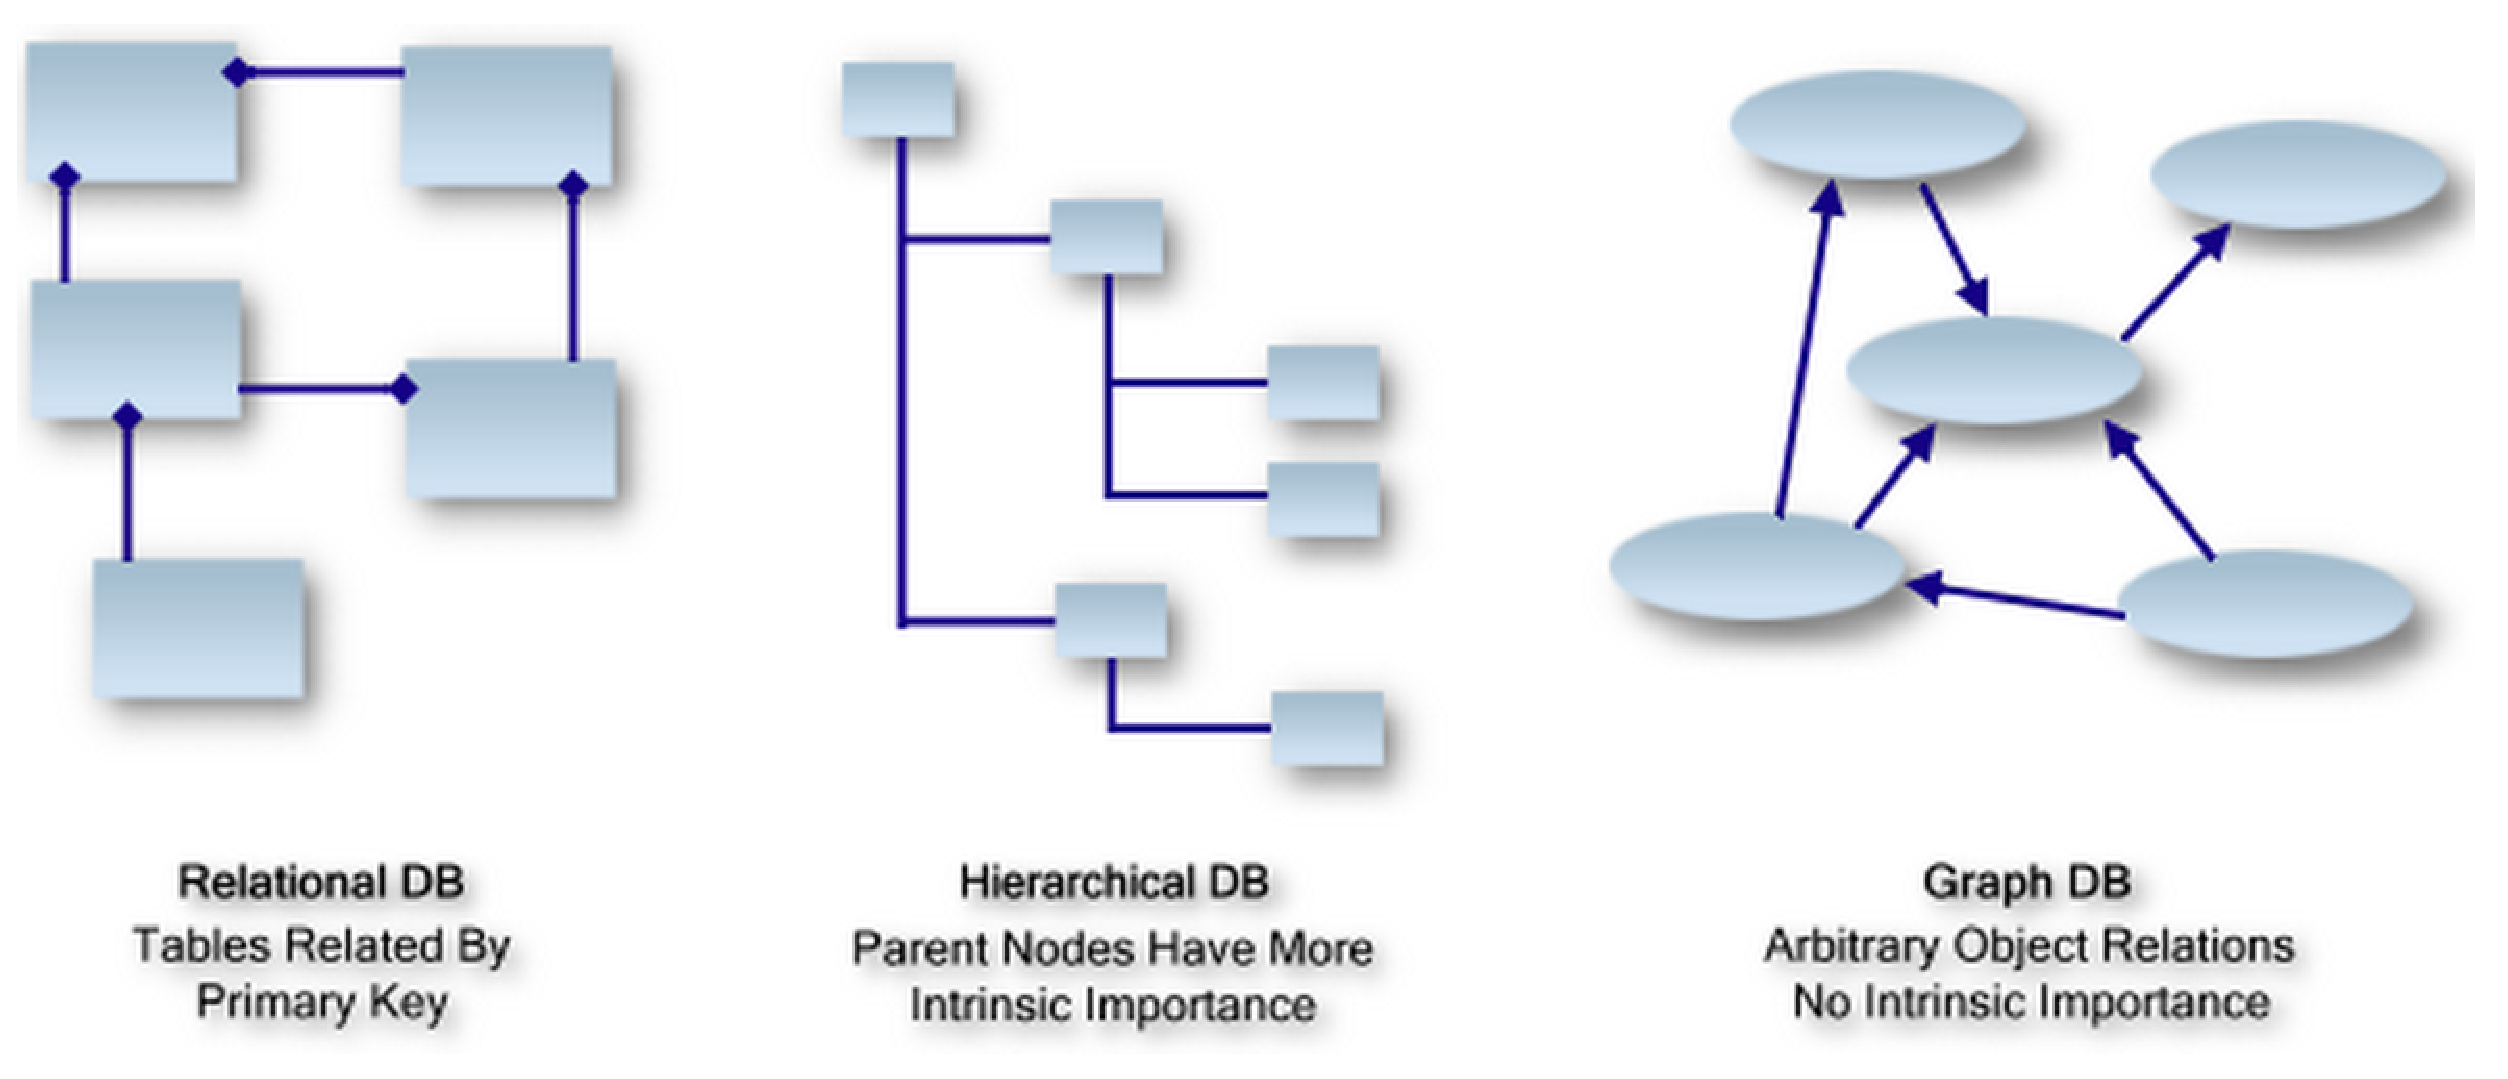
\includegraphics[height=7cm,
    angle=0]{./images/data_models.eps}}
  \caption{(A) Relational DB (tables related by primary keys), (B) Hierachical DB (parent nodes), (C) Graph DB (arbitrary object relations)}
  \label{fig:data_models} 
\end{figure}


\section{RDBMS vs. NoSQL vs. Graph vs. Cloud databases}
\label{sec:database_categories}

Relational Database Management System (RDBMS) organizes data into tables (each
row is a record, and each column represents a field; with metadata containing
the constraints expressing the relation between these tables) and uses SQL
language to query data (Chap.\ref{chap:SQL_lang}).
As the result, the structure of the database is described using well-structured
schemas. Read Sect.\ref{sec:RDBMS}

NoSQL-like databases do not use SQL-language, and suppor unstructured data, i.e.
the number of columns can be different at diffferent rows in one
table/docucment/object. In addition to table, other concept can be used, e.g.
documents, objects. A NoSQL database can be local, e.g. BerkeleyDB or
distributed, e.g. HBase, MongoDB. It can be classified into
\begin{itemize}
  \item object-oriented: Sect.\ref{sec:NoSQL_object-oriented}
  \item document-oriented: Sect.\ref{sec:NoSQL_document-oriented}
\end{itemize}

A {\bf graph database} is a database that uses graph structures for semantic
queries with nodes, edges and properties to represent and store data.
Every element contains a direct pointer to its adjacent elements and no index
lookups are necessary. Read Sect.\ref{sec:Graph_database}.


A cloud database is a database that typically runs on a cloud computing platform. 
This is not a new form of database, i.e. the database can be any of the above type. 
Read Sect.\ref{sec:Cloud_database}.

 


\section{RDBMS}
\label{sec:RDBMS}

RDBMS was first introduced in 1969 by Edgar F. Codd.
\begin{enumerate}
  \item it is a group of tables
  \item each table contains rows, columns and primary key
  \item relationship between tables are maintained using foreign key
  \item query language: SQL
\end{enumerate}

SQL was first introduced for Edgar F. Codd's relational model
(Chap.\ref{chap:SQL_lang}).

To guarantee database integrity when changing the data, {\bf database
transactions} are defined. Properties are ACID
\begin{itemize}
  \item Atomicity: the operations on database for a single transaction either
  all occur or nothing
  
  \item Consistency: ensure the integrity constraints during database operations
  \item Isolation: one operation is invisible to other concurrent operation
  \item Durability: ensure the transaction survive permanently
\end{itemize}


To optimize database structure, {\bf database normalization} is required
\begin{enumerate}
  \item organize tables and fields to minimize redundancy and dependency
  
  Devidie large tables into small tables with relations: 1NF, 2NF, 3NF, BCNF
  (Boyce-Codd Normal Form)
  
  \item a RDBMS is described as normalized if it is in 3NF (third normal form)
\end{enumerate}
Without normalization, it becomes difficult to handle and update database,
without facing data loss.

1NF = no two rows of data contains repeating group of information. So, each
table should have a unique value for each row, known as {\bf primary key}. The
primary key values are usually organized into a single column.

2NF = there is no partial dependency of any column on primary key. When a table
have more two or more columns as primary key (i.e. concatenated primary key),
then the value in each column that is not part of the primary key must depend
upon the entire concatenated key, not just part of it.

3NF = every non-prime attribute of the table must depend on the primary key. The
{\it transitive functional dependency} should be removed from the table.
Example:
\begin{verbatim}
Student_id   Student_name  DoB  Street city State Zip
\end{verbatim}
Here, street, city and state depend on zip. The dependency between Zip column
and other fields is called transitive dependency. Thus, a new table must be
created.

BCNF = a higher version of 3NF, in which a 3NF table that doesn't have multiple
overlapping candidate key is said to be in BCNF.

\begin{figure}[hbt]
  \centerline{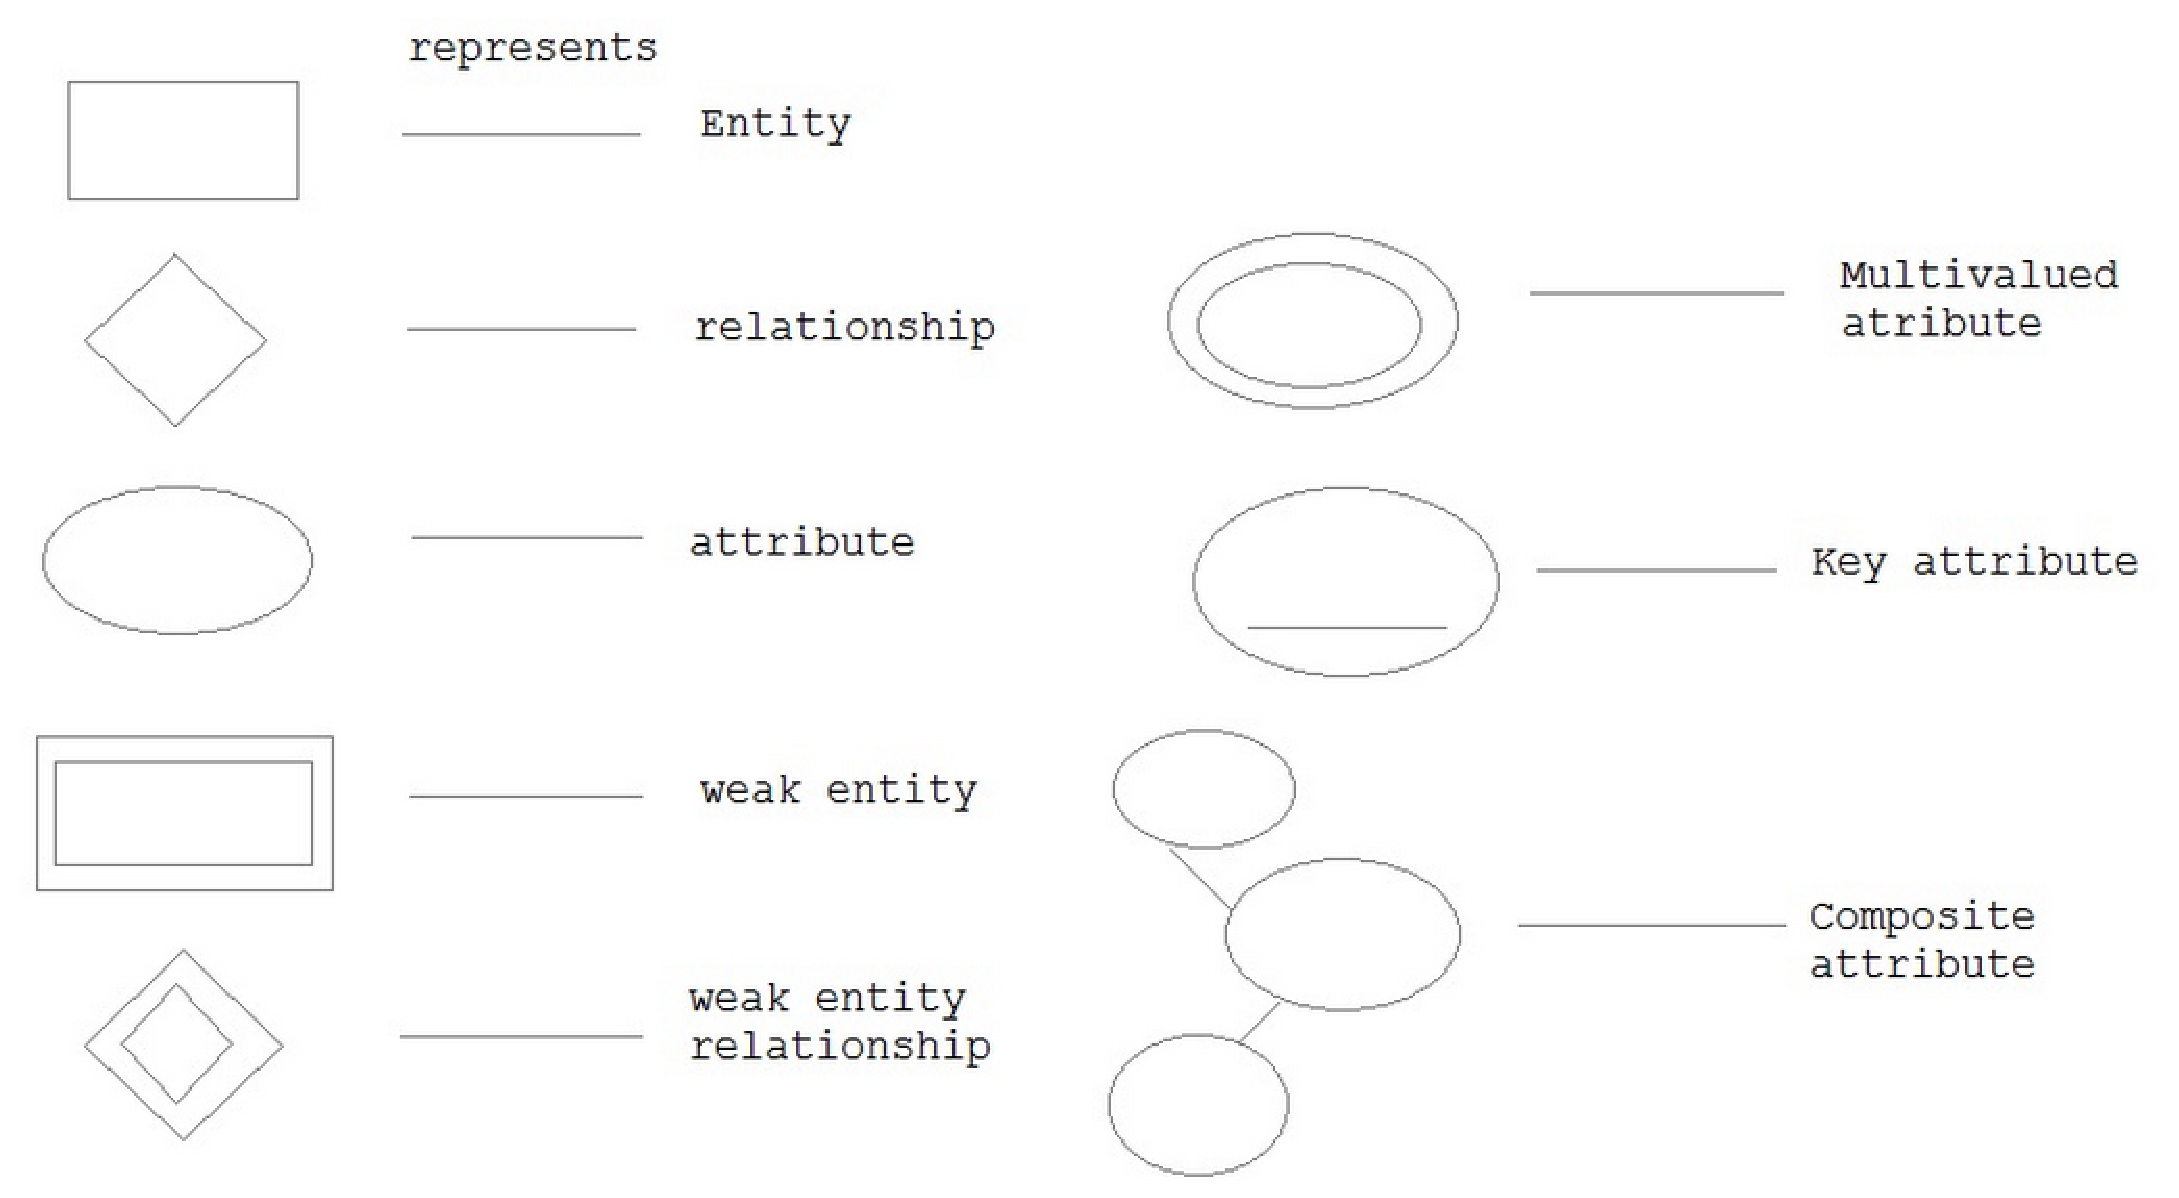
\includegraphics[height=6cm,
    angle=0]{./images/table-relationship.eps}}
\caption{Table relationship used in E-R diagram}
\label{fig:table-relationship}
\end{figure}

The relationship (dependency) between tables is represented using E-r diagram,
Fig.\ref{fig:table-relationship}.
\url{http://www.studytonight.com/dbms/er-diagram.php}

%\subsection{Softwares}

These software use SQL language to query/change data
\begin{enumerate}
  \item MySQL
  \item Microsoft SQL Server
  \item Oracle
  \item Infomix
  \item Sybase
  \item MS Access
  \item MariaDB
  \item PostgreSQL
\end{enumerate}

\subsection{Oracle}
The first commercial SQL based RDBMS is Oracle in 1977 when Lary Ellison first
saw a paper from IBM Journal of Research and Development that describes a
prototype for a RDBMS. He and coworkers Bob Miner and Ed Oates at Ampex formed
the Oracle company.
\begin{itemize}
  \item Oracle 1 (1978) written in assembly, never released
  \item Oracle 2 (1979)
  \item Oracle 3 (1983) written in C, first to run on mainframes, minicomputer
  and PCs
  \item Oracle 5 (1985) first to support client-server environment
  \item Oracle 6 (1988) allow multi-users to work on a single table, hot-backup,
  PL/SQL allow users to process data while it remains on databse
  
  \item Oracle 7 (1992) made major changes to structure and functions
  
  \item Oracle 7.3 (1996) support any type of data (text, video, map, sound,
  images)
  
  \item Oracle 9i (2001) improve performance, scalability and availability by
  allowing customers to use low-cost servers with Oracle Real Application
  Clusters
  
  \item Oracle 10g (2003) the first grid-computing product for enterprise, i.e.
  process the load based on demand
  
  \item Oracle 11g (2007) fast, reliable, secure and easys to manage all types
  of database workloads (enterprise applications, data warehouse, bid data
  analysis)
\end{itemize}
\url{http://www.slideshare.net/BcomBT/latest-trends-in-database-management}

\subsection{Microsoft SQL Server}

Microsoft SQL server
\begin{itemize}
  \item SQL Server 1.0 (1989): 16-bit
  \item SQL Server 1.1 (1991): 16-bit
  \item SQL Server 4.21 (1993): 
  \item SQL Server  6.0 (1995): 
  \item SQL Server 6.5 (1996)
  \item SQL Server 7.0 (1998)
  \item SQL Server 2000 (2000)
  \item SQL Server 2000 (2003): 64-bit
  \item SQL Server 2005 (2005): 
  \item SQL Server 2008 (2008)
  \item SQL Azure DB (2010): cloud-database
  \item SQL Server 2012 (2012): provide Mission Critical Confidence (greater
  uptime, fast performance and enhanced security features for mission critical
  workloads), Breakthrough Insight (managed self-service data exploration,
  stunning interactive data visualization capabilities)	
  \begin{itemize}
    \item data any types (structured or unstructured)
    \item any size (GB to PB)
    \item connecting with external data source (US Census Bureau, U.N.)
  \end{itemize}
\end{itemize}

\subsection{MySQL}

MySQL (most popular open-source RDBMS)
\begin{itemize}
  \item MySQL 1.0 (1994): originally developed by Michael Widenius and David
  Axmark
  \item MySQL 3.19 (1996)
  \item MySQL 3.21 (1997)
  \item MySQL 3.22 (1998)
  \item MySQL 3.23 (2000)
  \item MySQL 4.0 (2002)
  \item MySQL 4.01 (2003)
  \item MySQL 4.1 (2004)
  \item MySQL 5.0 (2005)
  \item 2008: acquired by Sun MicroSystems
  \item MySQL 5.1 (2008)
  \item 27-Jan-2010: Oracle acquired Sun MicroSystems
  \item MySQL 5.5 (2010)
  \item MySQL 5.6 (2011): enable next generation web-based and embedded
  applications and services
\end{itemize}

\subsection{MariaDB}

MariaDB (open source) created by some of the original authors of MySQL, lead by
Michael Widenius
\begin{itemize}
  \item MariaDB 5.1 (2009)
  \item \ldots
  \item MariaDB 10.0.0 (2012): 
  \begin{itemize}
    \item more storage engine than MySQL
    \item speed better than MySQL
    \item new features: GIS functionality, etc.
    \item truly open source
  \end{itemize}
\end{itemize}

\subsection{PostgreSQL}

PostgreSQL (most advanced open-source RDBMS): ACID-compliant
\begin{itemize}
  \item PostgreSQL 1.0 (1996)
  \item PostgreSQL 6.0 (1997)
  \item PostgreSQL 7.0 (2000)
  \item PostgreSQL 8.0 (2005)
  \item PostgreSQL 9.0 (2010)
  \begin{itemize}
    \item object-relational database system
    \item nested transactions
    \item international character sets
    \item spatial database for GIS
\end{itemize}
\end{itemize}

\subsection{Amazon Aurora}
\label{sec:Aurora}

\subsection{NuoDB}
\label{sec:NuoDB}


\section{Distributed Databases}

A distributed database is a database in which a storage devices are not all
attached to a common processing unit such as the CPU, i.e. 
collections of data (e.g. in a database) are distributed across multiple
physical locations (e.g. on the Internet, on the corporate intranets, etc.).

\section{NewSQL}
\label{sec:NewSQL_database}

This is a new idea proposed in 2011. As NoSQL solutions cannot give up strong
transactional and consistency requirement like SQL, to deal with large financial
and order processing systems the only options previously available for these
organizations were to either (1) purchase a more powerful single-node machine or
(2) develop custom middleware that distributes queries over traditional DBMS
nodes. Both are prohibitively expensive and only a few big companies can affort.

NewSQL combines the power of NoSQL and maintains ACID property of SQL.
There are two types
\begin{enumerate}
  \item  completely new database platforms (redesign from scratch): each node
  keeps a subset of the data, i.e. share nothing nodes. 
  
  Examples: 
   Google Spanner, Clustrix, VoltDB, MemSQL, Pivotal's SQLFire and GemFire XD,
  SAP HANA, FoundationDB, NuoDB, TransLattice, ActorDB, and Trafodion.
  
  \item optimize storage engine for SQL: 
  
  Example:  TokuDB and InfiniDB.
\end{enumerate}

\url{http://en.wikipedia.org/wiki/NewSQL}

\subsection{TokuDB}
\label{sec:TokuDB}

\subsection{InfiniDB}
\label{sec:InfiniDB}

\subsection{VoltDB}

\subsection{MemSQL}

\subsection{ActorDB}

\subsection{Google Spanner}

\subsection{Clustrix}

\subsection{Pivotal's SQLFire + GemFire XD}	

\subsection{SAP HANA}

\subsection{FoundationDB}

\subsection{NuoDB}

\subsection{TransLattice}

\subsection{Trafodion}


\section{Cloud database (CDBMS)}
\label{sec:Cloud_database}

A cloud database is the one that runs on a cloud computing platform (large
number of computers interconnected through a real-time communication network,
e.g. Internet) (Sect.\ref{chap:cloud_computing}). 
A cloud database can be either a SQL-based or no-SQL-based data model. In other
words, a traditional database or NoSQL can be extended to support cloud. The
major drawback is {\bf security} and {\bf privacy issues}. 


There are three methods to run a database on the cloud:
\begin{itemize}
  \item using virtual machine image: user purchase a machine instance, for a
  limited time, and run the database with optimized-installation on these
  machine. user can also have the option to upload their own machine image
  with a database installed onit.
  
  In any way, the user still need to control and manage their database.
  
  \item Database as-a-Service (DBaas): the user do not need to install or
  maintain the database. Instead, the database service provider takes
  responsibility for installing and maintaining the database, and the user pay
  according to their usage.
  
  \item The database, even though hosted on the cloud, but is not offered as a
  service. The user can ask the cloud provider to manage it on the user's
  behalf. SQL databases are difficult to scale, meaning they are not natively
  suited to a cloud environment, although there are attempts to address this
  challenge for SQL-based database service. NoSQL databases are more
  suitedfor the cloud as it can scale up/down easily.
  
  Example: service by Rackspace (manage hosting for MySQL or NoSQL on dedicated
  and cloud architectures), service by Object Rocket (manage hosting for
  MongoDB)
\end{itemize}

The following companies provide services belong to one of the three categories
above
\begin{enumerate}
  \item MongoLab
  \item Microsoft SQL Azure DB
  
  \item Rackspace Cloud Database
  \item Amazon RDS: 3 database services (SimpleDB, Amazon RDS,
  DynamoDB)
  
  \item Google Cloud SQL
  \item Oracle Cloud
  \end{enumerate}

\subsection{Rackspace Cloud}

It use MySQL database, built on OpenStack (open source software cloud computing
software platform - Sect.\ref{chap:OpenStack}).

\subsection{Amazon Cloud}

Amazon RDS (Relational Database Service) give us accesses to the familiar MySQL,
Oracle or Microsoft SQL Server database engine. This can be done via different
DB Instance class.


Each customer has an instance with pre-configured parameters, automated backup

\subsection{Google Cloud}

Google Cloud allows customers to create, configure and use a RDBMS that live in
the Cloud.
\begin{itemize}
  \item easy-to-use:
  \item exceptional security
\end{itemize}


\subsection{MongoLab}



\subsection{Microsoft SQL Azure DB}

SQL Azure DB (2010)



\section{NoSQL (document-oriented)}
\label{sec:NoSQL}
\label{sec:NoSQL_document-oriented}

NoSQL is useful when working with huge quantitaty of data (e.g. big data) when
the data nature does not require a relational model. NoSQL provides mechanism to
store and retrieve data that use looser consistency models than traditional
RDBMS. Example: Hadoop, MongoDB, CouchDB, Oracle NoSQL Database, OrientDB,
Apache Cassandra.

So, NoSQL doesn't focus on the relationship between elements; but the capability
to store and retreieve great quantitatives of data. 
\begin{itemize}
  \item elastic scaling: low-cost commodity hardware, scaling easy
  \item big data:
  \item economics: use clusters of cheap commodity servers to manage the
  exploding data and transaction volumes
  \item flexible data model: more relaxed or even nonexistent data model
  restrictions
\end{itemize}


Current challenges
\begin{itemize}
  \item relatively new compared to RDBMS: many key features have yet be
  implemented
  \item support: most NoSQL projects are open-source
  \item few features to support analytics and business intelligence: even simple
  queries requires significant programming expertises
  \item administration: current NoSQl requires strong skills to install and to
  maintain
  \item not many experts: almost every NoSQL developer is in learning mode
\end{itemize}

Key datatypes in NoSQL
\begin{verbatim}
Key-value pair
Wide column
Graph
Document
Object
XML
\end{verbatim}

Document-oriented No-SQL databases can use either of the following format as
the native format:
\begin{itemize}
  \item XML: BaseX (Sect.\ref{sec:BaseX}), eXistDB (Sect.\ref{sec:eXistDB}),
  MarkLogic (Sect.\ref{sec:MarkLogic}), Sedna (Sect.\ref{sec:Sedna})
  
 These databases use XML as an interface to specify documents as tree structured
 data that may contain unstructured text, but on disk the data is stored as
 {\bf "optimized binary files."} This makes query and retrieval faster.
MarkLogic also allows XML and JSON to co-exist in one binary format.  
  
  \item JSON: 
\end{itemize}

NOTE: Some RDBMS databases also support handle XML type query, e.g.
\begin{verbatim}
SELECT
   id, vol, xmlquery('$j/name', passing journal AS "j") AS name
FROM
   journals
WHERE 
   xmlexists('$j[licence="CreativeCommons"]', passing journal AS "j")
\end{verbatim}
though using the native format of XML or JSON is faster.

\subsection{MongoDB}
\label{sec:MongoDB}

MongoDB (open-source, currently the most popular NoSQL) developed by 10gen in
Oct, 2007.
\begin{itemize}
  \item store structured data as JSON-like documents with dynamic schemas
  (format: BSON): make the integration of data in certain types of application
  easier and faster. It doesn't use table, but collection concept (wrapped by
  \verb!{  }!)
  
  As you can see, it is document-oriented storage
  \begin{verbatim}
{
"_id" : ObjectID("...."),
"Last name": "Dumont",
"First name": "Jean",
"DoB": "01-11-2010"
},

{
...
}
  \end{verbatim}
  
  \item SQL support? No
  
  query language: a rich, ad-hoc query language of its own
  (don't use SQL language)
  
  \item used by: MTV Networks, FourSquares, UIDA
\end{itemize}

When to use
\begin{itemize}
  \item general-purpose design: content management system, mobile applications,
  gaming, e-commerce, analytics, archiving, and logging
  
  \item don't require ACID transactions; yet provide some basic transactional
  capabilities with atomic operations.
  
  \item write in MongDB can be 'D'urable.
\end{itemize}

When not to use
\begin{itemize}
  \item systems that require SQL, joins, and multi-oriented transactions
\end{itemize}

\subsection{CouchDB}
\label{sec:CouchDB}

Apache CouchDB (open source) first released in 2005, and become Apache project
in 2008
\begin{itemize}
  \item use JSON-like format: store data as a collection of independent
  documents
  
  \item Javascript as the query language: a database system that completely
  embrace the web
  
  \item ACID semantics
  
  \item Security and Validations
  
  \item Distributed Updates and Replications
\end{itemize}


\subsection{Riak}
\label{sec:Riak}



\subsection{Oracle NoSQL database}

Oracle NoSQL 
\begin{itemize}
  \item a distributed key-value database
  
 data is stored as key-value pairs
 
 \item No Single Point of Failure design: ensure the system continues to run and
 data remain available after any failure
\end{itemize}

\subsection{OrientDB}

OrientDB (open source) written in Java
\begin{itemize}
  \item use JSON-like format:
  
  \item GraphDB: native management of graphs 
   
  A document-based database system, but the relationships are managed as
  in graph databases with direct connections between records
  
  \item amazing fast: store 150,000 records per second on common hardware
  
  \item support advanced features: ACID transactions, fast indexes, native and
  SQL queries
  
  \item support SQL? Yes with extensions to handle relationship without SQL join
  
  \item Web-ready: natively support HTTP, RESTful protocol, JSON without 3rd
  party libraries and documents
  
  \item run everywhere: pure 100\% Java
\end{itemize}

\subsection{Apache Cassandra}

Apache Cassandra (open source), a top-level project of Apache
\begin{itemize}
  \item initially developed by Facebook to power their Inbox Search feature
  until late 2010
  
  released as an open source project on Google code (Jul-2008). became an Apache
  Incubator project in Mar-2009; and got to top-level project in Feb-2010.
  
  \item distributed database management system
  \item fault-tolerance: data is replicated to multiple nodes
  \item performant: outperform popular NoSQL alternatives
  \item decentralized: no single point of failures $\rightarrow$ durable
  (suitable for applications that can't afford loss of data)
  
  Every node in the cluster are identical $\rightarrow$ not suitable for very
  large database
\end{itemize}

\subsection{Amazon DynamoDB}
\label{sec:DynamoDB}


Amazon DynamoDB is a no-SQL database engine developed by Amazon to use on their
EC2 cloud compute platform. However, there is a version to be downloaded and use
on local system to test DynamoDB-backed applications locally.


DynamoDB exposes a similar data model and derives its name from Dynamo, but has
a different underlying implementation. Dynamo had a multi-master design
requiring the client to resolve version conflicts and DynamoDB use synchronous
replication across multiple datacenters for high durability and
availability.

\subsection{ArangoDB}
\label{sec:ArangoDB}


\subsection{BaseX}
\label{sec:BaseX}

\subsection{eXistDB}
\label{sec:eXistDB}

\subsection{MarkLogic}
\label{sec:MarkLogic}

\subsection{Sedna}
\label{sec:Sedna}

Sedna is a free native XML database which provides a full range of core database
services - persistent storage, ACID transactions, security, indices, hot backup.
Flexible XML processing facilities include W3C XQuery implementation, tight
integration of XQuery with full-text search facilities and a node-level update
language.

Sedna is designed with the goal of providing a balance in performance between
XML queries and updates execution.
\url{http://www.sedna.org/}

\section{NoSQL (object-oriented)}
\label{sec:NoSQL_object-oriented}

\subsection{NeoDatis}

NeoDatis ODB which is an object-oriented database (not a document-oriented like
CouchDB or MongoDB). It has a very low memory footprint and supports database file encrytption.

\url{http://stackoverflow.com/questions/2516752/anyone-using-nosql-databases-for-medical-record-storage}

\section{Graph Database}
\label{sec:Graph_database}

The graph database is the data storage model used by semantic Web
(Chap.\ref{chap:GraphData_LargeScale}).


\section{Search engine}
\label{sec:search_engines}

Popular search engines are given in
\url{http://db-engines.com/en/ranking/search+engine}

\begin{enumerate}
  \item Solr (Sect.\ref{sec:Solr})
  \item ElasticSearch
  \item Splunk
  \item Sphinx
  \item Endeca
  \item MarkLogic
  \item Google Search
\end{enumerate}
Chap.\ref{chap:Desktop_SearchEngine} and Chap.\ref{chap:Web_SearchEngines}

\section{NoSQL (multi-model)}

A NoSQL multi-model database provide both document-oriented, object-oriented,
graph-oriented, key-value, Schema-less
\begin{itemize}
  \item OrientDB
  \item ArangoDB

\url{http://vschart.com/compare/arangodb/vs/orientdb}


\end{itemize}



\section{MapReduce}
\label{sec:MapReduce}

MapReduce is a distributed programming model introduced by Google which
typically requires a distributed filesystem, and an associated database system 
\begin{enumerate}
  \item Google MapReduce: use Google Bigtable database
  (Chap.\ref{chap:google_bigtable}) on Google Distributed Filesystem (GDFS)
  \item Apache Hadoop (Sect.\ref{chap:Hadoop}): use Hadoop file system (HDFS)
  with HBase database
  
  HBase features data compression, in-memory operation and Bloom filter.
  However, it is not as performant as HDFS in a MapReduce context, and can be 4
  to 5 times slower.

  \item Couchdb (Sect.\ref{sec:CouchDB})
  \item Infinispan
  \item MongoDB (Sect.\ref{sec:MongoDB})
  \item Riak
\end{enumerate}

Unlike MPI, MapReduce is designed for cloud-based distributed system, that can
deals with fault tolerance, and the large datasets are splitted into smaller,
more manageable size, which are then processed by multiple {\bf map} instances.
The results produced by individual {\bf map} instances are then set to the {\bf
reducers}, which collate their partial results to produce the final. 
The system scale well with the number of processors, i.e. less job for each map
instance, and thus speed up the process. This
map-reduce process can occur at multiple iteration. 

MapReduce tasks must be written as acyclic dataflow programs, i.e. a stateless
mapper followed by a stateless reducer, that are executed by a batch job
scheduler. This paradigm makes repeated querying of datasets difficult and
imposes limitations that are felt in fields such as machine learning, where
iterative algorithms that revisit a single working set multiple times are the
norm. To overcome this problem, several packages have been developed targetting
machine learning: Apache Spark, Apache Mahout, etc.

Applications that can benefit from this Map-Reduce programming paradigm:
machine learning, information retrieval, graph theory, visualization, \ldots

The original Map-Reduce use file-based communication. The variants can use
stream-based communication, e.g. NaradaBrokering streaming substrate (e.g. a set
of coorperating router nodes known as broker or proxy nodes).

\section{Locking model for a Database}


\begin{itemize}
  \item MVCC (multi-version concurrency control)
  
  \url{http://vschart.com/list/multiversion-concurrency-control/}
  
  \item Optimistic Locking
  
  \url{http://vschart.com/list/optimistic-locking/}
  
  \item Lock on write
  
  \url{http://vschart.com/list/lock-on-write/}
\end{itemize}
\import*{../Website_Builder/}{REST.tex}
\chapter{SQL Language}
\label{chap:SQL_lang}


SQL was first introduced for Edgar F. Codd's relational model. It has 2 parts
\begin{enumerate}
  \item data definition language (DDL)
  
  Commands: CREATE, ALTER (add/modify/remove/rename columns to existing table
  with ADD, MODIFY, DROP, RENAME), TRUNCATE (remove all data but not delete the
  table structure), RENAME (table)
  
  \item data manipulation laguage (DML)
  
  Commands: CRUD (Create, Read, Update, Delete) can be done via INSERT, MERGE,
  UPDATE, DELETE
\end{enumerate}
Newer parts
\begin{enumerate}
  \item Transaction contrl language (TCL)
  
  commands: COMMIT, ROLLBACK, SAVEPOINT
  
  \item Data control language (DCL): grant or take back control authority
  
  commands: GRANT, REVOKE
  
  \item Data query language (DQL)
  
  commands: SELECT
\end{enumerate}

\import*{../Website_Builder/}{RDF.tex}
\chapter{Storage Model for XML data}


The Extensible Markup Language (XML) is an
emerging standard for data representation and
exchange on the Internet.

\section{XML query language}

Several XML query languages were proposed including
Lorel [Abiteboul et al., 1997], XML QL
[Deutsch et al., 1999a], XML-GL [Ceri et al., 1999],
Quilt [Chamberlin et al., 2000], YATL
[Cluet et al., 1998], XPath [Clark and DeRose, 1999]
and XQuery [Chamberlin et al., 2001].
The surveys on XML schema languages
and query languages can be found in
[Bonifati and Ceri, 2000, Lee and Chu, 2000a].

\section{Persistent XML data storage model}

An XML document can be represented as a graph, Fig.\ref{fig:XML_graph}, or an
{\bf XML data graph}. Because elements of an XML document are ordered, in an XML
data graph, the
\begin{itemize}
  \item {\it ordinal} of an element is the order of this element among all siblings that
share the same parent

At level 2: the ordinal of node \verb!&2! is 1, and node \verb!&4! is 3.

  \item {\it label-path} in an XML data graph is a dot-separated sequence of
  edge-labels
  
A label-path such as \verb!DBGroup.Member.Office.Room!.  
  
  \item {\it data-path} is a dot-separated alternating sequence of element
  nodes.
  
A data-path such as \verb!&1.&3.&11.&18!
\end{itemize}
Suppose we have a data-path $e_0.e_1.e_2. ... .e_n$ with $e_o$ is the virtual
root ($e_o$ is obmitted when we refer to the data-path), and a label-path
$l_1.l_2.l_3. ... .l_n$ for that data-path.

\begin{figure}[hbt]
  \centerline{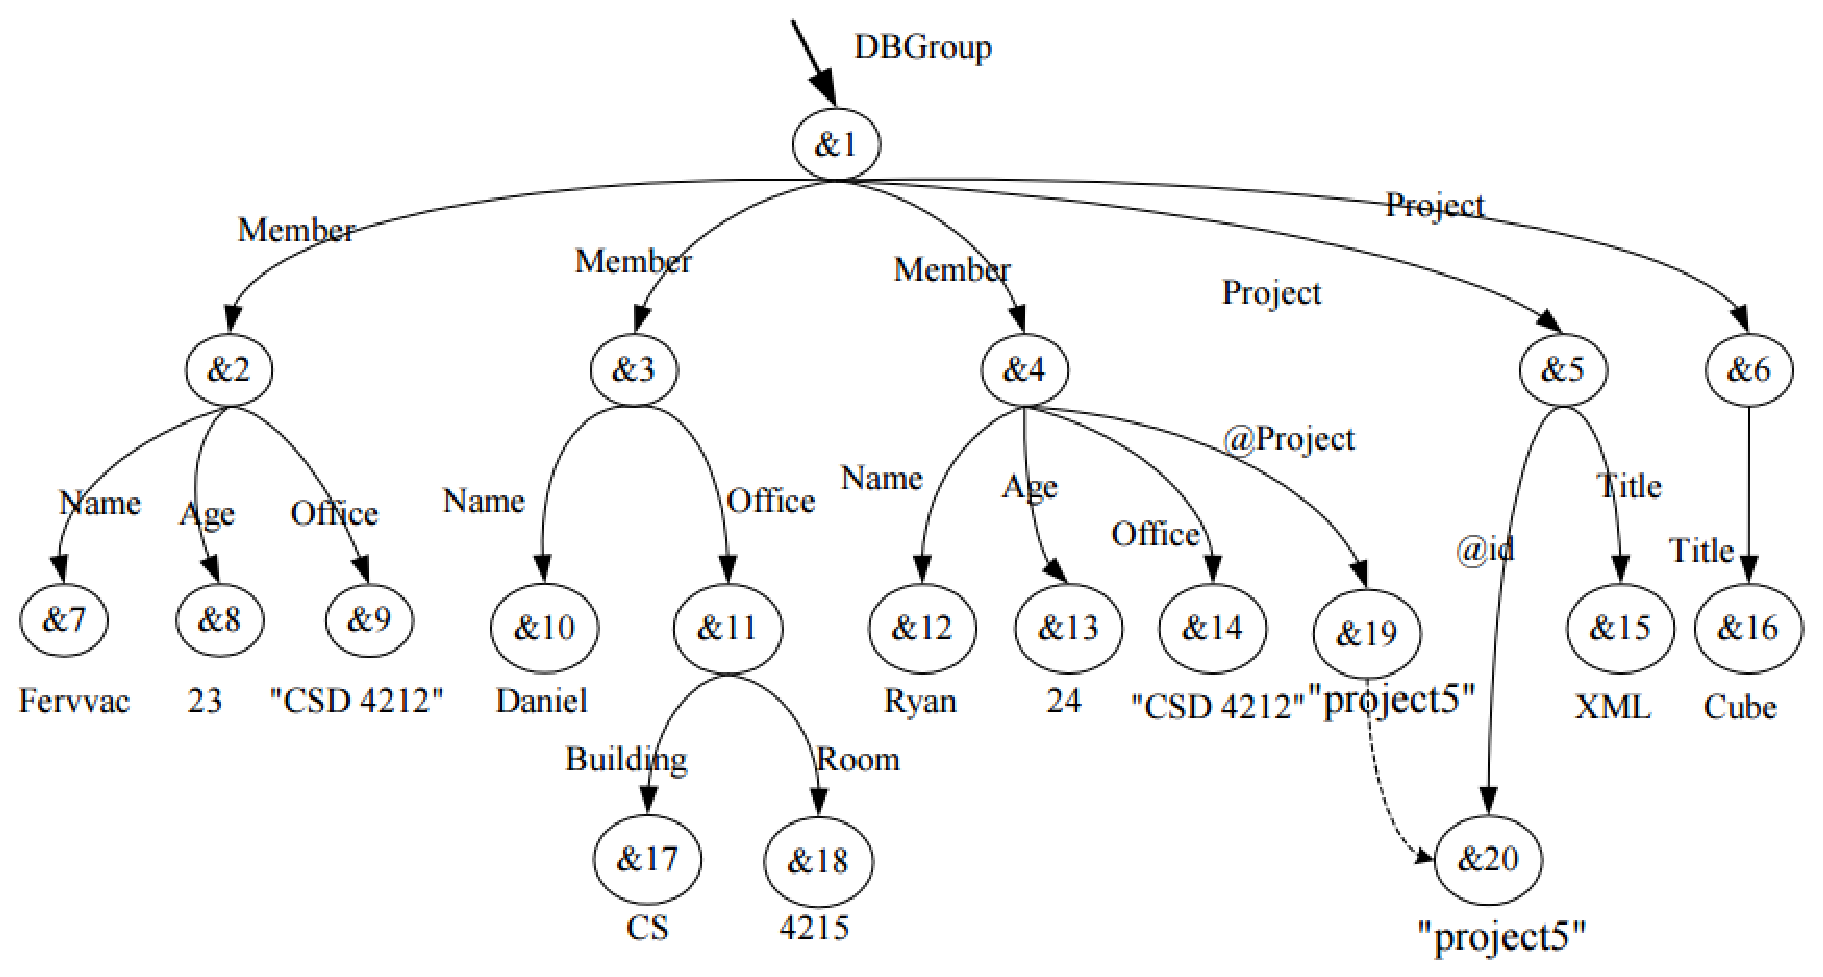
\includegraphics[height=5cm,
    angle=0]{./images/XML_graph.eps}}
\caption{A data graph for a small XML document}
\label{fig:XML_graph}
\end{figure}


The problem of storage model design for storing
XML data becomes a database schema design
problem, which can be classified into 2 categories:
\begin{itemize}
  \item {\bf structure-mapping approach} 
  
Here, the design of database schema is based on the understanding of DTD
(Document Type Descriptor) that describes the structure of XML documents.
  
  \item {\bf model-mapping approach}: 
  \begin{itemize}
    \item edge-oriented: Edge, Monet, XParent (Sect.\ref{sec:XParent}).
    
    Monet is different from the other twos; as Monet did not use a fixed schema.
    
    \item node-oriented: XRel
  
  There is no edge information explicitly maintained in this schema.
  \end{itemize}
  
Here, a fixed database schema is used to store any XML documents without
assistance of DTD,
\end{itemize}



\subsection{Edge}
\label{sec:Edge}

Edge approach uses a single table name Edge
\begin{verbatim}
Edge(Source, Ordinal, Target, Label, Flag, Value)
\end{verbatim}
to store both the label edge and data edge 
\begin{equation*}
(l_i, e_{i-1},e_i)
\end{equation*}


\subsection{Monet}
\label{sec:Monet}

Monet is a variant of Edge approach (Sect.\ref{sec:Edge}).
With Monet, all the tables are smaller. But the number of tables is huge,
because it needs to create a table for each distinctive label-path.

\subsection{XRel}
\label{sec:XRel}

XRel stores XML data graphs in four tables. They are Path, Element, Text, and
Attribute.
\begin{verbatim}
Path(PathID, Pathexp)
Element(DocId, PathID, Start, End, Ordinal)
Text(DocId, PathID, Start, End, Value)
Attribute(DocId, PathID, Start, End, Value)
\end{verbatim}
The unique feature of XRel is that no node identifiers
are needed to store XML data graphs. Instead, start
and end positions are used, which is denoted as a {\bf region}.


\subsection{XParent}
\label{sec:XParent}

It adopts the data model of XPath (Sect.\ref{sec:XPath}) to represent
XML documents.
XPath data model models XML documents as an
ordered tree using 7 types of nodes, namely, root,
element, text, attribute, namespace, processinginstruction
and comment.

XParent uses four types: root, element, text and attribute.
XParent is a four table database schema, LabelPath, DataPath, Element and Data
as follows
\begin{verbatim}
LabelPath(ID, Len, Path)
DataPath(Pid, Cid)
Element(PathID, Did, Ordinal)
Data(PathID, Did, Ordinal, Value)

\end{verbatim}

It is (a) a four table schema; b) it explicitly maintains both labelpaths
(sequences of element tags) and data-paths (sequences of elements) in two separate but
interrelated tables. The label-paths give a global view on the XML documents
stored in the database management system. As for the data-paths, two formats are
considered. The first keeps parent-child relationships.
The second further materializes it by maintaining ancestor-descendant
relationships. We call them path materialization.


 

\part{Cloud Computing}
\import*{../Sys_admin/}{VirtualMachine.tex}
\chapter{Virtualization - Hypervisor (Virtual Machine Monitor - VMM)}
\label{chap:Hypervisor}

%\section{Virtualization - Hypervisor (Virtual Machine Monitor - VMM)}

Hypervisor is the agent that helps you create virtual machines.
Hypervisor is the guy who creates and runs the guest machine and provide the
host’s resource to the guest. 

\section{Review}

\subsection{User-mode Linux (UML)}

UML allows a Linux kernel to run as a user process (like any other Linux
process, such as Emacs or Vim) within a "host" Linux operating system.

This interesting technology has a number of advantages, such as the ability to
run any recent UML-enabled kernel of choice (including one different from the
kernel of the host system) and the ability to debug the kernel of the guest
system more easily.



\subsection{Full virtualization}

When many people think of virtualization, they think about full virtualization
software that emulates a virtual machine all the way down to the hardware level
and lets an operating system run on top of that emulated hardware. This is the
approach taken by several well-known software packages such as VMware, QEMU, and
Bochs.

Example of hypervisors
\begin{enumerate}
  \item QEMU 
  
  \item KVM 
  
  KVM helps QEMU to access hardware virtualization features on different
  architectures.
  It also adds the acceleration feature to the QEMU process. So, in short, when
  they are together, QEMU is the hypervisor/emulator and KVM is the accelerating
  agent.
  
\end{enumerate}

Full virtualization software does extensive virtualization of hardware,
including the processor, BIOS, and I/O devices. One of the advantages of this
approach is that just about any operating system can be run on the virtual
hardware. One disadvantage is that emulating down to the hardware layer involves
a lot of overhead, which usually results in a noticeable performance degradation
for the guest and host operating system.

\subsection{paravirtualization}

Virtualization technologies such as KVM and Xen, which started by booting
separate virtual systems on emulated hardware and then attempted to lower their
overhead via paravirtualization and related mechanisms.


Recent years have seen a lot of interest in another virtualization technique
called paravirtualization. With paravirtualization, virtual machines run inside
a virtual machine monitor (VMM), or hypervisor, and access its services through
a software interface.

Paravirtualization is actually an old technique dating back to IBM mainframes,
but lately it's increasingly being applied to personal computers with software
such as Parallels Workstation and Xen.


Paravirtualization does have drawbacks, though, as it typically requires either
the guest operating system to be modified to support the hypervisor, or specific
hardware support in newer Intel and AMD processors.


\section{Virtualization \& Hypervisors}

You are running on Windows platform, but you want to test software running on
Linux platform on the same machine, without rebooting the PC; then it comes
{\bf virtualization} and the tools are called {\bf hypervisor}.

\subsection{Virtualization}


{\bf Virtualization} refers to the creation of a virtual (rather than actual)
version of something, e.g. an O/S or a machine or a storage device or a network
resource.
\begin{itemize}
  \item \textcolor{red}{O/S virtualization} (or virtual machine): the most
  prevalent form of virtualization

  \item \textcolor{red}{Application Virtualization} (aka thin clients): you run
  a program locally, but all the binaries, running states, \ldots are stored on,
  managed, and delivered by a remote machine. Your local machine provide the CPU
  and RAM required to run the application, but nothing is installed locally on
  your own machine.
  
  
  \item \textcolor{red}{Application Server Virtualization} (often used in
  advanced load balancing): one server is presented to the outer-world, hiding the
  availability of multiple servers. This public server runs as a reverse 
  proxy load balancer (an appliance or servie that provide access to many
  different application services transparently) and provides a virtual interface
  (Virtual IP or VIP), represent itself as the actual web server.
  
% multiple web servers or applications are managed by a load balancer
   \item \textcolor{red}{Management virtualization} : (1) virtual IP management
   and segmentation, e.g. VLAN (a single Ethernet port may support multiple
   virtual connections from multiple IP addresses and networks, but they are
   virtually segmented using VLAN tags, e.g. eth0:1 virtual network adapters).
   (2) virtual routing tables (typically a routing table and an IP network share
   a 1:1 relationship, even though a single port may host multiple virtual
   interfaces).
   
   Each virtual IP connection over this single physical port is independent and
   unaware of other's existence, but the switch is aware of each unique
   connection and manage each one independently.
   
   
   
   
   \item \textcolor{red}{Network virtualization}: 
   
 %  \item 
\end{itemize}
\url{https://www.f5.com/pdf/white-papers/virtualization-defined-wp.pdf}

\subsection{Hypervisor}
\label{sec:hypervisor}


A {\bf hypervisor} is a class of software  which is tasked with creating,
releasing, and managing the resources of "guest" operating systems, or virtual
machines. Hypervisor is used on VPS (Sect.\ref{sec:VPS}). Examples of
hypervisors are VMware (Sect.\ref{sec:VMWare_ESXi}), HyperV
(Sect.\ref{sec:Hyper-V}).

{\bf Hypervisor} is a system comprised of computer software, firmware + hardware
that creates a virtual machine that enable deploying any guest operating system
easily, Fig.\ref{fig:Hypervisor}. 

\section{Type-1 and Type-2 hypervisors}
\label{sec:hypervisor-type-I}
\label{sec:hypervisor-type-II}


There are two types of hypervisor (Sect.\ref{sec:hypervisor}): Type-1 and Type-2.


As Type-1 is faster, Type 1 hypervisors provide {\it server} (i.e. no GUI)
virtualization on bare metal hardware, whereas Type 2 hypervisors typically
provide {\it desktop} virtualization based on an existing operating system.



\begin{itemize}
  
  \item {\bf Type-1} (bare-metal hypervisor): the hypervisor runs directly on
  the host's hardware to control the hardware and manage the guest O/S. For this
  reason, they are aka {\bf bare metal hypervisors}. The guest O/S runs as a
  process on the host.
  
\begin{verbatim}
your apps
----------------
Guest O/S
----------------
Type-I hypervisor
----------------
hardware
\end{verbatim}
  

  Example: Oracle VM Server for SPARC, Oracle VM Server for x86, Microsoft
  Hyper-V 2008/2012 (Sect.\ref{sec:Hyper-V}).
  
  Xen hypervisor project is the only open-source Type-1 hypervisor (Sect.\ref{sec:Xen}).
  
  \item {\bf Type-2} (hosted hypervisor): these hypervisors run like a
  conventional computer programs, and provides the environment to host a guest
  O/S.  

\begin{verbatim}
your apps
----------------
Guest O/S  [e.g. Linux]
----------------
Type-2 hypervisor  (provide software emulation, mapping from Linux-based to Windows-based)
----------------
host O/S [e.g. Windows]
----------------
hardware
\end{verbatim}

Early virtualization efforts relied on software emulation to replace hardware
functionality. But software emulation can be a slow and inefficient process.
Because many virtualization tasks were handled through software, VM behavior and
resource control were often poor, resulting in unacceptable VM performance on
the server. Sect.\ref{sec:virtualization_hardware} discusses how ntel Corp. and
AMD addressed this problem by creating processor extensions that could offload
the repetitive and inefficient work from the software.


  
  Example: VirtualBox, VMWare Workstations programs.
\end{itemize}

The computer on which hypervisor is running is called the {\bf host machine}.
The hardware/firmware/software - collective form a virtual machine - on which
the guest O/S running is not necessary the same as the
hardware/firmware/software of the host machine, as the hyeprvisor can emulate
that. Each virtual machine is called a {\bf guest machine}. Multiple instances
of a variety of O/S may share the virtualized hardware resources.
\url{http://www.ibm.com/developerworks/cloud/library/cl-hypervisorcompare/}
 
\begin{figure}[hbt]
  \centerline{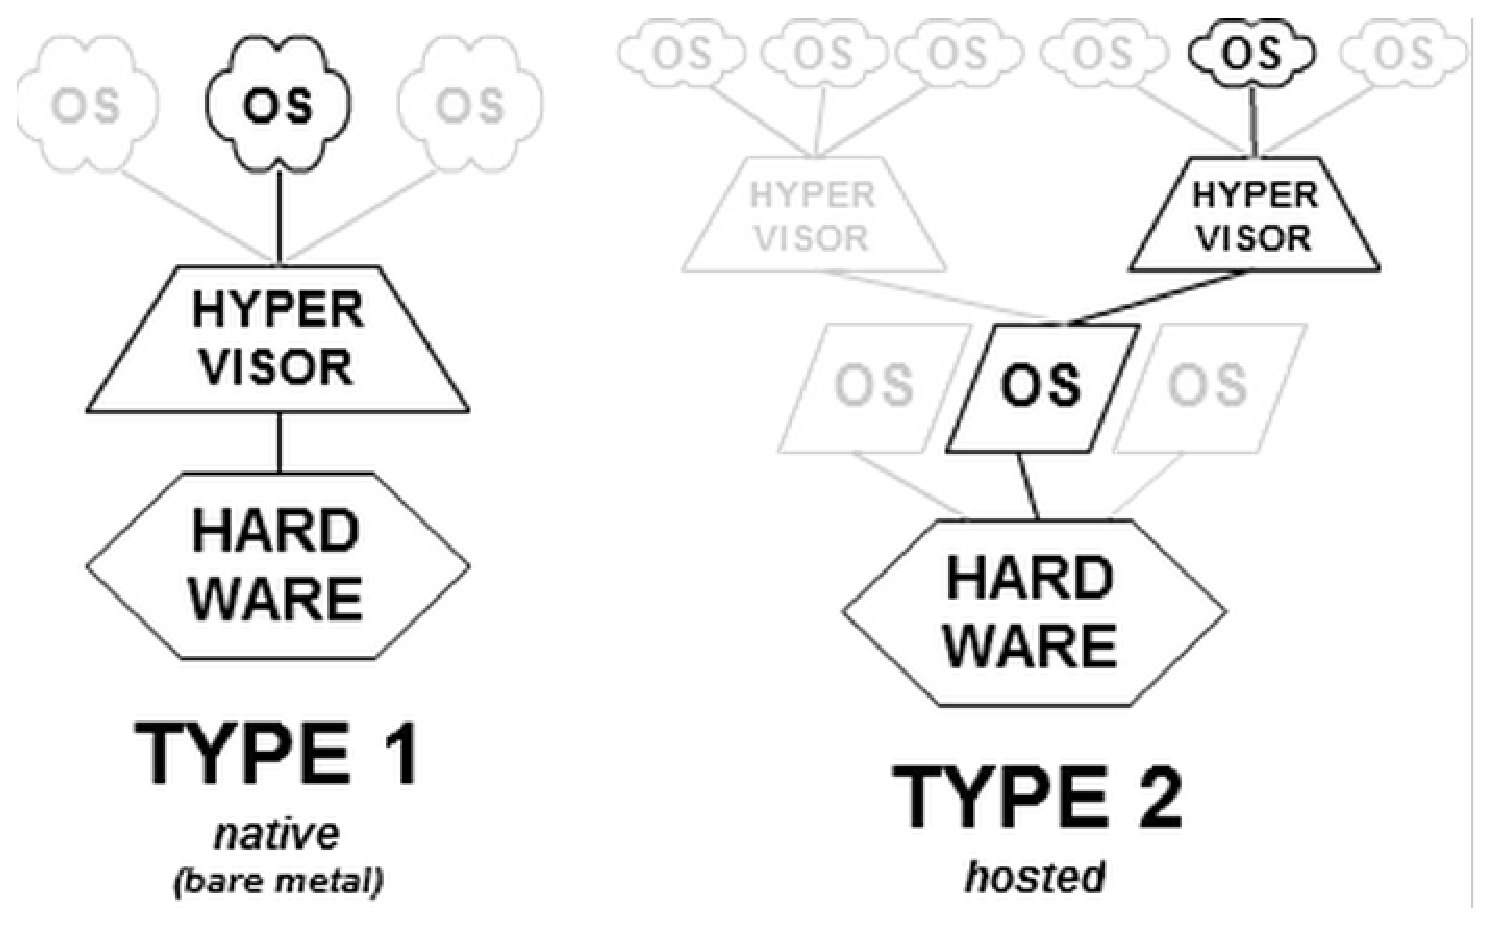
\includegraphics[height=6cm,
    angle=0]{./images/Hypervisor.eps}}
\caption{Type-1 and Type-2 hypervisors}
\label{fig:Hypervisor}
\end{figure}

All hypervisors are not made equal, but they all offer similar features.
Understanding the features they have as well as the guest operating systems each
supports is an essential aspect of any hardware virtualization hypervisor
selection process.

 Review:
\url{http://www.flexiant.com/2014/02/12/hypervisor-comparison-kvm-xen-vmware-hyper-v/}

\section{Hardware support for virtualization}
\label{sec:virtualization_hardware}


Early virtualization efforts relied on software emulation to replace hardware
functionality which is slow. Both Intel Corp. and AMD addressed this problem by
creating processor extensions that could offload the repetitive and inefficient
work from the software. By handling these tasks through processor extensions,
traps and emulation of virtualization, tasks through the operating system were
essentially eliminated, vastly improving VM performance on the physical server.


To enable sharing hardware easily, extra hardware components were granually
added to manage that, e.g. since 2006 Intel (VT-x, codename Vanderpool) and
since 2004 for AMD (AMD-V, codename Pacifica) to allow simpler virtualization
software. Later on, many other technologies have been developed.

\begin{itemize}
  
  \item {\bf first generation}: AMD-V and Intel VT-x
  
  \item {\bf second generation}: AMD-V/RVI (Rapid Virtualization Indexing, or
  former name Nested Page Tables) which is adopted by Intel under a different name:
  Extended Page Tables (VT-x/EPT).
  
NOTE: A study by VMware found that RVI offers up to 42\% gains in performance
compared with software-only (shadow page table), and one by RedHat found 200\%
in performance for OLTP benchmark.
   
\end{itemize}

To check on Ubuntu
\begin{verbatim}
egrep -c '(vmx|svm)' /proc/cpuinfo
\end{verbatim}
\verb!0! = no hardware virtualization. If 1, it supports, but make sure it is
enabled in the BIOS. 

\subsection{AMD-V and Intel VT-x}
\label{sec:AMD-V}

\begin{enumerate}
  \item in 2004: AMD-V (AMD virtualization) is a set of hardware extensions for the X86 processor architecture.

added to AMD's Pacifica 64-bit x86 processor designs
  
in 2006: 2006, AMD's Athlon 64 X2 and Athlon 64 FX processors appeared with
AMD-V technology, and today, the technology is available on Turion 64 X2,
second- and third-generation Opteron, Phenom and Phenom II processors.
  
\end{enumerate}




Open BIOS, you can enable the feature:	Intel Virtualization Technology (also
known as Intel VT) or AMD-V on your CPU chip. 

When enabled and the CPU chip supports, an input/output memory management unit
(IOMMU) allows guest virtual machines to directly use peripheral devices, such
as Ethernet, accelerated graphics cards, and hard-drive controllers, through DMA
and interrupt remapping. This makes the guest O/S runs much faster, than
tradititional virtual machines.


\subsection{AMD-V/RVI and Intel VT-x/EPT}
\label{sec:AMD-V/RVI}

\url{https://support.amd.com/en-us/kb-articles/Pages/GPU120AMDRVICPUsHyperVWin8.aspx}

AMD processors that support AMD Virtualization (AMD-V) Technology with Rapid
Virtualization Indexing (RVI), also known as nested page tables or Second Level
Address Translation (SLAT) necessary to support Hyper-V virtualization
technology in Microsoft Windows 8.



\section{KVM (type-1)}
\label{sec:KVM}

{\bf KVM} (Kernel-based Virtual Machine) is the Linux-based Open-source
Hypervisor, first introduced in 2007. KVM supports native virtualization on
processors with hardware virtualization extensions (e.g. x86 processors, ARM,
IA-64, x86-64, PowerPC, S/390), and guest operating systems including many
variations of Linux, BSD, Solaris, Windows, Haiku, ReactOS, and the AROS
Research Operating System (there's even a modified version of qemu that can use
KVM to run Mac OS X).

It is being used in Redhat Enterprise Virtualization (RHEV).
\url{http://www.linux-kvm.org/page/Main_Page}

To run KVM, you need a processor that supports hardware virtualization
(Sect.\ref{sec:virtualization_hardware}). To setup KVM in Ubuntu
\url{https://help.ubuntu.com/community/KVM/Installation}

\section{Xen (Type-1)}
\label{sec:Xen}
\label{sec:Xen-hypervisor}


An open source hypervisor which originated in a 2003 Cambridge University
research project. Its \verb!dom0! host runs on Linux, which in turns run on Xen.
It was originally supported by XenSource Inc, which was acquired by Citrix Inc in 2007.

\ref{sec:hypervisor-type-I}

\section{VMWare's ESXi (type-1, for server)}
\label{sec:VMWare_ESXi}

VMware ESX's enterprise software hypervisors (VMWare vSphere) run directly on
server hardware without requiring an additional underlying operating system.
VMware's hypervisor is very mature and extremely stable.

The obsolete version (since 2011) is VMWare Server.

\section{VMWare Player (for desktop)}
\label{sec:VMWare_Player}

VMWare Player:
\url{https://my.vmware.com/web/vmware/free#desktop_end_user_computing/vmware_player/4_0}

If you run Linux as the guest O/S, it may ask you to install
Linux tool.

To enable shared-folder, we use
\url{https://www.vmware.com/support/ws5/doc/ws_running_shared_folders.html}

VMWare Player
\begin{itemize}
  \item 6.0: support new O/S (Windows 8.1), VM (16 vCPUs, 8TB, virtual SATA controller, USB3)
\end{itemize}

\section{Hyper-V}
\label{sec:Hyper-V}

Hyper-V is a commercial hypervisor provided by Microsoft, running on Windows but
can host any O/S supported by the hardware platform. 


\section{App-V (app virtualization)}
\label{sec:App-V}

Microsoft Application Virtualization (App-V, Softricity SoftGrid) is an 
application virtualization and application streaming solution from Microsoft.

App-V technology allows applications to be deployed ("streamed") in real-time to
any client from a virtual application server, i.e. no need to install locally
(although a standalone deployment is still supported).

The App-V client needs to be installed on the client machines and application
data that is stored on the virtual application server is installed (streamed) to
the client cache on demand when it is first used, or pre-installed in a local
cache.

Different versions of the same application can be run under App-V concurrently
and so that mutually exclusive applications can co-exist on the same system.

\url{https://en.wikipedia.org/wiki/Microsoft_App-V}

\section{z/VM (IBM, type-1)}

z/VM runs on IBM's zSeries and can be used to support large numbers (thousands)
of Linux virtual machines.

\section{PowerVM (type-2)}

PowerVM is a feature of IBM POWER5, POWER6, and POWER7 servers, support
provided for it on IBM i, AIX, and Linux O/S.

\section{VirtualBox (type-2)}
\label{sec:VirtualBox}

 VirtualBox works on multiple platforms with easy installation and setup.  It
 can run on Windows, Linux, Macintosh, and Solaris hosts, and supports host
 installation of Windows (NT 4.0, 2000, XP, Server 2003, Vista, Windows 7,
 Windows 8), DOS/Windows 3.x, Linux (2.4, 2.6 and 3.x), Solaris and OpenSolaris,
 OS/2, and OpenBSD.
 
Among the compelling features, VirtualBox makes running multiple OS guests easy;
your limits are primarly dictated by your system memory and CPU capability.

\chapter{Isolation (O/S-level virtualization) - Container}

\section{History of container runtime}
\label{sec:container-technology-history}

Since system administration is a difficult task, many tools have been developed
to make life easier for the administrator. These tools often enhance the way
systems are installed, configured, and maintained. One of the tools which can be
used to enhance the security of a FreeBSD system is jails (Sect.\ref{sec:jail}).

This {\bf Operating-system-level virtualization},
also known as containerization, refers to an operating system feature in which
the kernel allows the existence of multiple isolated user-space instances.

So, a {\bf container} is like a virtual environment, in that a software can
run in isolation of other software running on the physical host machine.
There is no spec specifying what a container should implement.
There are several Linux-based Containers projects:

The container technology is not new, but is getting so popular recently
primarily because kernel support is now available in Linux (namespace and
cgroups) kernel 3.8 (Feb 2013).

There have been different implementations of a container runtime to support
launching a container

\begin{enumerate}
  
  \item chroot - Sect.\ref{sec:chroot}
  
  \item Jails (FreeBSD) - Sect.\ref{sec:jail}
  \item Zones (Solaris) - Sect.\ref{sec:zones-Solaris}
  
  \item Google container: use cgroup of the kernel (Sect.\ref{sec:cgroups})
  
  \url{https://github.com/google/lmctfy}

  \item OpenVZ (depends on custom kernel) - Sect.\ref{sec:OpenVZ}
  \item WPARs (AIX O/S - Workload PARtitions)
  
  \item Linux VServer (depends on custom kernel)
  
  \url{http://linux-vserver.org/}
  
  
  \item OpenVZ: based on modified kernel - Sect.\ref{sec:OpenVZ}
  
  
  \item Linux-based container (LXC): Sect.\ref{sec:LXC} from 2014
  
  \item Docker - Sect.\ref{sec:Docker} - the company and the technology it provides that really makes
  container-like technology becomes popular.
\end{enumerate}

Review: \url{http://ramirose.wix.com/ramirosen} 


\subsection{Linux namespace}

In namespaces, you start with no isolation, from zero, and you add whatever you
want — mount, PID, network, hostname, user, IPC namespaces.


In Linux namespaces,  user isolation is done with weird UID mapping ("uid
1 in the container is uid 1000001 outside") and PID isolation I don't even know
how, jails are at their core just one more column in the process table. PID,
UID, and now JID (Jail ID). (The host is JID 0.) No need for weird mappings, the
system just takes JID into account when answering system calls.



Jails are actually very similar to Linux namespaces / unshare. But unlike Linux
namespace (which starts with nothing), in jails, you start with a reasonable
secure baseline — processes, users, POSIX IPC and mounts are always isolated.
But! You can isolate the filesystem root — or not (by specifying /). You can
keep the host networking or restrict IP addresses or create a virtual interface.
You can isolate SysV IPC (yay postgres!) — or keep the host IPC namespace, or
ban IPC outright. See? The interesting parts are still flexible! Okay, not as
flexible as "sharing PIDs with one jail and IPC with another", but still.

\url{https://news.ycombinator.com/item?id=13982620}


\subsection{1979: Unix V7 with chroot}
\label{sec:chroot}

During the unix history of containers development of Unix V7 in 1979, the chroot
system call was introduced, changing the root directory of a process and its
children to a new location in the filesystem. This advance was the beginning
process isolation: segregating file access for each process.


\verb!chroot! utility is used to change the {\it root directory} (which is '/'
by default) of a running process and all of its children, to some subtree of the larger file system.

Example: change the root to /mnt/arch and we have defined the shell.
\begin{verbatim}
chroot /mnt/arch /usr/bin/bash
\end{verbatim}

\verb!chroot! modifies pathname lookups for a process and its children so that
any reference to a path starting '/' will effectively have the new root, which
is passed as the single argument, prepended onto the path.


This technique is commonly used to improve computer security by placing a
vulnerable server process in a chroot jail that is isolated from the rest of the
system.

NOTE: Calls to chroot() do not stack, with additional calls essentially
overwriting the existing one.


A process/command that runs in such a modified environment cannot access files
outside the given root directory. If we change from '/' to \verb!/chroot/named! as
root directory, then within this chroot jail, /etc/passwd, for example, would
map to /chroot/named/etc/passwd in the main file system.

SYNTAX:
\begin{verbatim}

chroot /path/to/new/root /path/to/server

chroot [options] /path/to/new/root /path/to/server

	–userspec=USER:GROUP : This option describe the user and group which is to be used.
	
	–groups=G_LIST : It describe the supplementary groups as g1,g2,..,gN.
\end{verbatim}

Example:
\begin{verbatim}
# create a “jail” directory inside the “home” directory, which will be our new root.

mkdir $HOME/jail


mkdir -p $HOME/jail/{bin, lib64}
cd $HOME/jail

# copy essential files, 
# /bin/bash and /bin/ls into $HOME/jail/bin/ location

cp -v /bin/{bash, ls} $HOME/jail/bin


# find what other essential libraries
ldd /bin/bash

# ... and copies these libraries
cp -v libraries/displayed/by/above/command $HOME/jail/lib64

# finally, issue 'chroot'

sudo chroot $HOME/jail /bin/bash
\end{verbatim}


%Suppose you're running a process, from the directory 'A', now, from within the
%process, you want the process to receive directory 'B' as the base-folder, then
%you issue 'chroot' command within the process.

Processes created in the chrooted environment can not access files or resources
outside of it.  In a traditional chroot environment, processes are only limited
in the part of the file system they can access. The rest of the system
resources, system users, running processes, and the networking subsystem are
shared by the chrooted processes and the processes of the host system.


\begin{mdframed}


The use of the term "chroot jail" in the manpage is unfortunate as it may help
perpetuate a common misconception about chroot(). It often gets mentioned in the
same context as the "jail" calls for the BSDs, but it has little in common with
them.

\url{https://lwn.net/Articles/252794/}

Chroot was added to BSD in 1982. 
\url{https://www.freebsd.org/cgi/man.cgi?query=chroot&sektion=2&manpath=freebsd-release-ports}
\end{mdframed}

\subsection{2000: jail utility - FreeBSD Jail}
\label{sec:jail}

jail have been available since FreeBSD 4.X, and is buit upon the \verb!chroot!
concept (Sect.\ref{sec:chroot}) which has long been supported by many UNIX
kernels, including the Linux kernel.

COMMAND SYNTAX:
\url{https://www.freebsd.org/cgi/man.cgi?query=jail&sektion=8&manpath=freebsd-release-ports}

\verb!jail! helps to create a containerized environment for a running process
and its children like \verb!chroot!; but with more complexity.
A BSD jail is a mini-virtualization that partitions a system into multiple
virtual systems each of which can have its own root account. chroot() has none
of that sophistication.

\verb!chroot! is suited to easy tasks which do not require much flexibility or
complex, advanced features. With chroot, it only isolate the file systems, while
the rest of the system resources, system users, running processes, and the
networking subsystem are shared by the chrooted processes and the processes of
the host system.

Jails expand this model by virtualizing access to the file system, the set of
users, and the networking subsystem. More fine-grained controls are available
for tuning the access of a jailed environment. Jails can be considered as a type
of operating system-level virtualization.

In each containerized environment or virtual system, jail provides it with an
own set of users and their own root account which are limited to the jail
environment. The root account of a jail is not allowed to perform operations to
the system outside of the associated jail environment.
\url{https://linux.die.net/man/8/jailkit}

IN SUMMARY: A jail is characterized by 4 elements
\begin{enumerate}
  \item a new root directory (like chroot provides)
  
  A directory subtree: the starting point from which a jail is entered. Once
  inside the jail, a process is not permitted to escape outside of this subtree.
  
  \item a hostname: which will be used by the jail.
  
  \item an IP address: which is assigned to the jail. The IP address of a jail
  is often an alias address for an existing network interface.

  \item a  command: the path name of an executable to run inside the jail. The
  path is relative to the root directory of the jail environment.
  
\end{enumerate}

Also, jails have their own set of users and their own root account which are
limited to the jail environment. The root account of a jail is not allowed to
perform operations to the system outside of the associated jail environment.

\url{https://www.freebsd.org/doc/handbook/jails.html}

% Jailkit is a set of utilities that can limit user accounts to a specific
% directory tree and to specific commands
% \begin{itemize}
%    \item Jailkit is a set of utilities to limit user accounts to specific files using chroot() and or specific commands.
%  
%   \item  A jail is a directory tree that you create within your file system; the
%   user cannot see any directories or files that are outside the jail directory
% \end{itemize}
% \urk{https://olivier.sessink.nl/jailkit/index.html#intro}

Example: 
\verb!jk_cp! can be used to copy a file or device into a jail.
\begin{verbatim}

mkdir /home/sftproot
chown root:root /home/sftproot

chmod 0755 /home/sftproot

# quickly create a jail with several files or directories needed for a specific
# task or profile.

jk_init -j /home/sftproot jk_lsh
jk_init -j /home/sftproot sftp
jk_init -j /home/sftproot scp

# Create the account
jk_addjailuser -j /home/sftproot test

# Edit the jk_lsh configfile in the jail; see man jk_lsh.

# You can use every editor you want; I choose 'joe'
joe /home/sftproot/etc/jailkit/jk_lsh.ini

# Restart jk_socketd so that log messages are transferred
killall jk_socketd
jk_socketd

# Test the account
sftp test@localhost
# Check the logs to see if everything is correct
tail /var/log/daemon.log /var/log/auth.log

\end{verbatim}



The jail utility creates new jails, or modifies or	removes	existing
jails.   \url{https://www.freebsd.org/doc/handbook/jails.html}

A jail (or	``prison'') is specified via parameters	on the command
line, or in the jail.conf file.
     

FreeBSD Jails allows administrators to partition a FreeBSD computer system into
several independent, smaller systems – called “jails” – with the ability to
assign an IP address for each system and configuration.

This achieve clear-cut separation between its services and those of its
customers for security and ease of administration.

\subsection{2001: util-vserver utility - Linux VServer (similar to FreeBSD Jail)}

Linux-VServer allows you to create lightweight virtual machines with little
overhead and great performance, while still providing increased security and
fault isolation. You can use it to create a secure and fault-tolerant system
without investing in additional hardware.
 
\verb!jail! was developed for Free BSD O/S. In GNU/Linux systems, an equivalent
system called Linux-VServer was developed to provide virtualization for
GNU/Linux systems, i.e. a simple way to run several virtual servers on one piece
of physical hardware.

Linux VServer allows to run multiple virtual units at once. Those units are
sufficiently isolated to guarantee the required security, but utilize available
resources efficiently, as they run on the same kernel.
\url{http://www.linux-vserver.org/Welcome_to_Linux-VServer.org}

Linux-VServer is composed of two parts: Code in the kernel (i.e. require
patching the Linux kernel) to support security contexts, and userspace tools for
creating and managing virtual servers. Experimental patches are still available,
but the last stable patch was released in 2006. Linux-VServer, and similar
software like OpenVZ, take a "lightweight" approach to virtualization,
essentially segmenting a single Linux kernel environment into virtual machines
with separate file systems, process tables, and network addresses.

As a result, the virtual machines, often called security contexts or Virtual
Private Servers (VPS) in Linux-VServer parlance, can run at nearly the full
speed of the underlying physical hardware.
Unlike some other virtualization approaches, all the virtual servers run under
the control of the same kernel. This minor limitation is often outweighed by the
increase in performance that you can achieve by running a single kernel

Also keep in mind that although you're limited to a single kernel for all your
virtual machines, there is no problem with running different Linux distributions
in your virtual machines (as long as those Linux distributions can work with the
chosen kernel).


A Linux kernel on the host O/S needs to have support for VServer security
contexts. You can either download a kernel built with this support, or you can
download a VServer patch that you can apply to your kernel source code before
building.
\url{https://www.linux.com/news/installing-linux-vserver}
 
 
\subsection{2004: zones -  Solaris Zones (formerly Solaris Containers)}
\label{sec:zones-Solaris}

Solaris Containers (including Solaris Zones) is an implementation of operating
system-level virtualization technology for x86 and SPARC systems, first released in 2005.

Oracle Solaris Zones technology is an Oracle Solaris feature that first showed
up in Solaris Express and Oracle Solaris 10 3/05 and was called Oracle Solaris
Containers. With Oracle Solaris 11, we now officially call the technology Oracle
Solaris Zones.


Oracle Solaris Zones and Linux Containers are virtualization technologies at the
application level, so they are "above" the OS kernel. With Oracle Solaris Zones
and Linux Containers, there is one OS kernel that is shared by many zones or
containers.

\url{https://www.oracle.com/technical-resources/articles/it-infrastructure/admin-zones-containers-virtualization.html}

Solaris Zones are more designed and an evolution from FreeBSD Jails.
We could say a zone is a "sandbox" that provides a playground for an
application.
\begin{enumerate}
  
  \item The global zone holds the Oracle Solaris kernel, the device drivers and
  devices, the memory management system, the file system and, in many cases, the
  network stack.
  
  The global zone sees all physical resources and provides common access to
  these resources to the non-global zones.
  Looking from the global zone, a non-global zone is just a bunch of processes
  grouped together by a tag called a zone ID.
  
  
  \item The other zones are called non-global zones and are isolated from each
  other, but they all share one global zone. Non-global zones have their own
  file systems, process namespace, security boundaries, and network addresses.
  
  The non-global zones appear to applications like separate Oracle Solaris
  installations.
  
   Based on requirements, non-global zones can also have their own network stack
   with separate network properties. And, yes, there also is a separate
   administrative login (root) for every non-global zone, but even as a
   privileged user, there is no way to break into one non-global zone from a
   neighboring non-global zone. 
  
\end{enumerate}

Solaris Zones are included in the Solaris 11 Common Criteria Evaluation for the
virtualisation extension (VIRT) to the OSPP. Solaris Zones are also the
foundation of our multi-level Trusted Extensions feature and is used for
separation of classified data by many government/military deployments around the
world. \url{https://blogs.oracle.com/solaris/overview-of-solaris-zones-security-models-v2}


The first public beta of Solaris Containers was released that combines system
resource controls and boundary separation provided by zones, which were able to
leverage features like snapshots and cloning from ZFS.

%\subsection{Solaris Zones (2005+)}

A zone is a virtualized operating system environment created within a single
instance of the Solaris OS. Within a zone, the operating system is represented
to the applications as virtual operating system environments that are isolated
and secure. The applications run in different zones with complete isolation,
while the underlying operating system resources are centrally managed and
administered.


%\subsection{2005: Open VZ}
\subsection{2005: OpenVZ (partial type-2: container hypervisor)}
\label{sec:OpenVZ}

OpenVZ (Open Virtuzzo) is an operating system-level virtualization technology
for Linux which uses a patched Linux kernel for virtualization, isolation,
resource management and checkpointing. The code was not released as part of the
official Linux kernel.


It is possible to run production containers today, but not with
the mainline kernel. Instead, one can use the modified kernel provided by the
open source OpenVZ project.  
\url{http://lwn.net/Articles/524952/}


The \verb!libvirt! library makes it possible to start up an application in a
container.

It has a modified Linux kernel (meaning host systems can only be some flavor of
GNU/Linux) that is tailored to support OpenVZ containers.

The system containers are containers which offer an environment as close to
possible as the one you'd get from a VM but without the overhead that comes with
running a separate kernel and simulating all the hardware (see
Sect.\ref{sec:linuxcontainers.org}).

\subsection{2006: cgroups - Linux feature (formerly Process Containers)}
%\label{sec:cgroups}

Check the Sect.\ref{sec:cgroups} in Sys-admin book.


\subsection{2008 (released 2013): liblxc library - Linux Containers - LXC (partial type-2)}
\label{sec:LXC}

Based on the new features of Linux kernels,  the Linux Containers project
started around 2006 to provide light-weight virtualization to the Linux kernel
as an external set of patches to the Linux kernel. It was first implemented in
2008 using
\begin{enumerate}
  \item cgroups - Sect.\ref{sec:cgroups}
  
   Linux kernel's control groups ("Cgroups") subsystem is used by LXC 
   to provide resource management
    
  
  \item Linux namespaces (Sect.\ref{sec:namespaces}),
  
  LXC provides resource isolation through process namespaces. 
  
\end{enumerate}
It works on a single Linux kernel without requiring any patches.

Linux Containers offer essentially native performance, and you can efficiently
manage resource allocation in real time.

\textcolor{red}{IMPORTANT}: Unlike full virtualization solutions and similar to
Oracle Solaris Zones, LXC will not let you run any other non-Linux operating
systems (such as proprietary operating systems or other types of UNIX). However,
you are able to run different Linux distributions on the same host kernel in
different containers. For example, you could run an instance of Oracle Linux 5
inside a container hosted on an Oracle Linux 6 system running the Unbreakable
Enterprise Kernel release 2.
\url{https://www.oracle.com/technical-resources/articles/it-infrastructure/admin-zones-containers-virtualization.html}

Unprivileged containers are containers that are run without any privilege. This
requires support for user namespaces in the kernel that the container is run on.
LXC was the first runtime to support unprivileged containers after user
namespaces were merged into the mainline kernel.
\begin{verbatim}
apt-get install lxc libvirt0 libpam-cgroup libpam-cgfs bridge-utils

\end{verbatim}

LXC was delivered in \verb!liblxc! library and provided language bindings for
the API in Python3, Python2, Lua, Go, Ruby, and Haskell. \verb!liblxc! library -
LXC (LinuX Containers) was the first, most complete implementation of a runtime
environment for a Linux container manager.
LXC is used as the default runtime for LXD, a container hypervisor exposing a
well-designed and stable REST-api on top of it (Sect.\ref{sec:LXD}).


Like OpenVZ (Sect.\ref{sec:OpenVZ}), LXC is a container technology.
LinuX Containers (LXC) is an operating system-level virtualization method for
running multiple isolated Linux systems (containers) on a single control host
(LXC host).

LXC's main focus is system containers. That is, containers which offer an
environment as close as possible as the one you'd get from a VM but without the
overhead that comes with running a separate kernel and simulating all the
hardware. This is achieved through a combination of kernel security features
such as namespaces, mandatory access control and control groups.



There is no need for a separate kernel under LXC since it takes root
in the host kernel. Like OpenVZ, LXC uses the resource management and
checkpointing of the host kernel. 

\begin{itemize}
 
  \item LXC 3.0: 
  
  \item LXC 2.0
   
  \item LXC 1.0 was released in February (20.2.2014).
  
  
LXC is included in Ubuntu 14.04.

  \item  LXC-0.9.0 was released, in April 2013.
  
 \end{itemize}

LXC helps to build a light-weight Linux virtual machines (i.e. an O/S container)
that you can launch this virtual machine on any computing machine; while Dockers
helps to build a container for an application (application container) so that it
contains required packages (with the minimal O/S components) so that the
application can run the same everywhere (Sect.\ref{sec:Docker}).

The LXC Project is supported by Ubuntu and powers Ubuntu Juju
(Sect.\ref{sec:Juju}). LXC is actively developed but not well documented beyond
Ubuntu. \url{http://www.flockport.com/lxc-vs-docker/}

The LXC project provides base OS container templates and a comprehensive set of tools for
container lifecycle management. It is currently led by a 2 member team, Stephane
Graber and Serge Hallyn from Ubuntu.   

LXC consists of a variety of container templates, standard tools for managing
containers, bindings for multiple languages (Ruby, Python, Go, Lua, etc), and
the \verb!liblxc! library (\verb!libvirt! is considered an alternative library).
LXC is free software, most of the code is released under the terms of the GNU
LGPL license

Docker (Sect.\ref{sec:Docker}) as developped by Docker, Inc is a container
system based on LXC container technology, has exploded in popularity.
\url{http://www.zdnet.com/article/ubuntu-is-working-on-a-new-secure-container-hypervisor-lxd/}

\subsection{-- install in Debian-based O/S}


\subsection{-- networking}

NOTE: most container templates configure the first interface to use DHCP by default.

\textcolor{red}{LXC 2.0+}:
Stretch ships with a new major release of LXC which also includes a helper for
easier networking setup called lxc-net lxc-net allows you to set up a simple
bridge for your containers, providing a DHCP-and-NATed IPv4 network. IPv6
support currently (in Stretch) requires manual configuration.

\url{https://wiki.debian.org/LXC}
 
\textcolor{red}{LXC 1.0+}:
 
Debian's packages do not ship any default network setup for containers
(/etc/lxc/default.conf contains lxc.network.type = empty).
If you want to have network in your containers (and you usually do), you will
have to either change the global default or configure each individual container.
You will also probably will have to setup a bridge, firewall and maybe DHCP (see
below for details how to do this).




\subsection{-- LinuxContainers.org: LXC, LXD, LXCFS, CGManager}
\label{sec:linuxcontainers.org}

Linuxcontainers.org is the umbrella project behind LXC, LXD, LXCFS and
CGManager.
\url{https://linuxcontainers.org/}

Glauber then looked at some examples of the various resource-isolation features
("namespaces") that have been added to the kernel.  Namespace and cgroups are
the LXC building blocks.
\begin{itemize}
  \item  A network namespace provides a private view of the network for a group
  of processes. 
  
  Network namespaces also make packet filtering easier, since each group of
  processes has its own network device.

  \item User namespaces provide isolation of the "user ID" resource.
  
  Thus, it is possible to create users that are visible only within a container.
    Most notably, user namespaces allow a container to have a user that has root
    privileges for operations inside the container without being privileged on
    the system as a whole.   
  \item Control groups (cgroups) provide the other piece of infrastructure
  needed to implement containers.
  
  A cgroup is a logical grouping of processes that can be used for resource
  management in the kernel. Once a cgroup has been created, processes can be
  migrated in and out of the cgroup via a pseudo-filesystem API.
  
  The CPU controller mechanism allows a system manager to control the percentage
     of CPU time given to a cgroup. The CPU controller can be used both to
     guarantee that a cgroup gets a guaranteed minimum percentage of CPU on the
     system, regardless of other load on the system, and also to set an upper
     limit on the amount of CPU time used by a cgroup, so that a rogue process
     can't consume all of the available CPU time.
\end{itemize}
\url{http://lwn.net/Articles/524952/}


\subsection{-- LXD (partial type-2)}
\label{sec:LXD}


LXD is building on top of a container technology called LXC which was used by
Docker before. However LXD allows you to have access to a virtual server, just
like you would have in case of a hypervisor. The big difference is that LXD does
not require operating systems to be duplicated.

Ubuntu develops a new secure container hypervisor: LXD (pronounced: lex-dee).
Containers are more efficient than virtual machines, but are potentially less
secure, as it accesses directly the host O/S.

\begin{figure}[hbt]
  \centerline{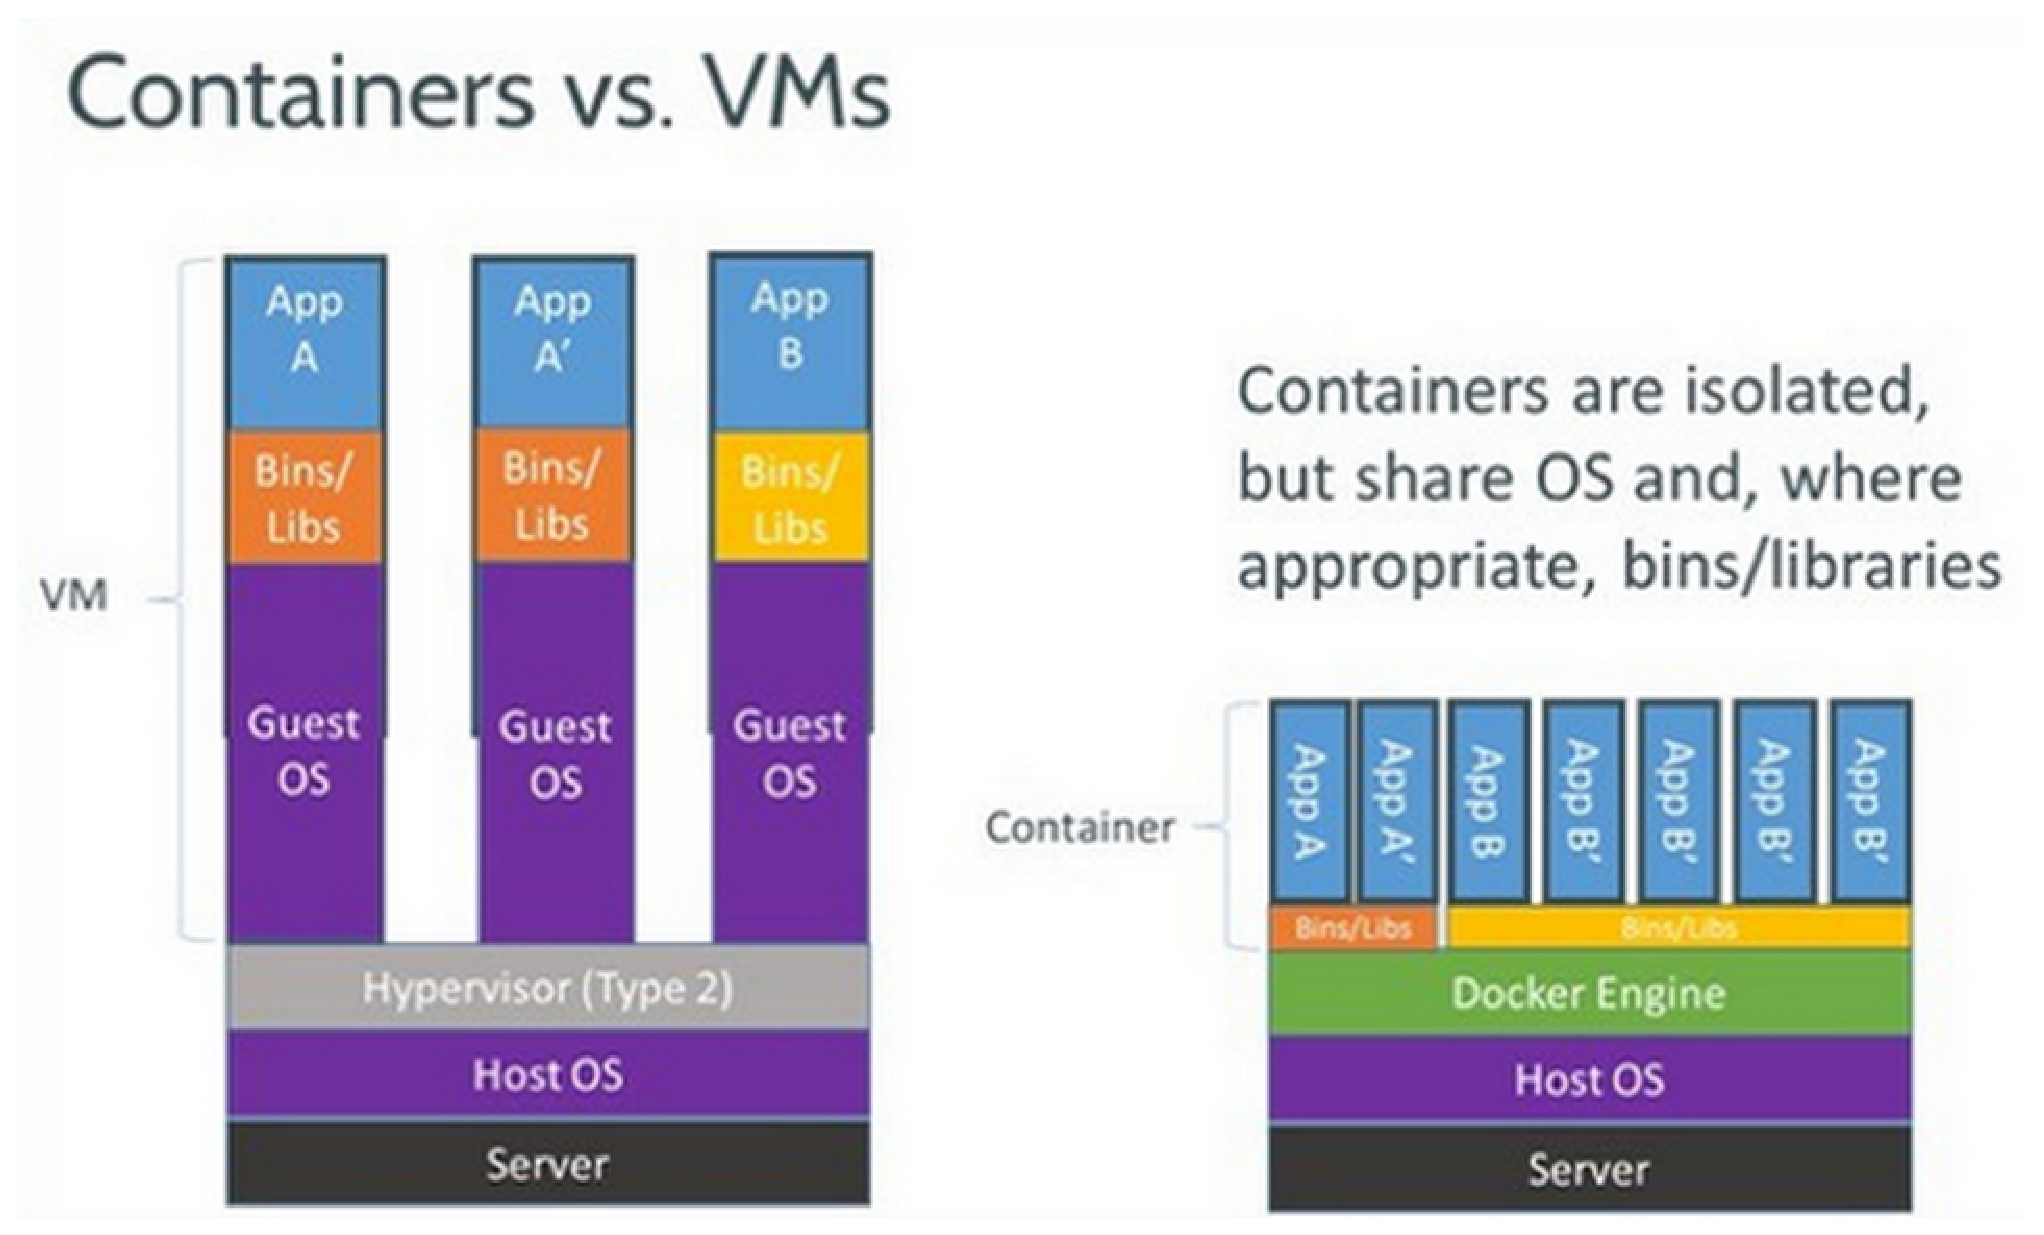
\includegraphics[height=8cm,
    angle=0]{./images/hypervisor_container.eps}}
\caption{Type-2 hypervisor with guest O/S (virtual machines) and Container}
\label{fig:hypervisor_container}
\end{figure}
 
Docker specializes in deploying apps (i.e. the container contains all needed
to run the app); while LXD specializes in deploying (Linux) Virtual Machines,
i.e. the container acts like a Linux virtual machine).

Ubuntu integrates LXD with OpenStack through its REST API; thus makes it much
closer to feature parity with real hypervisors like XEN and KVM by offering
features like snapshots and live migration. As any container technology, LXD
offers a much lower resource footprint than virtual machines:
this is, why LXD is sometimes called lightervisor.



\subsection{2011: Warden (by CloudFoundry)}

CloudFoundry started Warden in 2011, using LXC in the early stages and later
replacing it with its owncloud foundry history of containers implementation.

Warden can isolate environments on any operating system, running as a daemon and
providing an API for container management.

It developed a client-server model to manage a collection of containers across
multiple hosts, and Warden includes a service to manage cgroups, namespaces and
the process life cycle.

\subsection{2013: LMCTFY}
\label{sec:LMCTFY}

An open-source effort from Google - LMCTFY stands for “Let Me Contain That For
You”. Applications can be made “container aware,” creating and managing their
own subcontainers.

Active deployment stopped in 2015 after Google started contributing core LMCTFY
concepts to libcontainer.




\section{Requirements for container technology}



\subsection{Resource constraints:}

When you run lots of containers on a system, you do not want to have any
container monopolize the operating system, so we use resource constraints to
control things like CPU, memory, network bandwidth, etc. The Linux kernel
provides the cgroups feature, which can be configured to control the container
process resources.

\subsection{Security: }
Usually, you do not want your containers being able to attack each other or
attack the host system. We take advantage of several features of the Linux
kernel to set up security separation, such as SELinux, seccomp, capabilities,
etc.


\subsection{Isolation and Networking:}

Container processes should not have a view of any processes outside the
container. They should be on their own network. 

Container processes need to be able to bind to port 80 in different containers.

Each container needs a different view of its image, needs its own root
filesystem (rootfs). In Linux we use kernel namespaces to provide virtual
separation.

Therefore, a process that runs in a cgroup, has security settings, and runs in
namespaces can be called a container.



\section{More recent container runtimes}


Container runtime tools just modify these resource constraints, security
settings, and namespaces. Then the Linux kernel executes the processes.

After the container is launched, the container runtime can monitor PID 1 inside
the container or the container's stdin/stdout—the container runtime manages the
lifecycles of these processes.

\begin{mdframed}

Docker is often called a container runtime, but "container runtime" is an
overloaded term. When folks talk about a "container runtime," they're really
talking about higher-level tools like Docker, CRI-O, and RKT that come with
developer functionality. They are API driven.

Daemons like Docker and CRI-O, as well as command-line tools like Podman and
Buildah, should probably be called "container managers" instead.

\end{mdframed}

\verb!docker! (or to be precise \verb!dockerd!) are the tools that most people
when referring to a container runtime, i.e. launching a container image. Even if
tools for making containers (lxc) predate Docker, Docker brought containers to
the mainstream because of its simplicity.

When Docker was originally written, it launched containers using the \verb!lxc!
toolset, which predates \verb!systemd-nspawn!.

Red Hat's original work with Docker was to try to integrate libvirt
(\verb!libvirt-lxc!) into Docker as an alternative to the lxc tools, as lxc is
not available in RedHat O/S. NOTE: libvirt-lxc also did not use systemd-nspawn.
At that time, the systemd team was saying that systemd-nspawn was only a tool
for testing, not for production.

Because of all those reasons, it was decided that \verb!systemd-nspawn! should
NOT be used as a tool for launching containers.

Also, it was later decided that rather using these existing library to launch
containers, work began on \verb!libcontainer!
(Sect.\ref{sec:libcontainer-library}), as a native golang library for launching
containers. Red Hat engineering decided that this was the best path forward and
dropped libvirt-lxc.

Things have been moving very quickly over the past year, from the launch of the
App Container (appc) specification and rkt (Sect.\ref{sec:rkt-CoreOS} - 2014),
to the Open Container Initiative (OCI) - Sect.\ref{sec:OCI}), to the Cloud
Native Computing Foundation (CNCF - Sect.\ref{sec:CNCF}).


\subsection{2013: libcontainer library - Docker company}
\label{sec:libcontainer-library}
\label{sec:Docker-company}
\label{sec:Docker}

The libcontainer project was initially started by Docker company and now it has
been moved to Open Container Foundation.

\begin{mdframed}

Just as Warden did, Docker also used LXC in its initial stages and later
replaced that container manager with its own library, libcontainer, with a major
contribution from Google's LMCTFY (Sect.\ref{sec:LMCTFY}).
\end{mdframed}

\verb!libcontainer! library  uses the resource isolation features of the Linux
kernel such as cgroups and kernel namespaces, and a union-capable file system
such as aufs and others to allow independent “containers” to run within a single
Linux instance, avoiding the overhead of starting and maintaining virtual
machines.


Better than many previous systems, Docker separated itself from the pack by
offering an entire ecosystem for container management (Sect.\ref{sec:docker-command}).
\begin{verbatim}
docker [many commands]

docker image

docker container

docker build

docker run

docker push

docker pull

\end{verbatim}

A details discussion of Docker-company's \verb!docker! toolsuite is discussed in
Sect.\ref{sec:container-Docker-based}. The discussion of different commands using 
\verb!docker! is given in Sect.\ref{sec:docker-commands}.


Docker is one of the most successful open source projects in recent history,
Docker it’s fundamentally shifting the way people think about building, shipping
and running applications, smoothing the way for microservices, open source
collaboration, and DevOps.


Prior to Docker version 1.11, the Docker Engine daemon downloaded container
images, launched container processes, exposed a remote API, and acted as a log
collection daemon, all in a centralized process running as root.

Since version 1.11, the Docker daemon no longer handles the execution of
containers itself. Instead, this is now handled by containerd.

Docker is a Linux container engine, written first in Python, and later in a
programming language called Go (initially developed by Google).

Docker project was created by Solomon Hykes -- an open platform for developers
and sys admins to build, ship, and run distributed applications. This
distributed application, along with all dependency packages come as in one
package called  {\bf container}.
\footnote{\url{http://www.techrepublic.com/article/why-docker-and-why-now/}}

Docker provides the infrastructure so that a {\it container}, i.e. an excutable
image file which contains all necessarily libraries and a designated
application, can be run which will launch the desginated application on any
machine, without having to worry about installing third party libraries needed
to run that application.


Deploying a container using Docker is far simpler than OpenVZ / LXC
(Sect.\ref{sec:LXC}), so Docker-based container getting very popular. 

\begin{mdframed}
Docker is one of the most popular software that provides utilities and
environment, that provides the capability to create a Docker-based image file,
establish a (Docker-based) container from that image, and run on an isolate
memory space, on an existing host operating system.
 
Docker helps you create a reproducible environment. You are able to specify the
specific OS, the exact version of different libraries, different environment
variables and their values among other things. Most importantly you are able to
run your application in isolation inside of that environment.


Docker containers run the host’s Linux kernel. Docker is about isolation, not
about virtualization. The advantage is that a Docker image does not contain an
operating system! So, a container (e.g. Docker image) does not boot Windows, or
Linux, it enabls an app running on the existing kernel of the host, but in an
isolate environment with dedicated installed dependency software packages.
So it starts up in milliseconds as oposed VirtualBox in maybe 45 seconds. I can
run hundreds of containers on my Laptop.


%\section{Container-based virtualization (OS-level virtualization) vs. Hypervisor-based virtualization}
% {Cloud O/S running on Linux containers vs.
% Traditional VM running on hypervisor}


Docker uses a so-called layered file system which enables the containers to
share common parts and the end result is that containers are way less of
resource-hog on the host system than a virtual machine.


\end{mdframed}

\textcolor{red}{In Docker 0.8, Docker is not a replacement for LXC as Docker
still uses LCX, i.e. LXC provides low-level capabilities of the O/S kernel.
Since Docker 0.9, it uses a new driver, libcontainer, which does not use LXC at
all to create containers, but uses cgroups/namespaces directly}. 

Docker offers a high-level tool with several powerful functionalities:

\begin{enumerate}
  \item Docker defines a format for bundling an application and all its
  dependencies into a single object which can be transferred to any
  docker-enabled machine.
  
  The object is  executed there with the guarantee that the execution
  environment exposed to the application will be the same. To allow the
  container to run the app the same everywhere, Docker use LXC to create the
  minimal requirement for an operating system in the container. Hence, the
  container needs to have a filesystem, and Docker uses AuFS - a {\bf a layered
  filesystem}  so you can have a read only part, and a write part, and merge
  those together. So a container is like a light-weight O/S with an integrated
  application. The size of a container can be 1GB in size.
  
  \item Application-centric rather than machine-centric:
  
\end{enumerate}

A full virtualized system gets its own set of resources allocated to it, and
does minimal sharing. You get more isolation, but it is much heavier (requires
more resources). With LXC you get less isolation, but they are more lightweight
and require less resources. So you could easily run 1000's on a host, and it
doesn't even blink.



\subsection{specification: App Container (AppC) specification}
\label{sec:AppC-specification}

App Container (appc) specification is an open specification that defines several
aspects of how to run applications in containers: an image format, runtime
environment, and discovery protocol.

CoreOS, one of the original minimalized Linux systems, announced at its
inaugural annual conference the formal entry of Google, VMware, Red Hat, and
hybrid cloud OS maker Apcera into a gathering coalition of industry partners
backing App Container, or appc, the specification developed by CoreOS for its
Rocket runtime system.

The coallication:
\begin{verbatim}
Google
CoreOS

VMware: support of appc in its own minimalized Linux, called Project Photon


CoreOS has announced it is receiving a Red Hat senior engineer and a major
Docker contributor, Vincent Batts, as that company’s maintainer of appc.

Batts will join Google’s Tim Hockin (another Docker maintainer) and Twitter’s
Charles D. Aylward.
\end{verbatim}

\begin{itemize}
  
  \item  Apcera will premiere this week its own appc implementation, named
  Kurma, which at this early stage is being described as 'an execution
  environment for running applications in containers.'
  
  \item \verb!rkt! is CoreOS's implementation of appC specification.
  
  Quay.io, the private, secure Docker repository host it acquired last August
  and the foundation of its CoreOS Enterprise Registry (Sect.\ref{sec:Quay.IO}),
  to act as a secure repository for rkt images as well as Docker.
  
  Docker’s runtime currently uses Docker Hub as its centralized distribution
  center by default, although the image name may specify another location. Polvi
  explains to us that \verb!appc!, by comparison, is more like git: decentralized by
  default.
  
\end{itemize}

\url{https://thenewstack.io/coalition-for-app-container-spec-shows-docker-is-not-the-standard-for-everyone/}

\url{https://coreos.com/rkt/docs/latest/app-container.html}

\subsection{-- 2014: rkt - CoreOS's Rocket}
\label{sec:rkt-CoreOS}

Rocket started by CoreOS released reference implementation of an open Rocket
specification - appC (Sect.\ref{sec:AppC-specification}), standardizing the
packaging of images and runtime environments for Linux containers.

CoreOS Rocket (rkt) is the first credible challenger to Docker's dominance in
the container space. Simply put, rkt is a more secure container technology,
designed to alleviate many of the flaws inherent in Docker's container model.

\begin{verbatim}

“From a security and composability perspective, the Docker process model – where
everything runs through a central daemon – is fundamentally flawed. To ‘fix’
Docker would essentially mean a rewrite of the project, while inheriting all the
baggage of the existing implementation.”

\end{verbatim}

NOTE: It's worth noting that Docker has since remediated some of its more
critical security flaws—for example, its 1.10 release eliminated the need of
running containers as root, addressing a longstanding security gripe among its
adopters.
\url{https://www.upguard.com/articles/docker-vs-coreos}

\url{https://www.redhat.com/en/blog/rkt-appc-and-docker-take-linux-container-upstream}

\subsection{2015: Open Container Initiative (OCI)}
\label{sec:OCI}

Traditional namespace-separated containers were popular, but people also had the
desire for virtual machine-level isolation.

Because of that, the Open Container Initiative (OCI) was formed in June 2015,
party because people wanted to be able to launch containers in additional ways.

The idea behind OCI was to take the widely deployed runtime and image format
implementation from docker and build an open standard in the spirit of appc

\begin{verbatim}

Creating and maintaining formal specifications ("OCI Specifications") for
container image formats and runtime, which will allow a compliant container to
be portable across all major, compliant operating systems and platforms without
artificial technical barriers.

\end{verbatim}

Intel and Hyper.sh were working on KVM-separated containers, and Microsoft was
working on Windows-based containers.

The OCI wanted a standard specification defining what a container is, so the OCI
Runtime Specification was born.


The OCI Runtime Specification defines a JSON file format that describes what
binary should be run, how it should be contained, and the location of the rootfs
of the container. Tools can generate this JSON file.
Then other tools can read this JSON file and execute a container on the rootfs.

NOTE: The libcontainer parts of Docker were broken out and donated to the OCI.


\subsection{-- runC implementation}


runC is a new frontend tool to read the OCI Runtime Specification JSON file and
interact with libcontainer to run the container.
 
Sect.\ref{sec:runC-utility}


\subsection{-- other implementations: RailCar (Oracle), Kata (runV + Clear Container)}
\label{sec:RailCar}
\label{sec:runV}
\label{sec:Kata-containers}

Both Clear Containers and Hyper.sh's runV tools were created to use the OCI
Runtime Specification to execute {\it KVM-based containers}, and they are
combining their efforts in a new project called Kata.

Last year, Oracle created a demonstration version of an OCI runtime tool called
RailCar, written in Rust.

NOTE: CRI-O (Sect.\ref{sec:CRI-O}) supports launching containers via these tools.

Vincent Batts worked on adding a tool, \verb!nspawn-oci!, that interpreted an OCI
Runtime Specification file and launched systemd-nspawn, but no one really picked
up on it, and it was not a native implementation.

There is currently no effort to implement
\begin{verbatim}
systemd-nspawn --oci OCI-SPEC.json
\end{verbatim}
If and and if it is to be  accepted by the systemd team for support, then CRI-O, Docker, and
eventually Podman would be able to use it in addition to runc and Clear
Container/runV.

INTERESTING ARTICLE by Daniel Walsh 
\url{https://opensource.com/article/18/1/history-low-level-container-runtimes?source=post_page---------------------------}



\subsection{2016: Windows Container}

Microsoft add container support Microsoft Containers to the Microsoft Windows Server
operating system in 2015 for Windows based applications, called Windows
Containers.

Recently, Microsoft announced the general availability of Windows Server 2016,
and with it, Docker engine running containers natively on Windows.
With this implementation Docker is able to run Docker containers on Windows
natively without having to run a virtual machine to run Docker (earlier Docker
ran on Windows using a Linux VM).

\url{https://blog.docker.com/2016/09/build-your-first-docker-windows-server-container/}

\subsection{Cloud Native Computing Foundation (CNCF)}
\label{sec:CNCF}

A cloud-native app allows IT and software to move faster. 

CNCF was created to help finding the standard/technologies that enable cloud
portability without vendor lock-in of cloud-native apps. Projects that falls into CNCF are
\begin{enumerate}
  \item Kubernetes
  
  \item Prometheus, and Envoy
  
  \item containerd
  
  \item \ldots
\end{enumerate}


The Linux Foundation is the parent of CNCF. We are one of the LF’s largest sub-foundations


\subsection{2014 - Kubernetes (K8s) and CRI interface}
\label{sec:Kubernetes}
\label{sec:K8s}
\label{sec:CRI-interface}

Kubernetes is a system for orchestrating containers, i.e. launching and manage
them, regardless of where (cloud-specific vendor) the containers run.

Developped at Google, Kubernetes originally leveraged Docker for running
containers, and Docker is still the default container runtime today.

Later, CoreOS offered a bunch of patches to kubernetes to use Rkt as an
alternative to Docker (Sect.\ref{sec:rkt-CoreOS}).
Then, upstream Kubernetes saw this as a problem as they did not want to have to modify
the kubernetes code base for each new container runtime.
Upstream kubernetes decided to create an API to define calls that it would make
into container runtimes, i.e. the container runtimes (like Rkt or Docker CLI) must provides. 

This set of APIs is standardized as the Container Runtime Interface (CRI).
The first container runtime to support this is CRI-O (Sect.\ref{sec:CRI-O}).

This means anyone can create his own container runtime and simply have it speak
the CRI interface in order to run containers under kubernetes.
\begin{itemize}
  
  \item CRI-O, which was the first container runtime created for the kubernetes
  CRI interface
  
  \item rkt runtime - dropped the support
  
  \item cri-containerd - Sect.\ref{sec:cri-containerd}
  
  NOTE: Containerd (Sect.\ref{sec:containerd}) isn’t implementing the CRI
  interface, it does so with another daemon called \verb!cri-containerd! which acts as
  a shim between containerd itself and the kubelet.

  Docker CLI has since broken out many of its features into containerd and now
  supports CRI through \verb!containerd! as well.
  
  \item dockershim - Sect.\ref{sec:dockershim}
  
If the container runtime of choice is Docker, it is used through the built-in
\verb!dockershim! CRI implementation inside of the kubelet.

  \item fratki - Sec.\ref{sec:fratki}
\end{itemize}


Kubernetes is an open source container orchestration platform, allowing large
numbers of containers to work together in harmony, reducing operational burden.

\begin{itemize}
  \item   Running containers across many different machines
  \item   Scaling up or down by adding or removing containers when demand changes
  \item   Keeping storage consistent with multiple instances of an application
  \item   Distributing load between the containers
  \item   Launching new containers on different machines if something fails

\end{itemize}

Under the hood, Kubernetes can integrate with the Docker engine to coordinate
the scheduling and execution of Docker containers on Kubelets (Sect.\ref{sec:Kubernetes-details}).


\url{https://www.cncf.io/blog/2019/06/06/reflections-on-the-fifth-anniversary-of-kubernetes/}

\subsection{-- containerd}

Sect.\ref{sec:containerd}


\subsection{2015: RedHat OpenShift}
\label{sec:OpenShift}

OpenShift and Docker both use kernel isolation features to keep tenant processes separate.
Both use cgroups to limit the CPU, memory, and IO of tenants.

For Docker that is primarily through LXC and for OpenShift that is largely
through SELinux and Multiple Category Security (MCS).

Docker uses AUFS for advanced disk and file copy-on-write sharing, OpenShift
neither requires nor is incompatible with such a system.

Inside the container, OpenShift models units of functionality (web servers, dbs)
via "cartridges", which are a set of shell script hooks that are called when the
system is invoked. The API is described here. A cartridge is roughly similar to a docker image.
\url{https://github.com/openshift/origin-server/blob/master/documentation/oo_cartridge_developers_guide.adoc}

As of June 2015, OpenShift Origin 1.0 runs on top of Docker and Kubernetes, and
you can build and develop multi container apps that run on the Docker runtime.
OpenShift adds build, image workflow and promotion, and secure container cluster
operations on top of Kube and Docker

\url{https://stackoverflow.com/questions/16840342/how-does-docker-compare-to-openshift}

\subsection{2017+: container management tools become mature}

Hundreds of tools have been developed to make container management easier.


Kubernetes; since its adoption into the Cloud Native Computing Foundation (CNCF)
in 2016, VMWare, Azure, AWS, and even Docker have announced their support, on
top of their infrastructures.

\begin{enumerate}
  \item   Ceph and REX-Ray set standards for container storage, 
  \item while Flannel connects millions of containers across datacenters. 
  
  \item And in CI/CD, Jenkins is completely changing the way we build and deploy apps.
  
\end{enumerate}

\url{https://blog.aquasec.com/a-brief-history-of-containers-from-1970s-chroot-to-docker-2016}


Docker, the company, cannot monetize upon the technology, because the moment
they start charging for their containerization technology, people will switch to
an alternative container technology, especially now that Kubernetes has won the
orchestration "wars" and made it so easy to switch the underlying technology.

Docker doesn’t do anything you can’t do with lxc tooling and an object store
(registry).

For example, GitHub does not charge for git, but instead for the convenient
layers that they add on top of it.
Google does not charge for Kubernetes but you can buy support which every
enterprise company wants and since GKE happens to be the most convenient way to
get a K8s cluster rolling in the cloud (for most circumstances) and also now on
a box now with GKE On-Prem, many will choose that path so Google still gets
their money, just from product / services / support on top of the free core.


\section{Image vs. Container}
\label{sec:Docker-image}

As any program that runs, it becomes a process and exist within a memory space
with a given root file system, from that information about libraries, path to
file/folder can be retrieved.

A {\bf container} provides a sandbox environment within it a process can run.
The information about this sandbox is kept in an {\bf image} which is a binary
file that can be created from a text file named Dockerfile
(Sect.\ref{sec:Dockerfile-tutorial}).

You can think of a container like running a virtual machine, without the
overhead of spinning up an entire operating system.

With new features provided by recent Linux kernel
(Sect.\ref{sec:container-technology-history}), a running process of a container
can have its own incremental files system, where layers are reused across
containers. In addition, every container has its own network stack, therefore
its own IP-address, and its own process space.

The software that runs inside a container is usually designed as a single
purpose application; but nowadays we can put a complete bootable operating
system inside a container, thanks to the development of Docker - a set of
user-friendly tools that enables the creation of images, launching container
from an image, manages the container + images.
 
A container is launched by runing an {\it image} - a file  that includes
everything needed to run an application-the code, a runtime, libraries,
environment variables, and configuration files.

A {\bf container} provide a sandbox environment for running the cloud O/S better
than running on traditional VM on hypervisor. {\bf Container-based
virtualization} is a virtualization method that uses a single kernel to run
multiple containers, each container is hosted on a single cloud O/S.
\url{http://searchservervirtualization.techtarget.com/definition/container-based-virtualization-operating-system-level-virtualization}

Containers was designed to allows the host O/S kernel to support all of the
resource-isolation use cases, without the overhead and complexity of running
multiple kernel instances as the case of using hypervisor.
\url{http://lwn.net/Articles/528078/}

A disadvantage of container-based virtualization, however, is that the container
runs using the same operating system that the host uses.
\url{http://searchservervirtualization.techtarget.com/tip/Making-the-case-for-container-based-virtualization-over-hypervisors}

\section{What is a container? and how many types of them?}
\label{sec:containers_Linux}


So, a {\bf container} is like a virtual environment, in that a software can
run in isolation of other software running on the physical host machine.
There is no spec specifying what a container should implement.

To achieve creating a sandbox, Docker container's default \verb!union!
\verb!filesystem! layer and files written to volumes is: container's union
filesystem layer data is always lost when removing the container.

There are several Linux-based Containers projects,
Sect.\ref{sec:container-technology-history}. At their core, containers provide a
sandbox environment [complete enough for a program to run].
So, it provides a portable way of packaging software. What makes them special is
that when you run a container, you know exactly how it will run - it’s
predictable, repeatable and immutable.
There are no unexpected errors when you move it to a new machine, or between
environments. All of your application’s code, libraries, and dependencies are
packed together in the container as an immutable artifact.

The container technology is not new, but is getting so popular recently
primarily because kernel support is now available in Linux (namespace and
cgroups) kernel 3.8 (Feb 2013).

To run a container, we need a container runtime engine or daemon.
Most people when referring to a container runtime think of Docker
(Sect.\ref{sec:Docker}). Even if tools for making containers (lxc) predate
Docker, Docker brought containers to the mainstream because of its simplicity.


\label{sec:OCI-runtime}
The Open Container Initiative (OCI) is a Linux Foundation project to design open
standards for operating-system-level virtualization, most importantly Linux
containers. OCI develops runC (Sect.\ref{sec:runC-utility}).
OCI has two specs, a Image spec and a Runtime spec.

The OCI Runtime Specification outlines how to run a containers “filesystem
bundle” that is unpacked on disk. At a high-level an OCI implementation would
download an OCI Image (OCI Image Specification) then unpack that image into an
OCI Runtime filesystem bundle. At this point the OCI Runtime Bundle would be run
by an OCI Runtime. 

When we talk about container, it can be confusing, as it can refers to a format
or a software that manage files in that format
(Sect.\ref{sec:container-Docker-based}). 

It’s important to distinguish Linux containers, e.g. created using \verb!docker!
utility (Sect.\ref{sec:Docker}), from traditional and more common type 1 or type
2 hypervisors.



\verb!containerd! (Sect.\ref{sec:containerd} - from Docker company, and is a
project within CNCF - Sect.\ref{sec:CNCF}) fully leverages the OCI runtime
specification (Sect.\ref{sec:OCI-runtime}). Because of its massive adoption,
containerd is the industry standard for implementing OCI. It is currently
available for Linux and Windows.

 
When it comes to containers there are a ton of APIs in the ecosystem.
This means that users have had to think about all of the different APIs, but consolidation is coming

Example:  In Kubernetes environment
\begin{verbatim}
# how a container gets created in a Kubernetes environment. 
 
 
Orchestration API -> Container Engine API -> Kernel API

# digging a deeper level

Kubernetes Master -> Kubelet -> Docker Engine -> containerd -> runc -> Linux kernel


# in the future, this may become
Kubernetes Master -> Kubelet -> containerd -> runc -> Linux kernel


\end{verbatim}
Example: In OpenShift platform
\begin{verbatim}

Kubernetes Master -> Kubelet -> CRI-O -> runc -> Linux kernel

\end{verbatim}

But the most important layer, and the one where most end users should be focused
on is the Kubernetes Master API. This is where they should learn, integrate, and
focus investment. This is the layer that will help users move faster, deploy
apps better, etc.


Now, we compare between CRI-O and \verb!containerd! (Sect.\ref{sec:CRI-O})




SUMMARY: With LXC and AuFS you can share the bulk of the 1GB and if you have
1000 containers you still might only have a little over 1GB of space for the
containers OS, assuming they are all running the same OS image.   
\url{http://stackoverflow.com/questions/16047306/how-is-docker-io-different-from-a-normal-virtual-machine}

Docker also introduces DockerFile, lightweight "configuration as code", that
makes it easy to share containers (or at least container definition) -
Sect.\ref{sec:Dockerfile-tutorial}.
Also, docker index offers a simple way to distribute ready-to-deploy container
images. \url{https://groups.google.com/forum/\#!topic/docker-user/rS_u1bkhXoI}

\url{http://stackoverflow.com/questions/17989306/what-does-docker-add-to-just-plain-lxc}

\subsection{Container image format}

The format of a Docker-based image is not covered in details here. However, it's
important to know that this file can be created using the information  given
from a text file called {\bf Dockerfile} (Sect.\ref{sec:Dockerfile-tutorial}).
Dockerfiles define a build process, which, when fed to the ‘docker build’
command, will produce an {\bf immutable} docker image.

You can think of this as a snapshot of your application, ready to be brought to
life at any time.


\begin{enumerate}
  \item Docker-format:
  
  
  The Docker engine itself is responsible for running the actual container image built by running ‘docker build’. 
  
  
  \item Pod: 
  
  A Pod encapsulates an application container (or, in some cases, multiple
  containers), storage resources, a unique network IP, and options that govern
  how the container(s) should run.
  
  A Pod is the basic building block of Kubernetes–the smallest and simplest unit
  in the Kubernetes object model that you create or deploy. A Pod represents a
  running process on your cluster.
  
  
\end{enumerate}

\subsection{CRI-O}
\label{sec:CRI-O}


CRI is the Container Runtime Interface defined by kubernetes to allows for
pluggable container runtime for k8s (Sect.\ref{sec:Kubernetes}).

There are currently several implementations, among them are
\verb!cri-containerd! and \verb!cri-o!, both are actually end up use
\verb!oci/runc! as the low-level tool to launch a container on the host O/S
(Sect.\ref{sec:runC-utility}).

CRI-O leverages all of the OCI standards
\begin{verbatim}

Runs containers using the OCI Runtime tools defaulting to runc.

Managing container images following the OCI image specification.

Uses the OCI-Runtime-tools for generating the OCI Runtime Specification

CNI for setting up the container networking.

containers/image for pulling container images from container registries like docker.io

\end{verbatim}

Besides support using runC, similar to what Docker can do, in addition to that
CRI-O has support for running containers using virtualization technologies like
Clear Containers, and soon Kata Containers (Sect.\ref{sec:Kata-containers}).

At the time of this writing, there are mainly 4 containers runtimes implementing
the CRI interface: CRI-O, fratki (Sect.\ref{sec:fratki}), cri-containerd, dockershim.


CRI-O gives OpenShift users the ability to pull and run standard container
images based on the OCI specifications (Distribution, Image, and Runtime).


\url{https://medium.com/cri-o/container-runtimes-clarity-342b62172dc3}


\subsection{Container software}

\chapter{Docker company}

\section{docker utility}


In 2016 the container space was booming and Docker company decided to split the monolith
tool \verb!docker! into separate parts, some of which other projects can even
build on — that’s how \verb!containerd! happened. In an effort to make Docker Engine
smaller, better, faster, stronger, Docker is spli into different components,
i.e. break out into separate projects
\begin{enumerate}
  \item  \verb!runc!:  the standalone runtime for the component as the Docker runtime for managing containers.
  
  \item \verb!containerd!:  the container supervision out of the core Docker Engine and into a separate daemon. 
  
  It enables adding runc to the stack as well as managing 100s of containers.
   This allows users to replace the runc binary on their system with an
   alternate runtime and get the benefits of still using Docker’s API.
  
  \item \verb!docker-cli!: 
\end{enumerate}

\begin{verbatim}
ps fxa | grep docker -A 3  

\end{verbatim}
dockerd is started and containerd is running as a child process too. Like described, dockerd needs containerd 

NOTE: We do not see runc in the chain, we know containerd-shim takes over after runc has started the container. 
\begin{verbatim}
dockerd --> containerd --> containerd-shim --> "sleep 60" (desired process in the container).


\end{verbatim}

\subsection{List of all commands}
\label{sec:docker-commands}

\begin{verbatim}
docker run – Runs a command in a new container.
docker start – Starts one or more stopped containers
docker stop – Stops one or more running containers
docker build – Builds an image form a Docker file
docker pull – Pulls an image or a repository from a registry
docker push – Pushes an image or a repository to a registry
docker export – Exports a container’s filesystem as a tar archive
docker exec – Runs a command in a run-time container
docker search – Searches the Docker Hub for images
docker attach – Attaches to a running container
docker commit – Creates a new image from a container’s changes
\end{verbatim}

\subsection{docker image: examine the local images}
\label{sec:docker-image-command}

//NOTE: list local images can be done either using
\begin{verbatim}
docker images 

docker image ls
\end{verbatim}
An image is uniquely identified by its HASH code (or IMAGE ID), which is showed
via the above commands.


Example: show all information about images (REPOSITORY, TAG, IMAGE-ID, WHEN-created, SIZE)
\begin{verbatim}
REPOSITORY                     TAG                         IMAGE ID            CREATED             SIZE
mgs_baseimage                  latest                      430692be693d        7 days ago          1.02GB
nvidia/cuda                    9.0-devel-ubuntu16.04       45621eed160b        4 weeks ago         2.08GB
\end{verbatim}


Example: show only REPOSITORY name and TAG 
\begin{verbatim}
docker images --format "{{.Repository}}:{{.Tag}}"


mgs_baseimage_cuda10:latest
mgs_baseimage:latest
nvidia/cuda:10.0-devel-ubuntu16.04
nvidia/cuda:9.0-base
nvidia/cuda:9.0-devel-ubuntu16.04
nvidia/cuda:9.0-runtime-ubuntu16.04

\end{verbatim}


\begin{enumerate}
  \item working with images - Sect.\ref{sec:Docker-image}
  \item remove image - Sect.\ref{sec:docker-rmi}
\end{enumerate}


\begin{verbatim}

docker image [subcommands]


// list all available local images
docker image ls

// build an image from 'Dockerfile'
docker image build [-f Dockerfile]


docker image history 
\end{verbatim}

\subsection{-- update an image}

An image is non-modifiable. If you want to add a new layer, i.e. install
somethings, a new image (and optinally, the tag) has to be created.

Suppose you run an image, i.e. having a container ID
\begin{verbatim}
docker run -it <image-name>  
\end{verbatim}


Inside the container, as 'root', you just install packages if you need.


While the command is running, detach from the container using Ctrl-p + Ctrl-q keys 

Then you save the state of the given container to an image
\begin{verbatim}
docker commit <CONTAINER_ID>   <IMAGE_NAME:TAG>

docker commit 5976e4ae287c ubuntu-nginx
\end{verbatim}


Finally, you can attach again
\begin{verbatim}
docker attach <CONTAINER_ID>
\end{verbatim}

\subsection{-- remove an image}

Sect.\ref{sec:docker-rmi}

\subsection{docker run: launch a container from an image}
\label{sec:docker-run-command}

Check Sect.\ref{sec:Docker-run}.


There are two options: 
\begin{enumerate}
  \item bake the binary-app inside the Docker image
  
  \item separate the binary-app from the Docker image (only contains runtime environment)
\end{enumerate}


Remember that you uses either CMD command or ENTRYPOINT command (or both) from Dockerfile.
In that you have two forms: \verb!shell! form and \verb!exec! form (Sect.\ref{sec:Dockerfile-CMD}).


\subsection{-- option 1 (binary-app inside Docker image)}

Example: the argument are also fixed (i.e. \verb!"hello"!), and the binary app is inside
\verb!/bin/echo! the image.
\begin{verbatim}
FROM ubuntu
COPY ./binary_app /bin/
ENTRYPOINT ["/bin/binary_app"]
CMD ["hello"]
\end{verbatim}

\subsection{-- option 2 (binary-app outside Docker image or argument is a file on host)}


We need to inject the volume: use Docker volumes to inject files from your host
machine to the container when running it.

\begin{verbatim}
docker run -v /local/path/to/file1:/container/path/to/file.txt -t boot:latest python boot.py file1.txt
\end{verbatim}
NOTE: Then /local/path/to/file1 would be the path on your host machine which will override 
/container/path/to/file.txt on the container.

\subsection{-- option 3 (argument is a file on host)}


OPTION 1: may also make your script read from STDIN and then pass data to docker using cat, and run the docker image in interactive mode 
(\verb!-i! option)
\begin{verbatim}
cat /path/to/file | docker run -i --rm boot python boot.py
\end{verbatim}


OPTION 2:
We need to inject the volume: use Docker volumes to inject files from your host
machine to the container when running it.

\begin{verbatim}
docker run -v /local/path/to/file1:/container/path/to/file.txt -t boot:latest python boot.py file1.txt
\end{verbatim}
NOTE: Then /local/path/to/file1 would be the path on your host machine which will override 
/container/path/to/file.txt on the container.



As a docker just provide an isolated environment, with all necessary packages, 
typically we use the Docker container (as a sandbox) to launch  your program of interest
\begin{verbatim}
docker run <IMAGE-NAME>  <program to run>

# if the <program> is already part of the image
docker run <image-name>


# just create the container, but does not run
docker run -d <image-ID> 

# run a stopped or freshly created container
docker start -ai mad_brattain


\end{verbatim}

Docker engine looks for local image with given name
\begin{itemize}
  \item if yes: instantiate a container from information in that image
  \item if no: download that image from a given Docker registry (e.g. Docker Hub) first, and continue the above steps
\end{itemize}
NOTE: Sect.\ref{sec:Docker-image} explains how to check for local images.


Right after that command, the terminal put you into {\bf attached mode} or {\bf
foreground mode} of the container, i.e. you see output from the container to the
console, but you can not interact with the terminal, until the container
complete, and exit. If you press Ctrl-C, it terminates the container, and you
get back your terminal, but of course there is no container running if you check
with either
\begin{verbatim}
docker container ls

docker ps
\end{verbatim}



\textcolor{red}{Run in detached mode}: The container immediately run in
background, and you get back the terminal for continuing your work. It will
display a HASH code that uniquely refers to that running container.

\begin{verbatim}
docker run -d alpine sleep 60  

docker run -d jenkins
\end{verbatim}

\textcolor{red}{When the container ends?} It ends when the command given to CMD
statement finishes. If you want your container to remain active, you have to
ensure that your CMD keeps running.


Example: launch a container, using the image stored from 
\verb!https://hub.docker.com/r/docker/whalesay! URL 

\label{sec:docker/whalesay}
The docker/whalesay image is a Ubuntu distro with a custom build of the cowsay
program that displays Docker’s whale instead of the usual cow.

\begin{verbatim}
docker run docker/whalesay cowsay boo
\end{verbatim}

\begin{verbatim}
FROM ubuntu:14.04

# install cowsay, and move the "default.cow" out of the way so we can overwrite it with "docker.cow"
RUN apt-get update && apt-get install -y cowsay --no-install-recommends && rm -rf /var/lib/apt/lists/* \
    && mv /usr/share/cowsay/cows/default.cow /usr/share/cowsay/cows/orig-default.cow

# "cowsay" installs to /usr/games
ENV PATH $PATH:/usr/games

COPY docker.cow /usr/share/cowsay/cows/
RUN ln -sv /usr/share/cowsay/cows/docker.cow /usr/share/cowsay/cows/default.cow

CMD ["cowsay"]
\end{verbatim}



Example: just open a shell, and map the host's port 81 to container's port 80
\begin{verbatim}

docker run -it -p 81:80 ubuntu-nginx /bin/bash

//inside the container, run the daemon, e.g.
root@....:  nginx&

//detach the container [Ctrl-p + Ctrl-q]

// and on any remote machine, with IP to the machine hosting the container,
// open the browser, type IP of that machine and port 81 

\end{verbatim}

\textcolor{red}{Testing:} the image is downloaded (from Docker Hub)
\begin{verbatim}
docker run hello-world
\end{verbatim}


\begin{verbatim}
To generate this message, Docker took the following steps:
 1. The Docker client contacted the Docker daemon.
 2. The Docker daemon pulled the "hello-world" image from the Docker Hub.
 3. The Docker daemon created a new container from that image which runs the
    executable that produces the output you are currently reading.
 4. The Docker daemon streamed that output to the Docker client, which sent it
    to your terminal.
\end{verbatim}

After an image has been downloaded, you can then run a container using the
downloaded image with the run subcommand.


Check the list of all available container (images)
\begin{verbatim}
docker image ls

docker images
\end{verbatim}


Run:
\begin{verbatim}
docker run <container-file-name>

//example
docker run hello-world

// run the 'bash' command on the 'ubuntu' container 
//  and keep it persistent with '-i -t' options
docker run -it ubuntu bash


// run the container and map machine's port 4000 to container's port 80
docker run -p 4000:80 friendlyhello
 
   //run as a daemon (-d option)
docker run -d -p 4000:80 friendlyhello 
\end{verbatim}

\subsection{-- status of a container}

A container can be in one of the following status
\begin{enumerate}
  \item \verb!created!: (freshly) created, but not run yet

Freshly created container
\begin{verbatim}
docker create [OPTIONS] IMAGE [COMMAND] [ARG...]
\end{verbatim}
creates a writeable container layer over the specified image and prepares it for
running the specified command. The container ID is then printed to STDOUT.

Option \verb!-d! allows us to create a container from an image but never run it
\begin{verbatim}
docker run -d 
\end{verbatim}
which you can start later with
\begin{verbatim}
docker start <container_id> 
\end{verbatim}

  \item \verb!exited!: completed the program associated with the container
  
  \item \verb!stopped!: a running is stopped by the \verb!docker stop! command

\begin{verbatim}
docker stop CONTAINER_ID
\end{verbatim}
you can relaunch the same container with the command 
\begin{verbatim}
docker start CONTAINER_ID
\end{verbatim}, and the data and settings will be the same.

\end{enumerate}

\subsection{-- docker run: open an interactive shell}



Suppose you want to open a bash shell, instead of running the program as indicated in 'CMD'
command
 
\begin{verbatim}

sudo docker run -it --entrypoint=/bin/bash <imagename>
\end{verbatim}

\subsection{-- docker run: as non-root user}

docker run gives us a way to do this: the --user parameter.

Sect.\ref{sec:docker-volume}

To get the exact user on the host, we pass the result to the \verb!-u! parameter.

\begin{verbatim}
docker run --user <username> <docker-image>
 
docker run -it -u `id -u $USER` debian:jessie /bin/bash
\end{verbatim}

\subsection{-- privilege: CPU/memory maximum usage}


By default, all containers are created equal; they all get the same proportion
of CPU cycles and block IO, and they could use as much memory as they need.

\begin{verbatim}
$ docker run -it -m 4m ubuntu:14.04 bash

$ docker run  -m 4m ubuntu:14.04 python3 -c 'open("/dev/zero").read(5*1024*1024)'
\end{verbatim}

\subsection{docker start: run a container from a stopped/freshly created container}
\label{sec:docker-start}

Run is a combination of create and start. It creates the container and starts it.
\begin{verbatim}
docker run [...] = docker pull [...] + docker start [...]
\end{verbatim}

Start will start any stopped containers. This includes freshly created containers.



\subsection{docker build: create a local image from an existing image}
\label{sec:docker-build}

We discuss the \verb!docker build! command, as part of Docker package (Sect.\ref{sec:Docker}).

Example: Dockerfile that create an image, using the base as \verb!docker/whalesay! image.

This tells Docker to use the latest tag of the docker/whalesay image, install
the fortune program via apt-get, and execute cowsay feeding it with the output
of fortune.

\begin{verbatim}
# Dockerfile file
FROM docker/whalesay:latest
RUN apt-get -y update && apt-get install -y fortunes
CMD /usr/games/fortune -a | cowsay
\end{verbatim}
And, if you're in the folder containing this file, use 'dot' at the end
\begin{verbatim}
docker build -t docker-whale .

\end{verbatim}

Images are created with the \verb!build! command, and they'll produce a container when
started with \verb!run!.
\begin{verbatim}
docker build [OPTIONS] PATH
# PATH = . 
\end{verbatim}

Docker company provides a registry, i.e. a web-based storage system for storing images.
Example: registry.hub.docker.com.


\subsection{docker rmi: remove a local image}
\label{sec:docker-rmi}

Let’s remove all versions of docker-whale image on our local system

\begin{verbatim}
docker rmi -f <Image ID of docker-whale>
\end{verbatim}

An image can have different tags. To remove all tags of a given local image
\begin{verbatim}
docker rmi $(docker images --format '{{.Repository}}:{{.Tag}}' | grep 'imagename')

# Windows PowerShell
docker rmi $(docker images --format "{{.Repository}}:{{.Tag}}"|findstr "imagename")
\end{verbatim}


Use ‘docker images’ command to confirm if all instances of ‘docker-whale’ has been removed.

\subsection{docker rm: remove a running/exited/created container}
\label{sec:docker-rm}

Check Sect.\ref{sec:container-lifecycle}

\textcolor{red}{WHY?}:  By default, all container data persist until the
container is finally destroyed with “docker rm.”
\begin{verbatim}
 docker rm $(docker ps -f "status=created" -q) 
 
  docker rm $(docker ps -f "status=exited" -q) 
\end{verbatim}

This can be a problem if we run many short-lived containers. To automate the
cleaning, “docker run --rm” automatically cleans up the containers status and
remove image layers when the container exits:
\begin{verbatim}
$ docker run --rm --name=ephemeral2 -t lherrera/cowsay 'I am going to disappear'
\end{verbatim}


\subsection{-- remove everything}

This removes everything (Docker images, containers, volumes and network) that
are dangling (not associated with a container):
\begin{verbatim}
docker system prune
\end{verbatim}

\subsection{Stop the containers}

\begin{verbatim}
# stop all running containers
docker container stop $(docker container ls -aq)
\end{verbatim}


\subsection{Remove stopped containers}


Get a list of all Docker containers on your system using the 
\begin{verbatim}
docker container ls -aq 
\end{verbatim}
command.

This tries to remove both stopped containers and running containers

\begin{verbatim}
docker rm  $(docker ps -q -a)
\end{verbatim}



\subsection{Clean-up images}


Docker provides a 
\begin{verbatim}
docker image prune
\end{verbatim}
 command that can be used to remove dangled and unused images.

There are many \verb!<none>! images, that cam be removed

\begin{verbatim}
docker rmi $(docker images -f "dangling=true" -q)
\end{verbatim}

Remove certain image based on the ID
\begin{verbatim}
docker image rm 75835a67d134 2a4cca5ac898
\end{verbatim}


\subsection{docker push: publish your image to a registry}

Docker Hub is a public, free hosting of docker registry. 
You need first to have an account on the website

\begin{verbatim}
$ docker login
Username: <enter your username>
Password: <enter your password>
Email: <enter your email>
WARNING: login credentials saved in /Users/delphine/.docker/config.json
Login Succeeded

\end{verbatim}

Create tag
\begin{verbatim}
$ docker images
REPOSITORY TAG IMAGE ID CREATED VIRTUAL SIZE
docker-whale latest cb6dccf1ca20 25 hours ago 274 MB
docker/whalesay latest fb434121fc77 3 months ago 247 MB
$ docker tag cb6dccf1ca20 claudiopro/docker-whale:latest
$ docker push claudiopro/docker-whale

\end{verbatim}

\section{Parts in a Docker ecosystem}


You might imagine that Kubernetes do not need Docker-specific parts.

\subsection{dockerd daemon}

The Docker daemon - dockerd listens for Docker API requests and manages host's
Container life-cycles by utilizing \verb!contanerd!
\begin{verbatim}
/usr/bin/dockerd

\end{verbatim}
dockerd can listen for Docker Engine API requests via three different types of Socket: unix, tcp, and fd


By default, a unix domain socket is created at /var/run/docker.sock, requiring
either root permission, or docker group membership.

On Systemd based systems, you can communicate with the daemon via Systemd
socket activation, use dockerd -H fd://.
 


\subsection{docker-cli tool}
\label{sec:docker-cli-tool}

docker-cli is only responsible for user friendly communication with docker.

The commands \verb!docker build! ... \verb!docker run! ... are handled by Docker
CLI and result in the invocation of dockerd API.

 
\subsection{containerd (from Docker 1.11+)}
\label{sec:containerd}

Initially, \verb!docker! utility is a monolithic tool with so many features integrated. 
To prevent the overload or crash, it is splitted into different independent daemon/tools.

The Docker daemon - dockerd listens for Docker API requests and manages host's
Container life-cycles by utilizing \verb!contanerd!

\verb!containerd! was introduced in Docker 1.11, and is part of CNCF
(Sect.\ref{sec:CNCF}) and since then took main responsibilty of managing
containers life-cycle. As of February 28, 2019, containerd is officially a
graduated project within the Cloud Native Computing Foundation, following
Kubernetes, Prometheus, Envoy, and CoreDNS.
\url{https://containerd.io/}

\begin{verbatim}
/usr/bin/docker


/usr/bin/docker-containerd
\end{verbatim}

Its roles:
\begin{verbatim}

Image push and pull

Managing of storage

Of course executing of Containers by calling runc with the right parameters to
run containers...

Managing of network primitives for interfaces

Management of network namespaces containers to join existing namespaces

\end{verbatim}

containerd is based on the Docker Engine’s core container runtime to benefit
from its maturity and existing contributors, however containerd is designed to
be embedded into a larger system, rather than being used directly by developers
or end-users.

So, other vendors can use contanerd without have to deal with docker related
parts.

\subsection{containerd-ctr}

/usr/bin/docker-containerd-ctr (docker-)containerd-ctr - it's barebone CLI (ctr)
designed specifically for development and debugging purpose for direct
communication with containerd. It's included in the releases of containerd. By
that less interesting for docker users.

\subsection{docker-containerd-shim}

\begin{verbatim}
/usr/bin/docker-containerd-shim
\end{verbatim}

First it allows the runtimes, i.e. runc,to exit after it starts the container.
This way we don't have to have the long running runtime processes for
containers.
Second it keeps the STDIO and other fds open for the container in case
containerd and/or docker both die. If the shim was not running then the parent
side of the pipes or the TTY master would be closed and the container would
exit.
Finally it allows the container's exit status to be reported back to a higher
level tool like docker without having the be the actual parent of the
container's process and do a wait4.



\subsection{runc - a container runtime launcher}
\label{sec:runC-utility}

This is an offcial/reference implementation of OCI runtime specification.

A container runtime that implements Open Container Initiative (OCI)
specification and serves as a basis for other higher-level tools.

runc is a command line client for running applications packaged according to 
the OCI format and is a compliant implementation of the OCI spec.

This tool, called runc, was also donated to the OCI (Sect.\ref{sec:OCI}).
While runc can read the OCI JSON file, users are left to generate it themselves.


\begin{verbatim}
/usr/bin/docker-runc
\end{verbatim}


Containers are configured using bundles. A bundle for a container is a directory 
that includes a specification file named "config.json" and a root filesystem. 
The root filesystem contains the contents of the container.

Assuming you have an OCI bundle you can execute the container


\begin{verbatim}
# run as root
cd /mycontainer  
runc run mycontainerid  
\end{verbatim}

When we check the processes,
\begin{verbatim}
ps fxa | grep dockerd -A 3  
\end{verbatim}
We do not see runc in the chain, we know containerd-shim takes over after runc has started the container. 

Theoretically containerd-shim can survive crash of containerd.
This needs setting
\url{https://docs.docker.com/config/containers/live-restore/#enable-live-restore}

Almost all container-management tools support runc, including CRI-O, Docker,
Buildah, Podman, and Cloud Foundry Garden.

\section{Life cycle of a Docker's container}
\label{sec:container-lifecycle}

Docker containers are prepared to die at any time: you can stop, kill and
destroy them quickly.

\begin{verbatim}
# list running/active containers
docker ps
docker container ls


# list both running/active + stopped container
docker ps -a

# list only stopped container
docker ps --filter "status=exited"
docker ps -f "status=exited"


# list 'created' container (which is created, but never runs)
docker ps -f "status=created"

\end{verbatim}

By default, all data created within the container is not persistent, i.e. they
are wiped out when the container stops.
To make the data persistent, the data needs to be written out to a disk location
that is mounted from the host (Sect.\ref{sec:docker-volume}).

\textcolor{red}{Containers can be reloaded shortly after their termination in no-time, within milliseconds.}
Now, this doesn’t mean they are only suitable for running short-lived commands.
They can perfectly run long-running daemons like web servers or application
servers.

They can also be used for databases and persist data with native I/O performance
through volumes. In fact, MongoDB, mySQL and Postgres are among the most popular
images in the Docker Hub.

The Docker Engine records the events of containers lifetime, among other crucial
information, in /var/log/docker.log.


\begin{verbatim}
docker events
\end{verbatim}
queries the Docker Engine for the main events since or until a particular point in time.
Example:
\begin{verbatim}
# put start time
$ t0=$(date "+%Y-%m-%dT%H:%M:%S")

# do something with docker

$ docker run --name=ephemeral -t lherrera/cowsay 'I am ephemeral'

# put endtime
$ t1=$(date "+%Y-%m-%dT%H:%M:%S") 

$ docker events --since $t0 --until $t1
\end{verbatim}

\subsection{Behind the scene activities (from running to stopping/ending a container)}

When we launch a container from the command line
(Sect.\ref{sec:docker-run-command}), initially, the Docker client is using the
Docker Remote API to pull the image from the Docker Hub as it couldn’t find it
locally.
\begin{verbatim}
$ docker run --name=ephemeral -t lherrera/cowsay 'I am ephemeral'

\end{verbatim}


Secondly, it creates the container (Sect.\ref{sec:Docker-image}), then attaches
the stdout/stderr streams to our terminal. A program that is supposed to run
within this container is also need to be specified at the time launching a
container. The binary program can be part of the image (which we typically run
with passing run-time arguments to the binary program only).

Next, the new container is connected to the default bridge network and the
engine proceeds to start it.

When our primary process within the container finish his work (“cowsay” prints
our message), so does the container, and dies.

In his last breath, the Docker Engine disconnects the container from the default
bridge network, and a STATUS (exit code) is returned. These exit codes make
debugging a bit easier since you can inspect the final state of the container
and its primary process.


\textcolor{red}{The information about a deceased container is also kept}
\begin{verbatim}
$ docker ps -a
CONTAINER ID        IMAGE               COMMAND                  CREATED              STATUS                          PORTS               NAMES
177c8c368a6a        lherrera/cowsay     "/entrypoint.sh 'I am"   About a minute ago   Exited (0) About a minute ago                       ephemeral
\end{verbatim}

\subsection{Remove a decreased container}

Sect.\ref{sec:docker-rm}.

\subsection{Save and Restored a deceased container}


The command “docker export” lets you save a container’s filesystem as a tar
archive. Later on, you could the create another one in same docker host or a new
one using its counterpart, “docker import”.

\begin{verbatim}
$ docker export -o ephemeral.tar ephemeral
$ tar tvf ephemeral.tar 
....
drwxr-xr-x  0 0      0           0  8 jun 18:28 var/spool/
lrwxrwxrwx  0 0      0           0  8 jun 18:28 var/spool/mail -> ../mail
drwxrwxrwt  0 0      0           0 11 jul 14:00 var/tmp/
-rw-r--r--  0 0      0         178 11 jul 14:00 var/tmp/legacy
$ tar xvf ephemeral.tar var/tmp/legacy
$ cat var/tmp/legacy
\end{verbatim}

IMPORTANT:  when we import our tar file back to an image, it will flatten and
shrink the resulting image into a single layer. NOTE: docker history
(Sect.\ref{sec:docker-history}) tells the order of layers.

\begin{verbatim}
$ docker history lherrera/cowsay
IMAGE               CREATED             CREATED BY                                      SIZE                COMMENT
47e12946765b        5 hours ago         /bin/sh -c #(nop)  ENTRYPOINT ["/entrypoint.s   0 B
<missing>           5 hours ago         /bin/sh -c #(nop) COPY file:4150d31823cecdea0   185 B
<missing>           5 hours ago         /bin/sh -c apt-get update     && apt-get inst   60.43 MB
<missing>           4 weeks ago         /bin/sh -c #(nop) CMD ["/bin/bash"]             0 B
<missing>           4 weeks ago         /bin/sh -c #(nop) ADD file:76679eeb94129df23c   125.1 MB
$ docker import ephemeral.tar lherrera/cowsay:2.0
sha256:866e2c1515a9b35d19a6c44b6a5b7a755b47878c96733acdf8900b4c275ddb8f
$ docker history lherrera/cowsay:2.0
IMAGE               CREATED             CREATED BY          SIZE                COMMENT
866e2c1515a9        59 seconds ago                          184.1 MB            Imported from -
\end{verbatim}

\subsection{Resurrect a deceased container}

\begin{verbatim}
$ docker ps -a
CONTAINER ID        IMAGE               COMMAND                  CREATED             STATUS                      PORTS               NAMES
ceff5ee74cef        lherrera/cowsay     "/entrypoint.sh 'I am"   43 minutes ago      Exited (0) 4 days ago                       ephemeral

$ docker start -a ephemeral
\end{verbatim}


\section{Docker-based container technology}
\label{sec:container-Docker-based}

Docker-based container technology refers to the container-supported
utilities/commands that is provided by Docker company (Sect.\ref{sec:Docker}).

Docker has some similarities to git. However, as opposed to git, which is
text-based, Dokcer deals with binaries.
Also, there is no rebase or merger operations.

You must understand how Docker builds and stores images. Then, you need an
understanding of how these images are used by containers. Finally, you’ll need a
short introduction to the technologies that enable both images and container
operations (Sect.\ref{sec:Docker-howto}).


\subsection{-- Linux kernel versions}

In general, kernel 3.10 is the absolute minimum kernel version that supports the
features that Docker requires to run stable (newer versions are preferred though).

\begin{itemize}
  
  \item Docker 1.8.0:
  
   Red Hat Enterprise Linux 6, and CentOS 6 (and Kernel 2.6) are no longer
   supported platforms for running Docker, and no new packages are released for
   those distributions. 
   
   Running Docker on those platforms is highly discouraged, as the latest
   version released for RHEL 6 / CentOS 6 is Docker 1.7.1. It's recommended to
   upgrade your system to RHEL 7 / CentOS 7, which is actively supported.
  
  
  \item Docker 1.0: 
  
  non privileged containers (using user namespaces) are not a pre-requisite for Docker
  
  Dan Walsh recently (Red Hat Czech conference 2014) suggested to use
  systemd-nspwan container instead of Libvirt-LXC / LXC.
  Systemd-nspwan is relatively short (3170 lines). SELinux support to systemd-nspwan was added
  
  \item Docker 0.9 – released in 10.3.14
  
  It has new default driver: {\bf libcontainer}. Also, it does not use LXC at
  all to create containers, but uses cgroups/namespaces directly. 
  This will remove the burden of supporting many LXC versions.
  
  
  To switch to using LXC,
\begin{verbatim}
docker -d -e lxc
\end{verbatim}
  
  NOTE: Does not support currently user namespaces
   
  
  \item  Docker 0.8: released Feb, 2014, has Mac OS support
  
  It needs to use LXC to create containers. 
\end{itemize}


\url{https://stackoverflow.com/questions/29216191/docker-minimum-kernel-version-3-8-13-or-3-10}


\url{http://docs.wixstatic.com/ugd/295986_d5059f95a78e451db5de3d54f711e45d.pdf}


\subsection{-- Docker CE vs EE}
\label{sec:Docker-types}

The system to help creating Docker-based containers is
provided by Docker company, and is also called Docker (Sect.\ref{sec:Docker}).
There are two versions: Community Edition (CE) vs. Enterprise Edition (EE):
\url{https://www.docker.com/community-edition}


\subsection{-- Docker in RHEL/Fedora 20}


\textcolor{red}{\bf Install}
\begin{verbatim}
yum install docker-io


//docker daemon
systemctl start docker.sevice


// root Ubuntu container
// cannot modify the root container images in the docker repository.
docker run -i -t ubuntu /bin/bash
\end{verbatim}

\subsection{-- Docker in Ubuntu}
\label{sec:Docker-for-Ubuntu}

Docker (Sect.\ref{sec:Docker}) engine is supported since Ubuntu 14.04, running
on \verb!x86_64!, armhf, s390x (IBM Z) and ppc64le (IBM Power) architectures.

NOTE: To avoid a name conflict with Ubuntu docker system-tray binary.

\begin{itemize}
  
  \item \verb!docker-engine! is maintained by Docker, an is the deb package name
  from the official Docker Ubuntu distribution.
  
  
  \item \verb!docker.io! is maintained by Ubuntu, and the package was the name
  used on Debian/Ubuntu for the official docker release.
  
  for docker.io the build dependencies are fetched from Debian packages, while
  for docker, the build dependencies are in-tree, in the vendor directory.
  
\end{itemize}

\begin{verbatim}
NOTE: ppc64le and s390x limitations
   Packages for IBM Z and Power architectures are only available on Ubuntu
   Xenial and above.


Artful 17.10 (Docker CE 17.11 Edge and higher only)
Zesty 17.04
Xenial 16.04 (LTS)
Trusty 14.04 (LTS)
\end{verbatim}

Install
\begin{verbatim}
// first remove old ones
sudo apt-get remove docker docker-engine docker.io

// the current one is: docker-ce
\end{verbatim}


\begin{verbatim}
/var/lib/docker/, including images, containers, volumes, and networks, are
                preserved. The Docker CE package is now called docker-ce.
\end{verbatim}
% Docker creates a software container that provides an isolated and portable
% sandbox for an application to run inside.
% The team behind Docker describe the technology as offering a virtual machine
% (VM) without the overhead of a VM.
\url{https://store.docker.com/editions/community/docker-ce-server-ubuntu}


Check also storage support - Sect.\ref{sec:Docker-storage-access} - to learn how Docker 
provides access to underlying disk storage.

\begin{itemize}
  
  \item If your Linux kernel is version 4.0 or higher, and you use Docker CE,
  consider using the newer overlay2, which has potential performance advantages
  over the aufs storage driver.
  
  \item  The aufs storage driver was previously the default storage driver used
  for managing images and layers on Docker for Ubuntu, and for Debian versions
  prior to Stretch. 
\end{itemize}

\begin{verbatim}
// linux-image-extra-* packages, allow Docker to use the aufs storage drivers.

$ sudo apt-get update

$ sudo apt-get install \
    linux-image-extra-$(uname -r) \
    linux-image-extra-virtual
    
$ sudo apt-get install \
    apt-transport-https \
    ca-certificates \
    curl \
    software-properties-common

//add Docker's official PGP key    
curl -fsSL https://download.docker.com/linux/ubuntu/gpg | sudo apt-key add -

 //verify
sudo apt-key fingerprint 0EBFCD88

 // Docker comes with 3 branches: stable, edge, test
 // always use stable repository
sudo add-apt-repository \
   "deb [arch=amd64] https://download.docker.com/linux/ubuntu \
   $(lsb_release -cs) \
   stable"
   
 // if you also want to install builds from the edge or test repositories as well.
 // Starting with Docker 17.06, stable releases are also pushed to the edge and
 // test repositories.
sudo add-apt-repository \
   "deb [arch=amd64] https://download.docker.com/linux/ubuntu \
   $(lsb_release -cs) \
   stable edge test"
   
// now we can install Docker
sudo apt-get update
 
 //IMPORTANT: here we install latest version (which may impose certain problems)
sudo apt-get install docker-ce 
 
 // to choose a given version, first list all of them
apt-cache madison docker-ce
 // then choose, e.g. 
sudo apt-get install docker-ce=<VERSION>
 
 
 //TROUBLESHOOT
 groupadd: Invalid configuration: SYS_GID_MIN (101), GID_MIN (100), SYS_GID_MAX
 (99)
 // there is a conflict as SYS_GID_MIN > SYS_GID_MAX
 
 you has to edit the file /etc/login.defs and 
 and uncomment the corresponding line
  
\end{verbatim}

\subsection{-- Build Docker utilities for ppc64le machines}
\label{sec:docker-ppc64le}


On ppc64le Power Linux, you could either use the OS shipped docker, for example,
docker 1.10.3 with Ubuntu 16.04; or use the binaries from
\url{https://master.dockerproject.org/}.



\url{https://developer.ibm.com/recipes/tutorials/build-docker-ppc64le-on-power-linux/}



\subsection{-- Docker engine service}


Restart the docker service (note this will stop all running containers):
\begin{verbatim}
service docker restart
\end{verbatim}

\subsection{-- Storage (overlay vs aufs)}
\label{sec:Docker-storage-access}

Docker CE on Ubuntu supports overlay2 and aufs storage drivers.
overlay2 is recommended. Docker CE uses the overlay2 storage driver by default.
If you need to use aufs instead, you need to configure it manually.

For Ubuntu 16.04 and higher, the Linux kernel includes support for OverlayFS
(Sect.\ref{sec:OverlayFS}).
Docker CE now uses the \verb!overlay2! storage driver by default, and it is
recommended that you use it instead of \verb!aufs! (Sect.\ref{sec:autofs})






\subsection{-- Non-privileged user}
\label{sec:Docker-howto}


Since Docker version 0.5.2, the docker daemon binds to a Unix socket instead of
a TCP port. The socker is \verb!/var/run/docker.sock!
By default that Unix socket is owned by the user root, and so, by
default, you can access it with sudo.

Starting in version 0.5.3, if you (or your Docker installer) create a Unix group
called docker and add users to it, then the docker daemon will make the
ownership of the Unix socket read/writable by the docker group when the daemon
starts.

As of 0.9.0, you can specify that a group other than docker should own the Unix
socket with the -G option. 
However, the docker group (or the group specified with -G) is root-equivalent;

 
To enable non-priviledged user to run Docker command. 
\begin{enumerate}
  \item create a Unix group \verb!docker! and add users to it.
  
 \begin{verbatim}
sudo groupadd docker
sudo usermod -aG docker $USER
 \end{verbatim}
 
  IMPORTANT: The docker group grants privileges equivalent to the root user.
  Running containers (and applications) with Docker implies running the Docker
  daemon. This daemon currently requires root privileges, and you should
  therefore be aware of some important details. 
  \url{https://docs.docker.com/engine/security/security/#docker-daemon-attack-surface}
\end{enumerate}


Check if you can run
\begin{verbatim}
docker run hello-world
\end{verbatim}

EXPLAIN: Docker was initially unable to find the hello-world image locally, so it
downloaded the image from Docker Hub, which is the default repository. Once the
image downloaded, Docker created a container from the image and the application
within the container executed, displaying the message.

\subsection{------ search available Docker images and the tags}

\begin{verbatim}
docker search ubuntu

// Once you've identified the image that you would like to use, 
// you can download it to your computer
docker pull ubuntu


docker pull image-name:tag
\end{verbatim}

With tags: check Docker Repository (Sect.\ref{sec:Docker-Repository})

\begin{verbatim}
dockertags ubuntu ---> list all tags of ubuntu

dockertags php apache ---> list all php tags php containing 'apache'
\end{verbatim}
\url{https://stackoverflow.com/questions/28320134/how-to-list-all-tags-for-a-docker-image-on-a-remote-registry}


\section{Docker Registry (like Github for Docker images) vs Docker Repository}
\label{sec:Docker-Registry}
\label{sec:Docker-Repository}

Docker Registry (Docker Trusted Registry – DTR) is an enterprise-grade storage
solution for Docker images. In other words, it’s an image storage service. Think
about GitHub, but for Docker Images.

Existing and well-established cloud registries like Docker Hub, Quay, Google
Container Registry, Amazon Elastic Container Registry or any other. We can also
make our own registry and host it locally
(Sect.\ref{sec:Docker-Registry-local}).


Docker Repository is a collection of Docker images with the same name and
different tags, e.g. \verb!ubuntu! is a docker repository.
\begin{itemize}
  \item   
  For example, the repository we’ve used several times so far,
  microsoft/aspnetcore has a bunch of images with different tags in it.
  
\begin{verbatim}
docker pull image-name:tag
\end{verbatim}
\end{itemize}

\subsection{Quay.IO}
\label{sec:Quay.IO}

Quay.io, the private, secure Docker repository host was bought by CoreOS
company, aimed to make Quay a more effective competitor against Docker Hub.

\begin{verbatim}

Quay’s ability to build images is significantly faster due to our new build
caching system. Our feature allowing dynamic construction of squashed images
means deployment of containers on machines is significantly faster than a normal
pull from other registries.

\end{verbatim}

\subsection{DockerHub (Docker Registry)}
\label{sec:DockerHub}

Docker Hub is just one of the Docker registry providers.
We can find all sorts of images over there and push our own.
We can create unlimited public repositories and one private repo free of
charge.

\url{https://hub.docker.com/_/registry/}

Besides providing a centralized resource for image discovery and distribution,
Docker Hub’s functionality extends to:

\begin{verbatim}
Automated builds of images on source code changes and parallel builds

Webhooks on image creation and push

Groups and organizations management

GitHub and BitBucket integration

\end{verbatim}

To push the image from the local machine to Docker Hub we need
\begin{verbatim}
docker login 
\end{verbatim}
After that, you can easily push the image by typing 
\begin{verbatim}
docker push accountname/imagename:tag
\end{verbatim}

If we don’t specify the tag, Docker will apply the :latest tag to it.


To pull the image to the local machine (from Docker Hub)
\begin{verbatim}
docker pull accountname/imagename:tag.
\end{verbatim}
if you don’t specify the tag, you are going to pull the image tagged :latest.

But what if we need more privacy? Or our client wants to use its own server.
Follow Sect.\ref{sec:Docker-Registry-local}


\subsection{---- Create a local Docker Registry}
\label{sec:Docker-Registry-local}


A Docker Registry is just a Docker image, 

\section{Dockerfile tutorial}
\label{sec:Dockerfile-tutorial}

A Dockerfile contains a series of statement. Each statement contains one or many Linux-commands which are chained using 
\verb!&&! (double ampersand) and \verb!\! (backward-slash) to split into multiple lines (for easy-reading).

Example:
\begin{verbatim}
FROM ubuntu:18.04
COPY . /app
RUN make /app
CMD python /app/app.py
\end{verbatim}

Explains:
\begin{itemize}
  \item  FROM creates a layer from the ubuntu:18.04 Docker image.

  \item COPY adds files from your Docker client’s current directory.
  
  \item RUN builds your application with make.
  
  \item CMD specifies what command to run within the container.
\end{itemize}
There are several commands supported like FROM, CMD,
ENTRYPOINT, VOLUME, ENV and more.

Once each statement is completed, it creates a new layer.
The layers are stacked and each one is a delta of the changes from the previous
layer.
The order of the commands are IMPORTANT, as put the command whose source may
change at the end of the file.
This will ensure Docker's cache is used effectively, and avoid rebuild the next
layers if the previous layer is modified/updated.

The information above will be used to create a Docker-based image.
In other words, a Docker image consists of read-only layers These read-only
layers are ephemeral. By “ephemeral”, we mean that, once we launch the image
(into a container),  the container can be stopped and destroyed, then rebuilt
and replaced with an absolute minimum set up and configuration.

\textcolor{red}{BUILD THE IMAGE}: First, create a folder name \verb!images!, in that you put Dockerfile file.
\begin{verbatim}
mkdir project

cd project

docker build -f Dockerfile
\end{verbatim}

% Create \verb!Dockerfile! file, and other related files.
% A Dockerfile is a text file that has a series of instructions on how to create
% your Docker-based image. 

\textcolor{red}{RUN THE CONTAINER (from an existing IMAGE)}:
When you run a container, from the Docker-image, you actually create a {\bf
writable layer} (the “container layer”) on top of the underlying read-only
layers. All changes made to the running container, such as writing new files,
modifying existing files, and deleting files, are written to this thin writable
container layer.


\subsection{Learn by Heart}


LEARN BY HEART: Images are Immutable and Containers are Ephemeral.


\subsection{running a container from a pre-built image}


There are several provided (base) images, that we can use to build new images, i.e. adding new layers.
Suppose you get the base image
\begin{verbatim}
docker pull ubuntu:latest
\end{verbatim}


\subsection{running a container from a pre-built image: and stay inside the container}

We launch a shell session to the container.

\textcolor{red}{\bf DEMO 01:} (not a right one to use)
Then you launch a container using that image
\begin{verbatim}
docker run -it --name mycontainer1 --rm ubuntu:latest
\end{verbatim}
NOTE: \verb!--rm! flag while starting the container, which means that the container is removed on termination, i.e. 
you won't have the CONTAINER ID after it exits.

which open a prompt in the form, e.g. root user + CONTAINER ID
\begin{verbatim}
root@ea503e60bae3:/#
\end{verbatim}
NOTE: We can use the container's name, if we pass to \verb!--name! argument.

\subsection{\ldots also modify it}

Now, let's get the latest update of the database of packages, and install packages you want
\begin{verbatim}
sudo apt-get update

sudo apt-get install git

\end{verbatim}

NOW: if you exit, and you launch a new container, from the same image, you won't
have 'git' installed on this container, as the image is 'immutable', i.e. not
change.

\subsection{build an new image (by installing additional software ontop of an existing image)}
\label{sec:Docker-build-image}


\textcolor{red}{\bf DEMO 02:} (the right one to use)  COMMIT TO IMAGE: So, you
need to commit your change, of the running container, to a given image.

First, we run without the \verb!--rm! flags, so that the container persist after exit.
Keep defining \verb!--name! flag, we can use the name instead of the containerid later.

\begin{verbatim}
docker run -it --name mycontainer1 ubuntu:latest

//install packages

// type Ctrl-p Ctrl-q  [detach]
// or 'exit' [to exit]
\end{verbatim}

If we don't use \verb!--rm! option, we can check the CONTAINER ID, which shows
the current container in exited state
\begin{verbatim}
 docker ps -all
\end{verbatim}


That's ok, we now can commit the container, i.e. by creating a new image from it
\begin{verbatim}
docker commit [ContainerID] [Repository[:Tag]

docker commit [ContainerName] [Repository[:Tag]
\end{verbatim}
If you do not give the tag, it will be marked as ‘latest’.

\textcolor{red}{The Repository name is important.} So the format of the
Repository name that is recommended is the following
\begin{verbatim}
<dockerhubusername>/<repositoryname>
\end{verbatim}

Once we have created our image, we will also push this image to the Docker Hub.

Later we can use the new image
\begin{verbatim}
docker run -it --name c1 <yourusername>/ubuntu-git


docker run -it --name c1 <yourusername>/ubuntu-git "command you want to launch, on that container environment"
\end{verbatim}


\subsection{FROM command}
\label{sec:Dockerfile-FROM}


In the Dockerfile, the first line you can use to tell building the image from an existing base image
via the FROM command. The FROM needs \verb!repository:tag!, and \verb!AS! alias-name.

\begin{verbatim}
FROM nvidia/cuda-ppc64le:10.0-devel-ubuntu18.04 AS devel-base
\end{verbatim} 


You can take from any existing  image as the base image, e.g. ubuntu:latest or
ubunt:14.04, etc.  The utility \verb!docker! know where to search for the image,
the components in this image are served as the first layer.
  

Docker images are great because they are reusable. But when you FROM an image
that is running as non-root, your container will inherit that non-root user. If
you need to create your own or perform operations as root, be sure to USER root
somewhere near the top of your Dockerfile. Then FROM appuser again to make it
usable.


\subsection{RUN command}
\label{sec:Dockerfile-RUN}

The RUN command is used to install things, e.g. what package to install when
creating the image.

TIPS:
\begin{enumerate}
  \item \verb!apt-get update! MUST be on the same line with \verb!apt-get install!
  
  make sure you run apt-get update in the same line with all the packages to ensure all are updated correctly.
  \begin{verbatim}
RUN apt-get update && \
  apt-get install -y --no-install-recommends \
  g++ \
  gcc \
  libc6-dev \
  make \
  && rm -rf /var/lib/apt/lists/*
  \end{verbatim}
  \item 
\end{enumerate}
  
A RUN instruction is used to execute any commands in default shell (bin/sh -c on
Linuxl; and cmd /S /C on Windows)

See also: WORKDIR (Sect.\ref{sec:Dockerfile-WORKDIR})


\subsection{-- change the shell in RUN and CMD commands}

/bin/sh is available on every linux distro, whereas /bin/bash is not.

\textcolor{red}{IMPORTANT:} The RUN and CMD command run on the default shell
(/bin/sh -c in Linux and CMD /S /C in Windows)

Example:
\begin{verbatim}
FROM microsoft/windowsservercore

# Executed as cmd /S /C echo default
RUN echo default

# Executed as cmd /S /C powershell -command Write-Host default
RUN powershell -command Write-Host default

# Executed as powershell -command Write-Host hello
SHELL ["powershell", "-command"]
RUN Write-Host hello

# Executed as cmd /S /C echo hello
SHELL ["cmd", "/S", "/C"]
RUN echo hello
\end{verbatim}

 
We can change the shell
\begin{enumerate}
  \item temporarily


\begin{verbatim}

// NOTE: better to use this shell form
//  so that we can apply macro substition

RUN /bin/bash -c 'source $HOME/.bashrc; \
echo $HOME'

//IMPORTANT: no macro name substution with the below exec form

RUN ["/bin/bash", "-c", "echo hello"]
\end{verbatim}
  
  \item 

Since Docker 1.12  
\begin{verbatim}
SHELL ["/bin/bash", "--login", "-c"]
\end{verbatim}


  \item permanently
  
  
\begin{verbatim}
RUN cp /bin/bash /bin/sh

\end{verbatim}
\end{enumerate}


\begin{verbatim}
RUN apt-get update
RUN apt-get install -y nginx
ENTRYPOINT [“/usr/sbin/nginx”,”-g”,”daemon off;”]
EXPOSE 80
\end{verbatim}



\subsection{CMD command}
\label{sec:Dockerfile-CMD}

The CMD tells what program to run, once the image is launched as a container using the following command
\begin{verbatim}
docker run <image_name>
\end{verbatim}

IMPORTANT: \textcolor{red}{There can only be one CMD instruction in a
Dockerfile.} If you list more than one CMD then only the last CMD will take
effect (i.e. becoming process with PID = 1). The main purpose of a CMD is to
provide defaults for an executing container. If you want to install packages,
use RUN command instead.


Example (syntax of CMD command) The CMD instruction takes various forms and when
it is used individually in the file without the ENTRYPOINT command (which we
will see in a while), it takes the following format:

\begin{verbatim}
// shell form
CMD binary_app param1 param2

// exec form (i.e. using array)
CMD ["binary_app","param1","param2"]


ENTRYPOINT [ "binary_app"]
// exec form (i.e. using array) but first element is not a binary
// then it is passed (as default parameters to ENTRYPOINT command)
CMD ["param1","param2"] 

\end{verbatim}

\subsection{-- shell form}

\begin{verbatim}
// shell form
CMD binary_app param1 param2

\end{verbatim}

When using the \verb!shell! form, the specified binary is executed with an invocation of the shell using
\begin{verbatim}
/bin/sh -c
\end{verbatim}
It assumes the image include this shell \verb!/bin/sh! as well. 
When Docker is constructing the command to be run it doesn't check to see if the
shell is available inside the container, if you don't have /bin/sh in your
image, the container will simply fail to start.


\subsection{-- exec form}

Two ways to do it: the content appearing after the CMD instruction in this case is formatted as a JSON array.
\begin{verbatim}
// exec form (i.e. using array)
CMD ["binary_app","param1","param2"]


ENTRYPOINT [ "binary_app"]
// exec form (i.e. using array) but first element is not a binary
// then it is passed (as default parameters to ENTRYPOINT command)
CMD ["param1","param2"] 

\end{verbatim}

\textcolor{red}{IMPORTANT}: The content of CMD command is interpreted slightly
differently depending on how you write the arguments. If you pass the CMD as a
string (not inside an array), it gets launched as a shell instead of via
\verb!exec!. If the \verb!exec! form is used, it means it is passed to
\verb!ENTRYPOINT! command.


Between the exec format CMD [...] versus the shell format CMD ... I understand
the exec format is preferred, but I don't understand why because of the
limitations.

When using the exec form and executing a shell (e.g. /bin/bash)  directly, as in
the case for the shell form, it is the shell that is doing the environment
variable expansion, not docker.
\begin{verbatim}
ENTRYPOINT ["/bin/bash"]
CMD ["param1", "param2"]
\end{verbatim}

Any output of the result of running a command, can save to files.


See also: WORKDIR (Sect.\ref{sec:Dockerfile-WORKDIR})


\textcolor{red}{OpenMPI/MPI}: You cannot run \verb!mpirun! or \verb!mpiexec! inside a Docker container. 
\begin{verbatim}
# FAILED
CMD ["mpirun", "np -1", "binary_app"]
\end{verbatim}
We need to use Shifter (Sect.\ref{sec:Shifter}), or Singularity (Sect.\ref{sec:Singularity}).


\subsection{ENTRYPOINT command}
\label{sec:Dockerfile-ENTRYPOINT}

Can be used in 2 forms
\begin{verbatim}
# Executable form preferred way  
ENTRYPOINT ["executable", "param1", "param2"] 

# Shell form  
ENTRYPOINT command param1 param2
\end{verbatim}

\verb!Exec form! of ENTRYPOINT allows you to set commands and
parameters and then use either form of CMD to set additional parameters that are
more likely to be changed.
\begin{verbatim}
ENTRYPOINT ["/bin/echo", "Hello"]  
CMD ["world"]  
\end{verbatim}

\verb!Shell form! of ENTRYPOINT ignores any CMD or docker run command line arguments.

You use this typically for a Dockerfile.run, i.e. creating the image containing
the binary/deamon that we launch at deployment time.

Typically, we pass this a shell script, whose content is a series of necessary
steps to initialize the container, before passing the control to the main
binary/daemon.

You define the executable file, i.e. the service that the container provides, 
and then you can pass argument via the \verb!CMD! command (Sect.\ref{sec:Dockerfile-CMD}).

\begin{verbatim}
COPY entrypoint.sh /user/local/bin

RUN ln -s /usr/local/bin/entrypoint.sh /

ENTRYPOINT ["./entrypoint.sh"]

CMD ["binary_daemon_app"]
\end{verbatim}


So, when the container starts up, the command portion is interpreted to be
\begin{verbatim}
sh -c 'entrypoint.sh binary_daemon_app
\end{verbatim}

Example: the script check if the binary name is \verb!postgress!, if so then it
set up a databases, before finally using \verb!exec! command. This final command
given becomes the container's PID 1. \verb!$@! is a shell variable means 'all
the arguments'.
\begin{verbatim}
#!/bin/bash

set -e 

if [ "$1" = 'postgress' ]; then
    chown -R postgres "$PGDATA"
    
    if [ -z "$(ls -A "$PGDATA"(" ]; then
        gosu postgres initdb
    fi
    
    exec gosu postgres "$@"
fi

exec "$@"
\end{verbatim}

\subsection{ENV environment variables}
\label{sec:Dockerfile-ENV}

As a RUN command create an intermediate layer, and there is no connection
between two layers, if you set an environment variable in an intermediate
container using bash (\verb!RUN export VARI=5 && …!) it will not persist in the
next command.

Using ENV command, this value will be in the environment for all subsequent
instructions in the build stage
\begin{verbatim}
# set a single variable to a value. 
# The entire string after the first space will be treated as the <value>  including whitespace characters. 
ENV <key> <value>


ENV <key>=<value> ...
\end{verbatim}

NOTE: You can change them using .
\begin{itemize}
  \item inline modification in one of the command, e.g. RUN or CMD

\begin{verbatim}
RUN <key>=<value> <command>.
\end{verbatim}

  \item passing from outside \verb!docker run --env <key>=<value>!
\end{itemize}

\textcolor{red}{TIPS}: Paralel define of ENV is not recognized properly, i.e. if one environment variable use the value of another
environment variable.

Environment variables are notated in the Dockerfile either with 
\verb!$variable_name! or \verb!${variable_name}!. 

BASH tricks
\begin{verbatim}
${variable:-word}

	if variable is set then the result will be that value. If variable is not set then word will be the result.

${variable:+word} 

	 if variable is set then word will be the result, otherwise the result is the empty string.
\end{verbatim}

\begin{verbatim}
ENV foo /bar
WORKDIR ${foo}   # WORKDIR /bar
ADD . $foo       # ADD . /bar
COPY \$foo /quux # COPY $foo /quux
\end{verbatim}

\url{https://docs.docker.com/engine/reference/builder/}

\subsection{WORKDIR command}
\label{sec:Dockerfile-WORKDIR}

The WORKDIR instruction sets the working directory for any RUN, CMD, ENTRYPOINT,
COPY and ADD instructions that follow it in the Dockerfile.


HOW TO USE: you should use WORKDIR instead of proliferating instructions like
\verb!RUN cd … && do-something!, which are hard to read, troubleshoot, and maintain.

\begin{verbatim}
FROM node:latest

# NOTE: 
# No need to create the folder. This will be created automatically when you specifiy your WORKDIR
# However, sometimes RUN mkdir is needed because WORKDIR doesn’t respect USER when creating directories
#RUN mkdir -p /usr/src/app

WORKDIR /usr/src/app
COPY package.json .
RUN npm install
COPY . ./
EXPOSE 3000
CMD [ “npm”, “start” ] 
\end{verbatim}


\subsection{share data between container and host machine}

By default, any data created inside the container is only available from within
the container and only while the container is running.

Example:
By default, the nginx Docker image will log to the /var/log/nginx directory
inside the Docker Nginx container. Normally it's not reachable from the host
filesystem.

Example: you can run the docker, and tell it to create \verb!~/nginxlogs! in the docker container, and then map this folder to the 
folder on host volume \verb!/var/log/nginx/!
\begin{verbatim}
docker run --name=nginx -d -v ~/nginxlogs:/var/log/nginx -p 5000:80 nginx


-v ~/nginxlogs:/var/log/nginx sets up a bindmount volume that links the
/var/log/nginx directory from inside the Nginx container to the ~/nginxlogs
directory on the host machine. Docker uses a : to split the host's path from the
container path, and the host path always comes first.

\end{verbatim}

Docker volumes can be used to share files between a host system and the Docker container. 
You are strongly encouraged to use VOLUME for any mutable and/or user-serviceable parts of your image.
The VOLUME instruction should be used to expose any database storage area,
configuration storage, or files/folders created by your docker container

Example: creates a mount point with the specified name and marks it as holding externally mounted volumes from native host or other containers.
\begin{verbatim}
VOLUME ["/data"]
\end{verbatim}



\subsection{COPY vs ADD command}

While building the image, you can copy the data from host to the image, and this
data becomes part of the image, i.e. they won't be changed at all.

To be clear, you only ADD something at build time and cannot ever ADD at run-time.


You have some requirements in a requirements.txt file that you want to reference and install in your Dockerfile. You can then do: 
\begin{verbatim}
ADD ./requirements.txt /requirements.txt 

RUN pip install -r /requirements.txt
\end{verbatim}

Both COPY and ADD let you copy files from a specific location into a Docker image.


However, they are different, and it is recommended to use COPY instead of ADD to copy your files

\begin{enumerate}
  
  \item  COPY takes in a src and destination. The src has to be a local file or
  directory from your host (the machine building the Docker image) into the
  Docker image itself.
  
  If you’re copying in local files to your Docker image, always use COPY because it’s more explicit.
  
  \item ADD lets you do that too, but it does more: (1) supports 2 other
  sources (URL and local path), and (2) automatically untar (if the copied file is the zip file)

\begin{verbatim}
FROM busybox:1.24

ADD example.tar.gz /add # Will untar the file into the ADD directory
COPY example.tar.gz /copy # Will copy the file directly

\end{verbatim}
  
  First, you can use a URL instead of a local file / directory. 
  
  Secondly, you can extract a tar file from the source directly into the destination.
  
  NOW: In most cases if you’re using a URL, you’re downloading a zip file and
  are then using the RUN command to extract it. 
  This can be achieved by just using RUN with curl
  
  \url{https://nickjanetakis.com/blog/docker-tip-3-chain-your-docker-run-instructions-to-shrink-your-images}
\end{enumerate}

\subsection{VOLUME command}
\label{sec:docker-volume}

The official Docker docs explain this feature as follows:
\begin{verbatim}
A data volume is a specially-designated directory within one or more containers
that bypasses the Union File System.
\end{verbatim}

The main use-case for volumes is for persisting data between container runs.
Other than persisting databases it's useful for sharing code folders from your
host system to the container when running in your development environment.

ISSUES:
\begin{enumerate}
  
  \item  If you write some data to the VOLUME, as you typically run the
  Docker-image as 'root', you won't be able to access the files that container
  has written because the process in the container runs as root.
  
 Example: from the host, at some point you want to remove files that the process
 running in the container has created but you can't because on your laptop
 you're running as UID 1000 (on most Linux machines) and the files are owned
 either by UID 0 (root) or by some other UID that was perhaps hardcoded in the
 Dockerfile.
 
 SOLUTION: you create a non-root user in image, BUT you hard-code the UID of the
 user in the build process and even though your process won't be running as root
 it's still running as a user that's (1) not present on your local machine, (2)
 (even the username is the same) the UID of the user is not 1000 (ie. your UID)
 and you still won't be able to cleanup files in the /shared/tmp.
 
 \begin{verbatim}
 //bad solution
RUN  useradd --shell /bin/bash -u 1024 -o -c "" -m myuser
RUN mkdir -p /shared/tmp && chown user. /shared/ -R
USER myuser
CMD /usr/local/bin/myprocess
 \end{verbatim}
 
 BETTER SOLUTION: dynamically switch to a specified UID during container start.
 BUT: (1) the GID (group id) of the user is still 0 (root), (2) the UID 1000 is
 not present in the container's /etc/passwd file.

 \begin{verbatim}

docker run -it -u `id -u $USER` debian:jessie /bin/bash

>>id
uid=1000 gid=0(root) groups=0(root)
 \end{verbatim}
 
 BEST SOLUTION:
 \begin{verbatim}
 docker run -it -u `id -u $USER` 
 \end{verbatim}
  
  \item You shouldn't run the process inside your containers as root but even if
  you run as some hard-coded user it still won't match the user on your
  laptop/jenkins/staging.
  
\end{enumerate}

Unlike ADD which makes files available in the image and you can reference to it
from the next layer, you cannot use files from your VOLUME directory in your
Dockerfile.

Anything in your volume directory will not be accessible at build-time but will
be accessible at run-time, and you need to tell (when launching a container),
where this volume points to via \verb!--mount! option (Sect.\ref{sec:docker-run-command}).

First, make a mount point 
\begin{verbatim}
VOLUME /var/log/my_app
\end{verbatim}

At runtime, then mount the host folder to that mount point
\begin{verbatim}
docker run --mount src="/path/to/host",target="/var/log/my_app,type=bind -e LOCAL_USER_ID=`id -u $USER` image_name
\end{verbatim}



\subsection{other commands in Dockerfile}

\begin{enumerate}
  
  
  \item the MAINTAINER tells username + email

  \item the EXPOSE tells the port the container is listening on
  
ENTRYPOINT is then running the nginx executable and we are using the EXPOSE
command here to inform what port the container will be listening on.

If we use the -P command, then the EXPOSE port will be used by default.

\begin{verbatim}
docker run -d -p 80:80 --name webserver myimage
\end{verbatim}

  \item the COPY does file/folder copy
  
\begin{verbatim}
COPY index.html /usr/share/nginx/html/
ENTRYPOINT [“/usr/sbin/nginx”,”-g”,”daemon off;”]
EXPOSE 80
\end{verbatim}

  \item the ENV defines the environment variable

Other commands
\begin{verbatim}
ADD
COPY
ENV
EXPOSE
FROM
LABEL
STOPSIGNAL
USER
VOLUME
WORKDIR

// and
ONBUILD (when combined with one of the supported instructions above)
\end{verbatim}



   \item the LABEL add meta-data to the image, in the form of label=value
   
An image can have more than one label. You can specify multiple labels on a single line. 
\begin{verbatim}
LABEL "com.example.vendor"="ACME Incorporated"
LABEL com.example.label-with-value="foo"
LABEL version="1.0"
LABEL description="This text illustrates \
that label-values can span multiple lines."


\end{verbatim}

   \item the ONBUILD
   
The ONBUILD instruction adds to the image a trigger instruction to be executed
at a later time, when the image is used as the base for another build.
Any build instruction can be registered as a trigger.


\end{enumerate}



Example 01: Docker image is nothing but a series of layers built on top of each other, we build an image that use
\verb!busybox:latest! as the base image
\begin{verbatim}
FROM busybox:latest
MAINTAINER Romin Irani (email@domain.com)
\end{verbatim}

\textcolor{red}{Build the image using Dockerfile in the current folder}

Build the image, and use 
\begin{enumerate}
  
  \item \verb!-t! to give it a name:tag
  
  \item the 'dot' as second argument: specifies the location of the Dockerfile that we created.
\end{enumerate}
\begin{verbatim}
docker build -t myimage:latest .

// tag it a name, using -t option
//    and name is 'friendlyhello', with default tag is 'latest'

docker build -t friendlyhello .



 Sending build context to Docker daemon 2.048 kB
 Sending build context to Docker daemon
 Step 0 : FROM busybox:latest
 ---> 8c2e06607696
 Step 1 : MAINTAINER Romin Irani (email@domain.com)
 ---> Running in 5d70f02a83e1
 ---> 3bc3545a1f64
 Removing intermediate container 5d70f02a83e1
 Successfully built 3bc3545a1f64
 
 
 
docker run -it myimage --name something
\end{verbatim}

Check with
\begin{verbatim}
docker image ls
\end{verbatim}

\subsection{---------- make an image for microservice}

It means the image serves a particular purpose


\begin{verbatim}
FROM microsoft/windowsservercore

# Executed as cmd /S /C echo default
RUN echo default

# Executed as cmd /S /C powershell -command Write-Host default
RUN powershell -command Write-Host default

# Executed as powershell -command Write-Host hello
SHELL ["powershell", "-command"]
RUN Write-Host hello

# Executed as cmd /S /C echo hello
SHELL ["cmd", "/S", "/C"]
RUN echo hello
\end{verbatim}

\subsection{---------- add action to the image (CMD)}


We use \verb!CMD! statement
\begin{verbatim}
FROM busybox:latest
MAINTAINER Romin Irani (email@domain.com)
CMD ["date"]
\end{verbatim}
Now, build the image and run a container based on it again. You will find that it printed out the date for you as shown below:
\begin{verbatim}
$ docker run -it myimage
Thu Dec 14 11:14:42 UTC 2017
\end{verbatim}

CMD alone:
\begin{verbatim}
CMD ["executable","param1","param2"]

CMD [“ls”,”-al”] 
\end{verbatim}

 The best practice is to use another command ENTRYPOINT together with CMD.
 The ENTRYPOINT is used to specify the default app that you want to run. Then,
 the CMD will then provide only the list of parameters to that ENTRYPOINT applicatio

\begin{verbatim}
ENTRYPOINT ["executable"]
CMD ["param1","param2"]


//example
ENTRYPOINT [“/bin/cat”]
CMD [“/etc/passwd”]
\end{verbatim} 

\textcolor{red}{IMPORTANT}: The CMD can be overriden by passing the command or arguments to the container
\begin{verbatim}
docker run -it myimage somefile.txt
\end{verbatim}


A Docker image is built up from a series of layers.
Each layer represents an instruction in the image’s Dockerfile.
Each layer except the very last one is read-only.
\begin{verbatim}

FROM ubuntu:15.04
COPY . /app
RUN make /app
CMD python /app/app.py
\end{verbatim} 





\subsection{------ keep the container persistent}

The hello-world container you ran in the previous step is an example of a
container that runs and exits after emitting a test message.

Containers can be much more useful than that, and they can be interactive. After
all, they are similar to virtual machines, only more resource-friendly.

\begin{verbatim}
docker run -it ubuntu
\end{verbatim}
 
You're now working inside the container and should take this form:
\begin{verbatim}
root@d9b100f2f636:/#
// NOTE: d9b100f2f636 is the CONTAINER ID
\end{verbatim} 

By default, the user is the 'root' of the container, so there is no need to use 'sudo'

\subsection{------- start a container (CONTAINER ID)}

\begin{verbatim}
docker start d9b100f2f636
\end{verbatim}

We can map the host port to the container's port using \verb!-p! option
\begin{verbatim}
docker run -it -p 81:80 ubuntu-nginx /bin/bash
\end{verbatim}

While the host port can be arbitrary, with the condition that it should be
available (no other host services should listen on it), the container port must
be exactly the port that the inside daemon is listening to.

View host's network status
\begin{verbatim}
netstat -tlpn 
\end{verbatim}


\url{https://www.datacamp.com/community/tutorials/tutorial-jupyter-notebook#WhatIs}

% We need \verb!sudo! to run \verb!docker! daemon (Docker command).
% The docker daemon binds to a Unix socket (aka BSD socket as sockets were
% originally developed by the BSD branch of Unix systems, but also portable to
% other Unix-like System (e.g. Linux, System V)) instead of a TCP port.
% By default that Unix socket is owned by the user root and other users can only
% access it using sudo. The docker daemon always runs as the root user.


\subsection{------- detach/attach a container}

\begin{verbatim}
docker run -t -i → can be detached with ^P^Qand reattached with docker attach
docker run -i → cannot be detached with ^P^Q; will disrupt stdin
docker run → cannot be detached with ^P^Q; can SIGKILL client; can reattach with docker attach
\end{verbatim}

Inside a container, press Ctrl-p + Ctrl-q
\begin{verbatim}

\end{verbatim}

Outside the container, attach again using 
\begin{verbatim}
docker attach <CONTAINER_ID>
\end{verbatim}


\subsection{------- stop a container}

Show running containers
\begin{verbatim}
docker ps -a

docker ps

CONTAINER ID        IMAGE               COMMAND             CREATED             STATUS              PORTS               NAMES
d9b100f2f636        ubuntu              "/bin/bash"         About an hour ago   Up 8 seconds                            sharp_volhard

\end{verbatim}

STOP a container, using its image name or CONTAINER ID

\begin{verbatim}
docker stop sharp_volhard
\end{verbatim}


A stopped container 
saves modified container state into a new image \verb!user/test_image!

\begin{verbatim}
docker commit $CONTAINER_ID user/test_image
\end{verbatim}

\subsection{------ remove a container}


\begin{verbatim}
docker ps # To list running containers


docker ps -a # To list running and stopped containers


docker ps --filter "status=exited"
docker ps -f "status=exited"
// multiple status
docker container ls -f 'status=exited' -f 'status=dead' -f 'status=created'

POSSIBLE STATUS VALUES:

created
restarting
running
removing
paused
exited
dead

\end{verbatim}

Once you've decided you no longer need a container anymore, remove it
\begin{verbatim}

docker container rm $(docker container ls -q -f 'status=exited' -f 'exited=0')


docker rm 
\end{verbatim}

\subsection{-- commands}


\begin{verbatim}
 ## List Docker CLI commands
docker
docker container --help

## Display Docker version and info
docker --version
docker version
docker info

## List Docker containers (running, all, all in quiet mode)
docker container ls
docker container ls -all
docker container ls -a -q

//list of your running containers with the command, 
 docker ps
 
\end{verbatim}
\subsection{-- Docker versions}

\begin{enumerate}
  \item Stable: reliable update every quarter
  
  \item Edge: new feature update every month
\end{enumerate}
\url{https://docs.docker.com/engine/installation/}

\url{https://docs.docker.com/release-notes/docker-ce/}

\subsection{CoreOS}
\label{sec:CoreOS}

\section{Docker run vs exec}
\label{sec:Docker-run}

Every time you use
\begin{verbatim}
docker run
\end{verbatim}
it rebuilds the container, i.e. a new container (with a new name) is created.
docker run is actually a sequence of two commands: "create" and "start".


When you run the container, you must specify the "-it":
\begin{verbatim}
-i, --interactive=false Keep STDIN open even if not attached
-t, --tty=false Allocate a pseudo-TTY
\end{verbatim}

If you use
\begin{verbatim}
docker exec
\end{verbatim}
to run a command in an existing container. 
LIMITATION: Exec will not allow you to specify new VOLUMES.


Using \verb!start!, \verb!stop! and \verb!restart! will NOT destroy the
container, hence remembering everything, including data (even between reboot of
the host). What stop does is to stop the process running inside the container.
That's all. Docker store all the context, variables, etc... in an internal
format. You don't have to specify command line arguments again. To see what
Docker knows about your container, you can run 
\begin{verbatim}
docker inspect
\end{verbatim}

On the contrary, rm will destroy everything, including none persisted data, and
the container would need to be recreated again (Giving the arguments again this
time).

\subsection{pass run-time information: using environment variable}

Suppose you want to choose the output log file name, e.g. usig some suffix 0, 1, 2\ldots

You can define this suffix as a value of an environment variable. Inside Dockerfile file
\begin{verbatim}
ENV suffix 0
./run/app > /log/log_${suffix}.log
\end{verbatim}
Then when you run the image, you can change the value of this environment variable using 
\verb!--env! option
\begin{verbatim}
docker run --env <key>=<value>\


docker run -e suffix=2 <image-name>
\end{verbatim}



\section{Docker compose (previously Fig)}


Let's see how you build an image using Docker CLI, and then launch it
\begin{verbatim}

\end{verbatim}

You may experience with Docker commands using dozens of arguments, or you've
come up with a bunch of shell scripts to start your containers.

\begin{mdframed}

An early effort is called {\bf Fig} which uses a script called \verb!fig.yml!.
At its core, Fig is just a simple bit of automation and abstraction to help with this stuff.

Create a fig.yml file in the same directory with the following contents, actually it is
 \verb!docker-compose.yml! file, 
\begin{verbatim}
figex:
  build: .
  ports:
    - '5000:5000';
  links:
    - redis
 
redis:
  image: redis
\end{verbatim}
And run 
\begin{verbatim}
fig up 
\end{verbatim}
Fig will build the images (if necessary), launch the containers in the correct order and attach to them.

Output from the containers is displayed prefixed with the container name (which by default is a concatenation of the directory name and image name).
\begin{verbatim}
To stop the containers, just hit ctrl-c. 

You can use fig rm to remove them completely. 

Most of the time, you won't want the output from the containers, so you can use
fig up -d to start Fig in detached mode. You then need to use fig stop to stop
the containers.

\end{verbatim}
\url{https://blog.container-solutions.com/use-fig-docker-automation}
\end{mdframed}

You can see that there are so many options, which you can avoid remembering by
putting into a configuration file.
That's is the purpose of \verb!docker-compose!. This file can contains
information from more than one container.

Docker Compose tool that lets you configure and run multiple applications with
just one file and a single start command.

We use \verb!Dockerfile! to help creating a single Docker image (to be turned
into a single service via the container). However, \verb!docker-compose.yml! can offer over the
original \verb!Dockerfile!.

Essentially, what Docker Compose is, is a recipe card — it’s a recipe of
services that make up an application and the docker-compose.yml dictates how the
services are mixed together.


When using \verb!docker compose!, by default, i.e. without \verb!-t! option,
the image names are constructed from the basename of the directory and the
service name. So the image would end up being named
docker-incremental-build-example_builder, rather than builder.


Of course, you do not actually want Docker Compose to run a service with the builder image.
Ensure that the builder service exits immediately by changing its command to true:

\begin{verbatim}

COPY . /src
 WORKDIR /build
 RUN cmake /src
 RUN make package
CMD ["true"]

\end{verbatim}



\subsection{docker-compose commands will be executed in the same directory as the docker-compose.yml}



\subsection{execute the commands from different levels of the directory}



\section{Development vs Runtime environments}

You can use Docker image as a sandbox for installing all packages you need for
code development.
As this environment is typically requires more packages than a
runtime-environment, it is more desirable to separate them into 2 different
images.

Previously, we have to write this using 2 different files, e.g. Dockerfile (for runtime) and 
\verb!Dockerfile.build! (for development).

Since Docker 17.05, we can add them into a single file via the so-called {\bf
multi-stage build} feature. You will see mutliple \verb!FROM! statement, the
first one pull from the development-purpose-base-image; and the second one pull
from the runtime-purpose-base-image.

\begin{enumerate}
  
  \item Use the ``builder'' image (i.e. devel-base) to build the binary files,
  and then copy those binary files to another runtime/production image
  
  \item You can copy data from another image
\end{enumerate}

\subsection{Dockerfile.build }

We can use Dockerfile (Sect.\ref{sec:Dockerfile-tutorial}) to create a build environment which is typically requires
more packages than a run-environment.

BAD CHOICE
\begin{verbatim}
# !!! ANTIPATTERN !!!
COPY ./my-app/ /home/app/
RUN npm install # or RUN pip install or RUN bundle install
# !!! ANTIPATTERN !!!
\end{verbatim}

In most cases (including the example above), this means having to re-install our
application dependencies.

\textcolor{red}{TIPS} To maximize using Docker's cache
\begin{enumerate}
  \item   copy over the files that are needed to install all your dependencies first, 
  
  
  \item and then execute the commands that install those dependencies. 
  
  
  \item Doing those two steps before copying over the rest of your application
  files (which should be done at the latest possible line) will enable your
  changes to be quickly re-built.
  
\begin{verbatim}
COPY ./my-app/package.json /home/app/package.json # Node/npm packages
WORKDIR /home/app/
RUN npm install

# Maybe you have to install python packages too?
COPY ./my-app/requirements.txt /home/app/requirements.txt
RUN pip install -r requirements.txt
COPY ./my-app/ /home/app/
\end{verbatim}
\end{enumerate}


\textcolor{red}{TIPS} Always install your packages into /usr/local, which will
be cached after each layer

\begin{verbatim}

\end{verbatim} 

\begin{mdframed}
AVOID: VOLUME command.

Volumes in your image are added when you run your container, not when you build
it. So, you should never interact with your declared volume in your build
process. Rather, you should only use it when you run the container.
\end{mdframed}

\textcolor{red}{TIPS: avoid code duplication} by moving code to compile into one separate Dockerfile.build file
\begin{verbatim}
FROM debian:stretch-slim
RUN apt-get update && apt-get install -y \
    cmake \
    dpkg-dev \
    gcc \
    make \
    && rm -rf /var/lib/apt/lists/*
COPY . /src
WORKDIR /build
RUN cmake /src
RUN make package
\end{verbatim}
and we generate the container named 'builder'
\begin{verbatim}
docker build --tag=builder .
\end{verbatim}

The above Dockerfile is used to build a common base image named builder, which
can be referenced by the other Dockerfiles like this:

\textcolor{red}{TIPS: multi-stage builds}:

\begin{itemize}
  \item  The first stage imports the source tree, installs the build toolchain, and produces the build artifact.
  
  \item The second stage extracts the build artifact and copies it into a minimal base image.
  
  This is achieved using the COPY --frominstruction, which allows copying files from another image or build stage.
  
  
\end{itemize}


\subsection{Dockerfile.run}


Since our build requirements pulled in lots of libraries and development tools
which we didn’t need when actually running the application, our build and
runtime environments became two separate container images altogether. The
runtime didn’t need any of the development headers for libraries, or even a
compiler for that matter. It’s a lot lighter than the build container.

After the build, we can then extract the built binaries out of the container.
The extracted binaries can then be injected into the runtime container image
while creating it.

Typically, a multi-stage Dockerfile is used. 

Alpine Linux is a security-oriented, lightweight Linux distribution and a
popular choice for Docker images.


\subsection{Multi-stage Dockerfile(.build, .run)}


Multi-stage builds are commonly used to keep build dependencies out of the final Docker image.

You will see mutliple \verb!FROM! statement, the first one pull from the
development-purpose-base-image; and the second one pull from the
runtime-purpose-base-image. Each \verb!FROM! statement uses \verb!AS! and an
alias-name if you want a stage to be named.

Since Docker 17.05, the \verb!--target! option is selected, which enable you to
select which alias-name, i.e. representing what stage do you want the build to
stop. So, when you build your image, you don’t necessarily need to build the
entire Dockerfile including every stage.

\begin{mdframed}

The biggest down-side with multi-stage build is that, because the latter stage can reference to the previous stage,
the build engine will go through evey stage until it reaches the target. 
Thanks to build caching, after the first build, the process is a few-seconds long.

\end{mdframed}

By default, the stages are not named, and you refer to them by their integer
number, starting with 0 for the first, so COPY --from=0 copies from the first
stage.

Example of multi-stage Dockerfile file: Here, the second stage copy a folder/file from the image 
of the first stage (index 0).
\begin{verbatim}
FROM debian
RUN apt-get update && apt-get install -y build-essential \
    && rm -rf /var/lib/apt/lists/*
WORKDIR /build
COPY . .
RUN make foo

FROM alpine
COPY --from=0 /build/foo /usr/bin/
CMD ["foo"]
\end{verbatim}

Example: just stop at the stage name \verb!builder!
\begin{verbatim}
docker build --target builder -t alexellis2/href-counter:latest .
\end{verbatim}


Example of multi-stage Dockerfile file (with a name given to an image): Here,
the second stage copy a folder/file from the image of the first stage (named
\verb!devel!).

\begin{verbatim}
FROM debian as devel
RUN apt-get update && apt-get install -y build-essential \
    && rm -rf /var/lib/apt/lists/*
WORKDIR /build
COPY . .
RUN make foo
FROM alpine

COPY --from=devel /build/foo /usr/bin/
CMD ["foo"]
\end{verbatim}


Example (using a stage from an external image): With a monolithic codebase, the
build instructions for the first stage are identical for all images. How do you
use multi-stage builds when the initial stage is shared between the images? {\it
that initial stage is thus an external name}. Suppose we docker build the image
with the name 'builder', then we can re-reference to that image, in the same
Dockerfile. \textcolor{red}{The COPY --from instruction can also be used with
the name of an external image, rather than a build stage}. You already have an
image that builds the codebase:
the builder image.
\begin{verbatim}
FROM debian
RUN apt-get update && apt-get install -y build-essential \
    && rm -rf /var/lib/apt/lists/*
WORKDIR /build
COPY . .

COPY --from=builder /build /build
RUN make foo

FROM alpine
COPY --from=0 /build/foo /usr/bin/
CMD ["foo"]
\end{verbatim}

\textcolor{red}{IMPORTANT:}
The COPY --from=builder instruction references the very image that is currently
being built: the builder image. The consequence of this self-reference is that
the initial build is now broken: there is no image to copy the build tree from.

We thus need to create a fake image with that name, and then bootstrap it
\begin{verbatim}
docker-compose --file=docker-compose.init.yml build
\end{verbatim}
with 
\begin{verbatim}
#docker-compose.init.yml content is
version: "3.7"
services:
  builder:
    image: builder
    build:
      context: .
      dockerfile: Dockerfile.init
\end{verbatim}
and the content of \verb!Dockerfile.init! is
\begin{verbatim}
FROM scratch
COPY .keep /build/
\end{verbatim}

Later the boostrap, we just call
\begin{verbatim}
docker-compose up --build
\end{verbatim}
with the condition we have the file \verb!docker-compose.yml!
\begin{verbatim}
version: "3.7"
services:
  bar:
    build:
      context: .
      dockerfile: bar/Dockerfile
  baz:
    build:
      context: .
      dockerfile: baz/Dockerfile
\end{verbatim}
\url{https://medium.com/swlh/incremental-docker-builds-for-monolithic-codebases-2dae3ea950e}

Docker-compose (or just Compose) is a tool for defining and running
multi-container Docker applications (i.e. your app needs multiple containers).
Define the services that make up your app in docker-compose.yml so they can be
run together in an isolated environment.
\begin{verbatim}

\end{verbatim}
\url{https://docs.docker.com/compose/}

\section{Stateful Dockerimage}

We know that an image cannot be changed, unless a new image is created.
We launch a container using that image.

An image typically contains a binary, e.g. a deamon, will all accompanied
libraries for that binary to run.
When we launch a container, we actually run that daemon, if the daemon is
specified via \verb!CMD! command (Sect.\ref{sec:Dockerfile-CMD}).

The question is how do we initialize/seed data to the container at runtime, 
there is a trick, we write a script, and copy that script to the image, and launch that script via 
\verb!ENTRYPOINT! command (Sect.\ref{sec:Dockerfile-ENTRYPOINT}). 
\url{https://success.docker.com/article/use-a-script-to-initialize-stateful-container-data}

We often need \verb!gosu! (a GO-based setuidm, setgid, setgroups and exec
toolkit). This avoids the strange behavior when using \verb!su! and \verb!sudo!.
\verb!gosu! steps down from \verb!root!, and use the non-priviledged user during
container startup (e.g. at ENTRYPOINT command).

\section{FROM existing image}

Debian vs Alpine as base image:
\url{https://nickjanetakis.com/blog/benchmarking-debian-vs-alpine-as-a-base-docker-image}
Most official Docker images offer both Debian and Alpine based images but
there's some surprising performance results between the 2.

Alpine Linux is much smaller than most distribution base images (~5MB), and thus
leads to much slimmer images in general.
\url{https://hub.docker.com/_/python}




\url{https://hub.docker.com/_/debian/}
\begin{verbatim}
FROM debian:stretch

FROM debian:latest
\end{verbatim}

Ubuntu 18.04
\url{https://ubuntu.com/blog/minimal-ubuntu-released}
\begin{itemize}
  \item  Would Minimal Ubuntu replace Debian? Or be another addition?
  \item Should both Minimal Ubuntu LTS builds be supported? Or just the latest?
\end{itemize}


\subsection{CUDA + MPI}


Example: development-base images
\begin{verbatim}

nvidia/cuda:10.0-cudnn7-devel-ubuntu18.04
\end{verbatim}
NOTE: The \verb!devel! part is required for optimal Nvidia-build.

Runtime-base images
\begin{verbatim}
# NOTE:
# 'base' (from CUDA 9.0) contains bare minimum (libcudart) to deploy a pre-built CUDA app
# 'runtime' : extend 'base' by adding all shared libraries from CUDA toolkit
# 'devel':  extend 'runtime' by adding also header files, compiler toolchain, debugging tools, static libraries

nvidia/cuda:10.0-base  #Intel


nvidia/cuda-ppc64le:10.1-base    #IBM PowerPC
nvidia/cuda-ppc64le:10.1-runtime    #IBM PowerPC
\end{verbatim}


Since docker \verb!19.03!, we can launch a CUDA app using \verb!docker! tool
directly. Before that, we have to install docker-nvidia
\begin{verbatim}
nvidia-docker run --runtime=nvidia \
  -it --name caffe_ssd_gpu -v /home/sdc/wangpeng/docker/caffe_ssd_gpu/swap:/home/swap linkernetworks/caffe-ssd:1.0-gpu /bin/bash

\end{verbatim}
\url{https://github.com/NVIDIA/nvidia-docker/issues/700}


ISSUES: In TensorFlow 1.3, it links to \verb!libcuda.so.1! at build time, but those headers are not available in NVIDIA docker 
\verb!runtime! images
\begin{verbatim}
RUN export LD_LIBRARY_PATH=/usr/local/cuda/lib64/stubs:$LD_LIBRARY_PATH && \
     ln -s /usr/local/cuda/lib64/stubs/libcuda.so /usr/local/cuda/lib64/stubs/libcuda.so.1 && \
     <commands to build your apps> &&
     rm /usr/local/cuda/lib64/stubs/libcuda.so.1
\end{verbatim}


\section{Dockerfile generator}


A typical bare metal workflow (assuming O/S is CentOS7, with Mellanox OFED 3.4)
\begin{verbatim}
# ssh into the server
# load the packages (e.g. using MODULE environment tool)

module load cuda/9.0
module load gcc
module load openmpi/1.10.7

# build the binary app

\end{verbatim}

The RESULT: a binary app that is suitable for that particular bare metal system, with the given required packages installed.

The whole process above can be replaced by pulling an image with all such packages
\begin{verbatim}
FROM nvidia/cuda:9.0-devel-centos7
\end{verbatim}

However, there is also a challenge. There are so many variants on how to install
a package inside a Dockerfile.


SOLUTION: A toolkit named HPCCM  that makes it easier to create a Dockerfile for
HPC applications (Sect.\ref{sec:HPCCM}).


\subsection{HPCCM}
\label{sec:HPCCM}

Containers enable HPC applications to be widely deployed regardless of the
underlying data center environment. 

\begin{enumerate}

  \item Nvidia: provides access to tuned and tested HPC application containers on the NVIDIA GPU Cloud (NGC).
  
  NGC empowers researchers, data scientists, and developers with
  performance-engineered containers featuring AI software like TensorFlow,
  PyTorch, MXNet, NVIDIA TensorRT, RAPIDS and more
  \url{https://www.nvidia.com/en-us/gpu-cloud/containers/}
  
\end{enumerate}

HPC Container Maker (HPCCM) is an open-source project that addresses the
challenges of creating HPC application containers targetting to different container specification format
\begin{enumerate}
  
  \item generates Dockerfile content, 

  \item and Singularity recipe files (Sect.\ref{sec:Singularity}).
\end{enumerate}
from the same source.

\begin{verbatim}
conda config --add channels conda-forge

conda install hpccm

# or 
pip install hpccm
\end{verbatim}
\url{https://github.com/conda-forge/hpccm-feedstock}

\url{https://devblogs.nvidia.com/making-containers-easier-with-hpc-container-maker/}

\url{https://github.com/NVIDIA/hpc-container-maker}

HPCCM Python module is a set of routines to generate container specification files.
\begin{verbatim}
#!/usr/bin/env python

import hpccm

# Set to 'docker' to generate a Dockerfile or set to 'singularity' to
# generate a Singularity definition file
hpccm.config.set_container_format('docker')

print(hpccm.primitives.baseimage(image='centos:7'))
print(hpccm.building_blocks.gnu())
\end{verbatim}

\subsection{-- hardcode recipe: in recipe text file}

\textcolor{red}{INPUT: a recipe text files} which is a series of \verb!Stage<index>! statement
(Stage is used for multi-stage Dockerfile).

\begin{verbatim}
Stage0 += baseimage(image='centos:7')
Stage0 += mlnx_ofed(version='3.4-1.0.0.0')
State0 += openmpi(version='1.10.7')
Stage0 += gnu()
\end{verbatim}

\begin{mdframed}

NOTE: The line \verb!openmpi()! is added to Stage0 (for the baseimage as CentOS
which uses \verb!yum! package manager), means these lines are generated to
Dockerfile file

\begin{verbatim}
# OpenMPI version 3.0.0
RUN yum install -y \
  bzip2 file hwloc make openssh-clients perl tar wget && \
  rm -rf /var/cache/yum/*
  
RUN mkdir -p /var/tmp && wget -q -nc --no-check-certificate -P /var/tmp https://www.open-mpi.org/software/ompi/v3.0/downloads/openmpi-3.0.0.tar.bz2 && \
    mkdir -p /var/tmp && tar -x -f /var/tmp/openmpi-3.0.0.tar.bz2 -C /var/tmp -j && \
    cd /var/tmp/openmpi-3.0.0 && CC=gcc CXX=g++ F77=gfortran F90=gfortran FC=gfortran ./configure --prefix=/usr/local/openmpi --disable-getpwuid --enable-orterun-prefix-by-default --with-cuda=/usr/local/cuda --with-verbs && \
    make -j4 && \
    make -j4 install && \
    rm -rf /var/tmp/openmpi-3.0.0.tar.bz2 /var/tmp/openmpi-3.0.0
    
ENV LD_LIBRARY_PATH-/usr/local/openmpi/lib:$LD_LIBRARY_PATH \
    PATH=/usr/local/openmpi/bin:$PATH
\end{verbatim}

NOTE: The cache is cleaned at the end of each line.

A complete function option is
\begin{verbatim}
openmpi(check=False,
        configure_opts=['--disable-getpwuid', ],
        cuda=True,
        directory='',    //path to source in build context
        infiniband=True, 
        ospackages=['bz2', 'file', 'hwloc', ]   # Linux pre-requisites
        pefix='/usr/local/openmpi',
        toolchain=toolchain(),    # compiler to use
        version='3.0.0')          # OpenMPI version to download
\end{verbatim}

Full documentation is in RECIPES.md of the Github website.

\end{mdframed}

The hpccm command line tool processes HPCCM recipe files to generate container specification files.
\begin{enumerate}
  \item The Github also provides a set of pre-configured recipes
\end{enumerate}


\subsection{-- configurable recipe: write in Python code}

We can use \verb!recipes/examples/userargs.py! file from HCCM

\begin{lstlisting}{lang="python"}

cuda_version = USERARG.get('cuda', '9.1')

image = 'nvidia/cuda:{}-devel-ubuntu16.04'.format(cuda_version)

Stage0.baseimage(image)

ompi_version = USERARG.get('ompi', '3.0.0')
ompi  = openmpi(infiniband=False, version=ompi_version)

Stage0 += ompi
\end{lstlisting}
Then we can run to generate the Dockerfile file, for example

\begin{verbatim}

hpccm --recipe recipes/examples/userargs.py  --userarg cuda=9.0   ompi=2.1.1
\end{verbatim}

\subsection{-- WHY HPCCM: single source: Dockerfile for different O/S}

Always use the packages building block to install distro packages, so that it can handles the difference between different O/Ses
\begin{verbatim}

packages(ospackages = ['gcc'])

apt_get(ospackages=['g++'])

yum(ospackages=['gcc-c++'])

packages(apt=['g++'],
         yum=['gcc-c++'])

\end{verbatim}

\subsection{-- WHY HPCCM: single source: generate Dockerfile or Singularity file}


It can generate either Dockerfile or Singularity
\begin{verbatim}
hpccm --recipe <recipe_file> --format docker

hpccm --recipe <recipe_file> --format singularity
\end{verbatim}
By convention, the container specification files are named Dockerfile or Singularity.def for Docker and Singularity, respectively. 

\begin{verbatim}

baseimage(image="ubuntu:16.04")  
		DOCKER: 
			FROM ubuntu:16.04
		SINGULARITY:
			Bootstrap: docker
			From: ubuntu:16.04

shell(command=['a', 'b'])
	DOCKER
		RUN a && \
		    b 

	SINGULARITY:
		%post 
		    a
		    b
		    
copy(src='a', dest='b')
	DOCKER
		COPY a b
	SINGULARITY
		%files
			a b
\end{verbatim}

\begin{verbatim}
$ hpccm --recipe <recipe.py> --format docker > Dockerfile
$ sudo docker build -t <tag> -f Dockerfile .
\end{verbatim}
\url{https://github.com/NVIDIA/libnvidia-container}

\section{Container for HPC environment}

\subsection{Shifter}
\label{sec:Shifter}

Docker-based image is a generic format for container.

To target HPC-environment, {\bf Shifter} is Linux containers for HPC, developed
at NERSC. It uses Docker functionality but makes it safe in shared HPC systems.
Image gateway used to convert Docker images before use.


\subsection{Singularity}
\label{sec:Singularity}

{\bf Singularity} is Linux containers for science, developed at LBNL.
It is NOT based on Docker, but can directly import/run Docker images.
It also HPC oriented, so it is an alternative option to running MPI software
than Shifter (Sect.\ref{sec:Shifter}).

The image registry is provided (where we can download Singularity-based images)
\url{https://github.com/singularityhub/sregistry/}.
It provides a tool \verb!singularity! that you use in place of \verb!docker!
utility.

IMPORTANT: Singularity runs natively in Linux. It does not run in Windows and
Mac, i.e. it nees virtual machine. In Ubuntu, the pre-built package is 
\verb!singularity-container!. 

\begin{mdframed}
WHY NOT using Docker technology?

HPC environments are typically multi-user systems where users should only have
access to their own data. For all practical purposes, docker gives superuser
privileges, which is not recommended for HPC environments.

Docker creates stand-alone packages called {\bf containers} that contain
everything that is needed for you to run your application.
Each container gets its own CPU, memory and network resources and does not
depend on a specific operating system or kernel.
\end{mdframed}




\section{Container orchestra software}

So, what we've learnt in Sect.\ref{sec:container-Docker-based}) is that
Docker-like software enables the creation of a container.

If you want to run multiple containers  - which you’ll need to do if you’re
using multiple microservices (each one is on a dedicated image/container).

It's easy if all services running on one machine. However, if you want to
configure a cluster of machine, you need to use tools like Docker swarm
(Sect.\ref{sec:Docker-swarm}) or Kubernetes (Sect.\ref{sec:Kubernetes}).
This is known as orchestration; and automation this - there is still a lot of
work left to do. The below softwares enable the orchestra of different
containers, e.g.
\begin{itemize}
  
  \item   start the right containers at the right time, 
  
  \item figure out how they can talk to each other, 
  
  \item handle storage considerations, and 
  
  \item deal with failed containers or hardware. Doing all of this manually
  would be a nightmare. 
  
  
\end{itemize}

Luckily, that’s where Kubernetes comes in. Now Docker is trying to defeat
Kubernetes, Mesos/Marathon and Nomad by including Swarm into the Docker Core.


\subsection{Docker-compose}

\verb!docker-compose! is the container orchestration part in the docker
ecosystem.  Similar function to Docker stack (Sect.\ref{sec:Docker-stack}), yet
Docker-compose is better suited for development scenarios.
\url{https://github.com/docker/compose}


\subsection{-- install }
Docker Compose is a Python project.
INSTALL:

\begin{verbatim}
curl -L https://github.com/docker/compose/releases/download/1.25.1/docker-compose-`uname -s`-`uname -m` -o /usr/local/bin/docker-compose

chmod +x /usr/local/bin/docker-compose
\end{verbatim}
or
\begin{verbatim}
pip install docker-compose
\end{verbatim}

Internally, it uses the Docker API to bring up containers according to a
specification. You still have to install docker-compose separately to use it
with Docker on your machine.

\subsection{-- why Docker-compose}

Consider a scenario that you needs to run 3 microservices, they talks to each
other, and to the external world by exposing some HTTP ports.
So, we need to setup a network environments for the 3 microservices to run, save
the state of the network, restart if needed.

Each microservice is provided in the form of a Docker image, which can be
prebuilt, or just the Dockerfile (need to be built).
Example: 
\begin{itemize}
  \item appA (as backend)
  
 A backend micro service that can freely communicate with App B and App C but
 that is all, it cannot communicate with the host in the outside world at all.
 
  \item appB (as Database) : read/write to database file from host disk filesystem

\begin{verbatim}
volumes: — opt/app:/opt/appB/app
\end{verbatim}
allows it to write a persistent data layer to the outside world. 
  
  \item appC (as UI/Web UI): interact with the outside word, exposing the port 8080

this application can talk to the host machine on a port that’s been exposed
\begin{verbatim}
ports="8080:8080"
\end{verbatim}
This means, a user can open up http://localhost:8080 on their machine and access the running application.
  
\end{itemize}

You use a YAML file to configure your application’s services. Then, with a
single command, you create and start all the services from your configuration.

Suppose you an app that uses two Docker-based services
\begin{itemize}
  \item first app runs on port 8080
  
  \item second app is a database
\end{itemize}

We still need a Dockerfile to create (two) Docker images. Then, we write \verb!docker-compose.yml! 
(whose format when through several revisions)
\begin{itemize}
  \item  Every docker-compose file will start with a \verb!version! line
 
  
  Minimum: \verb!version: ``2''!
  
  Minimum (if using Docker swarm): \verb!version: ``3''!
  
  \item List all services inside \verb!services:! part
  
  Use either a \verb!build! (accept path to Dockerfile, may include filename) or
  an \verb!image! (name of image from the Docker registry). You cannot use both
  on one service.
  A custom Docker image will be built based on the Dockerfile provided by the
  build path. Underneath that, environment variables are set, ports are exposed,
  and external volumes are mounted.
  
  \textcolor{red}{ADVANTANGE:} All these same things could be done with the
  Docker CLI, but this is a cleaner, easier to read file that doesn’t require
  remembering (and correctly typing) them all when executing commands in the terminal.
  
\end{itemize}

Example: assume default Dockerfile file name
\begin{verbatim}
version: '2'

services:
  web:
    build: ./Dockerfile
    ports:
     - "5000:5000"
     - "80:80"
    volumes:
     - .:/code
    environment:
     - "java_home:/user/bin/default"
     - "app_dir:/opt/app"
  redis:
    image: redis
\end{verbatim}
describing the two services that make up the app.
From the same folder with \verb!docker-compose.yml!, run
\begin{verbatim}
docker-compose up 
\end{verbatim}

Example: explicit information (user-selected Dockerfile.build filename, and multi-stage)
\begin{verbatim}
version: '2'

services:
  web:
    build: 
     - context: ./dir/to/Dockerfile/path
     - dockerfile: Dockerfile.build
     - target: prod
    ports:
     - "5000:5000"
     - "80:80"
    volumes:
     - .:/code
    environment:
     - "java_home:/user/bin/default"
     - "app_dir:/opt/app"
  redis:
    image: redis
    instance: 2
    environment:
     - config: backend
\end{verbatim}

\begin{mdframed}

It is recommended moving away from doing the build within the compose file
itself, i.e. the image should be pre-built, since it is not supported in swarm
mode (Sect.\ref{sec:Docker-swarm}).

The recommended solution is to perform builds with a CI/CD build server, and
push those images to a registry. Then you can run the same \verb!docker-compose!
or \verb!docker stack deploy! (Sect.\ref{sec:Docker-stack}).

\end{mdframed}


Other commands for managing the whole lifecycle of your application:
\begin{verbatim}
Start, stop and rebuild services
	docker-compose build
		generates any needed images from custom Dockerfiles. It will not pull images from the Docker hub, only generate custom images.
	
	
	docker-compose up
		bring up the network for the services to run in
	docker-compose stop 
		stops the network and saves the state of all the services
	docker-compose start
		restarts the services and brings them back up with the state they had when they were stopped
	
	docker-compose down
		burns the entire Docker network with fire. The network and all the services contained within are totally destroyed.
		
	

View the status of running services
	docker-compose ps
		lists all the services in a network. This is especially helpful when troubleshooting a service as it will give you the container ID and you can then run
		docker -it exec <ID> /bin/bash 
		to enter the container and debug as needed.
		

Stream the log output of running services
Run a one-off command on a service



docker-compose build and docker-compose down mean the Docker environment is not running, and the network does not exist.

docker-compose up and docker-compose start means the Docker environment is running, and the network does exist.

docker-compose stop means the Docker environment is not running, but the network still does exist.


\end{verbatim}

\subsection{Docker stack}
\label{sec:Docker-stack}

It is a comman embeded into the docker CLI (Sect.\ref{sec:docker-stack-command}).
It lets you manage a cluster of Docker containers through Docker Swarm.

Like \verb!docker-compose!, \verb!docker stack! also employes \verb!docker-compose.yml! file.
However, certain options are ignored by one or the other.

The biggest addition is the "deploy" property. Example of command:
\begin{verbatim}
docker stack deploy
\end{verbatim}


Docker stack is ignoring

\begin{enumerate}
  \item  \verb!depends_on!:
  
  For example, the deploy property is ignored by Docker Compose.
  
  \item \verb!build! instructions. You can’t build new images using
the stack commands. It need pre-built images to exist.
  
\end{enumerate}

\subsection{Moby project}

\url{https://github.com/moby/moby}


\subsection{Kubernetes}
\label{sec:Kubernetes-details}

Sect.\ref{sec:Kubernetes} for introduction.

\subsection{-- install }

Intel/AMD64: 
\url{https://kubernetes.io/docs/tasks/tools/install-kubectl/}


IBM PowerPC: 
\url{https://developer.ibm.com/linuxonpower/docker-on-power/orchestration/}
which you have to binaries: client and server.
You can also install Kubernetes by using kubeadm or minikube.
\begin{itemize}
  
  \item Minikube is a tool that makes it easy to run Kubernetes locally.
  Minikube runs a single-node Kubernetes cluster inside a Virtual Machine (VM)
  on your laptop
  
  \item Setup real cluster with \verb!kubeadm! tool
\end{itemize}

\begin{verbatim}
Ubuntu 16.04+
Debian 9+
CentOS 7
Red Hat Enterprise Linux (RHEL) 7
Fedora 25+
HypriotOS v1.0.1+
Container Linux (tested with 1800.6.0)

MINIMUM:
	2 CPUs or more
	2 GB or more of RAM per machine
\end{verbatim}

You can deploy a Kubernetes cluster on a local machine, cloud, on-prem
datacenter; or choose a managed Kubernetes cluster. You can also create custom
solutions across a wide range of cloud providers, or bare metal environments.

\subsection{-- install with kubeadm}

You need to have all 3 packages on all of your machines:
\begin{verbatim}
kubeadm: the command to bootstrap the cluster.

kubelet: the component that runs on all of the machines in your cluster and does things like starting pods and containers.

kubectl: the command line util to talk to your cluster.
\end{verbatim}


If you have more than one network adapter, and your Kubernetes components are
not reachable on the default route, we recommend you add IP route(s) so
Kubernetes cluster addresses go via the appropriate adapter.

Fix network issue with nftables:
In newer Linux, 
\begin{verbatim}
Debian 10 (Buster), Ubuntu 19.04, Fedora 29 
\end{verbatim}
nftables is available as a modern replacement for the kernel’s iptables subsystem.
However,  this nftables backend is not compatible with the current kubeadm
packages: it causes duplicated firewall rules and breaks kube-proxy.
\begin{verbatim}
sudo update-alternatives --set iptables /usr/sbin/iptables-legacy
sudo update-alternatives --set ip6tables /usr/sbin/ip6tables-legacy
sudo update-alternatives --set arptables /usr/sbin/arptables-legacy
sudo update-alternatives --set ebtables /usr/sbin/ebtables-legacy

# FEDORA
update-alternatives --set iptables /usr/sbin/iptables-legacy
\end{verbatim}
\url{https://wiki.debian.org/nftables}
\url{https://kubernetes.io/docs/setup/production-environment/tools/kubeadm/install-kubeadm/}

Open certain ports:
\url{https://kubernetes.io/docs/setup/production-environment/tools/kubeadm/install-kubeadm/}
The pod network plugin you use (see below) may also require certain ports to be
open. Since this differs with each pod network plugin, please see the
documentation for the plugins about what port(s) those need.


Configure CRI
\begin{itemize}
  \item  Since v1.6.0, Kubernetes has enabled the use of CRI, by default
  
  
  \item Since v1.14.0, kubeadm will try to automatically detect the container
  runtime on Linux nodes by scanning through a list of well known domain
  sockets.
\begin{verbatim}
Docker	/var/run/docker.sock
containerd	/run/containerd/containerd.sock
CRI-O	/var/run/crio/crio.sock
\end{verbatim}

If both Docker and containerd are detected together, Docker takes precedence.
This is needed, because Docker 18.09 ships with containerd and both are
detectable (Sect.\ref{sec:CRI-interface}).

\end{itemize}

If you have already installed kubeadm,
\begin{verbatim}
run apt-get update && apt-get upgrade
\end{verbatim} or
yum update to get the latest version of kubeadm.

When you upgrade, the kubelet restarts every few seconds as it waits in a
crashloop for kubeadm to tell it what to do. This crashloop is expected and
normal. After you initialize your control-plane, the kubelet runs normally.

\subsection{-- configure control-plane node}


To run kubeadm init again, you must first tear down the cluster.

The control-plane node is the machine where the control plane components run,
including etcd (the cluster database) and the API server (which the kubectl CLI
communicates with).
\begin{verbatim}
kubeadm init <args>
\end{verbatim}


\subsection{-- tear down the cluster}

\url{https://kubernetes.io/docs/setup/production-environment/tools/kubeadm/create-cluster-kubeadm/#tear-down}


\subsection{Docker Swarm (Swarmkit project)}
\label{sec:Docker-swarm}


A swarm is a cluster of one or more computers running Docker. It can consist of
one or more machines, so you can use swarm functionality on your local machine.
Orchestration is integrated into Docker CLI via \verb!swarm! mode
\begin{verbatim}
docker swarm [options]
\end{verbatim}

\begin{mdframed}

Swarmkit is a separate project which implements Docker’s orchestration layer and is used directly within Docker.


\end{mdframed}
It helps to manage a cluster of Docker Engines called a swarm.
Use the Docker CLI to create a swarm, deploy application services to a swarm,
and manage swarm behavior.
\begin{verbatim}
swarm init
swarm join
service create
service inspect
service ls
service rm
service scale
service ps
service update
\end{verbatim}


In the same way that you can use Docker Compose to define and run containers, you can define and run swarm service stacks.

\subsection{-- concept: nodes}


A node is an instance of the Docker engine participating in the swarm. You can
also think of this as a Docker node. You can run one or more nodes on a single
physical computer or cloud server, but production swarm deployments typically
include Docker nodes distributed across multiple physical and cloud machines.


To deploy your application to a swarm, you submit a service definition to a
manager node. The manager node dispatches units of work called tasks to worker
nodes.

\subsection{-- INIT a warm}
\label{sec:Docker-swarm-init}

\begin{verbatim}
docker system info

-----> check for 
Swarm: active
\end{verbatim}
If not, init a swarm
\begin{verbatim}
docker swarm init

# If the machine has multiple Ethernet cards, choose one
# (9.47.222.32 on enP1p5s0f3 and 
#    10.1.1.32 on enP5p5s0f3) 
# - specify one with --advertise-addr

docker swarm init --advertise-addr enP1p5s0f3
Swarm initialized: current node (s1b054rf0ejh0xe2j5yexgihd) is now a manager.

To add a worker to this swarm, run the following command:

    docker swarm join --token SWMTKN-1-3be089kx5hao6fr03dbmzsmt0q32q5mho0laczvzi1bq4a83p0-3qg1pphfbh3i0963vv36qbqq7 9.47.222.32:2377

To add a manager to this swarm, run 'docker swarm join-token manager' and follow the instructions.

\end{verbatim}

\subsection{-- example: 3 interconnected machines}

You need to have  three Linux hosts which have Docker installed and can
communicate over a network. These can be physical machines, virtual machines,
Amazon EC2 instances.

Ensure Swarm mode is active (Sect.\ref{sec:Docker-swarm-init})


Manager nodes also perform the orchestration and cluster management functions
required to maintain the desired state of the swarm. Manager nodes elect a
single leader to conduct orchestration tasks.


Kubernetes isn’t the only container management tool around.
Docker also has its own native container management tool called Docker Swarm. 


You deploy containers as Swarms that you can interact with as a single unit,
with all the container management taken care of.


\section{Create Docker-container}

Every time you onboard a new developer in a project they need to set up a lot of
things like installing SDKs, development tools, databases, add permissions and
so on. This a process that can take from one day to up to 2 weeks.

Using Docker you can create a DEV, STAGING as well as PRODUCTION environment
that all look the same.

You can also ship these containers to the customers and they will operate in the
exact same way as they did on your development machine/s

 
\import*{../Sys_admin/}{OS_4_CloudComputing.tex}
\chapter{Cloud Computing}
\label{chap:cloud_computing}


In 2006, Amazon launched their Amazon Web Services (AWS) public cloud platform,
and a new era began. The era of cloud-native applications (Sect.\ref{chap:cloud-native-apps}).

Cloud computing has emerged as an interesting variant on enterprise computing
(Sect.\ref{sec:enterprise-computing}).
It provides the capability of flexible allocation of compute resources
(including processing, network and storage) to support an ever-shifting pool of
applications, i.e. different business need different softwares that can be
quickly deployed to the cloud.

{\it Cloud computing is a computing model}, where resources such as computing
power, storage, network and software are abstracted and provided as services on
the Internet in a remotely accessible fashion.
The Cloud refers to the capability of using some service (software and/or
hardware), provided and hosted somewhere by a cloud-computing provider company,
from your local computer without having to install the code (e.g. program) or
infrastructure performing that service. So, this service is not necessary a
soft-part but can also be a hard-part (e.g. Infrastructure).

This leads to many Cloud Service acronyms such as IaaS, PaaS,
SaaS, Maas, Caas or Xaas.
\begin{itemize}
  \item {\bf IaaS} (Infrastructure as-a-Service) or {\bf HaaS} (Hardware
  as-a-Service):   the consumer use the infrastructure outsourced by the service
  provider.
  
   The Service Provider not only owns the equipment but will also be responsible
  for its running and maintenance, where the consumer will be charged on a 'pay
  as you use' basis. IaaS is often offered as a horizontally integrated service
  that includes not only the server and storage but also the connectivity
  domains. This often goes with PaaS, where the consumer select the scope of the
  service to use (e.g. the environment (O/S, libraries, memory, storage
  capcity), and how many machines) The Iaas provider would typically provide the
  replication, backup and archiving (Storage), the powerful computing
  requirements (Server) or the network load balancing and firewalls
  (Connectivity domains).
  
\begin{mdframed}
IaaS gives you components you need in order to build things on top of it; PaaS
gives you an environment where you just push code and some basic configuration
and get a running application. IaaS gives you more power and flexibility, at the
cost of having to build more yourself.    
\end{mdframed}  
  
  \item  {\bf PaaS} (Platform as-a-Service): The service provider has a web
  application that enables the consumer to have a control over the deployed
  environment, without the complexity of the infrastructure
  (Sect.\ref{sec:PaaS}).
  
  PaaS facilitates immediate business requirements such as application design,
  development and testing at a fraction of the normal cost.
  
  \label{sec:SaaS}
  \item SaaS (Software as-a-Service): a consumer to use on demand software that
  is provided by the service provider via a thin client device, e.g. a web
  browser over the Internet. This include PaaS and IaaS. With SaaS, the consumer
  has not only no management or control of the infrastructure such as the
  storage, servers, network, or operating systems, but also no control over the
  application's capabilities.
  
  This include Google Docs, Google Calendar.
  SaaS is a quick and efficient delivery model for key business applications
   such as customer relationship management (CRM), enterprise resource planning
   (ERP), HR and payroll. 
  
  \item {\bf MaaS} (Monitoring as-a-Service): at present still an emerging piece
  of the Cloud jigsaw but an integral one for the future. 
  
  \item {\bf Maas} (Metal as-a-Service): a provisioning construct created by
  Canonical, to help facilitate and automate the deployment of hyperscale
  computing environment such as big data workloads and cloud services. 
  
  Maas serves as a layer underneath IaaS and works with Joju to coordinate
  applications and workloads. (Sect.\ref{sec:Maas_Ubuntu})
  
  
  \item {\bf CaaS} (Communication as-a-Service):  enables the consumer to
  utilize Enterprise level VoIP, VPNs, PBX and Unified Communications without
  the costly investment of purchasing, hosting and managing the infrastructure.
  
  
  With the service provider responsible for the management and running of these
  services also, the other advantage the consumer has is that they needn't
  require their own trained personnel, bringing significant OPEX as well as CAPEX costs. 
  
  \item {\bf DBaas} (Database as-a-Service): the user can put their data on a
  remote database, hosted by some cloud platform, without using any virtual machine
  instance for the database. In this configuration, application owners do not
  have to install and maintain the database on their own. 
  
  
  \item {\bf XaaS} (anything as-a-Service):  
  
\end{itemize}
 \url{http://www.zdnet.com/article/cloudy-concepts-iaas-paas-saas-maas-caas-xaas/}
 
With cloud computing service, you have the option to choose a computing cluster
to rent. There are different companies ofering cloud computing services 
\begin{itemize}
  \item Google cloud platform (Sect.\ref{sec:google_cloud-platform}) - platform
  as a service
  \item Google Apps (Sect.\ref{sec:google_apps-work}) - software as a service
  
  \item Amazon EC2 platform
\end{itemize}
You choose the one you like (size, capacity, environment configuration) without
having to spend the money on buying infrastructure, maintaining the system. You
pay for what you need. This is the growing trend for small or mid-size companies
which do not want to maintain a good technical team, and also good for prototype
testing.

However, a company can also build their own cloud, using {\bf OpenStack} or
Eucalyptus (Sect.\ref{sec:Eucalyptus}).

\section{Enterprise computing}
\label{sec:enterprise-computing}	


Enterprise computing is a buzzword that refers to business-oriented information
technology that is critical to a company's operations. This typically requires
using high-ended computing facilities, and various types of enterprise
softwares.

In recent years, cloud computing is emerging as a good option for business, to
reduce the upfront cost, and can be scaled if needed easily.

\section{Cloud Operating System}

A hypervisor or virtual machine manager (Sect.\ref{sec:hypervisor}) 
is a special software that allows you to run different guest O/S on host O/S.
The guest O/S is saved in the formed of a virtual machine instance and this
VM instance can be easily be deployed on any machine. This is the core from
which cloud computing is created.

A {\bf Cloud O/S} (or known as {\bf Intra-VM O/S}) is an O/S that is supposed to
run on a {\bf container} (Sect.\ref{sec:containers_Linux}), rather than
hypervisor. Also, this cloud O/S running on containers is different from the
traditional O/S running on hypervisors.
\begin{itemize}
  \item  The traditional O/S were designed to be run on hardware,
  so they have all the complexity needed for a variety of hardware drivers from
  an assortment of vendors with different design concepts. These operating
  systems are also intended to be multi-user, multi-process, and multi-purpose.
  They are designed to be everything for everyone, so they are necessarily
  complex and large.

  \item The cloud O/S are designed to be single-user purpose. Also, it is not
  designed to run on hardware, and so lacks the bloat and complexity of driver.
  It is not meant to be multi-user or multi-process, so it can focus on creating
  a single thread of code which runs one application, and one application only.
  
  Most are not multi-purpose, as the target is to create a single payload that a
  particular instance will execute (OSv is an exception)
  
\end{itemize}
\url{http://wiki.xenproject.org/wiki/Cloud_Operating_Systems#Cloud_Operating_Systems_Versus_Linux_Containers}


IN SUMMARY: Generally, a cloud O/S generate an environment that lacks the
ability to spawn subprocesses, execute shell commands, create multiple threads,
or fork processes. Instead, they provide a pure incarnation of the language
runtime targetted, be it OCaml, Haskell, Java, Erlang, or some other
environment.
The Cloud O/S are thus small, lightweight, and quick. These Cloud Operating
Systems may become the core of a new form of cloud, where a single hypervisor
instance, known as {\bf containers} (Sect.\ref{sec:containers_Linux}) can
support hundreds or even thousands of VMs.
 
% improves IT
% resource utilization by treating your company's physical resources as pools from which virtual resources can be dynamically allocated. Using virtualization in your environment, you are
% able to consolidate resources such as processors, storage, and networks into a
% virtual environment which provides the following benefits:
% \begin{itemize}
%   \item reduce hardware cost
%   \item optimize workloads
%   \item IT flexibility and responsiveness
% \end{itemize}

% To help manage the operation, execution and processes of VMs, Virtual Servers
% and Virtual Infrastructure as well as the back-end hardware and software
% resources, we need a cloud operating system or a {\bf virtual operating system}.
% It is a virtual operating system because it needs to run on top of another
% operating system, e.g. Linux.

The four different purported meanings of "cloud operating system", though the
last one Intra-VM O/S is the one people think of first

\begin{enumerate}
  \item A browser-based desktops: a machine with a simple O/S which functions
  like a virtual desktop, i.e. central storage of data and a basic set of
  typical office applications.
  
  Example: JoliOS, Glide OS, SliveOS, ZeroPS, Cloudo, Google Chrome OS.
  
  \item Marketing hype: just something that a company (Microsoft Azure, HP,
  Oracle, \ldots) used to bill their customers a service that they call a cloud
  operating system.
  
  
  \item Intra-VM O/S (Cloud O/S): a lightweight O/S that is tailored and
  customized to run more efficiently as a virtual machine on a {\bf container}
  (Sect.\ref{sec:containers_Linux}), which in turn can run on a public, private
  or hybrid cloud environment.
  
  Example: OSv (produce Java environment), Mirage O/S (use
  OCaml-based kernel), LING (create Erlang environment), HaLVM (Haskell
  environment), ClickOS (high-performance uni-kernel producing network devices)

  \item Roll-your-own cloud software: it is a special type of software that
  enable you to create a cloud computing environment, primarily a private cloud
  inside an organization. Here, the software manage a set of networked machies
  to deliver cloud services make sense. 
  
  Example: OpenStack
  
  
\end{enumerate}
Based on Michael C. Daconta, only OpenStack deserves the name cloud O/S as it
provides the full operating system each run on a physical machine
\footnote{\url{http://gcn.com/Blogs/Reality-Check/2014/01/cloud-operating-system.aspx}}

% Example of cloud operating system
% \begin{enumerate}
%   \item OSv
%   \item Windows Azure
%   \item Google Chrome OS
%   \item OpenStack
% \end{enumerate}

A cloud operating system is a type of operating system designed to operate
within cloud computing and virtualization environments. System virtualization
creates many virtual systems within a single physical system. Here, we need a
Cloud Operating System or Cloud Platform. 

A Cloud O/S provides many layers of abstraction.


\subsection{OSv (customized O/S to run as a guest VM)}
\label{sec:OSv}

A group of senior programmers who created KVM (Sect.\ref{sec:KVM}) created OSv -
a customized operating system for virtual machine. This cloud operating system
is designed to run applications in virtual machines extremely fast via a
stripped down version of Linux. The applications must be either Java, Ruby or
POSIX applications. For this reason, it does not support a notion of users (it's not a
multiuser system) or processes - everything runs in the kernel address space.

OSv can be controlled by hypervisor like KVM (Sect.\ref{sec:KVM}), Xen
(Sect.\ref{sec:Xen}), VMWare's ESXi (Sect.\ref{sec:VMWare_ESXi}), or VirtualBox
(Sect.\ref{sec:VirtualBox}). OSv bundles an app, application server, and Java
Virtual Machine into a hypervisor that sits on top of hardware - no Linux OS
needed. It use ZFS filesystem (Sect.\ref{sec:filesystem_block-oriented}) and
claimed to have sub-1 second bootime (i.e. the boot time is less than 1 second)
\footnote{\url{http://www.embedded-bits.co.uk/2010/1-second-linux-boot-time/}},
while matching or outperforming Linux guests on VMs on benchmarks around
SpecJVM, MemCacheD, Cassandra, and TCP/IP.

OSv lacks support for multiple address spaces - which boots its performance -
and instead of mandating separation between applications, the kernel uses the
JVM to block accesses to kernel memory. These two methods free up resources for app performance. 
Also, low level OS mechanisms such as memory management, scheduling and IO are
accessible for the JVM directly, resulting in unparalleled throughput and
latency.

Since the JVM protects itself from the application by verifying bytecode, OSv
does not need to do this. The application and the kernel run in the same
privilege level, and so expensive context switches and parameter validation are
avoided.

Ideal workloads for the system include Java application servers like Tomcat, or
C-based applications ported by OSv developers, such as MemCacheD, redis,
nginx, or MongoDB. 

\url{http://en.wikipedia.org/wiki/OSv}

\url{http://www.slideshare.net/rhatr/osv-probably-the-best-os-for-cloud-workloads-youve-never-hear-of}

\url{http://www.theregister.co.uk/Print/2013/09/17/cloudius_systems_osv_cloud_software/}



\subsection{OpenStack (IaaS) - help managed networked machines as a cloud
environment}

OpenStack is a control layer that sits above all the virtualized layers and
provides a consistent way to access everything regardless of the hypervisor
technology (Sect.\ref{sec:hypervisor}) used (e.g.: KVM, Xen, vmware, etc.)
underneath.
\url{http://getcloudify.org/2014/07/10/what-is-openstack-tutorial.html}

OpenStack provides IaaS solution through a variety of complemental services.

OpenStack is a cloud operating system that controls large pools of compute,
storage, and networking resources throughout a data center. All of the above
components are managed through a dashboard which gives administrators control



For information on how to deploy OpenStack - Chap.\ref{chap:OpenStack}.

 
\section{PaaS (Cloud Platform services)}
\label{sec:PaaS}

Many company uses cloud computing platform to provide 'renting' service, e.g.
users pay by the hours for active server instances; hence the term {\bf
elastic}. Additional features can be provided
\begin{itemize}
  \item users should be able to select the geographical location of the server
  instances (to minimize latency) and choose different level of redundancy.
\end{itemize}

The idea of PaaS was pioneered by Amazon Web Service (AWS -
Sect.\ref{sec:Amazon_AWS}) and Salesforce.com. In 2008, Google launched App
Engine (Sect.\ref{sec:Google_AppEngine}).

Originally, all PaaS were in the public cloud, then some companies want to
deploy their own private and hybrid PaaS options (i.e. managed by their own IT
departments).

Public PaaS is situated in cloud computing in between Software as-a-Service
(SaaS) and Infrastructure as-a-Service (IaaS). SaaS is software that is hosted
on the cloud; while IaaS provides virtual storage from a provider with
adjustable scalability. With IaaS, the users have to manage the server; while
with PaaS, the server management is done by the provider.

Private PaaS is a software that can be downloaded and installed on a company's
on-premises infrastructure, or in a public cloud. Once it is installed on one or
many machines, it arranges the applications and databases components into a
single hosting platforms. Example:
\begin{enumerate}
  \item Apprenda: provide .NET support
  \item Red Hat's OpenShift
  \item Pivotal Cloud Foundry
\end{enumerate}

Mobile PaaS (mPaaS):
\begin{enumerate}
  \item Kinvey
  \item CloudMine
  \item AnyPresence
  \item FeedHenry
  \item FatFractal
  \item Point.io
\end{enumerate}


 (e.g. Heroku -
Sect.\ref{sec:Heroku})

% Example:
% \begin{itemize}
%   \item Heroku
%   \item 
% \end{itemize}

\subsection{Heroku}
\label{sec:Heroku}

Heroku is PaaS; while Amazon AWS (Sect.\ref{sec:Amazon_AWS}) is IaaS.
Recently, AWS does actually have a PaaS offering, Elastic Beanstalk, that
supports Ruby, Node.js, PHP, Python, .NET and Java.

To get your code running on AWS and looking a bit like a Heroku deployment,
you'll want some EC2 instances - you'll want a load balancer / caching layer
installed on them (e.g. Varnish), you'll want instances running something like
Passenger and nginx to serve your code, you'll want to deploy and configure a
clustered database instance of something like PostgreSQL. You'll want a
deployment system with something like Capistrano, and something doing log
aggregation.      

\url{http://stackoverflow.com/questions/9802259/why-do-people-use-heroku-when-aws-is-present-whats-distinguishing-about-heroku}

Heroku is one of the first cloud platforms (using Debian as the base O/S, and currently is using
Ubuntu), developed since 2007, with language supports
\begin{itemize}
  \item Ruby (the first one) and support Rack-based objects (web server interface) for 
  writing web applications.
  
  \item Java
  \item Node.js
  \item Scala
  \item Clojure
  \item Python
  \item PHP
  \item Perl
\end{itemize}
and database
\begin{itemize}
  \item PostgreSQL
  \item MongoDB
  \item Couchbase server
  \item Cloudant
  \item Redis
\end{itemize}

The app running on Heroku has the domain name: applicationname.herokuapp.com
and resolved by Heroku DNS server.

Heroku is now part of Salesforce.com.


Writing apps running on Heroku platform:
\begin{itemize}
  \item scheduler feature: \url{https://addons.heroku.com/scheduler}
  simple scheduling (regular 10 mins, hourly, daily interval)
  
  \item APScheduler: more complicated scheduling (every 5min, or 37mins or
  at specific time)
\end{itemize}

\section{Cloud services: Amazon AWS}
\label{sec:Amazon_AWS}

Amazon Web Services (AWS) provides an option to select any of the 18 products
and services
\begin{enumerate}
  \item Amazon EC2: provide an EC2 instances (e.g. Windows or Linux ) which
  works as remote computer, on which we can install whatever software you want,
  including a web server running PHP code and a database server. 
  
  We can scale up or down easily the number of instances we need. It charges by
  the amount of hours you run the instances.
  
  Existing instances: 
  \begin{itemize}
    \item Linux, RHEL, SLES t2.micro instance
    \item Windows t2.micro instance
  \end{itemize}

  EBS is the file system of the EC2 instance itself, kinda like NTFS or ext4.
  AmazonS3 can be seen as an external storage device with high capacity and high
  availability

  \item Amazon EBS: persistent data storage that can attach to an EC2 instance

Amazon Elastic Block Storage (EBS) provides raw block device that can be
  attached to Amazon EC2 instances, and can be used like any raw block device,
  e.g. formatting the devices with a given filesystem
  (Sect.\ref{sec:file_system}) and mounting it. Replication is supported to
  avoid data loss due to failure of a single component.
  
  EBS volume can be:  upto 1TB (June 2014)
  
  \url{http://en.wikipedia.org/wiki/Amazon_Elastic_Block_Store}
  
  \item Amazon S3 (Simple Storage Service): provide a persistent storage
  service, typically to store large binary files. In additional to binary data,
  you can choose services that provide No-SQL database server (e.g. AWS
  DynamoDB) or SQL database servers (e.g.
  Amazon RDS).
  
  It charges by the amount of storage and the number of data access
  Default: 5GB and 20,000 Get requests + 20,000 Put requests.
  
  S3 was designed for content storage. The correct Amazon service to use for
  content delivery is Amazon CloudFront. 
  
  \item Amazon DynamoDB: provide No-SQL database server
  (Sect.\ref{sec:DynamoDB})
  
  \item Amazon RDS: provides option to choose MySQL, Postgres, Oracle, SQL
  Server, and Amazon Aurora.

Database service is provided via Amazon RDS (Relational Database Service) web
service, and it uses Oracle, SQL Server, MySQL or PostgreSQL, with encryption
option. Recently, RDS supports Aurora, a MysQL-compatible, relational database
engine (Sect.\ref{sec:Aurora}).
\url{http://aws.amazon.com/rds/}.

  \item AWS Lambda: a compute service (since Nov-2014), run code without
  provisioning or managing servers by creating a Lambda function, and then
  connect the function to your AWS resources)
  
  Lambda will automatically run code in response to modifications to objects
  uploaded to Amazon S3 buckets, messages arriving in
  Amazon Kinesis streams, or table updates in Amazon DynamoDB.
  \url{https://aws.amazon.com/blogs/aws/run-code-cloud/}
  
  \item AWS CloudFront: 
  
  
\end{enumerate}

Free account for 12 months: AWS Free Tier includes 30GB of Storage, 2 million
I/Os, and 1GB of snapshot storage with Amazon Elastic Block Store (EBS).
\begin{itemize}
  \item EC2: 750 hrs/month of Windows or Linux t2.micro instance usage
  \item S3: 5GB storage
  \item RDS: 750 hrs/month of Micro DB instance usage
  \item DynamoDB: 25GB storage, upto 200 million requests/month
  
  DynamoDB differs from other Amazon services by allowing developers to purchase
  a service based on throughput (i.e. how many requests per month), rather than
  storage.
\end{itemize}

\subsection{EC2}


Amazon EC2 supports 2 platforms (check your account to see which one is
supported)
\url{https://docs.aws.amazon.com/AWSEC2/latest/UserGuide/ec2-supported-platforms.html}

\begin{enumerate}
  \item EC2-VPC: instances run a virtual private cloud (VPC) that is logically
  isolated to your account
  
   Each instance a private IP address from the private IP address range of your
  VPC. You can control the IP address range, subnets, routing, network gateways,
  network ACLs, and security groups for your VPC. You can specify whether your
  instance receives a public IP address during launch.
  
  Instances with public IP addresses or Elastic IP addresses can access the
  Internet through a logical Internet gateway attached to the AWS network edge
  
  \item EC2-Classic: instances run a single, flat network that is shared with
  other customers
  
  Each instance is assigned a private IP address from a shared private IP
  address range; and a public IP address from Amazon's pool of public IP
  addresses. Instances access the Internet directly through the AWS network
  edge.
    
\end{enumerate}

EC2 instances are called Amazon Machine Image (AMI) which use one of two types
of virtualization: paravirtual (PV) or hardward virtual machine (HVM). For best
performance, use HVM.
\begin{itemize}
  \item Paravirtual AMIs boot with a special boot loader called PV-GRUB,
  \item HVM AMIs are presented with a fully virtualized set of hardware and boot
  by executing the master boot record of the root block device of your image. 
  
  Unlike PV guests, HVM guests can take advantage of hardware extensions that
  provide fast access to the underlying hardware on the host system.  This
  virtualization type provides the ability to run an operating system directly
  on top of a virtual machine without any modification, as if it were run on the
  bare-metal hardware.
  
\end{itemize}
\url{http://docs.aws.amazon.com/AWSEC2/latest/UserGuide/virtualization_types.html}

EC2 instances are all 64-bit and can be
\begin{itemize} 
  \item Linux AMI 2014.09.2 (HVM): an EBS-backed image. 
  \item Linux AMI 2014.09.2 (PV)
  
  The default image includes  command line tools, Python, Ruby, Perl, and Java.
  The repositories include Apache HTTPD, Docker, PHP, MySQL, PostgreSQL, and other packages.
  
  \item Red Hat Enterprise Linux 7.0, SSD volume type: EBS is SSD volume type
  \item Red Hat Enterprise Linux 6.5
  
  \item SUSE Linux Enterprise Server 12, SSD volume type:
  
  \item Ubuntu Server 14.04 LTS, SSD volume type
  
  \item Windows Server 2012 R2 base
  \item Windows Server 2012 R2 with SQL Server web
  \item Windows Server 2012 R2 with SQL Server standard
  \item Windows Server 2012 base
  \item Windows Server 2012 with SQL Server Express
  \item Windows Server 2012 with SQL Server Web
  \item Windows Server 2012 with SQL Server Standard
  
  \item Windows Server 2008 base
  \item Windows Server 2008 R2 base
  \item Windows Server 2008 R2 with SQL Server Express and IIS
  \item Windows Server 2008 R2 with SQL Server Web
  \item Windows Server 2008 R2 with SQL Server Standard
\end{itemize}

Factors to consider an Amazon AMI
\url{http://docs.aws.amazon.com/AWSEC2/latest/UserGuide/finding-an-ami.html}

After you choose the Amazon AMI instance, your next step is to choose the host
machine to deploy. The choice depends on the purpose (1) storage optimized
(i.e. HI1 instance for No-SQL or HS1 instance for large-scale datawarehouse),
(2) memory optimized (for database app, memcached or distributed caches apps
such as SAP or Microsoft SharePoint)

\begin{itemize}
  \item \verb!t2.micro!
  \item \verb!t2.small!
  \item \verb!t2.medium!
  \item \verb!m3.medium!
  \item \verb!m3.large!
  \item \ldots
  \item \verb!c3.8xlarge! 
  \item \verb!g2.2xlarge!: backed by one Kepler GK104 GPGPU and 8x hyperthreads
  Intel Xeon E5-2670
\end{itemize}

One EC2 Compute Unit provides the equivalent CPU capacity of a 1.0-1.2 GHz 2007
Opteron or 2007 Xeon processor.


\subsection{EBS}

% \subsection{Amazon}
% 
% Amazone EC2 (Elastic Compute Cloud), and AWS (Amazon Web Service).
% The AWS allows user to create the server instances and then choose the
% configurations and the price plan to use the Amazon EC2. Other options for data storage:
% on Amazon Storage (S3) that uses EBS; or on noSQL-database
% DynamoDB .


\section{Cloud services: Google}

\begin{enumerate}
  \item Google Cloud Storage: 
  
  \item Google App Engine: 
\end{enumerate}


\section{Cloud Management Platform} 

A Cloud Computing Platform is a web-based platform that enables users to 
\begin{enumerate}
  \item create a virtual computer (i.e. a server instance), via an image (e.g.
  Amazon machine image)
  
  The image should contain any software desired
  
  \item create, launch, terminate server instances as needed
\end{enumerate}


Chap.\ref{chap:multi-cloud-management} 

\subsection{Ubuntu}

Want to minimise the time to get your cloud infrastructure up and running and
start offering your services to customers? 


\url{http://www.ubuntu.com/cloud/tools}
 
\section{Google}

\subsection{Google: Google Apps for Work}
\label{sec:google_apps-work}

Google Apps for Work (formerly: Google Apps) is a cloud computing
solution that provide free web applications (Gmail, Google Docs, Google
Calender, Google Drive), and business-specific features (e.g. ) and runs on
Google Cloud Platform (Sect.\ref{sec:google_cloud-platform})

With web applications, the data is hosted by Google's network of secure data
centers.



\subsection{Google: Google Cloud Platform}
\label{sec:google_cloud-platform}

Google Cloud Platform is a cloud computing platform hosted on the infrastructure
provided by Google, which is the same as the infrastructures being used
internally by Google to host Google Search and Youtube. 

By using this cloud platform, users can develop a range of applications from
simple website to complex applications. 

Google Cloud Platform provides
\begin{itemize}
  \item storage: regular file (Cloud Storage), database (Cloud SQL), Cloud
  Datastore
  
  \item running environment: Compute Engine, App Engine (Chap.\ref{chap:AppEngine})
  
  Google Compute Engine is an IaaS product offering flexible, self-managed
  virtual machines hosted on Google. It can be Linux-based VM running on KVM,
  local and durable storage options, can be configured and control via a simple
  REST based API.
  
  Google App Engine allows users to control Google Compute Engine cores and
  offers a web facing front end for Google Compute Engine data processing
  applications. \url{https://cloud.google.com/compute/docs/faq}
  
  \item application services: BigQuery, Cloud Endpoints
\end{itemize}

\subsection{Google: Google search for work}

\subsection{Google: Google Map for work}
 


\section{Ubuntu for Cloud Computing}

Ubuntu Enterprise Cloud (UEC) was introduced to Ubuntu 10.04.1 (Lucid) using
Eucalyptus (Sect.\ref{sec:Eucalyptus}) that runs on hypervisors like KVM, Xen
and VMWare. 
\url{https://help.ubuntu.com/community/UEC}

Since Ubuntu 11.0, UEC is replaced by Ubuntu Cloud Infrastructure (UCI) which is
based on OpenStack.
\url{https://help.ubuntu.com/community/UbuntuCloudInfrastructure11.10}
\begin{itemize}
  \item Install Orchestra server
\begin{verbatim}
sudo apt-get update
sudo apt-get install ubuntu-orchestra-server -y
\end{verbatim}  
  
  \item Install Juju (on the same server where Orchestra is installed or a
  different one)
  
  \item Deploy UCI with Juju
\end{itemize}
REQUIREMENTS:
\begin{itemize}
  \item  all nodes with two network interfaces linked to two seperate physical
  networks. 
  
  Deploying with a single network is possible with some hacking and workarounds,
  see original document for that. 
  
  \item Minimum 6 nodes are required, including a node for juju bootstrap node.
\end{itemize}

There is several changes in UCI since Ubuntu 12.04 LTS that use OpenStack
Essex release 
\url{https://help.ubuntu.com/community/UbuntuCloudInfrastructure}



 \section{MAAS Ubuntu}
 \label{sec:Maas_Ubuntu}

 
MAAS as first introduced into Ubuntu 12.04 LTS. It is a provisioning tool by
Canonical for bridging cloud semantics to the bare metal world using Ubuntu
O/S. \url{http://www.webopedia.com/TERM/M/metal-as-a-service_maas.html}

For more information, read Sect.\ref{sec:MAAS}.

\section{Cloud storage - security}

One thing that stops a lot of people from using cloud storage companies is the
perceived lack of security. 

\subsection{BoxCryptor (commercial)}

BoxCryptor's encryption helps fill that need. It is based on EncFS.
\footnote{\url{http://en.wikipedia.org/wiki/EncFS}} BoxCryptor is a free Windows
desktop app that creates an encrypted folder that can be placed inside your cloud storage folder.

Once you create the folder and assign a password, simply drag and drop the files
you want protected into that folder. BoxCryptor instantly encrypts and protects
them using the AES-256 standard. 

To unlock the folder and view your files, simply run BoxCryptor, navigate to the
encrypted folder and enter your password. If someone attempts to open the files without the password, an error message
will show. However, only the file contents are hidden: The file name and file
format are still in plain sight. So for super-duper extra security, change the
file name to something innocuous.

There is no master password retrieval process, i.e. \textcolor{red}{once you set
the password for the encrypted folder, if you forget the password, the files
inside the folder are lost forever.}
  
  
\subsection{TrueCrypt (stopped in 5/2014)}

TrueCrypt provides on-the-fly encryption (OTFE).
TrueCrypt supports Windows, OS X and Linux operating systems, both 32-bit and
64-bit, except Windows IA-64 and Mac OS 10.6 32-bit. The version for Windows 7,
Windows Vista, and Windows XP can encrypt the boot partition or entire boot
drive.

TrueCrypt supports  AES, Serpent, and Twofish, along with five different
combinations of cascaded algorithms are available: AES-Twofish,
AES-Twofish-Serpent, Serpent-AES, Serpent-Twofish-AES and Twofish-Serpent. 

TrueCrypt License is not considered "free" by several major Linux distributions
and is therefore not included in Debian, Ubuntu, Fedora,
openSUSE, or Gentoo. 

\url{http://en.wikipedia.org/wiki/TrueCrypt}


\url{http://truecrypt.sourceforge.net/}

\subsection{BitLocker}

BitLocker provides full disk encryption on Windows platform (for Windows Vista,
windows 7, 8, 8.1, Windows Server 2008). 

\subsection{EncFS}
\label{sec:EncFS}

\url{https://github.com/vgough/encfs}

\section{Big Data on the Cloud }
\label{sec:BigData-on-Cloud}

\subsection{OpenStack + Hadoop}
\label{sec:OpenStack+Hadoop}

OpenStack 2014.2 codedname Juno enable running Hadoop applications (including
Apache Spark - Sect.\ref{sec:apache_spark}) on OpenStack via the new feature:
Sahara.
\url{https://wiki.openstack.org/wiki/Sahara}

\url{http://www.zdnet.com/article/openstack-hooks-up-with-hadoop-to-bring-big-data-to-the-cloud/}

\chapter{Multi-cloud management}
\label{chap:multi-cloud-management}


So far, the public cloud market has seen increasing consolidation under the “big
four” suppliers— namely Google, Amazon, Alibaba, and Microsoft— which could
account for 84 percent of the global market. 
This is considered as 'chapter one', with only 20\% of data from enteprise moved to the cloud.


Chapter two requires a more complex technologies - in that “The other 80
[percent] now becomes not just more complex, it’s got a different complexion,”
she said, with customers wanting to keep their most important and sensitive data
on their own servers.

Companies established in the ‘pre-cloud’ era— such as IBM, Red Hat, Oracle and
Microsoft— stand to benefit from hybrid computing, as they can still sell their
software and hardware, as well as cloud services.




Enterprises are embracing Self-Service, and want to take advantage of multiple platforms and the choice and speed they provide. 
The main advantage of multiclouds
\begin{itemize}
  \item client can choose what service to run on the cloud that it fits (in terms of security-level, cost, easy-of-use)
\end{itemize}

several cloud management platform (CMP) 
\begin{enumerate}
  \item RightScale (started 2007, acquired by Flexa in 2018)
  
  \item ManageIQ (acquired by RedHat in 2012):
  
  provider of enterprise cloud management and automation solutions that enable
  organizations to deploy, manage and optimize private clouds, virtualized
  infrastructures and virtual desktops
  
  \item Cloudpia (acquired by Cisco in )
  
  \item Estratius (acquired by Dell in 2013)
  
  \item ServiceMesh (acquired by CSC in 2013)
  
  \item Nimbula (acquired by Oracle in 2013)
  
  \item ScaleXtreme (acquired by Citrix in 2014)
  
  \item Scalr:
  
  
Scalr is not an infrastructure provider or reseller. The infrastructure you
deploy on is yours: you give us the keys to your infrastructure cloud so we can
make the API calls to the provider on your behalf and so we can also rev up or
power down servers for you. When traffic piles up, Scalr detects the increased load, commissions new
  servers for you from the cloud, and then spreads the load.
  
  
  \item Terraform: Terraform is an open source too
  
  
Scalr and Terraform are primarily classified as "Cloud Management" and
"Infrastructure Build" tools respectively.
With Terraform, you describe your complete infrastructure as code, even as it
spans multiple service providers. Your servers may come from AWS, your DNS may
come from CloudFlare, and your database may come from Heroku.
Terraform will build all these resources across all these providers in parallel.
  
   \item RightScale:
   
   The multi-cloud integration enables you to choose your own clouds, providing freedom to work with any vendor in a rapidly changing market.
    
   \item Cloudify:
   
    an open source application management framework that allows users to manage even the most complex apps by automating their DevOps processes.
    
    
    \item Morpheus: 
    
    a cloud application management and orchestration platform that works on any cloud or infrastructure, from AWS to bare metal
    
  \item CopperEgg:
  
  Continuous visibility and cloud monitoring for all your servers – hosted or private, Linux or Windows. Works great with Amazon EC2, Rackspace, or any public or private cloud.
  
  \item Commando.io:
  
  A simpler way to manage servers online. Commando.io empowers users to be more
  efficient, improve their workflow, and eliminate anxiety over server
  provisioning, maintenance, and deployment.
  
  
  
\end{enumerate}

\section{RightScale}

RightScale, found in 2007, is one of the first multi-cloud management and cost
optimization companies.
It delivers vendor-agnostic cloud management capabilities, to bridge the gap between private and public clouds.
It was built as a platform to abstract provider-specific services, features, and
tools that could bring multiple IaaS environments into a common control plane.
Supported platforms:
\begin{itemize}
  \item initially: VMware, AWS and OpenStack
\end{itemize}


\chapter{Cloud-enabled applications}
\label{chap:cloud-native-apps}

In 2006, Amazon launched their Amazon Web Services (AWS) public cloud platform,
and a new era began. The era of cloud-native applications.

Application modernization is an area of great importance to your clients. Only
20 percent of applications and workloads that exist today are cloud-enabled


What does it mean to build and run an application on the cloud? There are 3
levels of cloud-service abstractions: Infrastructure as a Service (IaaS),
Platform as a Service (PaaS) and Software as a Service (SaaS).
 
\begin{enumerate}
  \item IaaS:
  giving users the basic infrastructure needed to build and deploy an application.
  
   Amazon Elastic Compute Cloud (EC2) falls into the IaaS category
   
   This typically requires the IaaS providers to provide PaaS.
  
  \item PaaS: 
  
  PaaS products offer a higher level of abstraction, so the user won’t be
  exposed to the O/S, middleware or runtime and needs only to concern him or
  herself with the application and data.
  
  This recently is being provided via containers.
  Within the PaaS market, two of the major players are Pivotal Cloud Foundry and
  Kubernetes. They are both open source cloud PaaS products for building,
  deploying and scaling applications.
  
  
  \item SaaS:
  SaaS products are applications built and hosted by a third-party platform and
  made available to users via the internet.
  
  The user can make query, e.g. REST APIs, and the cloud-native app runs,
  returns results via JSON file output.
  
  
  
\end{enumerate}
 
 
\import*{../Csharp_Manual/}{WebServices.tex}
\import*{../Csharp_Manual/}{WebServices_dotNET.tex}
\import*{../Java_Manual/}{WebServices_Java.tex}
\chapter{OpenStack}
\label{chap:OpenStack}


Minimal requirements
\begin{enumerate}
  \item 6 machines: one control node, one network node, one/many compute node,
  one/many block storage node, one/many object storage node.
  
  \url{http://docs.openstack.org/juno/install-guide/install/apt/content/ch_overview.html#example-architecture-with-neutron-networking-hw}
  
  \item 
\end{enumerate}

The selection of OS (Sect.\ref{sec:OpenStack_host-OS}) and hypervisor
(Sect.\ref{sec:hypervisor}) has a significant impact on the overall design and
also affects server hardware selection.
Ensure that the storage hardware is supported by the selected operating system
and hypervisor combination and that the networking hardware selection and
topology will work with the chosen operating system and hypervisor combination. 
\url{http://docs.openstack.org/arch-design/content/operating-system-and-hypervisor-arch-storage.html}


%Next is the hypervisor (Sect.\ref{sec:hypervisor}).

\section{Structure}

To design, deploy, and configure OpenStack, administrators must understand the
logical architecture. There are different modules, each one is one of the
following types

\begin{enumerate}
  \item daemon: run as a background process (on Linux platform) and is installed
  as a service
  
  \item script: is used to install a virtual environment as needed and run unit
  tests on a service
  
  \item CLI : a command-line interface that enables user to submit API calls to
  OpenStack daemons through easy-to-use commands
  
  \item 
\end{enumerate}


\begin{figure}[hbt]
  \centerline{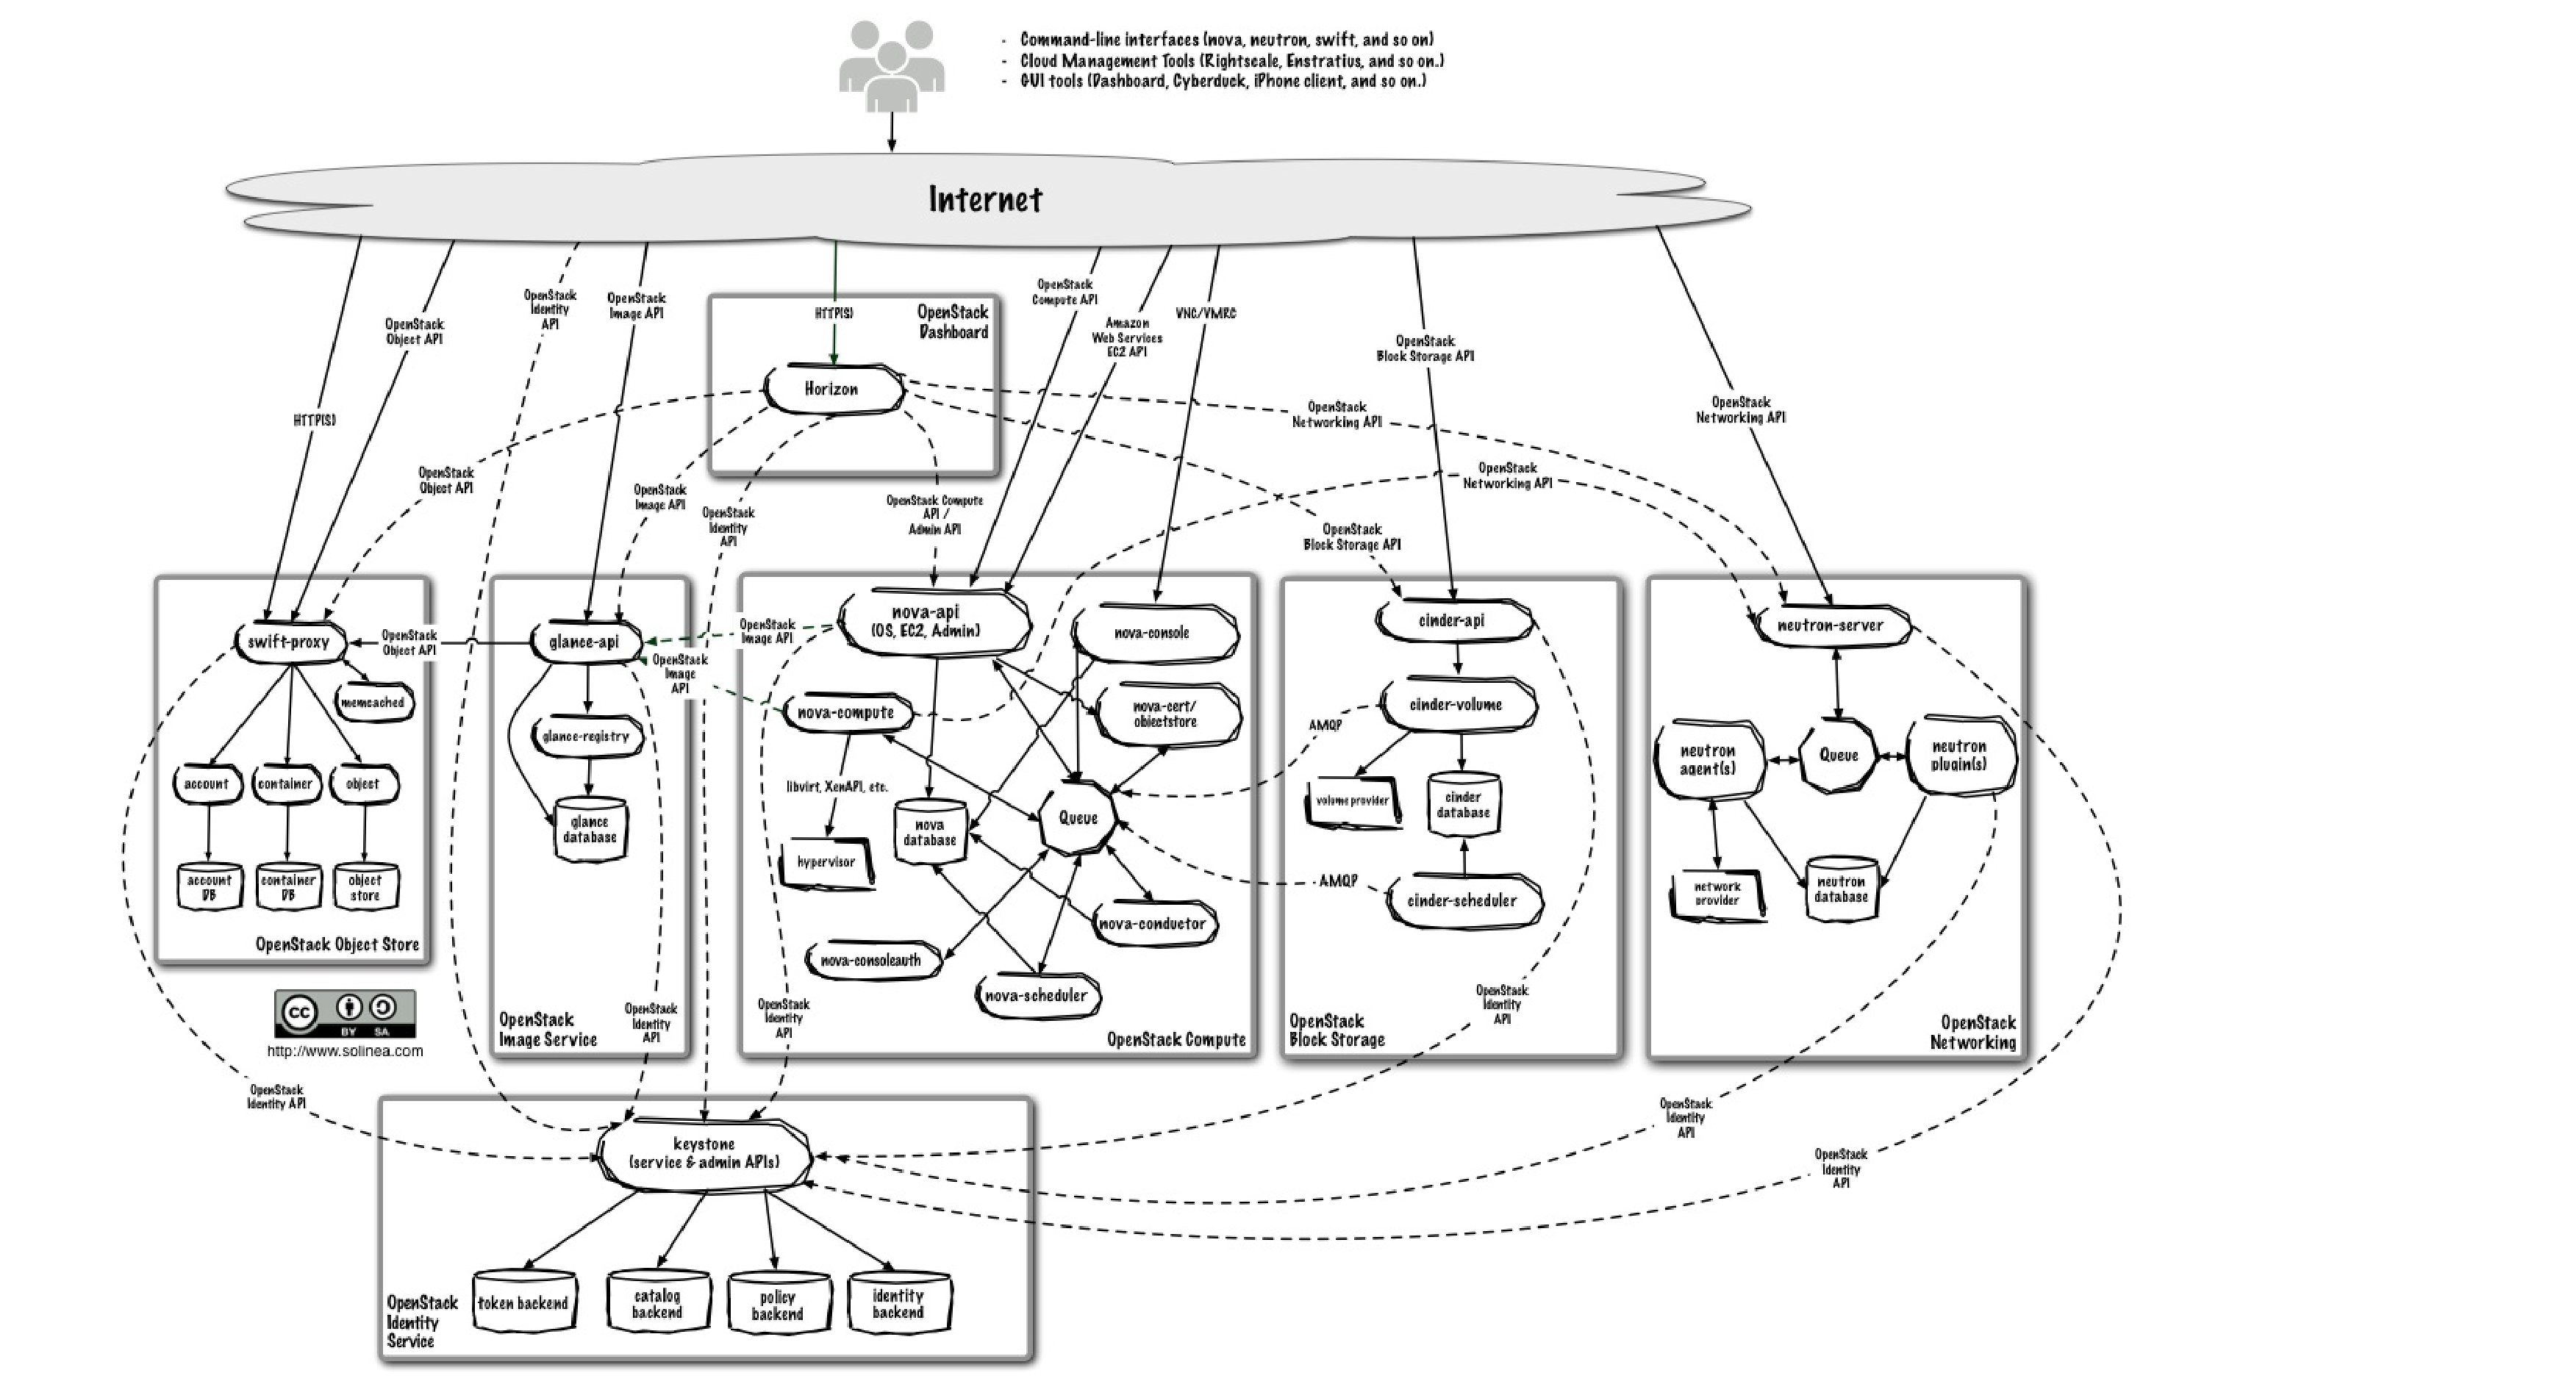
\includegraphics[height=3cm,
    angle=0]{./images/OpenStack_structure.eps}}
  \caption{Restitution curve
  \footnote{\url{http://www.physio.unibe.ch/~kucera/group/projects.aspx}}}
  \label{fig:OpenStack_structure}
\end{figure} 


There are basically eleven components of OpenStack, each one offers an API that
facilitates this integration.
\begin{enumerate}
  \item service Dashboard: project Horizon
  \item service Compute: project Nova
  \item service Networking: project Neutron
  \item service Object Storage: project Swift
  \item service Block Storage: project Cinder
  \item service Identity: project Keystone
  \item service Telemetry: project Ceilometer
  \item service Orchestration (automated arrangement, coordination, and
  management of complex computer systems, middleware, and services): project Heat
  
  Canonical use project Juju on Ubuntu O/S. Juju allows you to instantly deploy,
  integrate and scale your IT stack/services/applications.
  
  \item service Database Service: project Trove
\end{enumerate}

\section{Versions}

OpenStack releases are numbered YYYY.N time-based scheme, e.g. the second
release in 2012 will be 2012.2. There are also codename to identify the release,
with order alphabetically, e.g. Juno = the 10-th release so far. 
\url{https://wiki.openstack.org/wiki/Release_Naming}

\subsection{Austin}

\subsection{Bexar}

\subsection{Cactus}

\subsection{Diablo}

\subsection{Essex}

\subsection{Folsom}

\subsection{Grizzly}

\subsection{Havana}

\subsection{Icehouse}

\subsection{Juno}

OpenStack 2014.2 is Juno, the 10th release with 342 new features to support
\url{https://wiki.openstack.org/wiki/ReleaseNotes/Juno}
\begin{itemize}
  \item software development
  \item big data analysis
  \item application infrastructure at scale
\end{itemize}

\url{http://www.openstack.org/software/juno/}
\subsection{Kilo}


\section{host O/S}
\label{sec:OpenStack_host-OS}

Ubuntu is currently the most popular host O/S for OpenStack.
\footnote{\url{http://www.zdnet.com/article/openstacks-top-operating-system-ubuntu-linux/}}

To minimize clutter and provide more resources for OpenStack, we recommend a
minimal installation of your Linux distribution, with a 64-bit version on at
least the compute node (otherwise, we can not run 64-bit server instances of
guest O/S).
\url{http://docs.openstack.org/juno/install-guide/install/apt/content/ch_basic_environment.html}

You can install on a virtual machine, i.e. nested VM
(Sect.\ref{sec:OpenStack_single-node}), or a cluster
(Sect.\ref{sec:OpenStack_cluster}). OpenStack requires Ubuntu Server
\url{https://ask.openstack.org/en/question/4882/how-can-i-install-openstack-on-ubuntu-1204-desktop/}.
If we need the UI, we can install the UI later on Ubuntu Server.


\subsection{Cluster}
\label{sec:OpenStack_cluster}

The minimum amount of server is 7 with 2 disks, two of which have 2 NIC's.
Another option is to use Virtual MAAS.
\url{http://www.ubuntu.com/download/cloud/install-ubuntu-openstack}

\subsection{Single node}
\label{sec:OpenStack_single-node}

Ubuntu 12.04 running on Oracle VirtualBox with two NIC's.

\url{http://ilearnstack.com/2013/04/26/setting-up-a-single-node-openstack-environment/}




\chapter{OSv}
\label{chap:OSv}

\url{http://osv.io/}

OSv is the open source operating system designed for the cloud.
\chapter{Cloud Runtime Environment: Google App Engine}
\label{chap:AppEngine}

An App Engine application is an application that can run on Google Cloud
Platform, which include Linux-based VM instances. The application must be
written in one of the following languages
\begin{itemize}
  \item Java (use Java Runtime Environment)
  \item Python (use fast Python interpreter and standard Python libraries)
  \item PHP
  \item Go (use Go Runtime Environment)
\end{itemize}
\url{https://cloud.google.com/appengine/docs/whatisgoogleappengine}

App Engine gives you 1 GB of data storage and traffic for free, which can be
increased by enabling paid applications.

When your App Engine application is running in the cloud, Google provides a
scalable number of instances of your app's modules. Each instance runs in its
own hosting environment. Initially, it is a sandbox,
Fig.\ref{fig:GoogleCloudPlatform_environment}, containing your code, a webserver
and a language runtime. The language runtime thus was modified to enforce the
sandbox constraints, disabling some of the language APIs (e.g. access
filesystem). Later, Google supports running on Virtual Machine (Managed VM), and
is not restricted to Java and Python runtime environments, e.g. Go runtime
environment or custom runtime
\url{https://cloud.google.com/appengine/docs/managed-vms/custom-runtimes} as
your application is packaged as a Docker container.
When these runtimes are deployed in a Managed VM hosting environment, they support the following service APIs:
\begin{verbatim}
Datastore
Memcache 
Task Queues
Logging
Users
\end{verbatim}

You can also add third-party libraries and frameworks to your app.

You use the existing \verb!app.yaml! (for Python), \verb!appengine-web.xml!
configuration files (for PHP), and App Engine SDK tools to develop and deploy
applications to Managed VMs.

\section{Writing Python apps}

We need \verb!app.yaml! file. For more information, read the Python manual book 
(chapter on Web Framework for Python).

\section{Writing PHP apps}

we need \verb!appengine-web.xml! file. 

\begin{figure}[hbt]
  \centerline{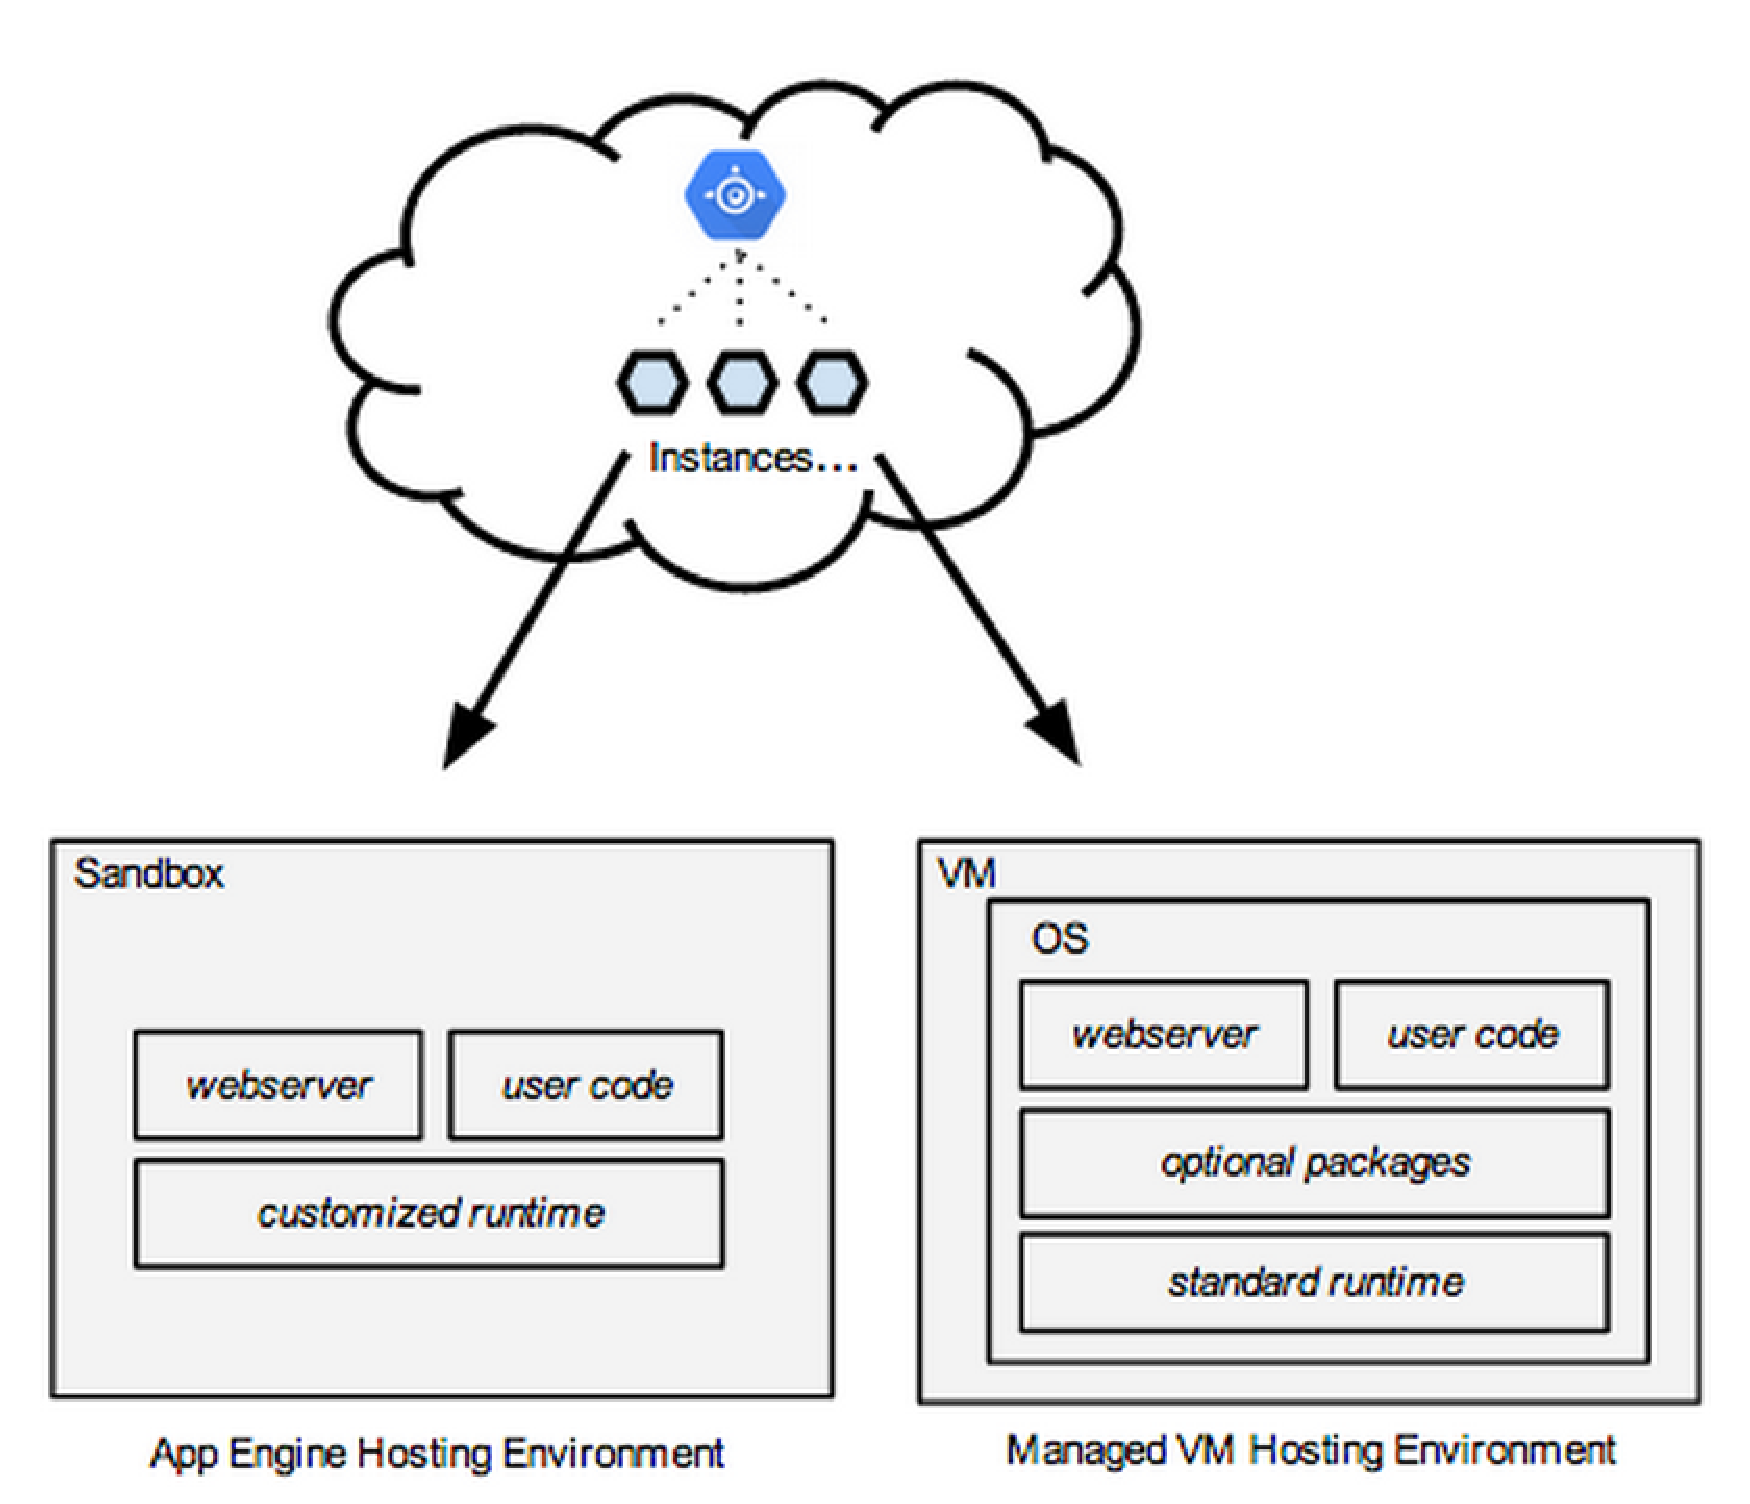
\includegraphics[height=3cm,
    angle=0]{./images/GoogleCloudPlatform_environment.eps}}
  \caption{}
  \label{fig:GoogleCloudPlatform_environment}
\end{figure}


\section{Test your application}

The Launcher is an application for creating, running, uploading, and otherwise
managing Google App Engine applications. 
\url{https://code.google.com/p/google-appengine-wx-launcher/}

\section{Container-as-a-Service}

 The rise of containers and Kubernetes shifted the focus to Containers as a Service (CaaS) from traditional infrastructure services, IaaS. 
 





\import*{../Sys_admin/}{Hyperscale_computing.tex}

\part{Tools to Interact with a Cloud Machine}
\import*{../Python_Manual/}{Cloud_PythonPackages.tex}

%\part{Search}
\part{Search Engines}
\chapter{Information Retrieval}
\label{chap:Information_Retrieval}

Information retrieval (IR) is an activity to extract information relevant to a
given information from a collection of information resources. The search can be based
on {\it metadata} or full-text (or other content-based) indexing. When the data
is huge, {\bf automated information retrieval} is important.

The idea of using computer to do IR started as early as 1945, from an article
``As We May Think'' by Vannevar Bush. The first automated IR was built in 1950s
and 1960s. Web-search engine is a form of very-large scale IR applications.

To do automated IR, the documents are often transformed or represented in some
form. This is called a model and is categorized according to 2 dimensions: {\it
mathematical basis} and the {\it properties of the model},
Fig.\ref{fig:IR_classification}.

\begin{figure}[hbt]
  \centerline{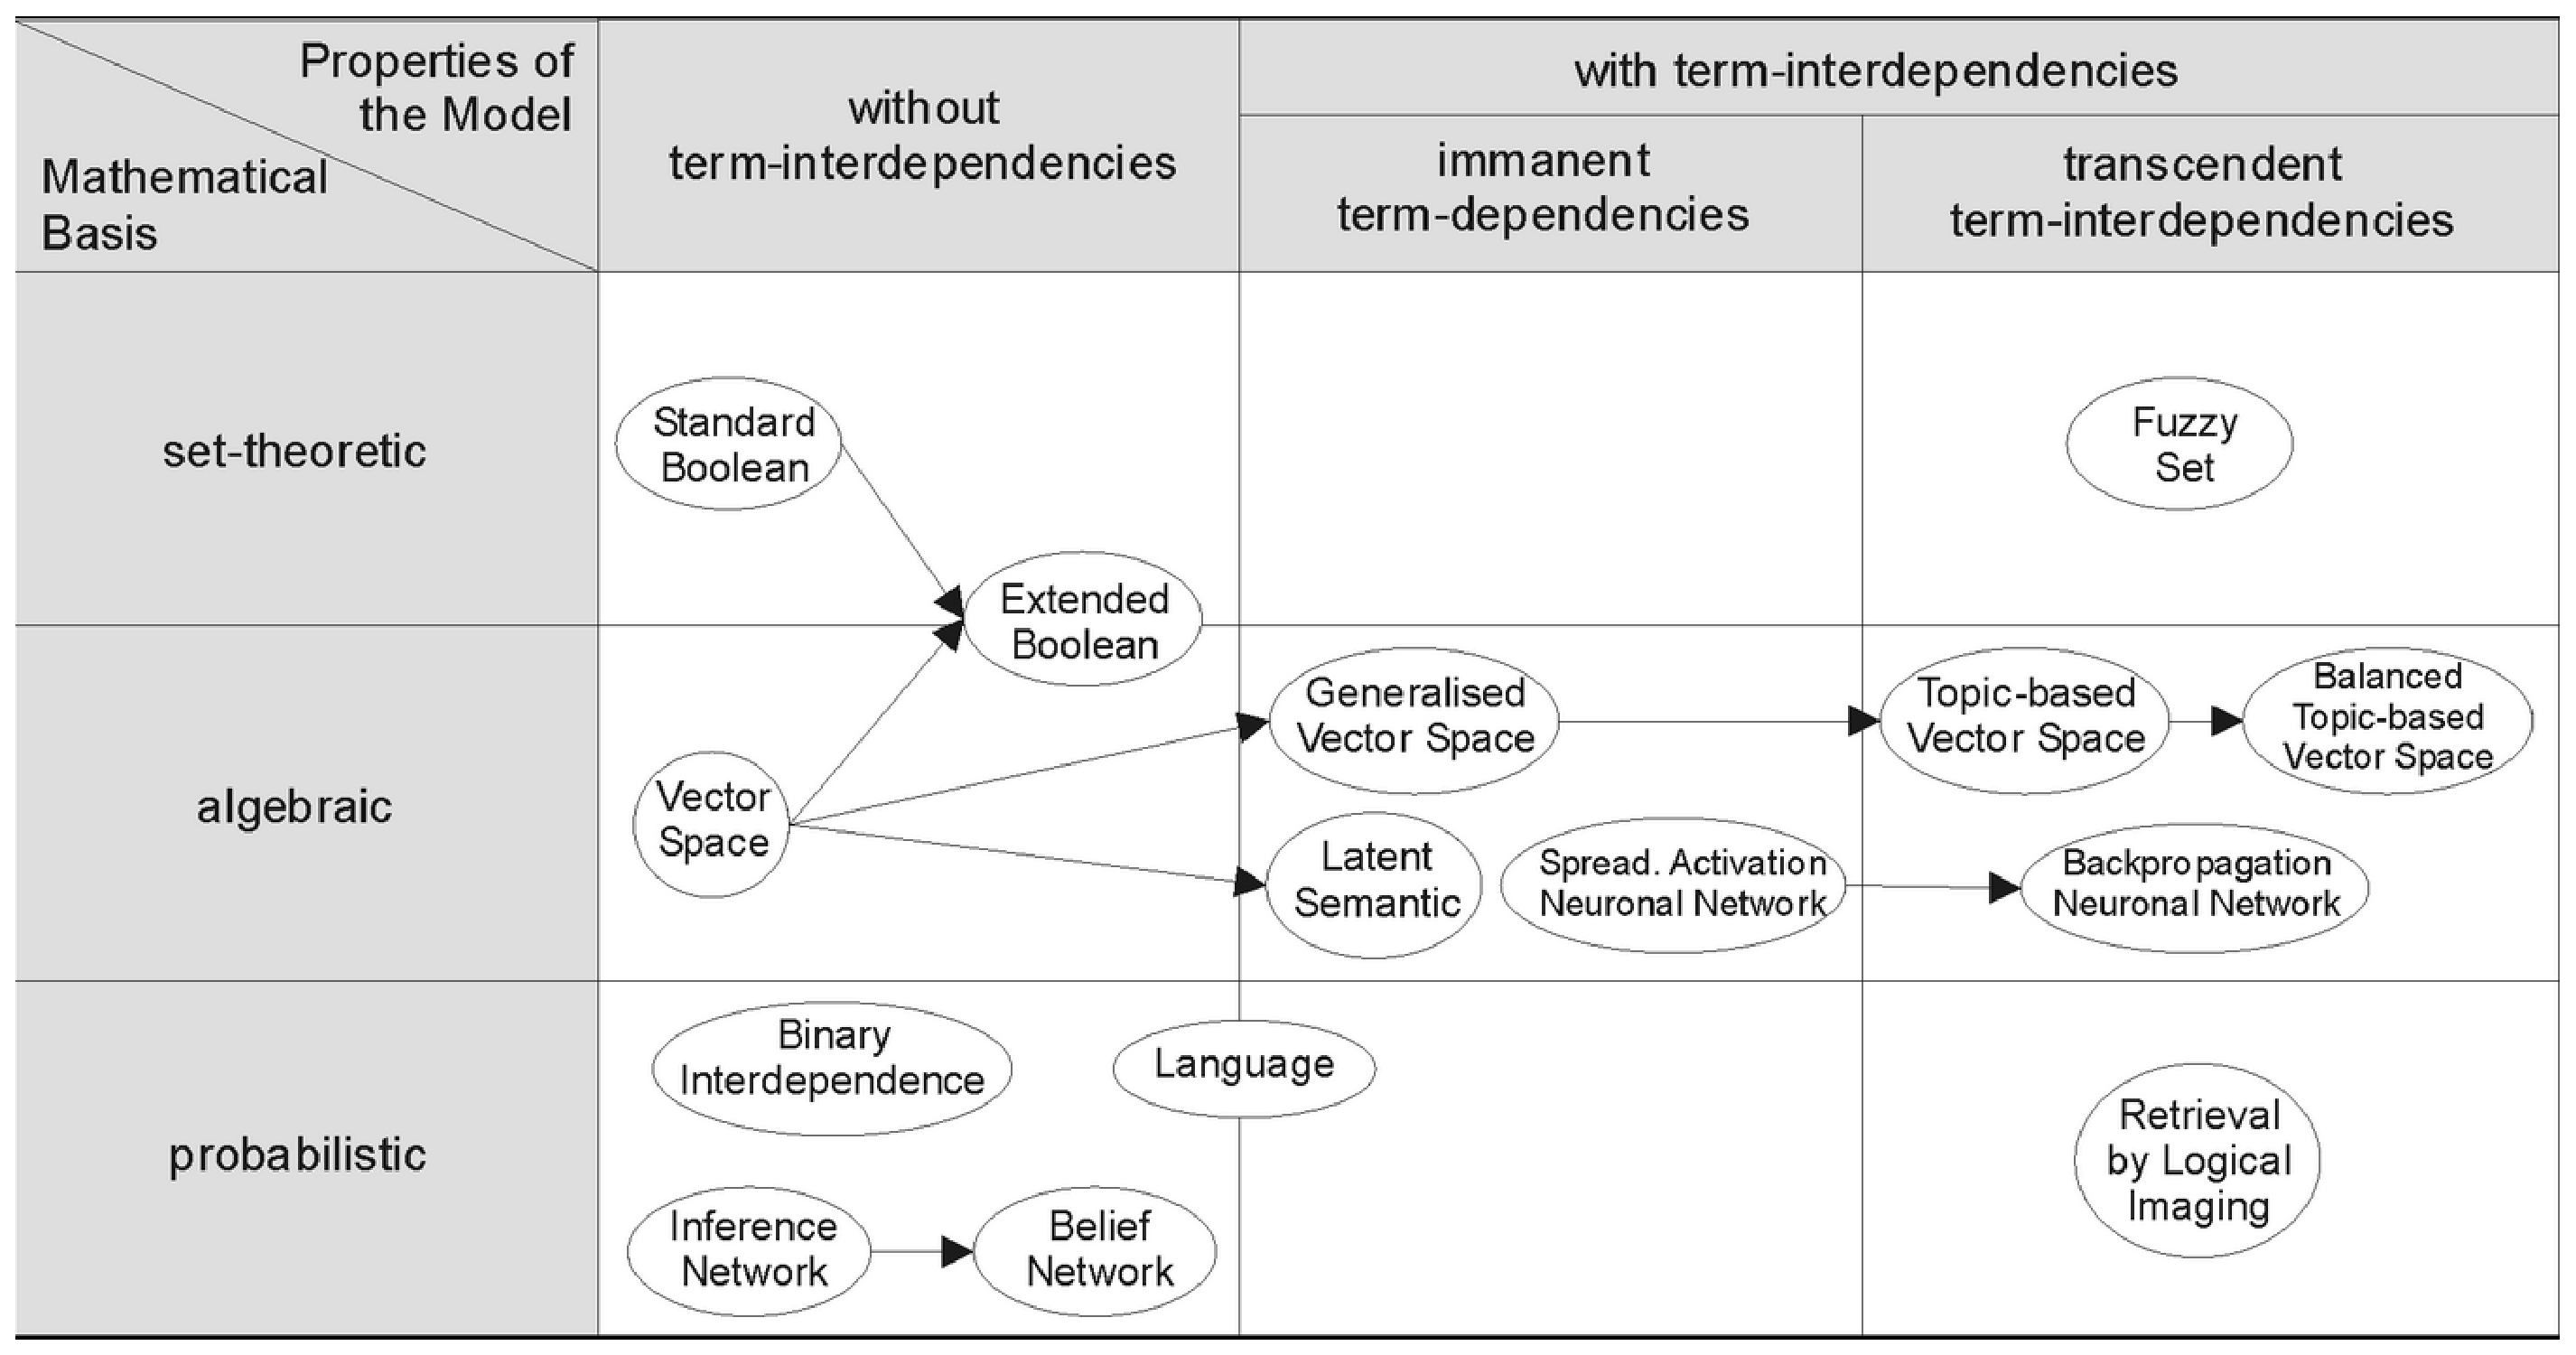
\includegraphics[height=5cm,
    angle=0]{./images/IR_classification.eps}}
\caption{Categorization of IR-models}
\label{fig:IR_classification}
\end{figure}


Libraries to do IR
\begin{enumerate}
  \item ElasticSearch (Chap.\ref{chap:elastic_search})
  \item Lemur 
  \item Lucene (Sect.\ref{sec:Lucene})
  \item Solr (Chap.\ref{chap:Solr})
  \item Sphinx
  \item Xapian
  \item Terrier Search Engine
\end{enumerate}
\url{http://en.wikipedia.org/wiki/List_of_information_retrieval_libraries}
\chapter{Desktop Search Engines}
\label{chap:Desktop_SearchEngine}

\url{http://en.wikipedia.org/wiki/List_of_search_engines\#Desktop_search_engines}

\section{Google Desktop}
\label{sec:Google_Desktop}

Google Desktop is a discontinued product, due to the huge shift from local to
cloud-based storage and computing, as well as the integration of search and
gadget functionality into the modern operating system (O/S).
\begin{enumerate}
  \item Email messages
  \item Computer files
  \item Music
  \item Photos
  \item Chats
  \item Web pages viewed
  \item Google gadget on user's desktop sidebar of Windows
\end{enumerate}

To display on Linux's desktop sidebar, use
\url{https://code.google.com/p/google-gadgets-for-linux/}

\section{DocFetcher}
\label{sec:DocFetcher}

DocFetcher is open-source multi-platform, written in Java with standard Widget
Toolkit for GUI. The searching and indexing capabilities of DocFetcher is based
on Apache Lucene (Sect.\ref{sec:Lucene}).

It can parse text from documents in
\begin{enumerate}
  \item formats: PDF, HTML, EPUB, MS Office, OpenOffice
  \item zip file: zip, 7z, rar, tar.*
  \item Outlook emails: PST files
  \item customized to search in any kind of source-code files
\end{enumerate}
It also 
\begin{itemize}
  \item automatically updates the indexes (when files are modified)
  \item feature to exclude files from being indexed using regular expressions
\end{itemize}


\url{http://en.wikipedia.org/wiki/DocFetcher}

\section{Find and Run Robot}
\chapter{Web Search Engines}
\label{chap:Web_SearchEngines}

\url{http://en.wikipedia.org/wiki/List_of_search_engines}

Building Internet-scale search engines requires huge amounts of data and
therefore large numbers of machines to process it. Mike Cafarella and Doug
Cutting estimated a system supporting a 1-billion-page index would cost around
half a million dollars in hardware, with a monthly running cost of \$30,000.


Yahoo! Search consists of four primary components
\begin{enumerate}
  \item Crawler: download the pages (from web servers) - Chap.\ref{chap:WebCrawling}
  
  \item WebMap: build a (huge) graphs of this known web (i.e. the linking
  between pages)
  
  The graph being built for the Internet can reach $10^{12}$ edges (each
  representing a web link), and $10^{11}$ nodes (each representing a distinct
  URL).  Creating and analyzing such a large graph requires a large number of
  computers running for many days. 
  
  \item Indexer: build a reverse index to the best pages
  \item Runtime: answer uer's queries.
\end{enumerate}

\section{Nutch (web search engine + web crawler)}
\label{sec:Nutch_websearch_engine}

Nutch is an open-source web search engine based on Lucene
(Sect.\ref{sec:Lucene}) by two authors (Doug Cutting, Mike Cafarella).
The fetcher ("robot" or "web crawler") has been written from scratch
specifically for this project. However, they soon realized that their
architecture wouldn't scale to the billions of pages on the Web when they
started in 2002. Then, when a paper describing Google's Distributed FS called
GFS was published in 2003.

GFS, or something like it, would solve their storage needs for the very large
files generated as a part of the web crawl and indexing process. In particular,
GFS would free up time being spent on administrative tasks such as managing
storage nodes. In 2004, they set about writing an open source implementation,
the Nutch Distributed Filesystem (NDFS).   

Again, with the paper describing MapReduce programming model from Google
(Sect.\ref{sec:MapReduce}), Nutch added an implementation for MapReduce
programming model and porting the existing algorithm from Nutch to using
MapReduce and NDFS.


\section{Bing Search API}

We can use the results returned by Bing Search API.
Microsoft provides RESTful APIs which can be accessed from PHP, Microsoft .NET
and C\#, or wrappers in Python (bingpy - Sect.\ref{sec:bingpy}).


\subsection{BingPy}
\label{sec:bingpy}

\url{https://pypi.python.org/pypi/bingpy/0.0.1}

\begin{verbatim}
from bingpy import WebSearch
web = WebSearch("YOUR_API_KEY")
pages = web.search("kyoto", 20)
for page in pages:
    print page.title
\end{verbatim}

Bing key or account key are used by applications to access your Microsoft Azure
Marketplace dataset subscriptions. Do not share your account keys with other users.

To get Bing Key: \url{http://www.articlekevo.com/get-bing-api-key/}
% :
% \begin{enumerate}
%   \item A distributed file system (Hadoop Distributed File System -
%   Sect.\ref{sec:HadoopFS})
%     
%   \item A MapReduce facility which become Apache Hadoop project.
% \end{enumerate}

\chapter{Solr}
\label{chap:Solr}

Solr is the descendant of {\bf Lucene}, a search indexer for information
retrieval (Sect.\ref{sec:Lucene}). Perhaps the most significant deployment of
Lucene is Wikipedia, where it powers search for the entire site.

\section{Lucene (information retrieval)}
\label{sec:Lucene}


Lucene is an open-source {\it information retrieval} software library
(Chap.\ref{chap:Information_Retrieval}), initially written in Java. It has been
ported to  Delphi, Perl, C\#, C++, Python, Ruby, and PHP.

While suitable for any applications that require {\it full-text indexing} and
searching capability, Lucene has been widely used mainly in implementation of
{\bf Internet search engines} and local, single-site searching. 

A single document is represented as {\bf fields} of text. So, the APIs of Lucene
is independent of the file format. It can accepts text from PDF, HTML, MS Word,
OpenDocuments and many others (as long as the textual information can be
extracted); but \textcolor{red}{not images}.

Lucene needs user to feed the data into the system. So, it doesn't do crawling
and HTML parsing. There are other projects that use Lucene and add these
features.
\begin{enumerate}
  \item Apache Nutch: web crawling and HTML parsing
  \item Apache Solr: enterprise search server (Sect.\ref{sec:Solr})
  \item Elasticsearch: enterprise search server (Chap.\ref{chap:elastic_search})
  \item DocFetcher: multi-platform desktop search application
  (Sect.\ref{sec:DocFetcher})
  \item 
\end{enumerate}

Similar tools (NOTE: Lucene is written in Java)
\begin{enumerate}
  \item Lucene.NET: .NET framework
  \item Ferret: Ruby language, and use Poshlib
  \item Kinosearch: Perl and C
  \item Apache Lucy: the successor of Ferret and Kinosearch, with bindings to
  both Perl and Ruby.
\end{enumerate}

A GUI to Lucene is 
\begin{enumerate}
  \item {\bf Luke}: Java-based GUI (display and modify indexes)
\end{enumerate}

Companies that use Lucene
\begin{enumerate}
  \item Twitter: real-time search
\end{enumerate}

\section{Solr}
\label{sec:Solr}

Solr was created in 2004 at CNET Networks as an in-house project to add search
capability for the company website. Every new open-source project need to go
through an incubation period to ensure the open-source is legal; when it
passes, it is graduated. Solr started the incubation period in Jan, 2006 and
graduated in Jan, 2007.

Derived from Lucene (Sect.\ref{sec:Lucene}), Solr enables the search and
indexing as  a {\it search platform} for being used in an enterprise.
Solr is highly scalable, with support for NoSQL features (Sect.\ref{sec:NoSQL}).
It also includes full-text search, hit highlighting, faceted search, dynamic
clustering, database integration, and rich document (e.g., Word, PDF) handling.
Solr's powerful external configuration allows it to be tailored to many types of
application without Java coding, and it has a plugin architecture to support
more advanced customization.

Solr uses the Lucene Java search library at its core for full-text indexing and
search, and has REST-like HTTP/XML and JSON APIs that make it usable from most
popular programming languages.

\begin{enumerate}
  \item Solr 1.3 (2008, Sept): distributed search capabilities and performance
  enhancements 
  \item Solr 1.4 (2008, Nov): nhancements in indexing, searching and faceting
  along with many other improvements such as Rich Document processing (PDF,
  Word, HTML), Search Results clustering based on Carrot2 (Sect.\ref{sec:Carrot})
  and also improved database integration. The release also features many additional plug-ins   
  
  \item 2010, March: Solr and Lucene merged
  \item Solr 3.1 (2011): version scheme changed to match with Lucene
  \item Solr 4.0 (2012, Oct): new SolrCloud feature
  \item Solr 4.1, 4.2, 4.2.1
\end{enumerate}


\section{Carrot2}
\label{sec:Carrot}

Carrot is an open-source search result clustering engine.
Carrot$^2$ offers ready-to-use components for fetching search results from
various sources.

Typically, it fetch search results from an external search engine
\begin{verbatim}
Bing search API
PubMed
Lucene index
OpenSearch
Solr server
Generic XML files
eTools metasearch
\end{verbatim}
Lucene / Solr index or load text files from a local disk. We can add support for
others using code examples provided.

\chapter{ElasticSearch}
\label{chap:elastic_search}

\section{Introductrion}

ElasticSearch is a search server that use Lucene
(Sect.\ref{sec:Lucene}) as the back-end. Lucene does indexing the given input,
but it does not do crawling, and ElasticSearch incorporate the crawling feature
into it.

\subsection{0.5.0}

\url{https://www.elastic.co/downloads/past-releases/elasticsearch-0-5-0}

\begin{verbatim}
aopalliance-1.0.jar
elasticsearch-0.5.0.jar
google-collections-1.0.jar
guice-2.0.jar
guice-assisted-inject-2.0.jar
guice-multibindings-2.0.jar
jackson-core-asl-1.4.2.jar
jackson-mapper-asl-1.4.2.jar
jgroups-2.9.0.GA.jar
jline-0.9.94.jar
joda-time-1.6.jar
log4j-1.2.15.jar
flucene-analyzers-3.0.1.jar
lucene-core-3.0.1.jar
lucene-queries-3.0.1.jar
netty-3.1.5.GA.jar
slf4j-api-1.5.8.jar
slf4j-log4j12-1.5.8.jar
\end{verbatim}



\section{Marvel plugin}

Marvel is a plugin for Elasticsearch that helps to provide statistics of the nodes activities
in the ElasticSearch cluster.

\url{http://www.elasticsearch.com/products/marvel/?_ga=1.97357526.87852203.1421369435}

\section{Elasticsearch Puppet module}

Elasticsearch Puppet module 0.4.0 supports multiple instances of Elasticsearch running on a single machine.
\url{https://www.elastic.co/blog/elasticsearch-puppet-module-0-4-0-released}

\section{Elasticsearch on Microsoft Azure}

\url{https://www.nuget.org/packages/Microsoft.Experimental.Azure.ElasticSearch/0.4.0-alpha}
 

\part{Web Crawling}
\chapter{Web Crawling}
\label{chap:WebCrawling}

\section{Introduction}


\subsection{screen scraping}
\label{sec:screen_scrapping}

Originally, screen scrapping refers to the practice of reading text data from
the terminal's screen, by reading the terminal's memory through its auxiliary
port. UI from that area were often simply text-based dumped terminals.
The screen scraper might connect to the legacy system via Telnet, emulate the
keystrokes needed to navigate the old user interface, process the resulting
display output, extract the desired data, and pass it on to the modern system.




\subsection{web scraping}
\label{sec:web_scrapping}

Even though web pages (built from HTML, XHTML) requently contain a wealth of useful data in text form, most have been designed for human end-users, and not for ease of automated use.
Several tools to scrape web content (known as {\bf web scraper}) have been developed.
A web scraper provides APIs to extract data from a web site.

Newer forms of web scraping involve listening to data feeds from web servers, e.g. feeds in JSON format.
Recently, these scrapers rely on using techniques in DOM parsing, computer vision and natural language processing
that can simulate human processing that occurs when reading a webpage, to automatically extract useful information.

\subsection{Tools}

Scrapy (Python-based tool - Sect.\ref{sec:Scrapy}) which is faster than
Mechanize but not as scalable as Nutch (Chap.\ref{chap:Nutch}) or Heritrix,
which means that it's not meant to be used for crawling the entire web, but it's
OK for crawling a lot (5000+) of sites, even huge ones like Amazon.



\section{Scrapy (Python-based)}
\label{sec:Scrapy}

So you need to extract some information from a website, but the website doesn't
provide any API or mechanism to access that info programmatically. Scrapy can
help you extract that information.

Scrapy is an application framework for crawling web sites and extracting
structured data which can be used for a wide range of useful applications, like
data mining, information processing or historical archival.


We should read this in Python manual book.


\section{Crawler4j (Java-based)}

You can setup a multi-threaded web crawler in few minutes.

A crawler is a class extend from \verb!WebCrawler! class, with 3 informations need to be provided
\begin{enumerate}
  \item the pattern
  \item override \verb!shoudVisit()! method: decides whether the given URL should be crawled or not.
  \item override \verb!visit()! method: is called after the content of a URL is downloaded successfull. What it does is
  to extract the right information you want ( url, text, links, html, and unique id of the downloaded page)
\end{enumerate}

A controller class is also required, from which you provide the seed URLs.

Other settings:
\begin{enumerate}
  \item depth of search: \verb!crawlConfig.setMaxDepthOfCrawling(maxDepthOfCrawling);!
  
  \item max number of pages to crawl: \verb!crawlConfig.setMaxPagesToFetch(maxPagesToFetch);!
  
  \item politeness, i.e. how often to request a page to a website (default: 200 ms): \verb!crawlConfig.setPolitenessDelay(politenessDelay);!
  
  \item run behind proxy or not?
  
  \item resume crawling or not?
  
  \item agent string: a user agent strings identify what a client (e.g. a web browser, a crawler) is using to access a web-page.
  
  \url{http://whatsmyuseragent.com/WhatsAUserAgent}
\end{enumerate}

\begin{verbatim}
public class MyCrawler extends WebCrawler {

    private final static Pattern FILTERS = Pattern.compile(".*(\\.(css|js|gif|jpg"
                                                           + "|png|mp3|mp3|zip|gz))$");
                                                           
                                                           
\end{verbatim}
\url{https://github.com/yasserg/crawler4j}
\chapter{Apache Nutch}
\label{chap:Apache_Nutch}
\label{chap:Nutch}

Sect.\ref{sec:Nutch_websearch_engine} describe how Apache Nutch can be used as a web search engine.
In this chapter, we will discuss how Nutch can be used as a web crawler (Chap.\ref{chap:WebCrawling}).



\part{Document Management}
\chapter{Social Intranet: Document Management}

Enterprise social networks (Chatter, Yammer, Socialcast, Jive). Microsoft has
SkyeDrive, but the social component in SharePoint is very weak. Thus, Microsoft
later bought Yammer (Sect.\ref{sec:Yammer}).

Perhaps the two most famous brands in the history of enterprise software, Lotus
and SharePoint, will soon disappear. We mean brands, not specific products.
Because by renaming their products, vendors try to erase the association with
outdated technologies in customer brain. 

\section{OpenKM (open-source)}
\label{sec:OpenKM}

OpenKM is a web base document management application that uses standards and Open Source technologies.

OpenKM provides full document management capabilities including version control
and file history, metadata, scanning, workflow, search, and more.
The social activities around the content connect people to other people,
information to information, and people to information; helping to manage, more
efficiently, the collective intelligence of the human resources of the company.

While not quite as polished as some of the other open-source document management
systems, OpenKM also offers enterprise-ready capabilities. Key features include
drag-and-drop functionality, a powerful search engine, and tag clouds. Operating
System: OS Independent.

OpenKM Replaces: Documentum, Microsoft SharePoint, OpenText


OpenKM provides free features (Community version), and commercial features (Professional version):
\url{http://wiki.openkm.com/index.php/User_Guide}

\section{Nuxeo (open-source)}
\label{sec:Nuxeo}

Alfresco vs Nuxeo vs OpenKM:
\url{http://www.slideshare.net/nuxeo/comparing-the-code-quality-of-ecms}

\section{Epiware (open-source)}
\label{sec:EpiWare}



\section{Yammer (social intranet)}
\label{sec:Yammer}

Yammer is revolutionizing internal corporate communications by bringing together
all of a company's employees inside a private and secure enterprise social
network.

Using Yammer is like using Facebook or Twitter, but it is an enterprise-class
software built from the ground up to drive business objectives.

Yammer was bought by Microsoft in 2012.
Microsoft bought Yammer not for the engine, but for the customer base and the
image of  social vendor.
In June 2013, Office 365 users got the opportunity to replace SharePoint
Newsfeed to Yammer, and Microsoft continues to insist that Yammer - is its
future and that soon Yammer will become the platform for all its business apps.
Yammer - is purely SaaS service (Sect.\ref{sec:SaaS}), and for the companies
that use local SharePoint server and aren't ready to move to SaaS, Newsfeed
remains the primary solution.


\section{SharePoint + SkyeDrive}
\label{sec:SharePoint}

Organizations use SharePoint to create websites. You can use it as a secure
place to store, organize, share, and access information from almost any device.
All you need is a web browser, such as Internet Explorer, Chrome, or Firefox.


SharePoint is not a front-end, but a back-end instead, which provides
\begin{itemize}
  \item framework for web app development
  
  \item multi-purpose platform allows for managing and provisioning of intranet portals, extranets and websites, document management and file management,
  
  \item collaboration spaces, social networking tools, enterprise search, business intelligence tooling
  
  \item process/information integration, and third-party developed solutions
\end{itemize}

SharePoint is a toolsuite with many products
\begin{enumerate}
  \item SharePoint Online
  \item SharePoint Foundation
  \item SharePoint Server
  \item sharePoint Designer 2013
  \item OneDrive for Business folder sync: Desktop-app
\end{enumerate}
\url{https://support.office.com/en-za/article/What-is-SharePoint-97b915e6-651b-43b2-827d-fb25777f446f}

\url{http://blog.apterainc.com/bid/316563/What-is-Microsoft-SharePoint-Used-For}

\url{http://www.liventerprise.com/compare/OpenKM_vs_SharePoint/}

\section{IBM Lotus Notes}

Lotus appeared back in the 80-s years of last century. In 1995 IBM acquired
Lotus Development and began selling their products Lotus Notes/Domino. In the
following years most IBM collaboration systems moved under the Lotus umbrella.
But last year the revolution occurred. The last child of the Lotus family - SaaS
suite LotusLive was renamed to SmartCloud for Social Business. And then the name
Lotus was removed from other products. The final nail was the recent launch of
Notes/Domino 9.0 Social Edition (without Lotus).


\section{Dropbox for Enterprise}


\section{Chatter (Saleforce)}
\label{sec:Chatter}

With Chatter, it's easy to work together and know everything that's happening in your company.

\url{http://www.liventerprise.com/tool/Salesforce_Chatter/}


\section{Google Apps (web-based, internet-capable)}

Google Apps offer completely browser-based office applications like a word
processor and spreadsheet, as well as communication tools like chat and email,
as well as collaboration tools like project managers and wikis.

\section{Zoho's Office suites (web-based)}

Zoho offer completely browser-based office applications like a word processor
and spreadsheet, as well as communication tools like chat and email, as well as
collaboration tools like project managers and wikis.

\url{http://lifehacker.com/315256/zoho-suite-vs-google-docs}




\part{Database}
\chapter{Google Bigtable}
\label{chap:google_bigtable}

Unlike a table in a traditional relational database systems (MySQL, Oracle,
\ldots), the table in Bigtable is totally different. 
A table in Bigtable is a
sparse, distributed, persistent multidimensional sorted map, which is indexed by
a row key, column key, and a timestamp.
It is aka 
key-value store, a column-family-oriented database, and sometimes a database
storing versioned maps of maps.



 
\chapter{HBase}
\label{chap:HBase}

HBase is a distributed NoSQL database that stores data in HDFS
(Sect.\ref{sec:HadoopFS}). HBase operations do not use MapReduce (Apache Hive is
the one that use MapReduce - Chap.\ref{chap:Hive_PrestoDB}) and thus provides a real-time
data access. Use it when you need  random, realtime read/write access to your
Big Data. This project's goal is the hosting of very large tables -- billions of
rows X millions of columns -- atop clusters of commodity hardware. HBase is
developed based on Google Bigtable (Chap.\ref{chap:google_bigtable}).

Based on Eric Brewer's CAP theorem, HBase is a CP type system (Consistency,
Partition Tolerance). HBase isn't fully ACID compliant, although it does support
certain properties. \url{https://www.xplenty.com/blog/2014/05/hive-vs-hbase/}

\section{Concepts}

HBase's data model is in the form of tables, consisting of rows and columns.
However, the concept of table in HBase is totally different from that in
relational database systems (MySQL, Oracle, \ldots). The concept of rows and
columns are also different. 

HBase is very much a distributed database; and it is more a ``Data Store'' than
a ``Data Base''  as it lacks many features found in a RDBMS (e.g. typed
columns, secondary indexes, triggers, advanced query languages\ldots). Languages
to query data stored in HBase is discussed in Sect.\ref{sec:query-HBase}.


{\bf WHEN TO USE HBase?}
\begin{enumerate}
  \item the data must be extremely large

Even HDFS doesn't do well with anything less than 5 DataNodes.
  
  \item your data can live outside RDBMS
  
  An application built against an RDBMS cannot be "ported" to HBase by simply
  changing a JDBC driver, for example. Consider moving from an RDBMS to HBase as
  a complete redesign as opposed to a port. 
  
\end{enumerate}


\url{http://hbase.apache.org/book/architecture.html}

\begin{enumerate}
  \item Table names are Strings and composed
of characters that are safe for use in a file system path.

  \item Row: Within a table, data is stored according to its row. Rows are identified
uniquely by their row key. Row keys do not have a data type and are always
treated as a byte[ ] (byte array).

Row keys are the equivalent of primary keys in relational
database tables. You cannot choose to change which column in an HBase table will
be the row key after the table has been set up

  \item Column Family: Data within a row is grouped by column family. Column
families also impact the physical arrangement of data stored in HBase. For this
reason, \textcolor{red}{they must be defined up front and are not easily
modified}.


Every row in a table has the same column families, although a row need not store
data in all its families. Column families are Strings and composed of characters that are safe
for use in a file system path.


  \item Column Qualifier: Data within a column family is addressed via its column
qualifier, or simply, column. Column qualifiers need not be specified in advance.


Column qualifiers need not be consistent between rows. Like row keys, column
qualifiers do not have a data type and are always treated as a byte[ ].

  \item Cell: A combination of row key, column family, and column qualifier uniquely
identifies a cell. The data stored in a cell is referred to as that cell's value. Values
also do not have a data type and are always treated as a byte[ ].

  \item Timestamp: Values within a cell are versioned. Versions are identified by their
version number, which by default is the timestamp of when the cell was written.
If a timestamp is not specified during a write, the current timestamp is used. If
the timestamp is not specified for a read, the latest one is returned. The number
of cell value versions retained by HBase is configured for each column family.
The default number of cell versions is three. 
\end{enumerate}

there are various ways of describing this data model. You can
view the same thing as if it's a key-value store, where the key
is the row key and the value is the rest of the data in a column.
You can also consider
HBase to be a key-value store where the key is defined as row key, column family,
column qualifier, timestamp, and the value is the actual data stored in the cell.

\textcolor{red}{In HBase, Key is
formed by [row key, column family, column qualifier, timestamp] and Value is the
contents of the cell.}

\section{Design a HBase table}

Designing HBase tables
can be defined as answering the following questions in the context of a use case:
\begin{verbatim}
1.	What should the row key structure be and what should it contain?
2.	How many column families should the table have?
3.	What data goes into what column family?
4.	How many columns are in each column family?
5.	What should the column names be? Although column names don't need to be
defined on table creation, you need to know them when you write or read data.
6.	What information should go into the cells?
7.	How many versions should be stored for each cell?
\end{verbatim}
In
order to define that effectively, it is important to define the access patterns (read
as well as write) up front



\section{Cluster structure for HBase}


Make sure that user name of all machines and the path where the hbase is
installed are same in all machines. There are 3 types of nodes
\begin{enumerate}
  \item HBase Master:  responsible for assigning regions to HbaseRegionserver,
  monitors the health of each HbaseRegionserver
  
  \item ZooKeeper: a centralized service for maintaining configuration
  information, naming, providing        distributed synchronization, and providing group services.
  
  \item HBase RegionServer:  responsible for handling client read and write
  requests. It communicates with the Hbasemaster to get a list of regions to serve and to tell the master that it is alive.
\end{enumerate}
We can configure one machine in the cluster is designated as Hbase master and
Zookeeper. These master processes may be collocated with the Hadoop NameNode and
ResourceManager (oldname: JobTracker) for small clusters.

\section{Install}  

You can either (1) downloaded the pre-compiled version, or (2) compile from
source. 

\subsection{Pre-built}

The pre-compiled version can be downloaded from
\url{http://www.apache.org/dyn/closer.cgi/hbase/}.
The latest version is 0.99.1 (Oct-2014) which is a "developer preview" release.

\subsection{Build from source}

It is more complicated when you build from source. I will walk through the
complexity behind building HBase. From HBase 0.96, the project is split into
multiple modules
\begin{verbatim}
hbase-annotations
hbase-assembly
hbase-checkstyle
hbase-client
hbase-common
hbase-examples
hbase-hadoop1-compat
hbase-hadoop2-compat
hbase-hadoop-compat
hbase-it
hbase-prefix-tree
hbase-protocol
hbase-rest
hbase-server
hbase-shell
hbase-testing-util
hbase-thrift
\end{verbatim}

With HBase 0.98.8, the default Hadoop 2 is 2.2.0. If you have Hadoop 2.5.2, you
need to modify pom.xml to use the new default Hadoop version.

First, you need to have Hadoop installed with HDFS (Chap.\ref{chap:Hadoop}) and
Java configured (Sect.\ref{sec:configure_Java}). Then, you can try with the
following command
\begin{verbatim}
mvn clean install
mvn clean install -DskipTests
\end{verbatim}
The problem is that \verb!Hbase-rest! requires root privilege to create some
folder (Sect.\ref{sec:Hbase-rest-test}). However, when we use \verb!sudo!, the
compiled modules are stored in the \verb!/root/.m2/repository!, instead of your current user home directory.

\begin{verbatim}
sudo mvn clean install
sudo mvn clean install -DskipTests
\end{verbatim}
If you're succeed, it will generate HBase artifacts and Maven POM files and
install them int your local Maven repository \verb!~/.m2/repository!
(Troubleshoot: Sect.\ref{sec:troubleshoot_build}). 

Now we generate binary tarball to install on the cluster. 
\begin{verbatim}
mvn package
mvn assembly:single
\end{verbatim}
which creates
\begin{verbatim}
./target/hbase-0.98.8-yourversion.tar.gz
\end{verbatim}
Finally, copy the tarball that was generated in the last step to your cluster
and unpack them in the desired location, e.g. /usr/local/hbase-0.98.8.
\url{http://praveen.kumar.in/2011/06/20/building-hadoop-and-hbase-for-hbase-maven-application-development/}

IMPORTANT: We can do all of them in a single command
\begin{verbatim}
mvn -DskipTests clean install package assembly:single

mvn -DskipTests clean install package && mvn -DskipTests assembly:single
\end{verbatim}

If there is any error, try to build modules one by one
(Sect.\ref{sec:hbase_build_one-by-one}).

\subsection{HBase build module-by-module}
\label{sec:hbase_build_one-by-one}

Based on the pom.xml, the build order is
\begin{verbatim}
[INFO] HBase - Annotations
[INFO] HBase - Common
[INFO] HBase - Protocol
[INFO] HBase - Client  (depends annotations,common,protocol)
[INFO] HBase - Hadoop Two Compatibility (i.e. hbase-hadoop-compat)
[INFO] HBase - Prefix Tree (depends annotations,commmon,hadoop-compat)
[INFO] HBase - Server (depends annotations,common,protocol,client,hadoop-compat) 
[INFO] HBase - Testing Util (depends annotations,common,protocol,
                                 client,server,hadoop-compat)
[INFO] HBase - Thrift (depends annotations,common,protocol,client,
                                 server,hadoop-compat,testing-util,
                                 ${compat.module} which can be hadoop1-compat or
                                                               hadoop2-compat
                      )
[INFO] HBase - Rest   (depends annotations,common,protocol,client,
                                 server,hadoop-compat,testing-util,
                                 ${compat.module} which can be hadoop1-compat or
                                                               hadoop2-compat
                      )
[INFO] HBase - Shell  (depends annotations,common,protocol,client,
                                 server,hadoop-compat,testing-util,
                                 ${compat.module} which can be hadoop1-compat or
                                                               hadoop2-compat
                      )
[INFO] HBase - Integration Tests (it)
[INFO] HBase - Examples (depends annotations,common,protocol,client,
                                 server,hadoop-compat,testing-util, thrift,
                         )
[INFO] HBase - Assembly  (depends annotations,common,protocol,client,
                                 server,hadoop-compat,testing-util,
                                 it,
                                 ${compat.module} which can be hadoop1-compat or
                                                               hadoop2-compat
                         )
\end{verbatim}
and the build cycle is
\begin{verbatim}
[validate, initialize, generate-sources, process-sources, generate-resources,
process-resources, compile, process-classes, generate-test-sources, 
process-test-sources, generate-test-resources, process-test-resources, 
test-compile, process-test-classes, test, prepare-package, package, 
pre-integration-test, integration-test, post-integration-test, 
verify, install, deploy]
\end{verbatim}
The important stages are \verb!package!, \verb!install! and \verb!deploy!. We
try the first module \verb!hbase-annotations! and \verb!package! command
\begin{verbatim}
mvn -e install -pl hbase-annotations -e -X 2>&1 | tee
       ../mhbase-annotations.txt
mvn -e install -pl hbase-common -e -X 2>&1 | tee
       ../mhbase-common.txt
mvn -e install -pl hbase-protocol -e -X 2>&1 | tee
       ../mhbase-protocol.txt
mvn -e install -pl hbase-client -e -X 2>&1 | tee
       ../mhbase-client.txt
mvn -e install -pl hbase-hadoop-compat -e -X 2>&1 | tee
       ../mhbase-hadoop-compat.txt
mvn -e install -pl hbase-hadoop2-compat -e -X 2>&1 | tee
       ../mhbase-hadoop2-compat.txt
mvn -e install -pl hbase-prefix-tree -e -X 2>&1 | tee
       ../mhbase-prefix-tree.txt       
mvn -e install -pl hbase-server -e -X 2>&1 | tee
       ../mhbase-server.txt
       
\end{verbatim}
NOTE: Do not use parallel threads (e.g. -T 8) during debug.
Check the output error in \verb!../mhbase-annotations.txt! file.

If you success, the result will be copied to 
\begin{verbatim}
~/.m2/repository/org/apache/hbase/hbase-annotations/0.98.8/
\end{verbatim}
Example:
\begin{verbatim}
[INFO] Installing /home/hadoop/hbase-0.98.8/hbase-annotations/target/hbase-annotations-0.98.8.jar to /home/hadoop/.m2/repository/org/apache/hbase/hbase-annotations/0.98.8/hbase-annotations-0.98.8.jar
[DEBUG] Writing resolution tracking file /home/hadoop/.m2/repository/org/apache/hbase/hbase-annotations/0.98.8/_maven.repositories
[INFO] Installing /home/hadoop/hbase-0.98.8/hbase-annotations/pom.xml to /home/hadoop/.m2/repository/org/apache/hbase/hbase-annotations/0.98.8/hbase-annotations-0.98.8.pom
[DEBUG] Writing resolution tracking file /home/hadoop/.m2/repository/org/apache/hbase/hbase-annotations/0.98.8/_maven.repositories
[DEBUG] Installing org.apache.hbase:hbase-annotations/maven-metadata.xml to /home/hadoop/.m2/repository/org/apache/hbase/hbase-annotations/maven-metadata-local.xml
[INFO] Installing /home/hadoop/hbase-0.98.8/hbase-annotations/target/hbase-annotations-0.98.8-tests.jar to /home/hadoop/.m2/repository/org/apache/hbase/hbase-annotations/0.98.8/hbase-annotations-0.98.8-tests.jar
[DEBUG] Writing resolution tracking file /home/hadoop/.m2/repository/org/apache/hbase/hbase-annotations/0.98.8/_maven.repositories
[DEBUG] Installing org.apache.hbase:hbase-annotations/maven-metadata.xml to /home/hadoop/.m2/repository/org/apache/hbase/hbase-annotations/maven-metadata-local.xml
\end{verbatim}


Using the \verb!-e -X! options, we will see that the following packages will be
created (for a full build)
\begin{verbatim}
[DEBUG] === REACTOR BUILD PLAN ================================================
[DEBUG] Project: org.apache.hbase:hbase-annotations:jar:0.98.8
[DEBUG] Tasks:   [package]
[DEBUG] Style:   Regular
[DEBUG] -----------------------------------------------------------------------
[DEBUG] Project: org.apache.hbase:hbase-common:jar:0.98.8
[DEBUG] Tasks:   [package]
[DEBUG] Style:   Regular
[DEBUG] -----------------------------------------------------------------------
[DEBUG] Project: org.apache.hbase:hbase-client:jar:0.98.8
[DEBUG] Tasks:   [package]
[DEBUG] Style:   Regular
[DEBUG] -----------------------------------------------------------------------
[DEBUG] Project: org.apache.hbase:hbase-hadoop2-compat:jar:0.98.8
[DEBUG] Tasks:   [package]
[DEBUG] Style:   Regular
[DEBUG] -----------------------------------------------------------------------
[DEBUG] Project: org.apache.hbase:hbase-prefix-tree:jar:0.98.8
[DEBUG] Tasks:   [package]
[DEBUG] Style:   Regular
[DEBUG] -----------------------------------------------------------------------
[DEBUG] Project: org.apache.hbase:hbase-server:jar:0.98.8
[DEBUG] Tasks:   [package]
[DEBUG] Style:   Regular
[DEBUG] -----------------------------------------------------------------------
[DEBUG] Project: org.apache.hbase:hbase-testing-util:jar:0.98.8
[DEBUG] Tasks:   [package]
[DEBUG] Style:   Regular
[DEBUG] -----------------------------------------------------------------------
[DEBUG] Project: org.apache.hbase:hbase-thrift:jar:0.98.8
[DEBUG] Tasks:   [package]
[DEBUG] Style:   Regular
[DEBUG] -----------------------------------------------------------------------
[DEBUG] Project: org.apache.hbase:hbase-rest:jar:0.98.8
[DEBUG] Tasks:   [package]
[DEBUG] Style:   Regular
[DEBUG] -----------------------------------------------------------------------
[DEBUG] Project: org.apache.hbase:hbase-shell:jar:0.98.8
[DEBUG] Tasks:   [package]
[DEBUG] Style:   Regular
[DEBUG] -----------------------------------------------------------------------
[DEBUG] Project: org.apache.hbase:hbase-it:jar:0.98.8
[DEBUG] Tasks:   [package]
[DEBUG] Style:   Regular
[DEBUG] -----------------------------------------------------------------------
[DEBUG] Project: org.apache.hbase:hbase-examples:jar:0.98.8
[DEBUG] Tasks:   [package]
[DEBUG] Style:   Regular
[DEBUG] -----------------------------------------------------------------------
[DEBUG] Project: org.apache.hbase:hbase-assembly:pom:0.98.8
[DEBUG] Tasks:   [package]
[DEBUG] Style:   Regular
[DEBUG] =======================================================================
[DEBUG] Thread pool size: 8
[INFO] Building with 8 threads
[DEBUG] Scheduling: MavenProject: org.apache.hbase:hbase-annotations:0.98.8 @ /home/hadoop/hbase-0.98.8/hbase-annotations/pom.xml
\end{verbatim}

Regardless of the module to be built, this is the process
\begin{enumerate}
  \item Use Maven enforcer plugin: to check Maven version, JDK version, O/S
  family, etc.
\begin{verbatim}
<configuration>
  <fail default-value="true">${enforcer.fail}</fail>
  <failFast default-value="false">${enforcer.failFast}</failFast>
  <ignoreCache default-value="false">${enforcer.ignoreCache}</ignoreCache>
  <project>${project}</project>
  <rules>
    <requireMavenVersion>
      <version>[3.0.3,)</version>
      <message> ... </message>
    </requireMavenVersion>
    <requireJavaVersion>
      <version>[1.6,)</version>
      <message> ... </message>
    </requireJavaVersion>
  </rules>
  <session>${session}</session>
  <skip default-value="false">${enforcer.skip}</skip>
</configuration>
\end{verbatim}

Output:
\begin{verbatim}
[DEBUG] Detected Maven Version: 3.0.5
[DEBUG] Detected Maven Version: 3.0.5 is allowed in the range [3.0.3,).
[DEBUG] Executing rule: org.apache.maven.plugins.enforcer.RequireJavaVersion
[DEBUG] Rule org.apache.maven.plugins.enforcer.RequireJavaVersion is cacheable.
[DEBUG] Detected Java String: 1.8.0_25
[DEBUG] Normalized Java String: 1.8.0-25
[DEBUG] Parsed Version: Major: 1 Minor: 8 Incremental: 0 Build: 25 Qualifier: null
[DEBUG] Detected JDK Version: 1.8.0-25 is allowed in the range [1.6,).

\end{verbatim}

  \item Use JaCoCo plugin for code coverage analysis at runtime. (see Maven
  chapter in Java manual)
  
  \item Retrieve JARs from remote repositories using Maven Remote Resources
  plugin
  
\end{enumerate}

\begin{Verbatim}
[DEBUG] Source directories: [/home/hadoop/hbase-0.98.8/hbase-annotations/src/main/java]
[DEBUG] Classpath: [/home/hadoop/hbase-0.98.8/hbase-annotations/target/classes
 /usr/lib/jvm/java-8-oracle/jre/../lib/tools.jar
 /home/hadoop/.m2/repository/com/github/stephenc/findbugs/findbugs-annotations/1.3.9-1/findbugs-annotations-1.3.9-1.jar
 /home/hadoop/.m2/repository/log4j/log4j/1.2.17/log4j-1.2.17.jar
 /home/hadoop/.m2/repository/junit/junit/4.11/junit-4.11.jar
 /home/hadoop/.m2/repository/org/hamcrest/hamcrest-core/1.3/hamcrest-core-1.3.jar]
\end{Verbatim}

\begin{verbatim}
Setting project property: settings.localRepository -> /home/hadoop/.m2/repository
Setting project property: org.apache.hbase:hbase-annotations:jar -> /home/hadoop/hbase-0.98.8/hbase-annotations/target/hbase-annotations-0.98.8.jar
Setting project property: org.apache.hbase:hbase-annotations:test-jar:tests -> /home/hadoop/hbase-0.98.8/hbase-annotations/target/hbase-annotations-0.98.8-tests.jar
Setting project property: maven.dependency.org.apache.hbase.hbase-annotations.jar.path -> /home/hadoop/hbase-0.98.8/hbase-annotations/target/hbase-annotations-0.98.8.jar
Setting project property: maven.dependency.jdk.tools.jdk.tools.jar.path -> /usr/lib/jvm/java-8-oracle/jre/../lib/tools.jar
Setting project property: maven.dependency.org.apache.hbase.hbase-annotations.tests.test-jar.path -> /home/hadoop/hbase-0.98.8/hbase-annotations/target/hbase-annotations-0.98.8-tests.jar

\end{verbatim}

\begin{verbatim}
Setting project property: localRepository ->        id: local
      url: file:///home/hadoop/.m2/repository/
   layout: none
\end{verbatim}

The version of Hadoop being used (which is important to modified the parameter
in pom.xml to get to the same version of Hadoop you want to deploy in the
cluster). With HBase 0.98.8, the default is Hadoop 2.2.0, so you may need to
change to a different value
\begin{verbatim}
Setting project property: maven.dependency.org.apache.hadoop.hadoop-common.jar.path -> /home/hadoop/.m2/repository/org/apache/hadoop/hadoop-common/2.5.2/hadoop-common-2.5.2.jar
Setting project property: maven.dependency.org.apache.hadoop.hadoop-annotations.jar.path -> /home/hadoop/.m2/repository/org/apache/hadoop/hadoop-annotations/2.5.2/hadoop-annotations-2.5.2.jar
Setting project property: maven.dependency.org.apache.hadoop.hadoop-auth.jar.path -> /home/hadoop/.m2/repository/org/apache/hadoop/hadoop-auth/2.5.2/hadoop-auth-2.5.2.jar
Setting project property: org.apache.hadoop:hadoop-common:jar -> /home/hadoop/.m2/repository/org/apache/hadoop/hadoop-common/2.5.2/hadoop-common-2.5.2.jar
Setting project property: org.apache.hadoop:hadoop-annotations:jar -> /home/hadoop/.m2/repository/org/apache/hadoop/hadoop-annotations/2.5.2/hadoop-annotations-2.5.2.jar
\end{verbatim}


And many other packages
\begin{verbatim}
Setting project property: jdk.tools:jdk.tools:jar -> /usr/lib/jvm/java-8-oracle/jre/../lib/tools.jar
Setting project property: com.google.guava:guava:jar -> /home/hadoop/.m2/repository/com/google/guava/guava/12.0.1/guava-12.0.1.jar
Setting project property: com.google.code.findbugs:jsr305:jar -> /home/hadoop/.m2/repository/com/google/code/findbugs/jsr305/1.3.9/jsr305-1.3.9.jar
Setting project property: commons-logging:commons-logging:jar -> /home/hadoop/.m2/repository/commons-logging/commons-logging/1.1.1/commons-logging-1.1.1.jar
Setting project property: commons-codec:commons-codec:jar -> /home/hadoop/.m2/repository/commons-codec/commons-codec/1.7/commons-codec-1.7.jar
Setting project property: commons-lang:commons-lang:jar -> /home/hadoop/.m2/repository/commons-lang/commons-lang/2.6/commons-lang-2.6.jar
Setting project property: commons-collections:commons-collections:jar -> /home/hadoop/.m2/repository/commons-collections/commons-collections/3.2.1/commons-collections-3.2.1.jar
Setting project property: commons-io:commons-io:jar -> /home/hadoop/.m2/repository/commons-io/commons-io/2.4/commons-io-2.4.jar
Setting project property: com.google.protobuf:protobuf-java:jar -> /home/hadoop/.m2/repository/com/google/protobuf/protobuf-java/2.5.0/protobuf-java-2.5.0.jar
Setting project property: commons-cli:commons-cli:jar -> /home/hadoop/.m2/repository/commons-cli/commons-cli/1.2/commons-cli-1.2.jar
Setting project property: org.apache.commons:commons-math3:jar -> /home/hadoop/.m2/repository/org/apache/commons/commons-math3/3.1.1/commons-math3-3.1.1.jar
Setting project property: xmlenc:xmlenc:jar -> /home/hadoop/.m2/repository/xmlenc/xmlenc/0.52/xmlenc-0.52.jar
Setting project property: commons-httpclient:commons-httpclient:jar -> /home/hadoop/.m2/repository/commons-httpclient/commons-httpclient/3.1/commons-httpclient-3.1.jar
Setting project property: commons-net:commons-net:jar -> /home/hadoop/.m2/repository/commons-net/commons-net/3.1/commons-net-3.1.jar
Setting project property: org.mortbay.jetty:jetty:jar -> /home/hadoop/.m2/repository/org/mortbay/jetty/jetty/6.1.26/jetty-6.1.26.jar
Setting project property: org.mortbay.jetty:jetty-util:jar -> /home/hadoop/.m2/repository/org/mortbay/jetty/jetty-util/6.1.26/jetty-util-6.1.26.jar
Setting project property: com.sun.jersey:jersey-core:jar -> /home/hadoop/.m2/repository/com/sun/jersey/jersey-core/1.8/jersey-core-1.8.jar
Setting project property: com.sun.jersey:jersey-json:jar -> /home/hadoop/.m2/repository/com/sun/jersey/jersey-json/1.8/jersey-json-1.8.jar
Setting project property: org.codehaus.jettison:jettison:jar -> /home/hadoop/.m2/repository/org/codehaus/jettison/jettison/1.3.1/jettison-1.3.1.jar
Setting project property: com.sun.xml.bind:jaxb-impl:jar -> /home/hadoop/.m2/repository/com/sun/xml/bind/jaxb-impl/2.2.3-1/jaxb-impl-2.2.3-1.jar
Setting project property: org.codehaus.jackson:jackson-jaxrs:jar -> /home/hadoop/.m2/repository/org/codehaus/jackson/jackson-jaxrs/1.8.8/jackson-jaxrs-1.8.8.jar
Setting project property: org.codehaus.jackson:jackson-xc:jar -> /home/hadoop/.m2/repository/org/codehaus/jackson/jackson-xc/1.8.8/jackson-xc-1.8.8.jar
Setting project property: com.sun.jersey:jersey-server:jar -> /home/hadoop/.m2/repository/com/sun/jersey/jersey-server/1.8/jersey-server-1.8.jar
Setting project property: asm:asm:jar -> /home/hadoop/.m2/repository/asm/asm/3.1/asm-3.1.jar
Setting project property: tomcat:jasper-compiler:jar -> /home/hadoop/.m2/repository/tomcat/jasper-compiler/5.5.23/jasper-compiler-5.5.23.jar
Setting project property: tomcat:jasper-runtime:jar -> /home/hadoop/.m2/repository/tomcat/jasper-runtime/5.5.23/jasper-runtime-5.5.23.jar
Setting project property: commons-el:commons-el:jar -> /home/hadoop/.m2/repository/commons-el/commons-el/1.0/commons-el-1.0.jar
Setting project property: net.java.dev.jets3t:jets3t:jar -> /home/hadoop/.m2/repository/net/java/dev/jets3t/jets3t/0.9.0/jets3t-0.9.0.jar
Setting project property: org.apache.httpcomponents:httpclient:jar -> /home/hadoop/.m2/repository/org/apache/httpcomponents/httpclient/4.1.2/httpclient-4.1.2.jar
Setting project property: org.apache.httpcomponents:httpcore:jar -> /home/hadoop/.m2/repository/org/apache/httpcomponents/httpcore/4.1.2/httpcore-4.1.2.jar
Setting project property: com.jamesmurty.utils:java-xmlbuilder:jar -> /home/hadoop/.m2/repository/com/jamesmurty/utils/java-xmlbuilder/0.4/java-xmlbuilder-0.4.jar
Setting project property: commons-configuration:commons-configuration:jar -> /home/hadoop/.m2/repository/commons-configuration/commons-configuration/1.6/commons-configuration-1.6.jar
Setting project property: commons-digester:commons-digester:jar -> /home/hadoop/.m2/repository/commons-digester/commons-digester/1.8/commons-digester-1.8.jar
Setting project property: commons-beanutils:commons-beanutils:jar -> /home/hadoop/.m2/repository/commons-beanutils/commons-beanutils/1.7.0/commons-beanutils-1.7.0.jar
Setting project property: commons-beanutils:commons-beanutils-core:jar -> /home/hadoop/.m2/repository/commons-beanutils/commons-beanutils-core/1.8.0/commons-beanutils-core-1.8.0.jar
Setting project property: org.slf4j:slf4j-api:jar -> /home/hadoop/.m2/repository/org/slf4j/slf4j-api/1.6.4/slf4j-api-1.6.4.jar
Setting project property: org.slf4j:slf4j-log4j12:jar -> /home/hadoop/.m2/repository/org/slf4j/slf4j-log4j12/1.7.5/slf4j-log4j12-1.7.5.jar
Setting project property: org.codehaus.jackson:jackson-core-asl:jar -> /home/hadoop/.m2/repository/org/codehaus/jackson/jackson-core-asl/1.8.8/jackson-core-asl-1.8.8.jar
Setting project property: org.codehaus.jackson:jackson-mapper-asl:jar -> /home/hadoop/.m2/repository/org/codehaus/jackson/jackson-mapper-asl/1.8.8/jackson-mapper-asl-1.8.8.jar
Setting project property: org.apache.avro:avro:jar -> /home/hadoop/.m2/repository/org/apache/avro/avro/1.7.4/avro-1.7.4.jar
Setting project property: com.thoughtworks.paranamer:paranamer:jar -> /home/hadoop/.m2/repository/com/thoughtworks/paranamer/paranamer/2.3/paranamer-2.3.jar
Setting project property: org.xerial.snappy:snappy-java:jar -> /home/hadoop/.m2/repository/org/xerial/snappy/snappy-java/1.0.4.1/snappy-java-1.0.4.1.jar
Setting project property: org.apache.hadoop:hadoop-auth:jar -> /home/hadoop/.m2/repository/org/apache/hadoop/hadoop-auth/2.5.2/hadoop-auth-2.5.2.jar
Setting project property: org.apache.directory.server:apacheds-kerberos-codec:jar -> /home/hadoop/.m2/repository/org/apache/directory/server/apacheds-kerberos-codec/2.0.0-M15/apacheds-kerberos-codec-2.0.0-M15.jar
Setting project property: org.apache.directory.server:apacheds-i18n:jar -> /home/hadoop/.m2/repository/org/apache/directory/server/apacheds-i18n/2.0.0-M15/apacheds-i18n-2.0.0-M15.jar
Setting project property: org.apache.directory.api:api-asn1-api:jar -> /home/hadoop/.m2/repository/org/apache/directory/api/api-asn1-api/1.0.0-M20/api-asn1-api-1.0.0-M20.jar
Setting project property: org.apache.directory.api:api-util:jar -> /home/hadoop/.m2/repository/org/apache/directory/api/api-util/1.0.0-M20/api-util-1.0.0-M20.jar
Setting project property: com.jcraft:jsch:jar -> /home/hadoop/.m2/repository/com/jcraft/jsch/0.1.42/jsch-0.1.42.jar
Setting project property: org.apache.zookeeper:zookeeper:jar -> /home/hadoop/.m2/repository/org/apache/zookeeper/zookeeper/3.4.6/zookeeper-3.4.6.jar
Setting project property: org.apache.commons:commons-compress:jar -> /home/hadoop/.m2/repository/org/apache/commons/commons-compress/1.4.1/commons-compress-1.4.1.jar

Setting project property: org.tukaani:xz:jar -> /home/hadoop/.m2/repository/org/tukaani/xz/1.0/xz-1.0.jar
Setting project property: org.apache.hadoop:hadoop-mapreduce-client-core:jar -> /home/hadoop/.m2/repository/org/apache/hadoop/hadoop-mapreduce-client-core/2.5.2/hadoop-mapreduce-client-core-2.5.2.jar
Setting project property: org.apache.hadoop:hadoop-yarn-common:jar -> /home/hadoop/.m2/repository/org/apache/hadoop/hadoop-yarn-common/2.5.2/hadoop-yarn-common-2.5.2.jar
Setting project property: org.apache.hadoop:hadoop-yarn-api:jar -> /home/hadoop/.m2/repository/org/apache/hadoop/hadoop-yarn-api/2.5.2/hadoop-yarn-api-2.5.2.jar
Setting project property: javax.xml.bind:jaxb-api:jar -> /home/hadoop/.m2/repository/javax/xml/bind/jaxb-api/2.2.2/jaxb-api-2.2.2.jar
Setting project property: javax.activation:activation:jar -> /home/hadoop/.m2/repository/javax/activation/activation/1.1/activation-1.1.jar
Setting project property: javax.servlet:servlet-api:jar -> /home/hadoop/.m2/repository/javax/servlet/servlet-api/2.5/servlet-api-2.5.jar
Setting project property: com.google.inject:guice:jar -> /home/hadoop/.m2/repository/com/google/inject/guice/3.0/guice-3.0.jar
Setting project property: javax.inject:javax.inject:jar -> /home/hadoop/.m2/repository/javax/inject/javax.inject/1/javax.inject-1.jar
Setting project property: aopalliance:aopalliance:jar -> /home/hadoop/.m2/repository/aopalliance/aopalliance/1.0/aopalliance-1.0.jar
Setting project property: com.sun.jersey.contribs:jersey-guice:jar -> /home/hadoop/.m2/repository/com/sun/jersey/contribs/jersey-guice/1.9/jersey-guice-1.9.jar
Setting project property: com.google.inject.extensions:guice-servlet:jar -> /home/hadoop/.m2/repository/com/google/inject/extensions/guice-servlet/3.0/guice-servlet-3.0.jar
Setting project property: io.netty:netty:jar -> /home/hadoop/.m2/repository/io/netty/netty/3.6.6.Final/netty-3.6.6.Final.jar
Setting project property: com.github.stephenc.findbugs:findbugs-annotations:jar -> /home/hadoop/.m2/repository/com/github/stephenc/findbugs/findbugs-annotations/1.3.9-1/findbugs-annotations-1.3.9-1.jar
Setting project property: log4j:log4j:jar -> /home/hadoop/.m2/repository/log4j/log4j/1.2.17/log4j-1.2.17.jar
Setting project property: junit:junit:jar -> /home/hadoop/.m2/repository/junit/junit/4.11/junit-4.11.jar
Setting project property: org.hamcrest:hamcrest-core:jar -> /home/hadoop/.m2/repository/org/hamcrest/hamcrest-core/1.3/hamcrest-core-1.3.jar
Setting project property: org.mockito:mockito-all:jar -> /home/hadoop/.m2/repository/org/mockito/mockito-all/1.9.0/mockito-all-1.9.0.jar

Setting project property: maven.dependency.org.apache.directory.server.apacheds-kerberos-codec.jar.path -> /home/hadoop/.m2/repository/org/apache/directory/server/apacheds-kerberos-codec/2.0.0-M15/apacheds-kerberos-codec-2.0.0-M15.jar
Setting project property: maven.dependency.org.apache.directory.server.apacheds-i18n.jar.path -> /home/hadoop/.m2/repository/org/apache/directory/server/apacheds-i18n/2.0.0-M15/apacheds-i18n-2.0.0-M15.jar
Setting project property: maven.dependency.org.apache.directory.api.api-asn1-api.jar.path -> /home/hadoop/.m2/repository/org/apache/directory/api/api-asn1-api/1.0.0-M20/api-asn1-api-1.0.0-M20.jar
Setting project property: maven.dependency.org.apache.directory.api.api-util.jar.path -> /home/hadoop/.m2/repository/org/apache/directory/api/api-util/1.0.0-M20/api-util-1.0.0-M20.jar
Setting project property: maven.dependency.com.jcraft.jsch.jar.path -> /home/hadoop/.m2/repository/com/jcraft/jsch/0.1.42/jsch-0.1.42.jar
Setting project property: maven.dependency.org.apache.zookeeper.zookeeper.jar.path -> /home/hadoop/.m2/repository/org/apache/zookeeper/zookeeper/3.4.6/zookeeper-3.4.6.jar
Setting project property: maven.dependency.org.apache.commons.commons-compress.jar.path -> /home/hadoop/.m2/repository/org/apache/commons/commons-compress/1.4.1/commons-compress-1.4.1.jar
Setting project property: maven.dependency.org.tukaani.xz.jar.path -> /home/hadoop/.m2/repository/org/tukaani/xz/1.0/xz-1.0.jar
Setting project property: maven.dependency.org.apache.hadoop.hadoop-mapreduce-client-core.jar.path -> /home/hadoop/.m2/repository/org/apache/hadoop/hadoop-mapreduce-client-core/2.5.2/hadoop-mapreduce-client-core-2.5.2.jar
Setting project property: maven.dependency.org.apache.hadoop.hadoop-yarn-common.jar.path -> /home/hadoop/.m2/repository/org/apache/hadoop/hadoop-yarn-common/2.5.2/hadoop-yarn-common-2.5.2.jar
Setting project property: maven.dependency.org.apache.hadoop.hadoop-yarn-api.jar.path -> /home/hadoop/.m2/repository/org/apache/hadoop/hadoop-yarn-api/2.5.2/hadoop-yarn-api-2.5.2.jar
Setting project property: maven.dependency.javax.xml.bind.jaxb-api.jar.path -> /home/hadoop/.m2/repository/javax/xml/bind/jaxb-api/2.2.2/jaxb-api-2.2.2.jar
Setting project property: maven.dependency.javax.activation.activation.jar.path -> /home/hadoop/.m2/repository/javax/activation/activation/1.1/activation-1.1.jar
Setting project property: maven.dependency.javax.servlet.servlet-api.jar.path -> /home/hadoop/.m2/repository/javax/servlet/servlet-api/2.5/servlet-api-2.5.jar
Setting project property: maven.dependency.com.google.inject.guice.jar.path -> /home/hadoop/.m2/repository/com/google/inject/guice/3.0/guice-3.0.jar
Setting project property: maven.dependency.javax.inject.javax.inject.jar.path -> /home/hadoop/.m2/repository/javax/inject/javax.inject/1/javax.inject-1.jar
Setting project property: maven.dependency.aopalliance.aopalliance.jar.path -> /home/hadoop/.m2/repository/aopalliance/aopalliance/1.0/aopalliance-1.0.jar
Setting project property: maven.dependency.com.sun.jersey.contribs.jersey-guice.jar.path -> /home/hadoop/.m2/repository/com/sun/jersey/contribs/jersey-guice/1.9/jersey-guice-1.9.jar
Setting project property: maven.dependency.com.google.inject.extensions.guice-servlet.jar.path -> /home/hadoop/.m2/repository/com/google/inject/extensions/guice-servlet/3.0/guice-servlet-3.0.jar
Setting project property: maven.dependency.io.netty.netty.jar.path -> /home/hadoop/.m2/repository/io/netty/netty/3.6.6.Final/netty-3.6.6.Final.jar
Setting project property: maven.dependency.com.github.stephenc.findbugs.findbugs-annotations.jar.path -> /home/hadoop/.m2/repository/com/github/stephenc/findbugs/findbugs-annotations/1.3.9-1/findbugs-annotations-1.3.9-1.jar
Setting project property: maven.dependency.log4j.log4j.jar.path -> /home/hadoop/.m2/repository/log4j/log4j/1.2.17/log4j-1.2.17.jar
Setting project property: maven.dependency.junit.junit.jar.path -> /home/hadoop/.m2/repository/junit/junit/4.11/junit-4.11.jar
Setting project property: maven.dependency.org.hamcrest.hamcrest-core.jar.path -> /home/hadoop/.m2/repository/org/hamcrest/hamcrest-core/1.3/hamcrest-core-1.3.jar
Setting project property: maven.dependency.org.mockito.mockito-all.jar.path -> /home/hadoop/.m2/repository/org/mockito/mockito-all/1.9.0/mockito-all-1.9.0.jar
\end{verbatim}



Other version settings that can be a good source for find incompatible
modules/packages
\begin{verbatim}
Setting project property: jamon-runtime.version -> 2.3.1
Setting project property: commons-cli.version -> 1.2
Setting project property: jetty.jspapi.version -> 6.1.14
Setting project property: commons-codec.version -> 1.7
Setting project property: it.test.jar -> hbase-it-0.98.8-hadoop2-tests.jar
Setting project property: surefire.skipFirstPart -> false
Setting project property: package.pid.dir -> /var/run/hbase
Setting project property: jacoco.version -> 0.6.2.201302030002
Setting project property: mockito-all.version -> 1.9.0
Setting project property: maven.build.timestamp.format -> yyyy-MM-dd'T'HH:mm
Setting project property: java.min.version -> 1.6
Setting project property: metrics-core.version -> 2.2.0
Setting project property: surefire.secondPartForkMode -> perThread
Setting project property: httpclient.version -> 3.1
Setting project property: project.build.sourceEncoding -> UTF-8
Setting project property: compat.module -> hbase-hadoop2-compat
Setting project property: test.output.tofile -> true
Setting project property: buildDate -> 2014-12-07T11:38
Setting project property: sourceReleaseAssemblyDescriptor -> source-release
Setting project property: surefire.firstPartParallel -> classes
Setting project property: package.log.dir -> /var/log/hbase
Setting project property: hbase-surefire.cygwin-argline -> -enableassertions -Xmx1900m -XX:MaxPermSize=256m
      -Djava.security.egd=file:/dev/./urandom -Djava.net.preferIPv4Stack=true
      "-Djava.library.path=${hadoop.library.path};/usr/java/packages/lib/amd64:/usr/lib64:/lib64:/lib:/usr/lib"
Setting project property: thrift.version -> 0.9.0
Setting project property: netty.version -> 3.6.6.Final
Setting project property: findbugs-maven-plugin.version -> 2.5.2
Setting project property: package.conf.dir -> /etc/hbase
Setting project property: commons-math.version -> 2.1
Setting project property: organization.logo -> http://www.apache.org/images/asf_logo_wide.gif
Setting project property: compileSource -> 1.6
Setting project property: commons-lang.version -> 2.6
Setting project property: joni.version -> 2.1.2
Setting project property: javadoc.version -> 2.9
Setting project property: argLine ->
Setting project property: common.test.jar -> hbase-common-0.98.8-tests.jar
Setting project property: surefire.firstPartForkMode -> once
Setting project property: hadoop-one.version -> 1.2.1
Setting project property: maven.site.version -> 3.3
Setting project property: collections.version -> 3.2.1
Setting project property: hadoop.version -> 2.5.2
Setting project property: gpg.useagent -> true
Setting project property: hbase-surefire.argLine -> -enableassertions -XX:MaxDirectMemorySize=1G -Xmx1900m
      -XX:MaxPermSize=256m -Djava.security.egd=file:/dev/./urandom -Djava.net.preferIPv4Stack=true
      -Djava.awt.headless=true
\end{verbatim}


\begin{verbatim}
Setting project property: assembly.file -> src/main/assembly/hadoop-two-compat.xml
Setting project property: package.prefix -> /usr
Setting project property: surefire.version -> 2.12-TRUNK-HBASE-2
Setting project property: jaxb-api.version -> 2.2.2
Setting project property: jersey.version -> 1.8
Setting project property: tar.name -> hbase-common-0.98.8.tar.gz
Setting project property: hbase.skip-jacoco -> true
Setting project property: guava.version -> 12.0.1
Setting project property: protobuf.version -> 2.5.0
Setting project property: jruby.version -> 1.6.8
Setting project property: maven.antrun.version -> 1.6
Setting project property: distMgmtSnapshotsName -> Apache Development Snapshot Repository
Setting project property: maven.min.version -> 3.0.3
Setting project property: server.test.jar -> hbase-server-0.98.8-tests.jar
Setting project property: package.release -> 1
Setting project property: htrace.version -> 2.04
Setting project property: build.platform -> Linux-amd64-64
Setting project property: jetty.version -> 6.1.26
Setting project property: arguments ->
Setting project property: jasper.version -> 5.5.23
Setting project property: slf4j.version -> 1.6.4
Setting project property: surefire.secondPartThreadCount -> 2
Setting project property: maven.assembly.version -> 2.4
Setting project property: surefire.firstPartGroups -> org.apache.hadoop.hbase.SmallTests
Setting project property: commons-io.version -> 2.4
Setting project property: distMgmtSnapshotsUrl -> https://repository.apache.org/content/repositories/snapshots
Setting project property: commons-logging.version -> 1.1.1
Setting project property: hadoop-two.version -> 2.5.2
Setting project property: jamon.plugin.version -> 2.3.4
Setting project property: surefire.provider -> surefire-junit47
Setting project property: surefire.skipSecondPart -> false
Setting project property: maven.resources.plugin.version -> 2.6
Setting project property: log4j.version -> 1.2.17
Setting project property: findbugs-annotations -> 1.3.9-1
Setting project property: surefire.secondPartGroups -> org.apache.hadoop.hbase.MediumTests
Setting project property: surefire.timeout -> 900
Setting project property: clover.version -> 2.6.3
Setting project property: hadoop-snappy.version -> 0.0.1-SNAPSHOT
Setting project property: jackson.version -> 1.8.8
Setting project property: final.name -> hbase-common-0.98.8
Setting project property: surefire.testFailureIgnore -> false
Setting project property: zookeeper.version -> 3.4.6
Setting project property: jettison.version -> 1.3.1
Setting project property: thrift.path -> thrift
Setting project property: surefire.firstPartThreadCount -> 1
Setting project property: junit.version -> 4.11
Setting project property: ant.file -> /home/hadoop/hbase-0.98.8/hbase-common/pom.xml

\end{verbatim}

\begin{verbatim}
Setting project property: project.groupId -> org.apache.hbase
Setting project property: project.artifactId -> hbase-common
Setting project property: project.name -> HBase - Common
Setting project property: project.description -> Common functionality for HBase
Setting project property: project.version -> 0.98.8
Setting project property: project.packaging -> jar
Setting project property: project.build.directory -> /home/hadoop/hbase-0.98.8/hbase-common/target
Setting project property: project.build.outputDirectory -> /home/hadoop/hbase-0.98.8/hbase-common/target/classes
Setting project property: project.build.testOutputDirectory -> /home/hadoop/hbase-0.98.8/hbase-common/target/test-classes
Setting project property: project.build.sourceDirectory -> /home/hadoop/hbase-0.98.8/hbase-common/src/main/java
Setting project property: project.build.testSourceDirectory -> /home/hadoop/hbase-0.98.8/hbase-common/src/test/java

\end{verbatim}

The following message is NOT an error, it just information that tells you to
ignore the quotes around the echoed command line and argument values
\begin{verbatim}
The ' characters around the executable and arguments are
not part of the command.
\end{verbatim}
\url{http://stackoverflow.com/questions/2338167/problem-with-ant-file}

The following message means the artifacts with incomplete POM metadata
\begin{verbatim}
[DEBUG] Supplemental data models won't be loaded.  No models specified.
[DEBUG] inceptionYear not specified, defaulting to 2014
\end{verbatim}
\url{http://maven.apache.org/plugins-archives/maven-remote-resources-plugin-1.3/xref/org/apache/maven/plugin/resources/remote/ProcessRemoteResourcesMojo.html}

\subsection{Build Hbase-rest}
\label{sec:Hbase-rest-test}

The HBase-rest has 2 failed tests
\begin{verbatim}
testGetClusterStatusXML()
testGetClusterStatusPB()
\end{verbatim}
with the error message
\begin{verbatim}
Running org.apache.hadoop.hbase.rest.TestStatusResource
Tests run: 2, Failures: 2, Errors: 0, Skipped: 0, Time elapsed: 106.332 sec <<< FAILURE!

Failed tests:   testGetClusterStatusXML(org.apache.hadoop.hbase.rest.TestStatusResource): 0>= 1
  testGetClusterStatusPB(org.apache.hadoop.hbase.rest.TestStatusResource): 0>= 1

\end{verbatim}

\begin{verbatim}
  @Test
  public void testGetClusterStatusXML() throws IOException, JAXBException {
    Response response = client.get("/status/cluster", Constants.MIMETYPE_XML);
    assertEquals(response.getCode(), 200);
    assertEquals(Constants.MIMETYPE_XML, response.getHeader("content-type"));
    StorageClusterStatusModel model = (StorageClusterStatusModel)
      context.createUnmarshaller().unmarshal(
        new ByteArrayInputStream(response.getBody()));
    validate(model);
  }

  @Test
  public void testGetClusterStatusPB() throws IOException {
    Response response = client.get("/status/cluster", Constants.MIMETYPE_PROTOBUF);
    assertEquals(response.getCode(), 200);
    assertEquals(Constants.MIMETYPE_PROTOBUF, response.getHeader("content-type"));
    StorageClusterStatusModel model = new StorageClusterStatusModel();
    model.getObjectFromMessage(response.getBody());
    validate(model);
    response = client.get("/status/cluster", Constants.MIMETYPE_PROTOBUF_IETF);
    assertEquals(response.getCode(), 200);
    assertEquals(Constants.MIMETYPE_PROTOBUF_IETF, response.getHeader("content-type"));
    model = new StorageClusterStatusModel();
    model.getObjectFromMessage(response.getBody());
    validate(model);

  }
\end{verbatim}

Strategy to debug (i.e. find out why HBase-rest's test case is not successful).
NOTE the function \verb!validate()! does the testing job. The function
\begin{verbatim}
assertTrue(java.lang.String message, boolean condition)
assertTrue(boolean condition)  
\end{verbatim}
test a condition, and print a message (for the first version) if the conditon is
not true.

\begin{enumerate}
  \item Comment out the \verb!validate()! function and return \verb!true!
\begin{verbatim}
private static void validate(StorageClusterStatusModel model) {
  assertTrue(true);
}  
\end{verbatim}

  \item Now, we look at the error message from above, it suggests this part of
  \verb!validate()! function fails
\begin{verbatim}
assertTrue(model.getRegions() + ">= 1", model.getRegions() >= 1);
\end{verbatim}
 
 Now, we go back, remove the \verb!assertTrue(true)! line, and comment out the
 line
\begin{verbatim}
//    assertTrue(model.getRegions() + ">= 1", model.getRegions() >= 1);
\end{verbatim}


\end{enumerate}

\subsection{Build Hbase-it}
\label{sec:Hbase-it-test}

The HBase-it 0.98.8 has 1 failed test and 1 error test
\begin{verbatim}
Running org.apache.hadoop.hbase.IntegrationTestIngestWithACL
Tests run: 1, Failures: 1, Errors: 0, Skipped: 0, Time elapsed: 710.409 sec <<< FAILURE!
Forking command line: /bin/sh -c cd /home/hadoop/hbase-0.98.8/hbase-it && /usr/lib/jvm/java-8-oracle/jre/bin/java -enableassertions -Xmx1900m -Djava.security.egd=file:/dev/./urandom -jar /home/hadoop/hbase-0.98.8/hbase-it/target/surefire/surefirebooter7679010813717069945.jar /home/hadoop/hbase-0.98.8/hbase-it/target/surefire/surefire4488376627296132998tmp /home/hadoop/hbase-0.98.8/hbase-it/target/surefire/surefire_136664039566412713544tmp

Results :

Failed tests:   testIngest(org.apache.hadoop.hbase.IntegrationTestIngestWithACL): Update failed with error code 1

Tests in error: 
  testBulkLoad(org.apache.hadoop.hbase.mapreduce.IntegrationTestBulkLoad): Unmatched family names found: unmatched family names in HFiles to be bulkloaded: [L, L, L, L, L, L, L, L, L, L, L, L, L, L, L, L]; valid family names of table IntegrationTestBulkLoad are: [D, S]

\end{verbatim}

Bug fix: \url{https://issues.apache.org/jira/browse/HBASE-10536}

Tests may not all pass so you may need to pass -DskipTests unless you are
inclined to fix the failing tests. A work-around solution is to skip the Test
\begin{verbatim}
$ mvn -DskipTests install  -pl hbase-it   -e -X 2>&1 | tee ../mhbase-it.txt
\end{verbatim}

\subsection{Resume the build}


Suppose the build stop at \verb!hbase-it! due to some errors, then after fixing
it, we can continue with \verb!<goals>! is either \verb!compile!, or
\verb!install! or \ldots
\begin{verbatim}
mvn <goals> -rf :hbase-it
\end{verbatim}

\section{Unit Testing in HBase}

\url{http://blog.cloudera.com/blog/2013/09/how-to-test-hbase-applications-using-popular-tools/}

Unit testing in  HBase application uses JUnit, Mockito, MRUnit, and
HBaseTestingUtility. HBaseTestingUtility is a mini-cluster
(Sect.\ref{sec:HBase_mini-cluster}) for integration
testing (Sect.\ref{sec:HBase_integration_test}).

\subsection{HBase mini-cluster}
\label{sec:HBase_mini-cluster}

\verb!HBaseTestingUtility! class is used to create an
instance which is used to keep it around doing HBase testing (see HBase-rest test cases).
\begin{verbatim}
public class TestStatusResource {
  private static final HBaseTestingUtility TEST_UTIL = new HBaseTestingUtility();
  private static final HBaseRESTTestingUtility REST_TEST_UTIL = 
    new HBaseRESTTestingUtility();
  ...
}
\end{verbatim}
\url{http://hbase.apache.org/book/ch19s04.html}

The class definition is
\begin{verbatim}
./hbase-server/src/test/java/org/apache/hadoop/hbase/HBaseTestingUtility.java
\end{verbatim}

\begin{verbatim}
/* mini-cluster of HBase, no DFS, Zookeeper
 public MiniHBaseCluster startMiniCluster() throws Exception {
                         // (#master, #slaves)
    return startMiniCluster(1, 1);
  }

  public MiniHBaseCluster startMiniCluster(final int numMasters,
    final int numSlaves)
  throws Exception { 
             // third argument = information of the DataNode-Hosts
    return startMiniCluster(numMasters, numSlaves, null);
  }                              
  
  // dataNodeHosts[] = the list of string-(hostname/IPs) of the dataNodes
  // if dataNodeHosts == null, the # of datanodes to start is null as well
  //                    else   the  # of datanodes to start is given in
  //                             array length dataNodeHost.length
 public MiniHBaseCluster startMiniCluster(final int
  numMasters, final int numSlaves, final String[] dataNodeHosts) throws Exception {
    return startMiniCluster(numMasters, numSlaves, numSlaves, dataNodeHosts, null, null);
  }                                                                                        
  
  /*  masterClass = the class to use as HMaster (default:null)
      regionserverclass = the class to use as HRegionServer (default:null)
  */
  public MiniHBaseCluster startMiniCluster(final int numMasters,
      final int numSlaves, final String[] dataNodeHosts, Class<? extends HMaster> masterClass,
      Class<? extends MiniHBaseCluster.MiniHBaseClusterRegionServer> regionserverClass)
          throws Exception {
    return startMiniCluster(
        numMasters, numSlaves, numSlaves, dataNodeHosts, masterClass, regionserverClass);
  }         
\end{verbatim}
starts up  a minicluster of hbase, optionally dfs, and zookeeper. A cluster data
directory is named randomly under \verb!System! property \verb!test.build.data!.
This directory is cleaned up on exit. 

The last class does
\begin{verbatim}
// (1)
// print out
    LOG.info("Starting up minicluster with " + numMasters + " master(s) and " +                                                                                            
        numSlaves + " regionserver(s) and " + numDataNodes + " datanode(s)");                                                                                              
                                                                                
// (2)
//  configure cluster TestDir
   setupClusterTestDir();
   System.setProperty(TEST_DIRECTORY_KEY, this.clusterTestDir.getPath());
                                                                                
// (3)
// run DFS
    startMiniDFSCluster(numDataNodes, dataNodeHosts);

// (4)
// zookeeper
    if (this.zkCluster == null) {
      startMiniZKCluster(clusterTestDir);
    }

// (5) final
// Start the MiniHBaseCluster
    return startMiniHBaseCluster(numMasters, numSlaves, masterClass, regionserverClass);

\end{verbatim}


\begin{mdframed}
To interact with the distributed or mini cluster
uniformly, \verb!IntegrationTestingUtility!, and \verb!HBaseCluster! classes,
and public client API's can be used. 

IMPORTANT: The use of 
\begin{verbatim}
HBaseClusterTestCase
HBaseTestCase
\end{verbatim}
are deprecated. We should use \verb!junit4! and \verb!HBaseTestingUtility!
(provided by HBase-testing-util module).

\end{mdframed}


\subsection{Introduce log in the Unit Tests}

\begin{verbatim}
import org.apache.commons.logging.Log; 
import org.apache.commons.logging.LogFactory; 

@Category(MediumTests.class)                                                                                                                                              
public class TestStatusResource {                                                                                                                                         
     static final Log LOG = LogFactory.getLog(TestStatusResource.class);
     
     ...
}
\end{verbatim}
then in the Unit Test code inside TestStatusResource class, we just add
\begin{verbatim}
    LOG.info(" string" + anything here to be printed out); 
\end{verbatim}


\subsection{HBase integration tests}
\label{sec:HBase_integration_test}

HBase integration/system tests are tests that are beyond HBase unit tests. This
takes the most of time.
Integration tests can be run in two modes: using a mini cluster, or against an
actual distributed cluster. Here, HBase use mini cluster
(Sect.\ref{sec:HBase_mini-cluster}).
%  and requires a mini-cluster or a distributed
% cluster.


Integration tests currently live under the src/test directory in the \verb!hbase-it! submodule.
All integration tests are also annotated with
\verb!@Category(IntegrationTests.class)!.


\begin{verbatim}
./hbase-rest/src/test/java/org/apache/hadoop/hbase/rest/HBaseRESTTestingUtility.java
\end{verbatim}

Another important class
\begin{verbatim}
./hbase-rest/src/main/java/org/apache/hadoop/hbase/rest/model/StorageClusterStatusModel.java
\end{verbatim}
which is used to unmarshal an XML representation of a class
\begin{verbatim}
@XmlRootElement(name="ClusterStatus")
@InterfaceAudience.Private
public class StorageClusterStatusModel 
    implements Serializable, ProtobufMessageHandler {
  private static final long serialVersionUID = 1L;

}
\end{verbatim}

\section{Troubleshoot}
\label{sec:troubleshoot_build}

From HBase 0.98, Hadoop 2.x is the default. To build HBase again a particular
version of Hadoop, we use \verb!hadoop.profile! property
\begin{verbatim} 
sudo mvn -Dhadoop.profile=1.0 ....
\end{verbatim}
However, the default version in 2.x profile is 2.2.0 (pom.xml)
\begin{verbatim}
<hadoop-two.version>2.2.0</hadoop-two.version>
\end{verbatim}
You may get Hbase-rest error when you try to compile the HBase code with HDFS
2.5.2. To resolve the problem, modify it to 
\begin{verbatim}
<hadoop-two.version>2.5.2</hadoop-two.version>
\end{verbatim}

If you get the error
\begin{verbatim}
was cached in the local repository, resolution will not be reattempted until
 the update interval of apache release has elapsed or updates are forced 
\end{verbatim}
you can run with \verb!-U! option 
\begin{verbatim}
sudo mvn clean compile -U
\end{verbatim}
Another solutions
\begin{itemize}
  \item  deleting the corresponding failed to download artifact directory in my
  local repo, and rerun the Maven
\end{itemize}
\url{http://stackoverflow.com/questions/4856307/when-maven-says-resolution-will-not-be-reattempted-until-the-update-interval-of}


You may get the error
\begin{verbatim}
Failed to execute goal on project hbase-assembly: Could not resolve dependencies
for project org.apache.hbase:hbase-assembly:pom:0.98.8: Could not find artifact
org.apache.hbase:hbase-it:jar:tests:0.98.8 in maven release (https://repo1.maven.org/maven2/) -> [Help 1]  

org.apache.maven.lifecycle.LifecycleExecutionException: Failed to execute goal
on project hbase-assembly: Could not resolve dependencies for project 
org.apache.hbase:hbase-assembly:pom:0.98.8: Could not find artifact
org.apache.hbase:hbase-it:jar:tests:0.98.8 in maven release
(https://repo1.maven.org/maven2/)   
\end{verbatim}
The reason is that the file
\begin{verbatim}
     <dependency>
        <artifactId>hbase-it</artifactId>
        <groupId>org.apache.hbase</groupId>
        <version>${project.version}</version>
        <type>test-jar</type>
        <scope>test</scope>
      </dependency>

 <it.test.jar>hbase-it-${project.version}-tests.jar</it.test.jar> 
\end{verbatim}
cannot be found on the above repositories. The solution is (1) download it to
local (cached) repository (see the instruction on Maven Chapter) by putting the file
\begin{verbatim}
 ~/.m2/repository/org/apache/hbase/hbase-it/0.98.8/hbase-it-0.98.8-tests.jar
\end{verbatim}
or, (2) add a new repository that has the file to pom.xml. 
\begin{verbatim}
    <repository>
      <id>apache release</id>
      <url>https://repo1.maven.org/maven2/</url>
    </repository>
\end{verbatim}
which allow Maven to try downloading the file as
\begin{verbatim}
https://repo1.maven.org/maven2/org/apache/hbase/hbase-it/0.98.8/hbase-it-0.98.8.pom
https://repo1.maven.org/maven2/org/apache/hbase/hbase-it/0.98.8/hbase-it-0.98.8-test.jar
\end{verbatim}

Unfortunately, using that repository, the path to the file is
\begin{verbatim}
https://repo1.maven.org/maven2/org/apache/hbase/hbase-it/0.98.8-hadoop2/hbase-it-0.98.8-hadoop2.pom
\end{verbatim}
which means we need to update the version for the package hbase-it-test from
\begin{verbatim}
<it.test.jar>hbase-it-${project.version}-tests.jar</it.test.jar> 
\end{verbatim}
to 
\begin{verbatim}
<it.test.jar>hbase-it-${project.version}-hadoop2-tests.jar</it.test.jar> 
\end{verbatim}


\begin{mdframed}
To understand more about Maven (\verb!mvn! command), we can read Java manual
book (Chapter on Maven). After \verb!mvn! is the target name (e.g. package, or
compile). We can define as many targets as we want. The \verb!compile! target
does not create .JAR files.
Potential errors is discussed in Sect.\ref{sec:hbase0.98_java8}.

\end{mdframed}

If you get the error
\begin{verbatim}
ERROR Failed to execute goal
org.apache.maven.plugins:maven-assembly-plugin:2.4:single (default-cli) on
project hbase-assembly: Failed to create assembly: Artifact:
org.apache.hbase:hbase-checkstyle:jar:0.98.7 (included by module) does not have
an artifact with a file.    
\end{verbatim}
NOTE: HBase does not use \verb!maven-assembly-plugin! to build in the main
project, instead it is used in the \verb!hbase-assembly! module.
\begin{verbatim}
<!-- in the main projec pom.xml -->
 <build>
    <plugins>
       <plugin>                                                                                                                                                           
          <artifactId>maven-assembly-plugin</artifactId>                                                                                                                   
          <version>${maven.assembly.version}</version>                                                                                                                     
          <configuration>                                                                                                                                                  
            <!--Defer to the hbase-assembly sub-module.  It                                                                                                                
             does all assembly-->                                                                                                                                          
            <skipAssembly>true</skipAssembly>                                                                                                                              
            <!--Do not attach assembly to project.-->                                                                                                                      
            <attach>false</attach>                                                                                                                                         
          </configuration>                                                                                                                                                 
        </plugin>                             
    </plugins>
</build>    
\end{verbatim}

\subsection{HBase 0.98 and Java 8}
\label{sec:hbase0.98_java8}

There is a deprecated method that gives the error
\begin{verbatim}
PoolMap.java:[100,17] error: name clash: remove(K,V) in PoolMap and
       remove(Object,Object) in Map 
\end{verbatim}
use patch:
\url{https://issues.apache.org/jira/secure/attachment/12622579/HBASE-10327.patch}


\section{Modules in Hbase}

\subsection{hbase-checkstyle}

Module to hold Checkstyle properties in HBase.
\url{http://maven-repository.com/artifact/org.apache.hbase/hbase-checkstyle}


\subsection{HBase-thrift}

HBase-thrift use \verb!org.cloudera.htrace! (check pom.xml of hbase-thrift) 
\begin{verbatim}
 <dependency>
      <groupId>org.apache.hbase</groupId>
      <groupId>org.cloudera.htrace</groupId>       
      <artifactId>htrace-core</artifactId>
 </dependency>         
\end{verbatim}
HTrace is a tracing framework intended for use with distributed systems written
in java.

{\bf IMPORTANT}: From December, 2014, HTrace has moved to Apache Incubator
\begin{verbatim}
The project WAS hosted here at http://github.com/cloudera/htrace but as of
December 2014, it has moved to Apache Incubator. Go to
http://incubator.apache.org/projects/htrace and
http://htrace.incubator.apache.org from here on out.  

The old state of the project is available in Maven Central with groupId:
org.htrace, and name: htrace. The Apache-hosted htrace will have a groupId of
org.apache.htrace and name htrace. (It was formally at groupId:
org.cloudera.htrace, and name: htrace).  
\end{verbatim}


\subsection{hbase-rest}
 
HBase REST exposes HBase tables, rows, cells, and metadata as URL specified
resources via the REST APIs. For any problem when compiling with testing not
successful, read the Chapter Web Services on RESTful web service on Java manual book.

HBase REST provides a RESTful Web service front end for HBase (Check Java
manual book on RESTful web service) (Chap.\ref{chap:REST}).
\url{https://hbase.apache.org/apidocs/org/apache/hadoop/hbase/rest/package-summary.html}

% 
% In architectural design, there are 2 approaches: (1) start from nothing and
% build it, (2) start with a system as a whole without constraints, and try to
% build the relations between the components. Where the first emphasizes
% creativity and unbounded vision, the second emphasizes restraint and
% understanding of the system context. {\bf REST} has been developed using the
% second process.
% \url{http://www.ics.uci.edu/~fielding/pubs/dissertation/rest_arch_style.htm}
% 
% RESTful web service 



\subsection{hbase-annotations}

Define the annotations for test categories (lightweight, medium, heavy tests)
\begin{verbatim}
 hbase-annotations/src/test/java/org/apache/hadoop/hbase/
   IntegrationTests.java  
   LargeTests.java        
   MediumTests.java      
   SmallTests.java   
\end{verbatim}

Since HBase 0.99.0+, they are moved to
\begin{verbatim}
 hbase-annotations/src/test/java/org/apache/hadoop/hbase/testclassification
 
\end{verbatim}

\section{Large-scale deployment}

Facebook: \url{https://www.facebook.com/note.php?note_id=454991608919}
 
\section{Operations in HBase}


HBase works by storing data as key/value. It supports four primary operations:
put to add or update rows, scan to retrieve a range of cells, get to return
cells for a specified row, and delete to remove rows, columns or column versions
from the table. Versioning is available so that previous values of the data can
be fetched (the history can be deleted every now and then to clear space via
HBase compactions).     

Although HBase includes tables, a schema is only required for tables and column
families, but not for columns, and it includes increment/counter functionality. 
 
\section{Query language: HBase API}
\label{sec:query-HBase}

Data that can be accessed via HBase is stored in HDFS file system.
Thus, this data stored can be accessed using MapReduce jobs via Hadoop.

Other than that, HBase provides Java client APIs (to access HBase data from your
Java program); and other non-Jave front-ends via gateway APIs: such as REST,
Avro or Thrift. 

For high volume query optimization, HBase also support Block Cache and Bloom
Filters. 

However, an SQL-like query language can be used if Apache Phoenix is installed (Sect.\ref{sec:Phoenix}).

HBase provides build-in web-pages for operational insight as well as JMX
metrics.

HBase's API for data manipulation consists of three primary methods: Get, Put,
and Scan.
\begin{itemize}
  \item Gets and
Puts are specific to particular rows and need the row key to be provided
  \item Scans are
done over a range of rows.

The range could be defined by a start and stop row key or
could be the entire table if no start and stop row keys are defined.
\end{itemize}


Now
\begin{enumerate}
  \item If you were to retrieve the item that the row key maps to, you'd get data from
all the columns back
 
  \item If you were to retrieve the item that a particular column
family maps to, you'd get back all the column qualifiers and the associated maps.

  \item If you were to retrieve the item that a particular column qualifier maps to, you'd get
all the timestamps and the associated values.

HBase optimizes for typical patterns and returns only the latest version by default.
You can request multiple versions as a part of your query.

  \item  
\end{enumerate}

There are various ways to access and interact with Apache HBase. 

\subsection{REST interface}

\subsection{Thrift interface}


Thrift is both cross-platform and more lightweight than REST for many
operations. \url{http://wiki.apache.org/hadoop/Hbase/ThriftApi}


\section{Apache Phoenix}
\label{sec:Phoenix}

Apache Phoenix is a relational database layer over HBase delivered as a
client-embedded JDBC driver targeting low latency queries over HBase data. 

Apache Phoenix takes your SQL query, compiles it into a series of HBase scans,
and orchestrates the running of those scans to produce regular JDBC result sets.

\url{http://phoenix.apache.org/}

\chapter{MongoDB}
\label{chap:MongoDB}

MongoDB is a new, open-source NoSQL database system. MongoDB can be used as a
file system, taking advantage of load balancing and data replication features
over multiple machines for storing files.  This is known as {\bf Sharding}
(Sect.\ref{sec:sharding}).

MongoDB is very much similar to CouchDB (Chap.\ref{chap:MongoDB}), except it has
a single-master node only. Data is stored in JSON-like format with dynamic
schemas (which is called BSON format).
To access data in MongoDB from Hadoop's MapReduce jobs (including from Apache
Hive and Pig), including incrementally writing output back to collections in
MongoDB, we can use {\bf MongoDB Hadoop Connector}
(Sect.\ref{sec:MongoDB_Hadoop-Connector}).
\url{http://www.mongodb.com/hadoop-and-mongodb}


MongoDB was first released in 2007 by 10gen (now MongoDB Inc.) and shifted to
open-source in 2009; while MongoDB Inc. offers commercial supports. 

MongoDB does not have a version control  system like CouchDB. So,
it uses readers-writer lock that allows concurrent read access to a database but
exclusive write access to a single write operation.

Riak and Cassandra are both implementations of Amazon's Dynamo, which could each
do a good job of that.
\url{http://wiki.basho.com/Riak-Compared-to-Cassandra.html}

All MongoDB nodes are readable, but only a master is writable.
About a single point of failure: MongoDB uses replicasets for distributing reads
and sharding for distributing writes. Note: MongoDB does not support
multi-master replication. To have multi-master database, we can use Apache
Cassandra, which has no single point of failure. \url{http://hadoop.apache.org/}

HBase is a scalable, distributed database that supports structured data storage
for large tables. HBase can do very big, can do concurrent writes on various
nodes. Its design is good for many attributes on each document/record.
CouchDB has good multiple-write conflict support but with a simpler document
space.
\url{http://stackoverflow.com/questions/5436202/looking-for-distributed-scalable-database-solution-where-all-nodes-are-read-writ}

\section{Sharding}
\label{sec:sharding}

Sharding is the process of storing data records across multiple machines and is
MongoDB's approach to meeting the demands of data growth.  With sharding, you
add more machines to support data growth and the demands of read and write
operations. Each machine is called a {\bf Shard}, e.g. Shard A, Shard B, \ldots

Each shard processes fewer operations as the cluster grows. As a result, a
cluster can increase capacity and throughput horizontally.
\url{http://docs.mongodb.org/manual/core/sharding-introduction/}

\subsection{Install}

A sharded cluster consists of shards, config servers, and mongos instances.

There is a daemon \verb!mongod! instance running on each Shard machine.
The config server holds the metadata about the cluster, e.g. shard location of
the data. 

\url{http://docs.mongodb.org/manual/tutorial/deploy-shard-cluster/}




% \section{MongoDB on HDFS}

% HDFS is not schema-based; data of any type can be stored.
% Hadoop jobs define a schema for reading the data within the scope of the job.
% Hadoop does not use indexes. Data is scanned for each query.
% Hadoop jobs tend to execute over several minutes.

% As Hadoop with MapReduce jobs is batch processing, i.e. not designed for
% real-time application, we can use it in health-care when data and processing
% tasks that exceed the capacity of a single server, and applications tend to be
% based on large volumes of data. For real-time processing, we can use Apache
% HBase on HDFS. Several information is stored in log files in Hadoop.
% Apache Flume is a tool for collecting data from log files into HDFS.


\section{MongoDB Hadoop Connector}
\label{sec:MongoDB_Hadoop-Connector}

Instead of using HDFS for the file system, Hadoop's MapReduce can
access data on MongoDB using MongoDB Hadoop Connector. 

\url{http://docs.mongodb.org/ecosystem/tools/hadoop/}


\url{http://www.ikanow.com/how-well-does-mongodb-integrate-with-hadoop/}



\chapter{CouchDB}
\label{chap:CouchDB}

CouchDB is a new, open-source NoSQL database system. The data is stored in JSON
format. To query the data, JavaScript is the query language using MapReduce,
HTTP protocol. Unlike MongoDB which has only one master node, CouchDB has
multi-master replication.  The master node contains document metadata.
Document metadata contains revision information, making it possible to merge any
differences that may have occurred while the databases were disconnected.
Multi-version Concurrency Control (MVCC) is used in CouchDB, which avoid locking
the database file during writes. Thus, conflicts are left to the application to
resolve.

CouchDB was first released in 2005, and become Apache first level project in
2008.

CouchDB use document-like architecture, i.e. each database is a collection of
independent documents. Each document maintains its own data and self-contained
schema.


As a distributed database system, one can be stored on the phone and one on the
server. An application can access CouchDB data from multiple databases.

\url{http://en.wikipedia.org/wiki/CouchDB}
\chapter{Riak}
\label{chap:Riak}

Riak is a new, open-source NoSQL database system. Data is stored in key-value
format like {\bf LevelDB} or {\bf Bitcask} for fast access. To query data, Riak
provides REST-ful APIs via HTTP or Protocol Buffer with PUT/GET/POST/DELETE
functions. To search the data, we can use Apache Solr engine and MapReduce.


 
\chapter{Cassandra}
\label{chap:cassandra}


\chapter{Apache Hive and Pig}
\label{chap:Hive_PrestoDB}

The very earliest versions of Hadoop supported exactly one way of getting at
data: you need to write your Java code with MapReduce. To enable non-programmers
to work with the data, Yahoo developed a language of its own, called {\bf
Apache Pig} (Sect.\ref{sec:pig}). Facebook, on the other hand, developed
SQL-system called {\bf Apache Hive} (Sect.\ref{sec:hive}) rather than training
people with a new query language.

{\bf LIMITATIONS}: Like Hadoop's MapReduce, Pig and Hive inherit the
batch-processing property. To provide real-time processing, Impala was
developed 

\section{Hive}
\label{sec:hive}

Apache Hive provides a facilities for query data stored on HDFS via an SQL-like
language, called HQL. The queries are translated into MapReduce jobs. 
ALso, data query in Apache Hive is not real-time, but is batch-job processing.

The reason for developing Apache Hive is that it allows SQL savvy to be able to
use data on HDFS easily. As Apache Hive is JDBC compliant, existing SQL-based
tools can integrate with Apache Hive to extract data stored in HDFS. 
Running Hive queries could take a while since they go over all of the data in
the table by default.

{\bf LIMITATIONS:} \textcolor{red}{Hive does not currently support update
statements}. Additionally, since it runs batch processing on Hadoop, it can take
minutes or even hours to get back results for queries. Hive must also be
provided with a predefined schema to map files and directories into columns and
it is not ACID compliant.

{\bf USAGE:} Hive should be used for analytical querying of data collected over
a period of time. 

{\bf NOT TO USE HIVE:} Hive should not be used for real-time querying since it
could take a while before any results are returned. In that case, we should use
HBase. 


\section{Pig}
\label{sec:pig}

Rather than provide SQL-like language, Apache Pig provides scripting language
for accessing and transforming data.

\chapter{Impala and PrestoDB}
\label{chap:Impala}

Impala provides a SQL-like system with real-time processing on HDFS data. Hive
also provides SQL-like interface, but it is built on top of MapReduce which
means it does not do real-time processing, i.e. batch processing instead. 
Facebook built Hive on MapReduce early because it was the shortest path to SQL
on Hadoop. A newer generation, built from scratch by Facebook with SQL-like
real-time processing engine is called {\bf PrestoDB} (Sect.\ref{sec:PrestoDB}).

\url{http://vision.cloudera.com/impala-v-hive/}


\section{Imapala}
\label{sec:Impala}


\section{PrestoDB}
\label{sec:PrestoDB}

\url{http://prestodb.io/}  
\chapter{CartoDB - geospatial data}
\label{chap:CartoDB}

CartoDB was created to solve the problem with current tools when creating online
maps and dealing with geospatial data.
\begin{itemize}
  \item PostGIS: fastest geospatial database, based on PostgreSQL
  
  \item Mapnik:  

  \item MapBox: Sect.\ref{sec:MapBox}
    
  \item Fusion Tables: a  cell of data supports max 1 million characters; when
  zoomed farther out, tables with > 500 features will show dots (not lines or
  polygons), SQL api allows 5 requests/second; upto 5 Fusion Table layers to a
  map, one among them can be styled with upto 5 styling rules.
  
  \url{https://speakerdeck.com/jatorre/cartodb-how-working-with-geospatial-data-can-be-a-joy-and-not-a-pain}
\end{itemize}
250MB size limit, 500 vertices per tile limit, only the
  first 100K shapes will be rendered, only the first 100K rows of data in a
  table are mapped or included in the query results (after this, these rows are
  not displayed), max number of vertices supported per table is 5 million.
  

CartoDB is a new Open Source Geospatial Database in the cloud. 
CartoDB was built on open source software including PostGIS and PostgreSQL. The
tool uses JavaScript extensively in the front end web application, back end
Node.js based APIs, and for client libraries. 

It leverages the full power of PostGIS and Mapnik to effortlessly stand up the
services needed to create maps and develop location aware applications.
Importing geospatial data is as simple as dragging files into it, editing the
data is just the way it is supposed to be, the maps are fast and responsive, it
just works! Plus set the tables to real time and you will be able to have real
time visualizations on your data changes.



\section{CartoDB 1.0}

CartoDB 1.0 uses PostGIS 2.0 that supports
\begin{itemize}
  \item Raster
  \item Topology
  \item Nearest neighbors
  \item GeoJSON
  \item PostgreSQL 9.1
  \item ST\_MakeValid, ST\_Snap
  \item typmod
  \item OpenStreeMap
  \item GeoProcessing on JavaScript
\end{itemize}

\section{Carto3D = CartoDB + WhirlyGlobe}


\section{Vizzuality HTML5 Lab}

Contains example using CartoDB and HTML5: available on github
\url{}

\section{OpenStreeMap}


\section{MapBox}
\label{sec:MapBox}


\chapter{ArangoDB}
\label{chap:ArangoDB}

ArangoDB - the multi-purpose NoSQL DB:
with a flexible data model for documents, graphs, and key-values.

\url{https://www.arangodb.com/}



\part{File System}
\chapter{File Systems and Storage Devices}
\label{chap:file_system}

In computing, a {\bf file system} (or filesystem) controls how data is stored or
retrieved on a persistent memory storage (e.g. harddisk, tapes, \ldots). There
are many different kinds of file systems (Sect.\ref{sec:file_system}). One file
system can be deployed on many different kinds of persistent storage devices
(Sect.\ref{sec:storage_devices}); and each storage device can be configured to
use with different kinds of file systems.

\section{Storage devices}
\label{sec:storage_devices}

\subsection{hard drive}

The most common storage device is the {\bf hard drive}, a disc coated with a
magnetic film. The film has ones and zeross 'writen' on it sending electrical
pulses to a magnetic 'read-write' head.

\subsection{magnetic tape}

\subsection{optical disc}

\subsection{flash memory}

\section{Storage Virtualization}
\label{sec:storage_virtualization}

One of the real contributions of Unix has been the view that "everything is a
file". In Linux, a hardware device, including storage device, is identified as a single
file in \verb!/dev/! folder. Typically, the O/S sees each storage device 
limited by its capacity.
{\bf Virtualization} enables combining multiple physical storage devices into a
single 

\section{File System}
\label{sec:file_system}

A file system is a {\bf low-level software layer} that handles writing/reading
data to a particular storage device. The implementation determines how data are
stored and retrieved on the storage device.

It allows the operating system to be 'free' from the underlying
hardware/software architecture of the storage device. Example: the O/S call the
same API, regardles of the data being sent to the printer, or a hard-disk.

There are so many different types of file systems. Typically, file system refers
to the software layer handling data write/read from a hard-disk. However, we
also have virtual file system (Sect.\ref{sec:filesystem-virtual}).

For a hard-disk, without a file system, information placed in a storage area
would be one large body of data with no way to tell where one piece of
information stops and the next begins.
\begin{itemize}
  \item  Frequently retail systems are configured with a single file system
  occupying the entire hard disk. 

  \item Another approach is to partition the disk so that several file
systems with different attributes can be used.

  \item A third approach, which is mostly used in cloud systems, is to use "disk
images" to house additional file systems, with the same attributes or not, within
another (host) file system as a file, e.g. 

\begin{itemize}
  \item virtualization: one runs an experimental Linux distribution (using ext4
  file system) in a virtual machine under the production Windows environment
  (using NTFS file system). Here, the ext4 file system resides in a disk image
  treated as a single file (or multiple files, depending on the hypervisor and
  settings) in the NTFS host file system.
\end{itemize}

\end{itemize}

Many file systems adress data based on the physical address on the disk; so it
is limited to a single disk, i.e. data can not spread onto 2 different disks.
Different operating systems (Windows, Linux, \ldots), depending on its version,
can use a different file system.

\subsection{Block-oriented file system}
\label{sec:filesystem_block-oriented}

Disk file systems are usually block-oriented. Files in a block-oriented file
system are sequences of blocks, often featuring fully random-access read, write,
and modify operations. 

\begin{itemize}
  \item FAT (FAT12, FAT16, FAT32)
  \item exFAT
  \item NTFS
  \item HFS
  \item HFS+
  \item HPFS
  \item UFS
  \item ext2, ext3, ext4 - Sect.\ref{sec:ext2}
  \item XFS
  \item btrfs
  \item ISO 9660
  \item Veritas File System
  \item VMFS
  \item ZFS
  \item ReiserFS
  \item UDF
\end{itemize}

A file system should contains the following information
\begin{itemize}
  \item rules to define a file name (e.g. no longer than 14 characters or 8.3
  filenames)
  
  \item maximum file size. The first Linux file system, {\it Minix} defines
  maximum 64MB per file.
  
  \item rule to define size for data blocks
  (Sect.\ref{sec:block-size-in-a-block-oriented-filesystem}). 
  
  \item {\bf inode data structure} for each file: Sect.\ref{sec:inode-in-a-block-oriented-filesystem}
    
NOTE: The inodes for the file system are all kept together in inode tables.
  
  \item what is a folder? -
  Sect.\ref{sec:folder-in-a-block-oriented-filesystem}
    
  \item some other advanced features: fault-tolerance \ldots
\end{itemize}
\url{http://www.tldp.org/LDP/tlk/fs/filesystem.html}


Some disk file system are aka
\begin{itemize}
  \item journaling file systems
  \item versioning file systems
\end{itemize} 



\subsection{-- block}
\label{sec:block-size-in-a-block-oriented-filesystem}

In block-oriented file systems, depending on the file system being used, the
disk is configured in \textcolor{red}{blocks of a fixed sizes}, e.g. 4KB, 8KB.

In EXT2, these data blocks are all of the same length and, although that
length can vary between different EXT2 file systems the block size of a
particular EXT2 file system is set when it is created (using \verb!mke2fs!).

Every file's size is rounded up to an integral number of blocks. If the block
size is 1024 bytes, then a file of 1025 bytes will occupy two 1024 byte blocks.
  
In the beginning, the disk is blank, and it needs to be configured (e.g. using
\verb!fdisk!) with
\begin{itemize}
  \item partition structure: to divide the physical disk into a number of
  logical partitions
  \item configure and create the file system for each partition (or the whole
  disk). File systems organize files into logical hierarchical structures with
  directories, soft links and so on held in data blocks on physical
  storage devices
\end{itemize}
In Linux, devices that can contain file systems are known as block devices. 


\subsection{-- metadata}
\label{sec:metadata-in-a-block-oriented-filesystem}

A file system keeps the metadata structure that can help to tell the
locations of all data blocks of a file.

RESTRICTION: \textcolor{red}{A single block can only contains data from one
file}, i.e. if a system has lots of small files, it's suggested to use small
block size for storage efficiency. The related files can be organized under the
same 'namespace', called {\it folder}. This hierachical structure is organized
and managed by the file system as metadata.

The metadata is often organized in the form of some tree-like data structure,
e.g. B-tree, H-tree,\ldots for fast indexing. 


\subsection{-- inode}
\label{sec:inode-in-a-block-oriented-filesystem}

The inodes for the file system are all kept together in inode tables.

An inode describes which blocks the data within a file occupies as well as the
access rights of the file, the file's modification times and the type of the
file.

\subsection{-- file}
\label{sec:file-in-a-block-oriented-filesystem}

The data are stored in a number of blocks
(Sect.\ref{sec:block-size-in-a-block-oriented-filesystem}), these blocks are
group under the name 'file'.

Every file in the EXT2 file system is described by a single inode
(Sect.\ref{sec:inode-in-a-block-oriented-filesystem}) and each inode has a
single unique number identifying it.


\subsection{-- folder}
\label{sec:folder-in-a-block-oriented-filesystem}

In EXT2 file system, a folder is a special file
(Sect.\ref{sec:file-in-a-block-oriented-filesystem}), whose content are pointers
pointing to the inodes (Sect.\ref{sec:inode-in-a-block-oriented-filesystem})
holding the folder's directory and file entries.

\subsection{-- data integrity}
\label{sec:data-integrity-in-a-block-oriented-filesystem}

File system integrity checking is important to ensure data are not lost, i.e. no
data corruption.
\begin{enumerate}
  \item ext2: only check at the boot-time
  
  \item ext3, ext4: maintained continuously during normal operation 
  
  
NOTE: It can be forced to check filesystem integrity using \verb!fsck! command.
  
\end{enumerate}

\subsection{-- ext2, ext3, ext4}
\label{sec:EXT2}
\label{sec:EXT3}
\label{sec:EXT4}

File system integrity is maintained continuously during normal operation in the
ext3 and ext4 file systems.

If the disk is larger than 6GB, then don't use EXT2 as it requires periodic file
system integrity checking (which takes boot-up longer for large partition). 

The main tool for checking file system is \verb!fsck!.



\subsection{Record-oriented file systems}
\label{sec:filesystem_record-oriented}

This is often used in mainframe and minicomputer O/S. In record-oriented file
systems files are stored as a collection of records.

Each record, by itself, is a completed set of data as a whole. This is popular
in banking.

\begin{itemize}
  \item Files-11
  \item MTS
  \item OS4000
  \item POS (Pick Operating System)
  \item RSD (Record Sequential Delimited)
  \item SFS (Structured File Server)
  \item VSAM (Virtual Storage Access Method)
\end{itemize}



\section{Scalable file systems}
\label{sec:filesystem-scalable}

Each file system (Sect.\ref{sec:file_system}) has some functional limit that
defines the maximum storable data capacity within that system.

\subsection{Shared-disk file systems}
\label{sec:filesystem-scalable-shared-disk}

Other names: shared-storage file systems, SAN file system, Clustered file system
or even cluster file systems. SAN = storage area network, where all nodes
directly access the block storage where the file system is located. 

Shared-disk file systems are normally used in a high-availability cluster
together with storage on hardware RAID. Shared-disk file systems normally do not
scale over 64 or 128 nodes. 

To keep the information of data in different nodes, the metadata can be stored 
in a centralized metadata servers (asymmetric), or distributed among the nodes
(symmetric).

\subsection{Distributed file systems}
\label{sec:distributed_filesystem}
\label{sec:filesystem-scalable-distributed}

%Other names: network file systems (NFS). 

A distributed filesystem enable file access as a local file, regardless of the
location of the file. The powerful feature of a distributed filesystem is it
enable fault-tolerance without using expensive hardware. Instead, it uses
commodity hardware.


The location of data is not limited to an area, i.e. which can be accessed using
IP-based protocol. Sun Microsystem was the first to create NFS in 1985.

\begin{itemize}
  
  \item NFS - Sect.\ref{sec:NFS}

This is simply the protocol that enable one node to mount a disk physically
attaching to another node.
  
  \item AFS (Andrew File System)
  \item AFP (Apple Filing Protocol)
  \item NCP	
  \item SMB (Server Message Block) = CIFS (Common Internet File System)
  
  \item GFS (Google File System)
  
  \item HDFS (Hadoop Distributed File System)

  
  \item IFS (EMC Isilon)
  
  \item DFS (Windows Distributed FS)
  
  \item Lustre (): often used in supercomputer. The filesystem is mounted like
  any other local or network filesystem.  Client applications see a single,
  unified filesystem even though it may be composed of tens to thousands of
  individual servers and MDT/OST filesystems. 
  
  \item IBM GPFS (General Parallel FS) - Sect.\ref{sec:GPFS}
  
This is the extension from IBM's Tiger Shark File System designed for streaming
multimedia data. Typically the disks are expected to be on a dedicated node.

To support disks physically attached to computing nodes, an implementation of
shared-nothing architecture that enables each node to operate independently
which is similar to that in HDFS, GPFS-FPO is added in GPFS 3.5 in 2012.

\end{itemize}

Distributed file systems do not share block level access to the same storage but
use a network protocol. Distributed file systems, which also are parallel and
fault tolerant, stripe and replicate data over multiple servers for high
performance and to maintain data integrity. 


\subsection{-- fault-tolerant}

Some distributed file systems has fault-tolerant feature, i.e. data are
replicated between nodes 
\begin{itemize}
  \item Coda (from CMU)
  \item Dfs (from Microsoft)
  \item InterMezzo
  \item MooseFS 
  \item Tahoe-LAFS
\end{itemize}

\subsection{-- parallel}

Some distributed file systems enable parallel I/O, i.e. data are striped over
multiple servers for high performance computing. To ensure data integrity, OSD
Object Storage Device) are used for related chunks of data (Lustre called OST)
and a centralized metadata server
\begin{itemize}
  \item FhGFS (Fraunhofer Parallel FS)
  \item PVFS, PVFS2, OrangeFS (Parallel Virtual FS)
  \item Starfix (POSIX-compatible)
\end{itemize} 

\subsection{-- parallel + fault-tolerance}	

Distributed file systems, which also are parallel and fault tolerant, stripe and
replicate data over multiple servers for high performance and to maintain data
integrity.  
\begin{itemize}
  \item Ceph
  \item CloudStore
  \item Cosmos
  \item dCache
  \item FS-Manager
  \item Gfarm file system
  \item GPFS (General Parallel File System) IBM
  \item GFS (Google)
  \item GlusterFS 
  \item HDFS
  \item MapR (MapR-FS)
  \item Lustre: POSIX-compliant
  \item MogileFS
  \item OneFS
  \item \ldots
\end{itemize}
 
\section{Pseudo- and virtual file system}
\label{sec:filesystem-virtual}
\label{sec:filesystem-pseudo}

Linux supports many file systems; ext, ext2, xia, minix, umsdos, msdos, vfat,
proc, smb, ncp, iso9660, sysv, hpfs, affs and ufs, and no doubt, over time more
will be added. 

To work with any of those file system, this requires using a virtual file
system.
\begin{itemize}
  \item devfs
  \item debugfs
  \item procfs
  \item tmpfs
  \item specfs
  \item sysfs
  \item WinFS
\end{itemize}



\section{File system interface}
\label{sec:filesystem-interface}

These are not really file systems (Sect.\ref{sec:file_system}). They allow
accessing to file systems from an O/S standpoint.

\begin{itemize}
  \item FUSE (Filesystem in Userspace): Fig.\ref{fig:FUSE} shows how FUSE
  works. FUSE enables non-privileged users to create their own file systems
  without editing kernel code. The user-defined file system is loaded as a
  loadable kernel module. 
  
  \item LUFS

  \item VFS
\end{itemize}

\begin{figure}[hbt]
  \centerline{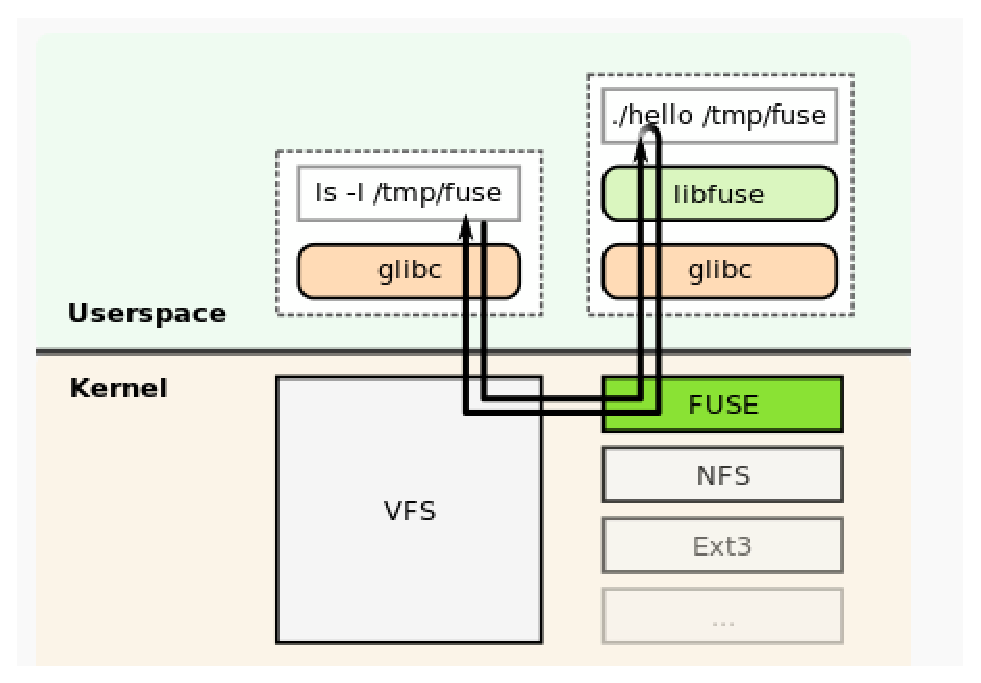
\includegraphics[height=6cm,
    angle=0]{./images/FUSE.eps}}
\caption{FUSE: flow-chart diagram}
\label{fig:FUSE}
\end{figure}

\subsection{VFS}

To support different file systems, Linux has a {\bf Virtual File System} (VFS)
layer. VFS describes the system's files in terms of {\bf superblocks} and inodes
in much the same way as the EXT2 file system uses superblocks and inodes
(Sect.\ref{sec:EXT2}).
As each file system is initialised, it registers itself with the VFS. The real
file systems are either built into the kernel itself or are built as loadable
modules. 

When a block device based file system is mounted, and this includes the root
file system, the VFS must read its superblock. The VFS keeps a list of the
mounted file systems in the system together with their VFS superblocks. Each VFS
superblock contains information and pointers to routines that perform particular
functions. 

Each VFS superblock contains a pointer to the first VFS inode on the file
system. For the root file system, this is the inode that represents the ``/''
directory. The VFS also keeps a cache of directory lookups so that the inodes
for frequently used directories can be quickly found.
\url{http://www.tldp.org/LDP/tlk/fs/filesystem.html}

All file systems, of whatever type, are mounted onto a directory and the files
of the mounted file system cover up the existing contents of that directory.
This directory is known as the mount directory or mount point. When the file
system is unmounted, the mount directory's own files are once again revealed.  


\subsection{FUSE}

One of the more recent directions in file system is to enable Filesystems
in User Space. It means that user can add support to new file system without
recompiling the O/S kernel. 

\chapter{Dedicated data server}

Typically, you can have one data server or multiple data servers.


Servers assigned roles: metadata, data, or both


\section{metadata server}
\label{sec:metadata-server}

Metadata server (MDS) stores directory and file metadata
(Sect.\ref{sec:metadata-in-a-block-oriented-filesystem}).
Often a single metadata server stores all metadata for file system.

\chapter{Distributed Filesystem}
\label{chap:distributed_filesystem}

A brief information is given in Sect.\ref{sec:distributed_filesystem}. Most of
the open-source distributed filesystem have been implemented for Linux.
In Hadoop, the default file system is HDFS; yet we can also use other options
\begin{itemize}
  \item open-source: GlusterFS, Quantcast File System
  \item commercial options: Isilon OneFS, Netapp
  \item cloud-based storage system: S3 (Amazon's Simple Storage System)
\end{itemize}

\section{Google FS (Colossus)}
\label{sec:GoogleFS}


The new version of Google FS is named Colossus. 


\section{Hadoop FS (HDFS)}
\label{sec:HadoopFS} 

HDFS is a highly fault-tolerant distributed file system, developed as
part of Hadoop (Sect.\ref{chap:Hadoop}).

Like Hadoop in general, HDFS is designed to be deployed on low-cost hardware.
While most block-structured file systems use a block size on the order of 4 or 8
KB; Hadoop splits files into large blocks (default 64MB or 128MB) and distribute
the blocks among the nodes in the cluster. This allows HDFS to decrease the
amount of metadata storage required per file (the list of blocks per file will
be smaller as the size of individual blocks increases).  A wrapper to HDFS is
HBase (Chapter \ref{chap:HBase}).

Because of the relatively low amount of metadata per file (it only tracks file
names, permissions, and the locations of each block of each file), all of this
information can be stored in the main memory of the NameNode machine, allowing
fast access to the metadata.

HDFS allows for fast streaming reads of data, by keeping large amounts of data
sequentially laid out on the disk. The consequence of this decision is that HDFS
expects to have very large files, and expects them to be read sequentially.
Thus, EXT4 filesystem is considered a good option.

You cannot interact with HDFS-stored files using ordinary Linux file
modification tools (e.g., ls, cp, mv, etc). Because HDFS stores files as a set
of large blocks across several machines, these files are not part of the
ordinary file system. HDFS runs in a separate namespace, isolated from the
contents of your local files.
The files inside HDFS (or more accurately: the blocks that make them up) are
stored in a particular directory managed by the DataNode service, but the files
will named only with block ids.

HDFS does come with its own utilities for file management, which act very
similar to these familiar tools.
To open a file, a client contacts the NameNode and retrieves a list of locations
for the blocks that comprise the file.
Clients then read file data directly from the DataNode servers, possibly in
parallel. The NameNode is not directly involved in this bulk data transfer,
keeping its overhead to a minimum. 

Just as with a standard file system, Hadoop allows for storage of data in any
format, whether it's text, binary, images, etc. Hadoop also provides built-in
support for a number of formats optimized for Hadoop storage and processing,
text files, {\bf SequenceFile}, or more complex (but also more functionally
rich) options like Avro and Parquet. It's possible to create your own custom
file format in Hadoop as well.

There are several Hadoop specific file formats that were specifically created to
work well with MapReduce. These Hadoop specific file formats include file based
data structures such as sequence files, serialization formats like Avro, and
columnar formats such as RCFiles and Parquet.   These file formats have
differing strengths and weaknesses, but all share the following characteristics
that are important for Hadoop applications: 
\begin{itemize}
  \item splittable compression
  \item agnostic compression: the file can be compressed with any compression
  method, without readers having to know the codec.
\end{itemize}
The SequenceFile format is one of most commonly used file based format in
Hadoop, but other file based formats are available such as MapFiles, SetFiles,
ArrayFiles, and BloomMapFiles. Since these formats were specifically designed to
work with MapReduce, they offer a high level of integration for all forms of
MapReduce jobs, including those run via Pig and Hive.    
\url{https://www.safaribooksonline.com/library/view/hadoop-application-architectures/9781491910313/ch01.html}

The first step is to copy data onto the HDFS, i.e. the {\bf ingestion process}.
The following list describes which tools to use for data from a particular
source or data format
\begin{itemize}
  \item \ldots : Talend
  \url{http://en.wikipedia.org/wiki/Talend}
  
  
  \item RDBMS: use Apache Sqoop or HBase, or MapR M7 tables
  
  Example: 1 TB of data take 3hr of ingestion using Sqoop.
  
  HBase and M7 have identical API and differ only in what kind of latencies you
  can expect
  
  \item Bulk file: use FTP and then ETL tools to load into HDFS
  
  ETL tool are too generic for the actual cases at hand. Usually, the ETL tools
  provide a way of running custom code as part of the work flow, which is a
  solution. 
  
  \item Realtime Data: using WebService + Flume (log aggregation, near
  real-time loading - near real-time means latency about less than half a day)
  \item Realtime data: (continuous stream ingestion) Storm.
  
   Flume is good at transport and some light enrichment / decoration. Storm can
  actually do real-time heavy lifting.
  
  \item (not using HDFS, but use NFS): Customers of MapR's Hadoop distribution
  typically utilize NFS to ingest data (and subsequently make it available to
  other parts of the organization, either in a Hadoop context or not). They
  often find NFS easier to use than Flume, legacy ETL/ELT processes and the
  like. (Note that I work for MapR).
\end{itemize}
The choice depending on the data source at latency requirements.
\url{https://www.linkedin.com/groups/Data-Ingestion-Into-Hadoop-3638279.S.199779955}

Data stored in HDFS are just bytes, i.e. there is no datatypes. 
To access these data, there are several options:
\begin{enumerate}
  \item MapReduce jobs: write your own Java/C/C++ code in MapReduce jobs
  (Chap.\ref{chap:Hadoop})
  
  \item HBase's API (in Java, REST, Thrift): (Chap.\ref{chap:HBase})
  \item Move data from HDFS to relational database systems: To move data between
  HDFS and relational database, we can use Apache Sqoop.
\end{enumerate}
 


\subsection{text files (CSV, XML)}

A very common use of Hadoop is the storage and analysis of logs such as web logs
and server logs. Such text data, of course, also come in many other forms: CSV
files, or unstructured data such as emails, etc 

The data stored in HDFS can be either {\it text files} or {\it sequence files}
in the form of (key,value) pairs. Sequence files are appropriate for situations
where you want to store the keys and their corresponding values. In text files,
we can do that but we have to parse each line. The sequence file can be
compressed and still be splittable, i.e. better workload. We cannot split a
compressed text file, unless we use a splittable compresion format. Thirdly, a
sequence file can be approached as a binary files, i.e. more storage efficient;
while in text files, double values will be stored as a number of characters,
i.e. large storage overhead.

For example, when storing 1234 in a text file and using it as an integer,
requires a String to Integer conversion during read, and vice-versa during
writing. This overhead adds up when you do a lot of such conversions. 

A more specialized form of text files are structured formats such as XML and
JSON. These types of formats can present special challenges with Hadoop since
splitting XML and JSON files for processing is tricky, and Hadoop does not
provide a built-in InputFormat for either of these formats. JSON presents even
greater challenges than XML, since there are no tokens to mark the beginning or
end of a record. In the case of these formats, you have a couple of options:     
\begin{itemize}
  \item Avro: as a container format, Transforming the data into Avro can provide
  a compact and efficient way to store and process the data.
  
  \item Pig: use a library designed for processing XML or JSON files, e.g.
  XMLLoader in PiggyBank library; or with JSON using LzoJsonInputFormat in
  Elephant Bird project. 
  
\end{itemize}

\subsection{Binary format}

For most cases of storing and processing binary files in Hadoop, and the file
size is small, using a container format such as SequenceFile is preferred
(Sect.\ref{sec:SequenceFile}). If the splittable unit of binary data is larger
than 64 MB, you may consider putting the data in it's own file, without using a
container format.


\subsection{SequenceFile}
\label{sec:SequenceFile}


HDFS works well with large files, as every 'map' task processes a block of data
at a time, which is only efficient if the block of data is large enough.
To solve the problem of storing small files in HDFS, {\bf SequenceFile} are
used as a container to store small files. It is a flat file consisting of binary
key/value pairs. Internally, the temporary output of ``map'' operator are also
in SequenceFile. 

Hadoop's SequenceFile is a persistent data structure for binary key-value pairs.
Unlike other B-tree structure, we cannot do key editting, adding or removing it.
It means that the file is append-only. 

There are 3 different SequenceFile formats
\begin{itemize}
  \item uncompressed key/value records
  \item record compressed key/value record - only 'value' are compressed here
  \item block compressed keyvalue record - both 'key' and 'value' are collected
  in 'blocks' separately and compressed. The size of 'block' is configurable. 
\end{itemize}
\url{http://wiki.apache.org/hadoop/SequenceFile}


So, user may need to write a custom reader to interpret the data to tell Hadoop
which one is key, which one is value. 

\subsection{Serialization formats (Writables, Avro, Protocol Buffers, Thrift)}
\label{sec:Serialization_hadoop}

Serialization (Sect.\ref{sec:serialization}) is core to a distributed processing
system such as Hadoop, since it allows data to be converted into a format that
can be efficiently stored as well as transferred across a network connection. 
The main serialization format utilized by Hadoop is Writables. There are,
however, other serialization frameworks seeing increased use within the Hadoop
ecosystem, including Thrift, Protocol Buffers, and Avro.  Of these, Avro is the
best suited, since it was specifically created to address limitations of Hadoop
Writables.

While Avro defines a small number of primitive types such as boolean, int,
float, and string, it also supports supports complex types such as array, map, and enum.

\subsection{columnar formats (RCFile, ORC, Parquet)}

More recently, a number of databases have introduced columnar storage, which
provides several benefits over earlier row-oriented systems. Not surprisingly,
columnar file formats are also being utilized for Hadoop applications. Columnar
file formats supported on Hadoop include the RCFile format  which has been
popular for some time as a Hive format, as well as newer formats such as ORC and
Parquet which are described below. 



\section{GSS}
\label{sec:GSS}


\section{IBM GPFS}

GPFS is built on the solid foundation of GSS (Sect.\ref{sec:GSS})

It can be deployed in shared-disk or shared-nothing distributed parallel modes.
It is used by many of the world's largest commercial companies, as well as some
of the supercomputers on the Top 500 List. GPFS provides concurrent high-speed
file access to applications executing on multiple nodes of clusters.

To achieve high throughput to a single large file, data
must be striped across multiple disks.

\subsection{GPFS 3.1}

Starting with GPFS 3.1, the structural limit on the maximum number of disks in
a file system increased from 2048 to 4096 (each 1TB); however, IBM Spectrum
Scale still enforces the original limit of 2048 

\section{GPFS Native RAID (declustered RAID): software implementation
micro-RAID}

With micro-RAID,  RAID is done at a block level as opposed to a disk level. 
This generally means that the cost of rebuilds can be reduced and the time to
get back to a protected level can be shortened. 

NOTE: As disks continue to get larger, conventional RAID implementations
struggle and you can be looking at hours if not days to get back to a protected
state.







\section{OpenAFS}
\label{sec:OpenAFS}

\url{http://www.openafs.org/}

\section{Data ingestion}
\label{sec:data_ingestion}

Data ingestion depends on
\begin{itemize}
  \item CPU 
  \item RAM
  \item Network card
  \item Harddrive
  \item Network bandwidth
\end{itemize}
\url{http://www.slideshare.net/Hadoop_Summit/mc-cuch-zhurakouskyjune261210pmroom212}

\section{GlusterFS}

GlusterFS can also be used in Hadoop, in place of HDFS.

\section{Quantcast File System}

Quantcase File System can also be used in Hadoop, in place of HDFS.

\part{Inter-process communication}
\import*{../C-Cpp_Manual/}{Socket.tex}
\import*{../Python_Manual/}{ObjectSerialization.tex}
\import*{../Sys_admin/}{OS_kernels.tex}
\import*{../Linux_Computing/}{InterProcessCommunication.tex}

\part{Distributed Computing Platform}
\chapter{Hadoop}
\label{chap:Hadoop}

Hadoop started in 2006 based on Google's work of GFS (now is called HDFS -
Sect.\ref{sec:HadoopFS}) and MapReduce. Nowadays, Hadoop 2.x is much bigger with
many more components (Sect.\ref{sec:MR1_MR2}).

\section{Why Hadoop was developed?}

Big data is not just big in terms of bytes, but also type (e.g., a single hard
disk likely contains relations, text, images, and spreadsheets) and structure
(e.g., a large corpus of relational databases may have millions of unique
schemas). As a result, certain long-held assumptions --- e.g., that the database
schema is always known before writing a query --- are no longer useful guides
for building data management systems.

Hadoop has emerged from a solution for large-scale web-crawling and indexing
engine to a general-purpose computing platform for the next-generation of
data-based applications. 

Hadoop uses two-step disk-based MapReduce implementation on Hadoop HDFS. To
enable using data on HDFS for other tasks, e.g. machine learning where iterative
algorithms are often used, there are several packages have been developed:
Apache Spark (Sect.\ref{sec:apache_spark}).

\subsection{Hadoop is NOT}

\begin{itemize}
  \item ESB
  \item NoSQL
  \item HPC
  \item Relational 
  \item Real-time
\end{itemize}

Data is added into the HDFS system, but you cannot ask Hadoop to return a list
of all the data matching a specific data set. 
The primary reason for this is that Hadoop doesn't store, structure, or
understand the structure of the data that is being stored within HDFS. One
soltuion is to use HBase (a distributed database system on top of HDFS). 

\subsection{Key Hadoop data types}

The below types of data are widely added to HDFS (Sect.\ref{sec:HadoopFS})
\begin{itemize}
  \item Sentiment
  \item Clickstream
  \item Sensor/Machine
  \item Geographic
  \item Server logs
  \item Text
\end{itemize}


\section{Critics of Hadoop}

It was designed to run on-premises in data centers with the advantage of using
low-cost machines.
But now everyone is moving to cloud. Y

\begin{enumerate}
  \item ou can run Hadoop in the cloud. But it is not cost effective.

  \item  Hadoop is getting fatter with so different components.
  
  Today, the architecture picture
  of Hadoop looks like a zoo hosting HDFS, YARN, MapReduce, Tez, Pig, Hive,
  Impala, Kudu, HBase, Accumulo, Flume, Sqoop, Falcon, Samza, etc.
  
  Because original Hadoop (with only HDFS and MapReduce) is not good enough to
  meet customer's demands, the community has developed a lot of new tools into
  the Hadoop ecosystem over the years.
  
  This is rational and necessary to win the competition. However, it also
  inevitably reaches the status of overshooting. 
  
  
 Rarely customers need all of them. If no need, why bother running a full blown
 Hadoop cluster? So, options to pick only needed components such as
 \begin{itemize}
   \item  Parquet + Spark
   
   \item Apache Samza, a stream processing engine that was originally designed
   on top of Hadoop YARN
   
   Netflix has recently contributed the feature of static partition assignments
   that allows Samza to be used without YARN. This cool feature enables Netflix
   to run Samza applications in AWS EC2 instances without any Hadoop/YARN
   dependency.
 \end{itemize}
  
  \item HBase, the NoSQL engine of Hadoop, is not as competitive as other noSQL
  solutions.
  
  Compared to other popular NoSQL solutions such as MongoDB and Cassandra, HBase
  has a lot of functionality and unique features. It also has battle proven
  scalability and availability.
  Moreover, Apache Trafodion, built on top of HBase, even provides fully ACID
  SQL. However, it is only ranked at 15 on DB-Engines Ranking, way behind
  MongoDB and Cassandra. The biggest reason that HBase is left behind is that
  Hadoop distributors' marketing commitment to HBase has never risen to nearly
  the level of MongoDB's or DataStax's push behind their respective core
  products.
  
  Technically, HBase is also more complicated to setup and operate because of
  the dependency to other Hadoop services.
  
  \item Spark, Kafka, Mesos, Docker, etc. are better than their counterparts of
  Hadoop or fill in blank space. And they get endorsements from heavy weights
  like IBM. 
\end{enumerate}
\url{https://haifengl.wordpress.com/2016/03/03/the-future-of-hadoop-is-misty/}


\section{Hadoop distributors}

Apache Hadoop is the main open-source repository for Hadoop development. Other
than that, there are 3 main Hadoop distributions, target to commercial licenses
\begin{enumerate}
  \item Cloudera CDH: plan to provide ``enterprise datahub'', i.e. there is no
  need for datawarehouse at company
  
  It has free version and commercial version. Some features are not open-source.
  
  \item Hortonwork Hadoop: this is the 100\% open-source distribution, and the
  main driver for Hadoop development at Apache, e.g. YARN module.
  
  \item MapR Hadoop: this one does not use HDFS, but use MapRFS (a proprietary
  distributed file system). 
  
  The free version is MapR's M3 Edition. It provides proprietary modules to ease
  the maintenance and usage of a Hadoop system at companies which do not have
  programmers/experts in Hadoop.
\end{enumerate}
All of these products are rooted from Apache Hadoop.

\section{Apache Hadoop}

A Hadoop cluster is a special type of computational cluster designed
specifically for storing and analyzing huge amounts of unstructured data in a
distributed computing environment. As of early 2013, Facebook was recognized as
having the largest Hadoop cluster in the world. Other prominent users include
Google, Yahoo and IBM. These clusters use Hadoop framework. 

Hadoop has its origin from Apache Nutch (Sect.\ref{sec:Nutch}).
The 2 components in Nutch were applicable beyond the realm of search, and thus
an independent project was created in Feb, 2006 called Hadoop. Then Doug Cutting
joined Yahoo, and help to turn Hadoop into a system that ran at web scale, e.g.
10,000-core Hadoop cluster. In Jan, 2008, Apache Hadoop become the top-level
project. 

In April 2008, Hadoop broke a world record to become the fastest system to sort
a terabyte of data. Running on a 910-node cluster, Hadoop sorted one terabyte in
209 seconds (just under $3^\frac{1}{2}$ minutes), beating the previous year's winner
of 297 seconds. In November of the same year, Google reported that its MapReduce
implementation sorted one terabyte in 68 seconds. Then a team at
Yahoo! used Hadoop to sort one terabyte in 62 seconds.

Hadoop framework is written in Java that enables running a Java app on large
clusters of commodity hardware (i.e. low costs) as it's running on a single
machine. Hadoop's HDFS is the distributed file system (Sect.\ref{sec:HadoopFS}).
It should be installed in a cluster. However, we can deploy on a single machine
by configuring a pseudo-distributed single-node Hadoop cluster.

The project's creator, Doug Cutting, explains how the name came about:
\begin{verbatim}
The name my kid gave a stuffed yellow elephant. Short, relatively easy to spell
and pronounce, meaningless, and not used elsewhere: those are my naming
criteria. Kids are good at generating such. Googol is a kid's term.  
\end{verbatim} 
Subprojects and ``contrib" modules in Hadoop also tend to have names that are
unrelated to their function, often with an elephant or other animal theme
(``Pig," for example). Smaller components are given more descriptive (and
therefore more mundane) names. This is a good principle, as it means you can
generally work out what something does from its name. For example, the
jobtracker keeps track of MapReduce jobs.    

Hadoop Ecosystem, which includes all of the additional software packages that
can be installed on top of or alongside Hadoop, such as Apache Hive, Apache Pig
and Apache Spark. Hadoop is Consistent and partition tolerant, i.e. it falls
under the CP category of the CAP theoram.
\begin{enumerate}
  \item Hadoop Common
  \item Hadoop HDFS:
  \item Hadoop YARN (added from Hadoop 2.0):  resource-management platform
  responsible for managing compute resources in clusters and using them for scheduling of users' applications.
  \item Hadoop MapReduce: a programming model for large scale data processing.
\end{enumerate}

\subsection{Hadoop computing engine}
\label{sec:hadoop_node_structure}

For processing the data, the Hadoop Map/Reduce ships code (typically Java-code
.jar file) to to the nodes that have the required data, and the nodes then
process the data in parallel. So, each node functions as ``data'' source and
computing unit which takes advantage of data locality. \textcolor{red}{This is
in contrast to HPC architecture which split data cluster and compute cluster,
but connect through high-speed networking}. 

Although Java code is common, any programming language can be used with "Hadoop
Streaming" to implement the "map" and "reduce" parts of the user's program. To
expose higher level APIs, Apache Pig, Apache Hive and Apache Spark have been
added. 
\url{http://en.wikipedia.org/wiki/Apache_Hadoop}

Next, you need to know the structure of a Hadoop cluster. 
A small Hadoop cluster includes a single master (which functions as both
NameNode and JobTracker) and multiple worker nodes.
The master node can function as a JobTracker (Resource Manager), TaskTracker
(NodeManager), NameNode and DataNode.
A slave or worker node acts as both a DataNode and TaskTracker, though it is
possible to have data-only worker nodes and compute-only worker nodes. NOTE:
TaskTracker are compute-node.

\begin{enumerate}
  \item one machine as NameNode, one machine as Resource Manager (or aka
  JobTracker).
    
  These machines are the masters.
  \begin{itemize}
    \item NameNode stores HDFS filesystem information in a file named
    \verb!fsimage!. Updates to the file system (add/remove blocks) are not
    updating the fsimage file, but instead are logged into a file, so the I/O
    is fast append only streaming as opposed to random file writes. Only when
    restaring, before it can serve client requests, the namenode reads the
    fsimage and then applies all the changes from the log file to bring the filesystem state up to date in
    memory (a new fsimage consisting of the prior fsimage plus the application
    of all operations from the edit logs). It remains in safe mode until a
    sufficient number of blocks have been reported by datanodes. This process
    takes time. Administrators typically access the NameNode web UI at the first
    sign of trouble.  Unfortunately, the NameNode wouldn't start its HTTP server
    until after writing a new checkpoint.  In a slow startup situation, it could
    take multiple minutes or even more than an hour after restarting the
    NameNode before the web UI would be accessible which makes it would appear
    as though the NameNode process had hung during startup.
    Only an experienced Hadoop operator would be able to determine that the
    NameNode is in fact making progress, by using relatively low-level
    techniques such as inspecting thread dumps.
    \footnote{\url{http://hortonworks.com/blog/understanding-namenode-startup-operations-in-hdfs/}}
    
    Since Hadoop 2.0, a new feature called Secondary NameNode added. What it
    does is to help boosting the start-up time; not as a full replicate of the
    NamaNode.\footnote{\url{http://stackoverflow.com/questions/19970461/name-node-vs-secondary-name-node}}
    
    
  \end{itemize}
  
  \item The rest of the machines: act as both DataNode and NodeManager
  (TaskTracker).
  
  All these machines depend on the NameNode. If the name node falls the cluster
  goes down.
  
  \item (optional) one machine as Secondary NameNode: this machine does not
  function as a seconday to the NameNode machine. Instead,  it periodically read
  the filesystem changes log and apply them into the fsimage file, thus bringing
  the fsimage file up to date so that the NameNode start up faster next time.
  No slaves can connect to the Secondary NameNode; so if the NameNode is down,
  the whole Hadoop cluster still fails.
  
\end{enumerate}
In a larger cluster, the HDFS is managed through a dedicated NameNode server to
host the file system index, and a Secondary NameNode that can generate snapshots
of the namenode's memory structures, thus preventing file-system corruption and
reducing loss of data. Similarly, a standalone JobTracker server (Resource
Manager) can manage job scheduling.


Your MapReduce jobs may be IO bound or CPU/Memory bound -if you know which one
is more important (effectively how many CPU cycles/RAM MB used per Map or
Reduce), you can make better decisions. 


\subsection{Hadoop YARN}
\label{sec:YARN}

Yarn has been added to Hadoop 2.0. 
With YARN, you can now run multiple applications in Hadoop, all sharing a common
resource management.  As of September, 2014, YARN manages only CPU (number of
cores) and memory, but management of other resources such as disk, network
and GPU is planned for the future.



\subsection{User authentication and authorization}

Hadoop doesn't do any authentication of users. This is an important realization
to make, because it can have serious implications in a corporate data center.
The NameNode and the JobTracker don't require any authentication.
Hadoop has the ability to require authentication, in the form of Kerberos
principals (Sect.\ref{sec:Kerberos}). 

Hadoop can use the Kerberos protocol to ensure that when someone
makes a request, they really are who they say they are. This mechanism is used
throughout the cluster. In a secure Hadoop configuration, all of the Hadoop
daemons use Kerberos to perform mutual authentication, which means that when two
daemons talk to each other, they each make sure that the other daemon is who it
says it is. Additionally, this allows the NameNode and JobTracker to ensure that
any HDFS or MR requests are being executed with the appropriate authorization
level.

HDFS implement a permission model much like POSIX model. Each file and directory
is associated with an owner and a group. The file or directory has separate
permissions for the user that is the owner, for other users that are members of
the group, and for all other users.  The difference from POSIX:
\begin{verbatim}
In contrast to the POSIX model, there are no setuid or setgid bits for files as
there is no notion of executable files.

For directories, there are no setuid or setgid bits directory as a
simplification..

The Sticky bit can be set on directories, preventing anyone except the
superuser, directory owner or file owner from deleting or moving the files
within the directory. Setting the sticky bit for a file has no effect.
\end{verbatim}

In the context of MapReduce, the users and groups are used to determine who is
allowed to submit or modify jobs. In MapReduce, jobs are submitted via queues
controlled by the scheduler.
Administrators can define who is allowed to submit jobs to particular queues via
MapReduce ACLs (Access Control Lists).  


The downside to doing this is that if that user and group really don't exist, no
one will be able to access that file except the superusers, which, by default,
includes hdfs, mapred, and other members of the hadoop supergroup.  


% \section{Experiences with Hadoop}
% 

\subsection{Configure environment: hadoop-env.sh}
\label{sec:hadoop-env.sh}

Administrators should use the conf/hadoop-env.sh script to do site-specific
customization of the Hadoop daemons' process environment.

The file
\begin{verbatim}
/usr/local/hadoop/etc/hadoop/hadoop-env.sh
\end{verbatim}
control the path to java, and the setting for the four different
daemons NameNode/DataNode and JobTracker/TaskTracker. Each daemon receives
configuration options specified in the associated environment variable, which
maps to
\begin{verbatim}
NameNode           	HADOOP_NAMENODE_OPTS
DataNode            HADOOP_DATANODE_OPTS
SecondaryNameNode   HADOOP_SECONDARYNAMENODE_OPTS
JobTracker          HADOOP_JOBTRACKER_OPTS
TaskTracker         HADOOP_TASKTRACKER_OPTS
\end{verbatim}
%different locations which contaisn files that Hadoop needs to use, and the
% different system settings, e.g. maximum heap size

As Hadoop is used to run Java applications (hadoop daemons), these settings are
designed to control how a Java MapReduce applications run and use resources
\begin{verbatim}
JAVA_HOME
HADOOP_OPTS (extra args to java-runtime, default:  
            -Djava.net.preferIPv4Stack=true)

HADOOP_CONF_DIR

JSVC_HOME

HADOOP_CLASSPATH

# max heap to use
HADOOP_HEAPSIZE (in MB, default:1000)
HADOOP_NAMENODE_INIT_HEAPSIZE (in MB, default: 1000)

## 
HADOOP_NAMENODE_OPTS
  "-Dhadoop.security.logger=${HADOOP_SECURITY_LOGGER:-INFO,RFAS}
  -Dhdfs.audit.logger=${HDFS_AUDIT_LOGGER:-INFO,NullAppender} $HADOOP_NAMENODE_OPTS"
HADOOP_DATANODE_OPTS
  "-Dhadoop.security.logger=ERROR,RFAS $HADOOP_DATANODE_OPTS"
HADOOP_SECONDARYNAMENODE_OPTS

HADOOP_NFS3_OPTS
HADOOP_PORTMAP_OPTS (default: -Xmx512m)

## apply to commands such as: fs, dfs, fschk, distcp
HADOOP_CLIENTS_OPTS (default: -Xmx512m)
HADOOP_JAVA_PLATFORM_OPTS


# secure DataNode
HADOOP_SECURE_DN_USER

# location of log file
HADOOP_LOG_DIR (default: $HADOOP_HOME/logs)
          (we can use $HADOOP_LOG_DIR/$USER)
HADOOP_SECURE_DN_LOG_DIR (default: ${HADOOP_LOG_DIR}/${HADOOP_HDFS_USER})


# location of PID file
HADOOP_PID_DIR    (default: /tmp)
        however should be set to a location that is accessible by only the 
        'hadoop' group's users, to avoid potential symlink attack
HADOOP_SECURE_DN_PID_DIR

# a string representation of the instance of hadoop
HADOOP_IDENT_STRING   (default: $USER) 

\end{verbatim}

Example: enable parallelGC  on NameNode daemon
\begin{verbatim}
export HADOOP_NAMENODE_OPTS="-XX:+UseParallelGC ${HADOOP_NAMENODE_OPTS}" 
\end{verbatim}

Example: in a multi-user Hadoop cluster, you may need to configure the log dir
\begin{verbatim}
HADOOP_LOG_DIR
\end{verbatim}

Example: maximum heapsize (in MB) for each daemon (default: 1000MB)
\begin{verbatim}
HADOOP_HEAPSIZE
\end{verbatim}

\section{Changes from Hadoop 1.x to Hadoop 2.x}
\label{sec:MR1_MR2}

Hadoop 1.x basically has 2 components: HDFS and MapReduce.

Hadoop 2.x has revised and break MapReduce down into different projects, each
does a particular job. A new and important layer above HDFS is YARN (batch
processing management) which allows new components to be added (Spark, BSP,
Hama, MapReduce, HBase (database system)) or existing programming models to use
(e.g. MPI). \url{http://www.wiziq.com/blog/hadoop-1-vs-hadoop-2/}

\subsection{Hadoop 1}

\begin{enumerate}
  \item Limited up to 4000-nodes per cluster
  \item The bottleneck is based on the number of tasks in a cluster: O(\# tasks
  in a cluster)
  
  \item JobTracker does multiple things: resource management, job scheduling and
  monitoring $\rightarrow$ which causes the bottleneck
  
  \item Only one namespace for managing HDFS
  \item Map and Reduce slots are static
  \item only job to run is MapReduce.
  
  \item The namespaces for APIs
\begin{verbatim}
org.apache.hadoop.mapreduce.Partitioner
org.apache.hadoop.mapreduce.Mapper
org.apache.hadoop.mapreduce.Reducer
org.apache.hadoop.mapreduce.Job
\end{verbatim} 
\end{enumerate}


\url{http://www.slideshare.net/RommelGarcia2/hadoop-1x-vs-2}

\begin{figure}[hbt]
  \centerline{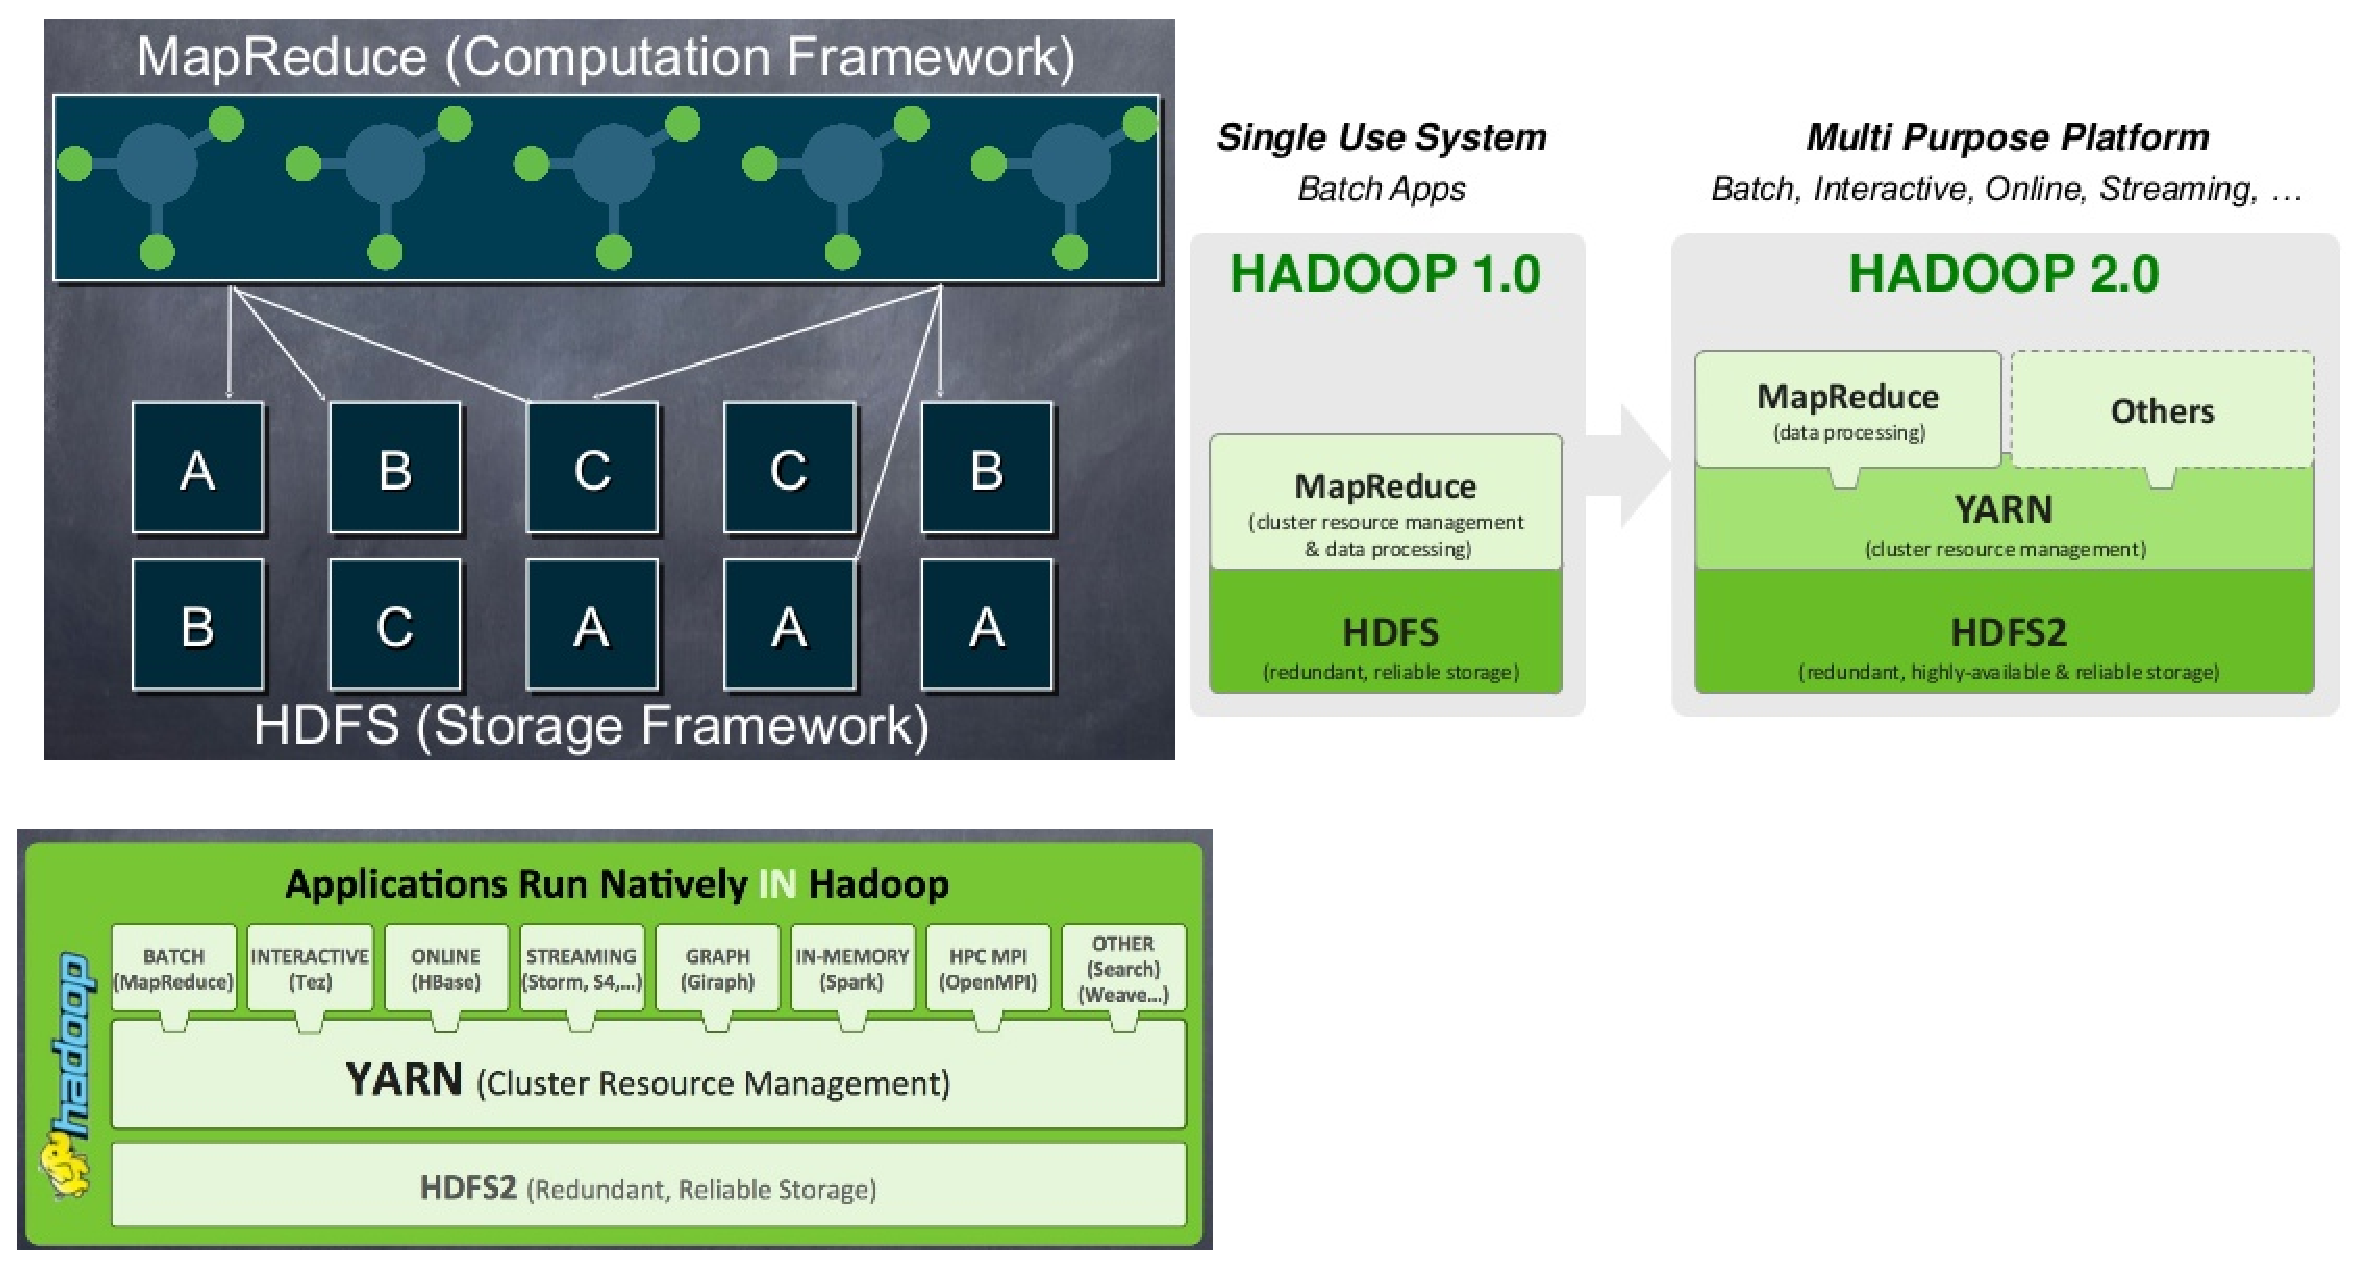
\includegraphics[height=6cm,
    angle=0]{./images/MR1_MR2_comparison_01.eps}}
  \caption{MR1 to MR2}
  \label{fig:MR1_MR2_comparison_01}
\end{figure}


\subsection{Hadoop 2}

backward compatible with MR1
\begin{enumerate}
  \item Support upto to 10,000 nodes per cluster
  \item The bottleneck is based on the cluster size: O(cluster size)
  \item The function of JobTracker in MR1 is different in MR2. To avoid
  scaling issues, JobTracker is splitted into different components, each with
  its specialized purpose (see below). Resource manager is carried out by the new component: YARN.
  
  \item multiple namespace for managing HDFS, Fig.\ref{fig:MR1_MR2_comparison_02}
  \item YARN is used as Resource Manager.
\begin{verbatim}
org.apache.hadoop.yarn.api.ApplicationClientProtocol
org.apache.hadoop.yarn.api.ApplicationMasterProtocol
org.apache.hadoop.yarn.api.ContainerManagementProtocol
\end{verbatim}  
  
  \item HDFS support multiple storage tiers: Disk, Memory, SSD
  
  \item any job can be integrated with Hadoop
  \item support other languages (not only Java)
\end{enumerate}
\url{http://www.slideshare.net/tshooter/strata-conf2014}

\begin{figure}[hbt]
  \centerline{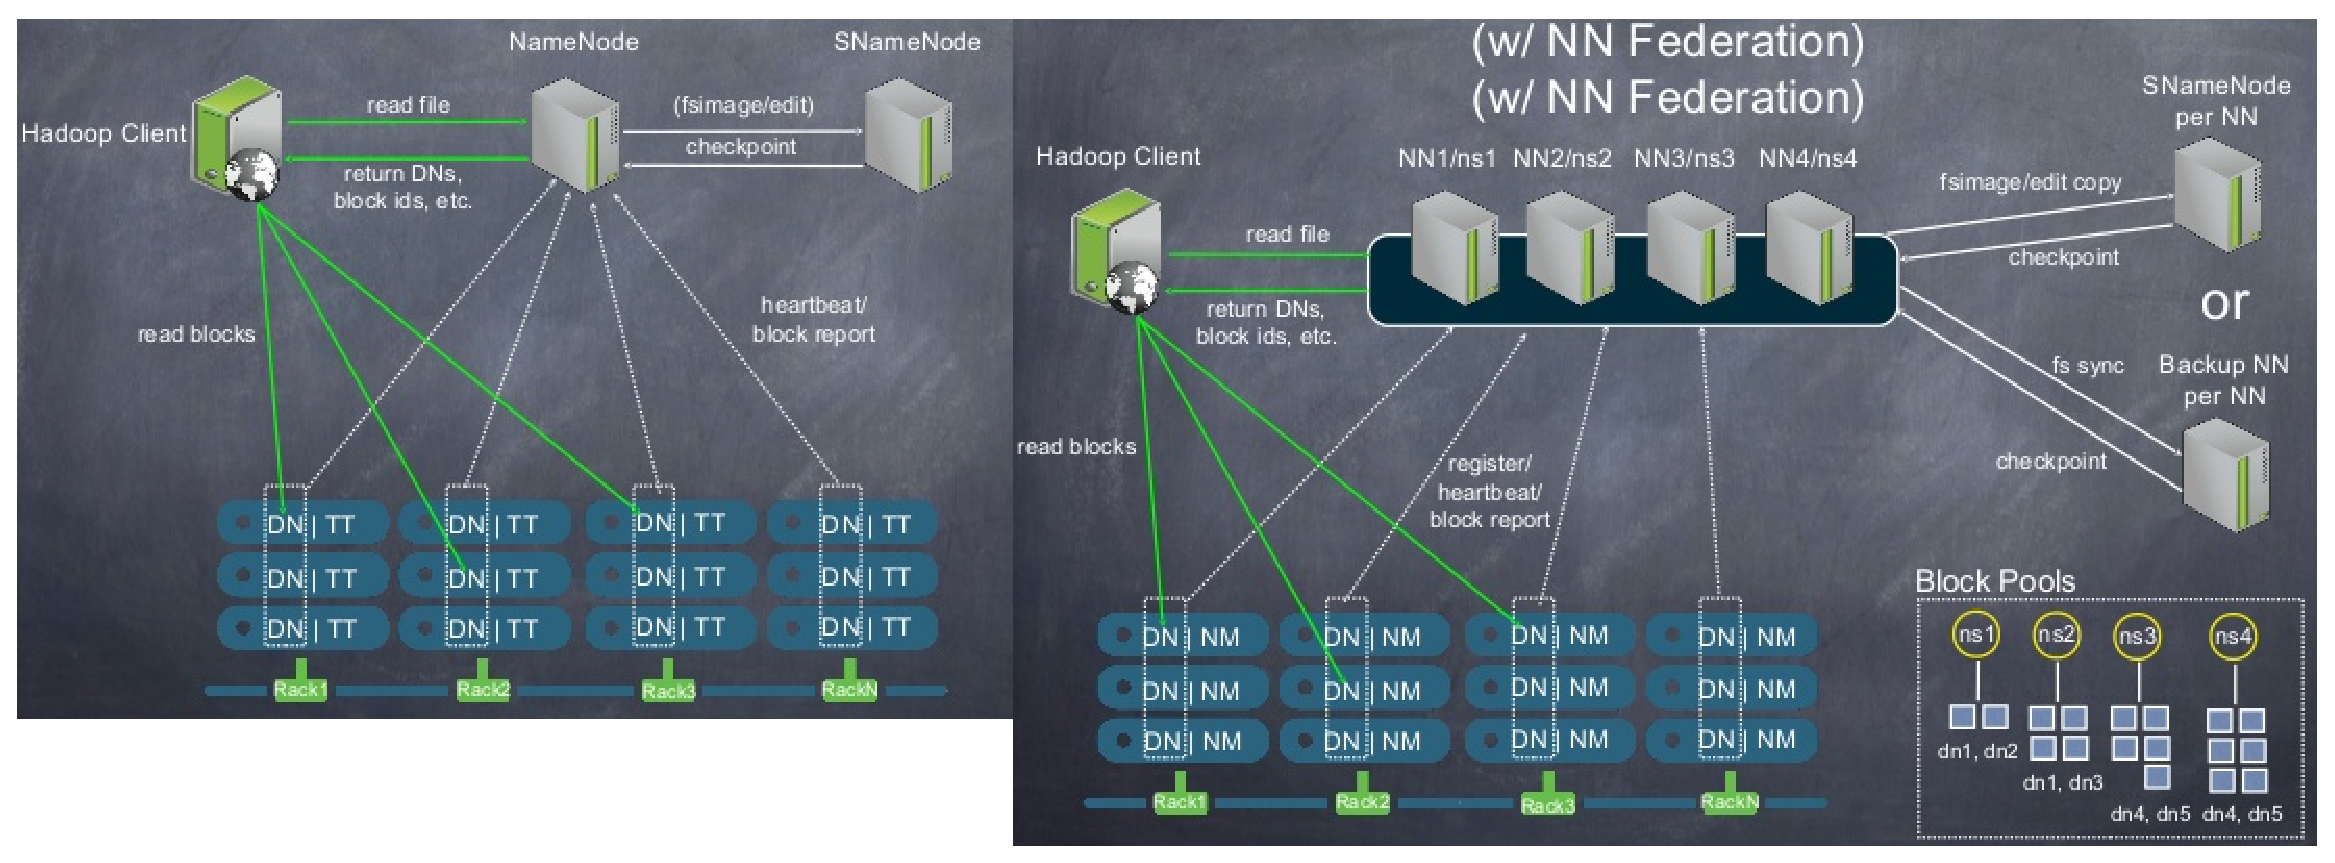
\includegraphics[height=3cm,
    angle=0]{./images/MR1_MR2_comparison_02.eps}}
  \caption{MR1 to MR2 comparison: Data can reside on NameNodes of different
  namespace}
  \label{fig:MR1_MR2_comparison_02}
\end{figure}

The reason is that in Hadoop 2, MapReduce is split into 2
components: the cluster resource management capabilities have become YARN; and
the MapReduce-specific capabilities remain MapReduce. This is known as MR2
architecture; while the old one is called MR1.
\begin{enumerate}
  \item In the former MR1 architecture, the cluster was managed by a service
  called the JobTracker.
  
  \item In MR2 architecture: the functions of the JobTracker are divided into
  three services.
  \begin{itemize}
    \item The ResourceManager is a persistent YARN service that receives and
    runs applications (a MapReduce job is an application) on the cluster
    \item 
  \end{itemize}
\end{enumerate}

\subsection{List of deprecated keys}

\url{https://hadoop.apache.org/docs/r2.2.0/hadoop-project-dist/hadoop-common/DeprecatedProperties.html}

{\small
\begin{verbatim}
[INFO] deprecation - mapred.jar is deprecated. Instead, use mapreduce.job.jar
[INFO] deprecation - mapred.map.child.log.level is deprecated. Instead, use mapreduce.map.log.level
[INFO] deprecation - mapred.reduce.child.log.level is deprecated. Instead, use mapreduce.reduce.log.level
[INFO] deprecation - mapred.output.value.groupfn.class is deprecated. Instead, use mapreduce.job.output.group.comparator.class
[INFO] deprecation - mapred.output.key.comparator.class is deprecated. Instead, use mapreduce.job.output.key.comparator.class
[INFO] deprecation - mapred.cache.files is deprecated. Instead, use mapreduce.job.cache.files
[INFO] deprecation - mapred.mapoutput.key.class is deprecated. Instead, use mapreduce.map.output.key.class
[INFO] deprecation - mapreduce.inputformat.class is deprecated. Instead, use mapreduce.job.inputformat.class
[INFO] deprecation - mapreduce.partitioner.class is deprecated. Instead, use mapreduce.job.partitioner.class
[INFO] deprecation - mapred.job.name is deprecated. Instead, use mapreduce.job.name
[INFO] deprecation - mapred.mapoutput.value.class is deprecated. Instead, use mapreduce.map.output.value.class
[INFO] deprecation - mapred.job.tracker is deprecated. Instead, use mapreduce.jobtracker.address
[INFO] deprecation - fs.default.name is deprecated. Instead, use fs.defaultFS
[INFO] deprecation - mapred.local.dir is deprecated. Instead, use mapreduce.cluster.local.dir
[INFO] deprecation - fs.checkpoint.edits.dir is deprecated. Instead, use dfs.namenode.checkpoint.edits.dir
[INFO] deprecation - dfs.data.dir is deprecated. Instead, use dfs.datanode.data.dir
[INFO] deprecation - fs.checkpoint.dir is deprecated. Instead, use dfs.namenode.checkpoint.dir
[INFO] deprecation - mapred.temp.dir is deprecated. Instead, use mapreduce.cluster.temp.dir
[INFO] deprecation - dfs.name.dir is deprecated. Instead, use dfs.namenode.name.dir
[INFO] deprecation - mapred.system.dir is deprecated. Instead, use mapreduce.jobtracker.system.dir
[INFO] deprecation - fs.default.name is deprecated. Instead, use fs.defaultFS
[INFO] deprecation - mapreduce.map.class is deprecated. Instead, use mapreduce.job.map.class
[INFO] deprecation - dfs.name.edits.dir is deprecated. Instead, use dfs.namenode.edits.dir
[INFO] deprecation - user.name is deprecated. Instead, use mapreduce.job.user.name
[INFO] deprecation - mapred.cache.files.filesizes is deprecated. Instead, use mapreduce.job.cache.files.filesizes
[INFO] deprecation - fs.default.name is deprecated. Instead, use fs.defaultFS
[INFO] deprecation - mapred.reduce.tasks is deprecated. Instead, use mapreduce.job.reduces
[INFO] deprecation - mapreduce.reduce.class is deprecated. Instead, use mapreduce.job.reduce.class
[INFO] deprecation - mapred.output.dir is deprecated. Instead, use mapreduce.output.fileoutputformat.outputdir
[INFO] deprecation - mapred.map.tasks is deprecated. Instead, use mapreduce.job.maps
[INFO] deprecation - mapred.cache.files.timestamps is deprecated. Instead, use mapreduce.job.cache.files.timestamps
[INFO] deprecation - mapred.working.dir is deprecated. Instead, use mapreduce.job.working.dir
\end{verbatim}
}
\url{https://groups.google.com/forum/#!msg/scoobi-dev/OiWMwnxpoQE/H4fjQBMF3vcJ}
\section{Resource in Hadoop}
\label{sec:Hadoop_resources}

A resource is an XML-based file that contain a set of name/value pair.

\subsection{Read-only configuration}

These files contains the read-only configuration
\begin{verbatim}
src/core/core-default.xml 
src/hdfs/hdfs-default.xml 
src/mapred/mapred-default.xml.
\end{verbatim}
It comes with some default settings. 


By default, Hadoop has 2 resources, loaded in the order they are specified
in the classpath
\begin{verbatim}
core-default.xml   # read-only information
core-site.xml      # site-specific information (for a given Hadoop installation)
\end{verbatim}

The configuration in the form
\begin{verbatim}
<property>
    <name>property-name</name>
    <value>property-value</value>

  </property>
\end{verbatim}

Example: specify 
\begin{verbatim}
<property>
  <name>dfs.datanode.data.dir</name>
  <value>file:///usr/local/hadoop/data/datanode</value>
  <description>DataNode directory</description>
</property
\end{verbatim}
we can declare a key/value pair as {\it final} (i.e. no subsequently-loaded
resource can modify the value). Typically, the {\it final} key/value pair are
stored in \verb!core-site.xml! file so that user application cannot alter.
\begin{verbatim}
<property>
    <name>dfs.client.buffer.dir</name>
    <value>/tmp/hadoop/dfs/client</value>
    <final>true</final>
  </property>
\end{verbatim}


There are so many pre-defined names from Hadoop. From your application, you can
modify these key/value pair by loading the classpath
\begin{verbatim}
java.lang.Object
    org.apache.hadoop.conf.Configuration
\end{verbatim}
with the predefined methods to handle the modification of them.
\url{http://hadoop.apache.org/docs/r1.2.1/api/org/apache/hadoop/conf/Configuration.html}

\subsection{Site-specific configuration}

These are files that contains configuration that you can modify and it is
site-specific, i.e. it can be different from one machine to another.
\begin{verbatim}
conf/core-site.xml
conf/hdfs-site.xml 
conf/mapred-site.xml
\end{verbatim}

You can control the Hadoop scripts found in the bin/ directory of the
distribution, by setting site-specific values via the conf/hadoop-env.sh
(Sect.\ref{sec:hadoop-env.sh}).

\subsection{core-site.xml}
\label{sec:core-site.xml}

The URI to the NodeName can be defined in the key \verb!fs.defaultFS! (the
deprecated key (since Hadoop 2.0) is fs.default.name)
\url{https://issues.apache.org/jira/browse/AMBARI-2789}


\subsection{yarn-site.xml}
\label{sec:yarn-site.xml}

We need to specify the machine that functions as the ResourceTracker
\begin{verbatim}
<property>
<name>yarn.resourcemanager.resource-tracker.address</name>
<value>10.10.10.104:8025</value>
</property>
<property>
\end{verbatim}

Then we choose what shuffle process to handle the 
\begin{verbatim}
<property>
   <name>yarn.nodemanager.aux-services</name>
   <value>mapreduce_shuffle</value>
</property>
<property>
   <name>yarn.nodemanager.aux-services.mapreduce_shuffle.class</name>
   <value>org.apache.hadoop.mapred.ShuffleHandler</value>
</property>
\end{verbatim}
\url{https://developer.yahoo.com/hadoop/tutorial/module1.html}

\section{Disk configuration}

\url{http://cloud-dba-journey.blogspot.com/2013/08/hadoop-reference-architectures.html}

Hadoop is quite different than other services in conventional data centers, such
as web, mail, and database servers. They are learning that to achieve optimal
performance, you need to pay particular attention to configuring the underlying
hardware.
\url{http://hortonworks.com/blog/proper-care-and-feeding-of-drives-in-a-hadoop-cluster-a-conversation-with-stackiqs-dr-bruno/}

Having lots of disks per server gives you more raw IO bandwidth than having one
or two big disks. If you have enough that different tasks can be using different
disks for input and output, disk seeking is minimized, which is one of the big
disk performance killers. That said: more disks have a higher power budget; if
you are power limited, you may want fewer but larger disks.    

\subsection{Ext3 or Ext4 or XFS or btrfs or zfs}

\textcolor{red}{Don't use LVM; it adds latency and causes a bottleneck.}  

\begin{enumerate}
  \item XFS: internally it uses B+ trees and Extends to store data. It is fully
  supported in Ubuntu. \url{https://wiki.ubuntu.com/XFS}
  \item Ext3/Ext4: use H trees
\end{enumerate}

Yahoo! has publicly stated they use ext3. Regardless of the merits of the
filesystem, that means that HDFS-on-ext3 has been publicly tested at a bigger
scale than any other underlying filesystem that we know of.


Ext4 has better performance with large files. However, the Ext4 Linux filesystem
has delayed allocation of data which makes it handle unplanned server
shutdowns/power outages less well than classic ext3. Consider turning off the
delalloc option in /etc/fstab unless you trust your UPS.

XFS offers better disk space utilization than ext3 and has much quicker disk
formatting times than ext3. This means that it is quicker to get started with a
data node using XFS. However, most often, the limitation is not disk-read, but 
I/O and RAM limitations will be more important. XFS is not included in basic
RedHat Enterprise Linux.


So, \textcolor{red}{ext3 is the most common choice.} However, since Ubuntu
12.04, the preferred one is XFS, EXT4, EXT3 in that order.

Create one single partition
\begin{verbatim}
fdisk /dev/sdb
\end{verbatim}
Format the partition with EXT4
\begin{verbatim}
mkfs.ext4 /dev/sdb1
\end{verbatim}

Automount to /data/0, /data/1 (if we have more disk)
by modifying /etc/fstab file
\begin{verbatim}	
/dev/sdb1  /data/0  ext4   defaults,noatime,nodiratime
      1    2
\end{verbatim}
NOTE: We use these as we don't need these information and thus can improve disk
performance
\begin{verbatim}
noatime = skip writing file access time to disk
          everytime a file is accessed
nodiratime = skip writing directory access time          
\end{verbatim}

\url{http://wiki.apache.org/hadoop/DiskSetup}

\url{http://hortonworks.com/kb/linux-file-systems-for-hdfs/}

\subsection{RAID or JBOD (non-RAID)}

You don't need RAID disk controllers for Hadoop Data Node, as it copies data
across multiple machines instead.
\url{http://wiki.apache.org/hadoop/DiskSetup}
A set of separate disks is better than the same set managed by
RAID-0 disk array. The reason is that read-speed can vary from disk to disk, and
in RAID-0, it runs with the speed of the slowest one. So, if you have multiple
disks, you should use comma-delimited in the configuration file to specify
multiple locations. Also, in RAID-0, a single disk failures will bring the whole
node's data down.

Without RAID, losing a single disk would cause a certain loss of data.
While drives are much more reliable than they used to be, disk failures still
can happen any time.
\begin{verbatim}
Our experience indicates that a 1,000 node cluster containing 12,000 drives for
a total raw storage capacity of 48 peta-bytes can expect about 3 drive failures
a day in its third year of operation. Drive failure rates rise as the devices
age. For a 500 node cluster, you're looking at a drive failure every 17 hours or
so. 
\end{verbatim}
\url{http://hortonworks.com/blog/proper-care-and-feeding-of-drives-in-a-hadoop-cluster-a-conversation-with-stackiqs-dr-bruno/}
Without the right tools and methodology, it is very difficult for cluster
operators to manage clusters at scale. They typically have to write scripts to
scan the cluster, detect disk failures, and report them. Then, once the
offending drive has been replaced, commands must be run for the controller to
recognize the new drive, OS commands need to be executed to format the drive,
and then some Hadoop commands are required to add the disk back to the configuration.    
StackIQ software configure the boot-disk as RAID-1 (bootdisk0, and a
mirror bootdisk1), and all other non-boot disks are individual disks.

While the Hadoop Name Node and Secondary Name Node can write to a list of drive
locations, they will stop functioning if it can not write to ALL the locations.
In this case a mirrored RAID is a good idea for higher availability.   

To determine where on the local filesystem a DFS data node should store it
blocks, we modify \verb!dfs.data.dir! If this is a comma-delimited list of
directories, then data will be stored in all named directories, typically on
different devices. Directories that do not exist are ignored. 

Another parameter \verb!dfs.namenode.name.dir! which determines where on the
local filesystem the HDFS NameNode should store the name table(fsimage). If
this is a comma-delimited list of directories then the name table is replicated in all of
the directories, for redundancy.


\subsection{Seprate disk or separate partition}

Cloudera company use separate *disks* (not just partitions) for the OS and data
disks used by the datanode (DN) and/or tasktracker (TT).
\url{http://www.quora.com/What-is-the-best-disk-partitioning-scheme-for-a-Hadoop-DataNode}
\textcolor{red}{It is recommended to use one big giant partition for each disk,
i.e the disk /dev/sdb becomes /dev/sdb1}

You usually don't want Hadoop's logs going to one of the data disks either, as
it usually creates enough contention to degrade the performance of the drive,
not to mention the imbalance in space consumption it creates.  

Paths to datanode and tasktracker on the same disk: this is the most common
deployment choice. You partition each data disk into one giant partition that
encompasses the entire disk and mount it at /data/<disk number>
Under this directory, you create "mapred/local" for the TT and "dfs/dn" for the
DN. You configure HDFS to reserve space for MapRed local data (set
dfs.datanode.du.reserved in \verb!hdfs-site.xml! (Sect.\ref{sec:Hadoop_resources}) to the
number of bytes to leave for mapred on each disk). 


Paths to datanode and tasktracker on dedicated disks:
This is less common, but also has some merit to it. In this case, you still
create one large partition on each disk, mount them the same as above, but you
only give the DN some number of disks, leaving a few to the TT for mapred local
data. The thinking here is that the DNs have a different IO profile than the TT,
and wind up using the disks very differently. The downside to this is that you
sacrifice quite a bit of capacity and throughput since the TT is usually given a
much smaller spindle count than the DN. The TT disks wind up seeing poor
utilization (in most cases), although it's usually more predictable.

Slave nodes partition configuration
\begin{verbatim}
/swap - 96 GB (for a 48GB memory system)

/root - 20GB (ample room for existing files, future log file growth, and OS upgrades)

/grid/0/ - [full disk GB] first partition for Hadoop to use for local storage

/grid/1/ - second partition for Hadoop to use

/grid/2/ - ...
\end{verbatim}


\subsection{NameNode fault-tolerance}

Use NN HA support and QJM to reduce disk failure, or 

Use RAID-1 (mirroring)


\subsection{DataNode}


All data disks should always be JBOD (just-a-bunch-of-disk, each disk
with a discrete filesystem, mounted separately).


\section{Deploy 1 machine}

\url{http://www.michael-noll.com/tutorials/running-hadoop-on-ubuntu-linux-single-node-cluster/}


\section{Deploy a cluster}

Suppose the cluster has 4 machines
\begin{verbatim}
10.10.10.104  mynode1
10.10.10.105  mynode2
10.10.10.106  mynode3
10.10.10.108  mynode4
\end{verbatim}
each running Ubuntu 12.04 and Hadoop 2.5.2.

First, you need to configure the static IP for the machines (read Sys-admin
book). Notice there is some changes on how IP for DNS servers are locally
configured with static IP on Ubuntu 12.04.


Install Hadoop on the cluster typically involves (1) unpack the compiled Hadoop
on all the machines in the cluster, i.e. put them 
\begin{verbatim}
/usr/local/hadoop --> /usr/local/hadoop-2.5.2
\end{verbatim}
then we need to modify the configuration files propertly. They are in 
\begin{verbatim}
/usr/local/hadoop/etc/hadoop/
\end{verbatim}
We should access everything via environment variables, e.g.
\begin{verbatim}
HADOOP_HOME
\end{verbatim}
by putting them in the \verb!~/.profile! or \verb!~/.bashrc! file.
All machines in the cluster usually have the same \verb!HADOOP_HOME! path.

It is also important to know the structure of a Hadoop cluster. 
Typically one machine in the cluster is designated as the NameNode and another
machine the as JobTracker, exclusively. These are the masters. The rest of the
machines in the cluster act as both DataNode and TaskTracker. These are the slaves. 


\subsection{Apply all machines - add new Hadoop users}

Before we talk how to manage multiple users in a distributed Hadoop cluster
(Sect.\ref{sec:manage_users_Hadoop}), we first create the first one with all the
privilege. A group called \verb!hadoop! should be used and all users who want to
use hadoop should belong to this group. 
\begin{verbatim}
sudo addgroup hadoop
sudo adduser --ingroup hadoop hduser
sudo adduser hduser sudo
\end{verbatim}

\subsection{First node (public/private key for remote login)}

To avoid retyping the password for the just created user account for Hadoop, we
create a public-private key so that from the first node, we can login to all
other nodes easily.
\begin{verbatim}
ssh-keygen -t rsa -P "" -f ~/.ssh/id_rsa
cat ~/.ssh/id_rsa.pub >> ~/.ssh/authorized_keys
\end{verbatim}
and copy the file to all other nodes
\begin{verbatim}
scp -r ~/.ssh  hduser@10.10.10.106:~/
\end{verbatim}

\subsection{First node (NameNode) - packages for compiling Hadoop}

First, we need to understand the structure
of a Hadoop cluster: Sect.\ref{sec:hadoop_node_structure}. 
The first and most important machine is the NameNode, we do the installation on
this node first
\begin{enumerate}
  \item install the libraries to compile Hadoop
\begin{verbatim}
sudo apt-get install  maven build-essential zlib1g-dev cmake pkg-config
libssl-dev protobuf-compiler
\end{verbatim}

NOTE: You can also download the pre-compiled Hadoop code but it's for 32-bit.
Even though you can also run it normally on a 64-bit O/S; you may get some
warnings and not able to read file larger than 4GB.

NOTE: \verb! protobuf-compiler! may cause some problem with the version
depending on the Ubuntu version. You can also download the source code of
protoc and compile it first.
\end{enumerate}

\subsection{Apply all machines (Java JDK) - for compiling and running Hadoop}
\label{sec:configure_Java}

\begin{enumerate}
  \item Install Oracle Java JDK 7 or 8:
\begin{verbatim}
sudo add-apt-repository ppa:webupd8team/java -y
sudo apt-get update
sudo apt-get install oracle-java8-installer
sudo apt-get install oracle-java8-set-default
\end{verbatim}  
  
  \item some useful utilities
\begin{verbatim}
sudo apt-get install screen nmap
\end{verbatim}  
  
\end{enumerate}
\subsection{First node (compile Hadoop to native)}

You don't need this step if you just get the compiled version (32-bit only) of
Hadoop. 

Native implementations of certain components for performance reasons
and for non-availability of Java implementations.
These components are available in a single, dynamically-linked native library
called the native hadoop library. On the *nix platforms the library is named
\verb!libhadoop.so!. 

Download the right Hadoop version for the Ubuntu O/S version being used
\url{http://hadoop.apache.org/docs/current/hadoop-project-dist/hadoop-common/NativeLibraries.html}
\begin{verbatim}

wget
http://www.eu.apache.org/dist/hadoop/core/hadoop-2.4.1/hadoop-2.4.1-src.tar.gz

\end{verbatim}

If the source is used, unpack and compile (make sure you have the required
utilities and libraries from the previous section)
\begin{verbatim}
tar -xvf hadoop-2.4.1-src.tar.gz
cd hadoop-2.4.1-src/
mvn package -Pdist,native -Dmaven.javadoc.skip=true  -DskipTests -Dtar
\end{verbatim}

Possible error:
\begin{enumerate}
  \item javah not found
\begin{verbatim}
/usr/lib/jvm/java-8-oracle/jre/bin/javah
\end{verbatim}
SOLUTION: we may need to change \verb!JAVA_HOME! to
\begin{verbatim}
export JAVA_HOME=/usr/lib/jvm/java-8-oracle/
\end{verbatim}
instead of \verb!/usr/lib/jvm/java-8-oracle/jre!.

 \item Firewall problem

If the machine is behind the firewall, maven (mvn) needs an xml configuration
file with the information about proxy setting
\url{http://maven.apache.org/settings.html} 
\url{http://maven.apache.org/guides/mini/guide-proxies.html}
\end{enumerate}


The compiled file is in  \verb!hadoop-dist/target/! folder, now move the file to
the home folder
\begin{verbatim}
mv hadoop-dist/target/hadoop-2.4.1.tar.gz ~/
\end{verbatim}

Copy this file to all other machines
\begin{verbatim}
scp ~/hadoop-2.4.1.tar.gz  hduser@10.10.10.105:~/
scp ~/hadoop-2.4.1.tar.gz  hduser@10.10.10.107:~/
\end{verbatim}

NOTE: The newly built hadoop.so file 
\begin{verbatim}
hadoop-dist/target/hadoop-2.5.2/lib/native
\end{verbatim}
We may need this file if we use a pre-compiled library to avoid any warning when
running Hadoop on 64-bit system.

\subsection{Apply all machines - environment variables}

When the compiled code is available on each machine, we move them to the right
location. Now move
\begin{verbatim}
sudo tar -xvf ~/hadoop-2.4.1.tar.gz -C /usr/local/

sudo ln -s /usr/local/hadoop-2.4.1 /usr/local/hadoop
sudo chown -R hduser:hadoop /usr/local/hadoop-2.4.1/
\end{verbatim}
NOTICE: We make the first Hadoop user as the owner of the folder.

At the Haddop user login, modify the file \verb!~/.profile! and add to the end

\begin{verbatim}
export JAVA_HOME=$(readlink -f /usr/bin/java | sed "s:bin/java::")
export HADOOP_INSTALL=/usr/local/hadoop
export HADOOP_HOME=$HADOOP_INSTALL
export PATH=$PATH:$HADOOP_INSTALL/bin
export PATH=$PATH:$HADOOP_INSTALL/sbin
export HADOOP_MAPRED_HOME=$HADOOP_INSTALL
export HADOOP_COMMON_HOME=$HADOOP_INSTALL
export HADOOP_HDFS_HOME=$HADOOP_INSTALL
export HADOOP_CONF_DIR=${HADOOP_HOME}"/etc/hadoop"
export YARN_HOME=$HADOOP_INSTALL

alias hfs="hdfs dfs"
\end{verbatim}
IMPORTANT: Do not change \verb!$HADOOP_CONF_DIR!

Reload the file
\begin{verbatim}
source ~/.profile
\end{verbatim}

IMPORTANT: Make sure \verb!$JAVA_HOME! is properly configured, by editting the
file
\begin{verbatim}
/usr/local/hadoop/etc/hadoop/hadoop-env.sh
\end{verbatim}
and change the line
\begin{verbatim}
export JAVA_HOME=${JAVA_HOME}
\end{verbatim}
to a new line
\begin{verbatim}
export JAVA_HOME=$(readlink -f /usr/bin/java | sed "s:bin/java::")
\end{verbatim}

Finally, check the content of the environment variables
\begin{verbatim}
echo $JAVA_HOME
echo $HADOOP_HOME
\end{verbatim}

\subsection{First node (Namenode) - location for metadata of datablocks}

Data is organized into blocks of big size (e.g. 64MB) and then distributed to
individual machines in the Hadoop cluster. To help telling the location of these
data blocks, we need a metadata. Here, we define where the metadata will be
stored on the NameNode (Sect.\ref{sec:metadata_vs_datablock})
\begin{verbatim}
mkdir -pv /usr/local/hadoop/data/namenode
\end{verbatim}
Next section, we discuss where to save the data blocks on each machine
(Sect.\ref{sec:location_datablocks}).

It is recommended to use a separate disk for storing the metadata
\begin{verbatim}
mount /dev/sdb1 /data/0
mkdir -pv /data/0/namenode
\end{verbatim}

This path will be put into \verb!hdfs-site.xml! configuration file
(Sect.\ref{sec:Hadoop_resources}), in the parameter
\verb!dfs.namenode.name.dir!.

\subsection{Apply all machines - location for data blocks and logs}
\label{sec:location_datablocks}

We define where the fsimage file and the logs should be
\begin{verbatim}
mkdir -pv /usr/local/hadoop/data/datanode
mkdir -pv $HADOOP_INSTALL/logs
\end{verbatim}

It is recommended to use a separate disk for storing the data (NOTE: Use a
subfolder rather than using the main path /data/0 to avoid the
confusing to Hadoop caused by the lost+found file)
\begin{verbatim}
mount /dev/sdb1  /data/0
mkdir -pv /data/0/datanode
mkdir -pv $HADOOP_INSTALL/logs
\end{verbatim}


This path will be put into \verb!hdfs-site.xml! configuration file
(Sect.\ref{sec:Hadoop_resources}), in the parameter
\verb!dfs.datanode.data.dir!.

\subsection{First node (Namenode)}

Modify these files, then at the end copy the whole folder to all other machines
NOTE: Replace /usr/local/hadoop/data with \verb!/data/0! if we have a dedicated
disk.

The first file is \verb!hdfs-site.xml! (Sect.\ref{sec:Hadoop_resources})

\begin{verbatim}
# file $HADOOP_INSTALL/etc/hadoop/hdfs-site.xml
## add between the <configuration> tag

<property>
    <name>dfs.datanode.data.dir</name>
    <value>file:///usr/local/hadoop/data/datanode</value>
    <description>DataNode directory</description>
</property>

<property>
    <name>dfs.namenode.name.dir</name>
    <value>file:///usr/local/hadoop/data/namenode</value>
    <description>NameNode directory for namespace and transaction logs storage.</description>
</property>

<property>
    <name>dfs.replication</name>
    <value>2</value>
</property>
<property>
    <name>dfs.permissions</name>
    <value>false</value>
</property>
<property>
    <name>dfs.datanode.use.datanode.hostname</name>
    <value>false</value>
</property>
<property>
    <name>dfs.namenode.datanode.registration.ip-hostname-check</name>
    <value>false</value>
</property>

<property>
 <name>dfs.namenode.http-address</name>
 <value>10.10.10.104:50070</value>
 <description>Your NameNode hostname for http access.</description>
</property>

<property>
 <name>dfs.namenode.secondary.http-address</name>
 <value>10.10.10.105:50090</value>
 <description>Your Secondary NameNode hostname for http access.</description>
</property>
\end{verbatim}

NOTE: \verb!dfs.replication! with value 2 specifies the number of redundant copy
we want

NOTE: The IP and port for the NameNode and Seconday NameNode are specified in
\verb!dfs.namenode.http-address! and \verb!dfs.namenode.secondary.http-address!.
We can use the same IP but must be different port if we only want to use one
machine for both NameNode and Secondary Node.

NOTE: It's recommended to use hostname rather than IP if we can manage a local
hosts file and the IP can be changed somehow, but not the hostname. In this
case, make sure that there, the only appeareance of the ip 127.0.0.1 is with
localhost. This is very important, so if in you hosts file there is a line like
\begin{verbatim}
127.0.0.1    localhost
## comment the below line
#### 127.0.0.1     mynode

## this is okay
127.0.1.1    mynode  
\end{verbatim}

The second file 
\begin{verbatim}
#  file $HADOOP_INSTALL/etc/hadoop/core-site.xml
## and modify between <configuration> tag

<property>
    <name>fs.defaultFS</name>
    <value>hdfs://10.10.10.104/</value>
    <description>NameNode URI</description>
</property>
\end{verbatim}
Here, we specify the IP of the NameNode.

The third file indicates which machines are slaves (DataNode and TaskTracker)
\begin{verbatim}
# file $HADOOP_INSTALL/etc/hadoop/slaves
## we can put hostname instead
 10.10.10.104
 10.10.10.105
 10.10.10.106
\end{verbatim}
Here, we specify the IP addresses of the nodes to be used as DataNodes.
We can put the machine used as NameNode for DataNode as well.

The fourth file will be for Hadoop YARN
\begin{verbatim}
# file  $HADOOP_INSTALL/etc/hadoop/yarn-site.xml
## and put between <configuration> tag

<property>
    <name>yarn.nodemanager.aux-services</name>
    <value>mapreduce_shuffle</value>
</property>
<property>
    <name>yarn.nodemanager.aux-services.mapreduce_shuffle.class</name>
    <value>org.apache.hadoop.mapred.ShuffleHandler</value>
</property>
<property>
    <name>yarn.resourcemanager.resource-tracker.address</name>
    <value>10.10.10.104:8025</value>
</property>
<property>
    <name>yarn.resourcemanager.scheduler.address</name>
    <value>10.10.10.104:8030</value>
</property>
<property>
    <name>yarn.resourcemanager.address</name>
    <value>10.10.10.104:8050</value>
</property>
\end{verbatim}
Here, the machine for NameNode is also the machine for Resource Manager
(ResourceTracker)



Finally, copy the folder with the proper ownership to all other machines
\begin{verbatim}
scp -r  $HADOOP_INSTALL/etc/hadoop  hduser@10.10.10.105:$HADOOP_INSTALL/etc/
scp -r  $HADOOP_INSTALL/etc/hadoop  hduser@10.10.10.106:$HADOOP_INSTALL/etc/
\end{verbatim}

\subsection{First Node (NameNode) - run HDFS}
\label{sec:HDFS-run}

The cluster needs to start both the HDFS and Map/Reduce. Here, we discuss HDFS.
We then discuss Map/Reduce in Sect.\ref{sec:map_reduce-run}
 
Now,we test the setting
\begin{verbatim}
hadoop version
\end{verbatim}

At first (only once), we need format and create a new distributed
system, i.e. initialize the Hadoop HDFS on NameNode machine
\begin{verbatim}
/bin/hadoop namenode -format  // deprecated

hdfs namenode -format  // use it now
\end{verbatim}
The NameNode keeps the directory tree of all files in the Hadoop cluster, and
tracks where the portions of the data reside by keeping the metadata related to
DataNodes.

\begin{mdframed}
The start-all.sh and stop-all.sh scripts no longer start or stop HDFS, but they
are used to start and stop the yarn daemons.  Finally, bin/hadoop has been
deprecated. Instead, users should use bin/hdfs and bin/mapred. 
\end{mdframed}

Then, on the NameNode machine, start HDFS 
\begin{verbatim}
start-dfs.sh
\end{verbatim}
which also read the file
\begin{verbatim}
 ${HADOOP_CONF_DIR}/slaves
\end{verbatim}
to find out the list of slaves to start the DataNode daemon.

Check for any warning and error from this run. A successfull run should display
\begin{verbatim}
hadoop@hadu01:~$ start-dfs.sh
Starting namenodes on [hadu01]
hadu01: starting namenode, logging to /usr/local/hadoop-2.5.2/logs/hadoop-hadoop-namenode-hadu01.out
192.168.100.127: ssh: connect to host 192.168.100.127 port 22: Connection refused
192.168.100.123: starting datanode, logging to /usr/local/hadoop-2.5.2/logs/hadoop-hadoop-datanode-hadu01.out
192.168.100.124: starting datanode, logging to /usr/local/hadoop-2.5.2/logs/hadoop-hadoop-datanode-hadu02.out
192.168.100.125: starting datanode, logging to /usr/local/hadoop-2.5.2/logs/hadoop-hadoop-datanode-hadu03.out
192.168.100.126: starting datanode, logging to /usr/local/hadoop-2.5.2/logs/hadoop-hadoop-datanode-hadu04.out
Starting secondary namenodes [hadu01]
hadu01: starting secondarynamenode, logging to /usr/local/hadoop-2.5.2/logs/hadoop-hadoop-secondarynamenode-hadu01.out
\end{verbatim}



TROUBLESHOOT:
\begin{enumerate}
  \item Datanode running at process \ldots stop it first
 
 SOLUTION: We need to stop the daemons
\begin{verbatim}
stop-all.sh  //deprecated

stop-dfs.sh  // which also read the slaves file to stop daemons on these slaves
stop-yarn.sh
\end{verbatim}
NOTE: it may takes sometimes, so be patient.

\end{enumerate}

We check if the processes are running properly with \verb!jps!
\begin{verbatim}
18755 DataNode
18630 NameNode
18969 SecondaryNameNode
19387 Jps
\end{verbatim}

\subsection{First Node (NameNode) }

If there is no error with \verb!start-dfs.sh!, then we continue to create a
random directory

\begin{verbatim}
hadoop fs -mkdir -p /datastore
\end{verbatim}

\begin{verbatim}
# check filesize
du -sh /usr/local/hadoop/data/datanode
\end{verbatim}


\subsection{First Node (NameNode) - run Map/Reduce (Yarn)}
\label{sec:map_reduce-run}

In early versions of Hadoop, to run Map/Reduce daemons on slaves, we need to run
the script
\begin{verbatim}
start-mapred.sh   // to start
stop-mapred.sh    // to stop
\end{verbatim}
after starting/before stopping HDFS (Sect.\ref{sec:HDFS-run}). However, the 
start/stop mapred-related scripts have been replaced by map-reduce 2.0 scripts
called {\bf yarn-*} (Sect.\ref{sec:MR1_MR2}).  

Here, we start \verb!yarn! a Map/Reduce manager. 
\begin{verbatim}
start-yarn.sh
\end{verbatim}

\section{Multiple users in Hadoop}
\label{sec:manage_users_Hadoop}

User authentication check if a user is who really is; while authorization check
if the user (after a successfull authentication) access in the limit of what is
granted to that account.

If all are given the same user account, all users will have the same privilege
and all can access everyone's  data, can modify it, can perform execution, can
delete it also. 
\begin{verbatim}
# new user in one group in Ubuntu
sudo  adduser  --ingroup   <groupname>   <username>


## in RedHat
useradd  -g <groupname>   <username>
passwd <username>
\end{verbatim}
We can either use NIS and NFS to setup the distributed accounts or configure it
locally.


\section{Understanding metadata data blocks}
\label{sec:metadata_vs_datablock}

There is a path on the NameNode machine that stores the metadata information to
all data blocks on all machines. The size of the Hadoop cluster is discussed in
Sect.\ref{sec:MR1_MR2}. Suppose the location is
\begin{verbatim}
/data/0/namenode
\end{verbatim}
In this folder, there is a subfolder \verb!current! that contains many 
metadata files and a file \verb!VERSION!. The content of \verb!VERSION! file is
\begin{verbatim}
#Wed Nov 26 17:25:36 CST 2014
namespaceID=727563776
clusterID=CID-b16e10ec-6881-4a98-a0b1-7581cd9b339c
cTime=0
storageType=NAME_NODE
blockpoolID=BP-93610419-127.0.1.1-1417040585854
layoutVersion=-57
\end{verbatim}

Suppose on each DataNode machine, the location for data blocks is stored in 
\begin{verbatim}
/data/0/datanode
\end{verbatim}  
In this folder there is a subfolder \verb!current! with one subfolder
\begin{verbatim}
 /data/0/datanode/current/BP-93610419-127.0.1.1-1417040585854/
\end{verbatim} 
and one file \verb!VERSION!. The content of the \verb!VERSION! file is
\begin{verbatim}
#Mon Dec 01 16:49:37 CST 2014
storageID=DS-4b896e14-7f85-4ef3-a413-449f3e1a9586
clusterID=CID-b16e10ec-6881-4a98-a0b1-7581cd9b339c
cTime=0
datanodeUuid=d7e43c70-9103-46bb-bb86-c9f12eb99f3e
storageType=DATA_NODE
layoutVersion=-55
\end{verbatim}

{\bf IMPORTANT}: The value of \verb!clusterID! in the datanode folder containing
the data block for that metadata must match the value of the \verb!clusterID! in
the VERSION file of the NameNode. This serves as the namespace so that on one
machine, we can have datablocks for different Hadoop Cluster. 

The location of the folder for metadata is given in 
\begin{verbatim}
${HADOOP_HOME}/etc/hadoop/hdfs-site.xml
   dfs.namenode.data.dir
\end{verbatim}

The location of the folder for datablock is given in 
\begin{verbatim}
${HADOOP_HOME}/etc/hadoop/hdfs-site.xml
   dfs.datanode.data.dir
\end{verbatim}

To create a metadata using the informatio given in the \verb!hdfs-site.xml!, we
need to use the command and run on the NameNode machine only
\begin{verbatim}
hdfs namenode -format
\end{verbatim}
For some reason, if we want to reformat the metadata, we need to delete the
files under
\begin{verbatim}
<dfs.datanode.data.dir>/
\end{verbatim}
directory on ALL DataNode machines. Otherwise, we may have the error
(Sect.\ref{sec:Troubleshoot_incompatible_clusterID}) as the folder for the data
blocks keeps using the old value of the \verb!clusterID!.  

\section{HDFS explorer: Manage data from Windows}

The tool provides a familiar Windows Explorer based 
interface for Hadoop:

\url{http://bigdata.red-gate.com/}

\url{http://hortonworks.com/hadoop-tutorial/use-hdfs-explorer-manage-files-hortonworks-sandbox/}


\section{How to run a program on Hadoop}

The previous section describe how to install and configure a Hadoop system. Now
we discuss how to solve your problem using Hadoop. The code should be used in
Java. Hadoop provides an example in 
\begin{verbatim}
/usr/local/hadoop/share/hadoop/mapreduce/hadoop-mapreduce-examples-2.5.2.jar
\end{verbatim}
which can be run on NameNode using
{\small
\begin{verbatim}
yarn jar ${HADOOP_HOME}/share/hadoop/mapreduce/hadoop-mapreduce-examples-2.5.2.jar
          randomwriter <foldername>
\end{verbatim}
}
Here, the jar file contains \verb!randomwriter! program. The third argument is
the output folder name. 

We can check the result using the Web browser on the NameNode with
\begin{verbatim}
http://hadu01:50070
\end{verbatim}

Applications submit work to Hadoop as jobs. Each job is expressed in the form of
MapReduce. Jobs are submitted to a Master Node in the Hadoop cluster, to a
centralized process called the JobTracker. Hadoop 2.0 introduces YARN, a
refining of the JobTracker role that allows for better resource management
within the system.
One notable aspect of Hadoop's design is that processing is moved to the data
rather than data being moved to the processing. So, before you run your code,
the data need to be distributed equally to all machines in the cluster by
copying it to the HDFS which provides a write-once-read-many access model for
data.
Hadoop determines how best to distribute work across resources in the cluster (i.e.
tends to be uniformly distributed), and how to deal with potential failures in
system components should they arise. 


\subsection{Troubleshoot}
\label{sec:Troubleshoot_incompatible_clusterID}

If one of the machine is not found on the webbrowser, you can check the log-file
\begin{verbatim}
/usr/local/hadoop/logs/hadoop-hadoop-datanode-<MACHINE-NAME>.log
\end{verbatim}

Example: A possible error is
\begin{verbatim}
: Initialization failed for Block pool <registering> (Datanode Uuid unassigned)
service to hadu01/192.168.100.123:8020. Exiting.

: Incompatible clusterIDs in /data/0/datanode: namenode clusterID =
CID-b16e10ec-6881-4a98-a0b1-7581cd9b339c; datanode clusterID = CID-8e386da3-fe88-4d20-88cb-9317e73c2db4
\end{verbatim}
It is because after you set up your cluster, you, for whatever reason, decided
to reformat your NN. Your DNs on slaves still bear reference to the old NN.
To resolve this simply delete and recreate data folder on that machine in local
Linux FS.

\url{http://hadooptutorial.info/incompatible-clusterids/\#Incompatible_clusterIDs}


\section{Writing code to run on Hadoop}

Hadoop provide a large-scale distributed batch processing infrastructure,
focusing on low commodity hardwares, rather than expensive HPC clusters.
A HPC cluster with 1000-CPU machine would cost
a very large amount of money, far more than 1,000 single-CPU or 250 quad-core
machines.
\url{https://developer.yahoo.com/hadoop/tutorial/module1.html#intro}

Whenever multiple machines are used in cooperation with one another, the
probability of failures rises. This is when Hadoop's power really is, it can
handle fault tolerance. To focus on data handling, Hadoop provides no security
model, nor safeguards against maliciously inserted data.
Instead, Haddop is designed to handle hardware failure and data congestion
issues very robustly.

A typical challenge with large-scale problems
\begin{verbatim}
Processor time
Memory
Hard drive space
Network bandwidth
\end{verbatim}

What makes Hadoop unique is its simplified programming model which allows the
user to quickly write and test distributed systems, and its efficient, automatic
distribution of data and work across machines and in turn utilizing the
underlying parallelism of the CPU cores. 

\subsection{Data input}

In a Hadoop cluster, data is distributed to all the nodes of the cluster as it
is being loaded in. The Hadoop Distributed File System (HDFS) will split large
data files into chunks which are managed by different nodes in the cluster.

In addition to this each chunk is replicated across several machines, so that a
single machine failure does not result in any data being unavailable (see
\verb!dfs.replication! key). Upon system failure, an active monitoring system
then re-replicates the data in response to system failures which can result in
partial storage.
Even though the file chunks are replicated and distributed across several
machines, they form a \textcolor{red}{single namespace}, so their contents are
universally accessible.

In Hadoop,  data is conceptually record-oriented in the form of \verb!key/value!
pair. Depending upon the application logic, the individual input files are
broken into lines or groups of lines, each forms a record.
Each process running on a node in the cluster then processes a subset of these
records.

The processes, in proximity to the location of these records, will handle them
using knowledge from the distributed file system. By taking advantages of data
locality, it's considered better the HPC clusters in which data are stored
not on the computing nodes.

Also, to reduce the communication between processes, each individual record is
processed by a task in isolation from one another. Of course, there are
applications that requires communications and thus not suitable for Hadoop
programming model. 

\subsection{Writing programs}

Not all program can run on a Hadoop cluster. Programs must be written to conform
to a particular programming model, named "MapReduce." Map function takes
key/value pairs as input and produces a set of intermediate key/value pairs.
The framework groups all intermediate values that are associated with the same
intermediate key and passes them to the Reduce function. The Reduce function
receives an intermediate key with its set of values and merges them together.

The records are processed in isolation by tasks called {\bf Mappers}. The output
of all Mappers are brought together into a second of tasks called {\bf
Reducers}. 
On the implementation level, the intermediate key/value pairs are buffered in
memory. Periodically, the buffered pairs are written to local disk and
partitioned into regions by the partitioning function, before the Reduction
tasks can be performed.

The locations of these buffered pairs on the local disk are passed back to the
designated master program instance, which is responsible for forwarding the
locations to the reduce workers. 
The buffered data is then sorted by the intermediate keys so that all
occurrences of the same key are grouped.
 The reduce worker passes the key and the corresponding set of intermediate
values to the user's Reduce function. The values are exchanged by {\bf shuffle
process}. When a reduce worker is notified of the locations, it reads the buffered data
from the local disks of the map workers.
The output of the Reduce function is appended to a final output file for this
reduce partition.
 
We can specify in
\verb!yarn-site.xml! file (Sect.\ref{sec:yarn-site.xml})

Separate nodes in a Hadoop cluster still communicate with one another. However,
in contrast to more conventional distributed systems where application
developers explicitly marshal byte streams from node to node over sockets or
through MPI buffers, communication in Hadoop is performed implicitly.

Pieces of data can be tagged with key names which inform Hadoop how to send
related bits of information to a common destination node. Hadoop internally
manages all of the data transfer and cluster topology issues.
Individual node failures can be worked around by restarting tasks on other
machines. Since user-level tasks do not communicate explicitly with one another,
no messages need to be exchanged by user programs, nor do nodes need to roll
back to pre-arranged checkpoints to partially restart the computation. 
The other workers continue to operate as though nothing went wrong, leaving the
challenging aspects of partially restarting the program to the underlying Hadoop
layer. 

\section{Writing Map/Reduce in Java}


\section{Writing Map/Reduce in C\#}

\subsection{in Windows}

Microsoft provides the Hadoop environment on Windows Azure, with the name of the
Hadoop service is \verb!HDInsight!. The service allows creating a Hadoop cluster
easily on Windows Azure. To write code, we need \verb!NuGet! package to retrieve
the .NET mapreduce packages to the project (add dependencies).
\begin{verbatim}
Microsoft .NET Map Reduce API forHadoop
Microsoft ASP.NET Web API
\end{verbatim}

on the C\# source files, add this
\begin{verbatim}
using Microsoft.Hadoop;
using Microsoft.Hadoop.MapReduce;
using Microsoft.Hadoop.WebClient.WebHCatClient;
\end{verbatim}

The important classes \verb!MapperBase!, \verb!MapperContext!, 
\verb!ReducerCombinerBase!, and \verb!ReducerCombinerContext!.
A reference to a MapperContext object (for Map() method) and
\verb!ReducerCombinerContext! object (for Reduce() method) is the means by
which we will communicate back to the MapReduce environment.

MapperContext class's methods
\begin{verbatim}
EmitLine(string obj)
EmitKeyValue (string obj1, string obj2)
\end{verbatim}



\subsubsection{Example 01 }

Example: suppose we have a huge text file, we want to counts the number of times
the word ``Error''.  

Write {\bf Mapper}: inherit from \verb!MapperBase! class and override
\verb!Map()! method. 
\begin{verbatim}
 public class ErrorTextMapper : MapperBase
    {
        public override void Map(string inputLine, MapperContext context)
        {
           //parse the input + do the processing which is comparing with 'error'
            if (inputLine.ToLowerInvariant().Equals("error"))
                context.EmitLine(inputLine); //write result
        }
    }
\end{verbatim}


Write {\bf Reducers}: inherit from \verb!ReducerCombinerBase! class and
override \verb!Reduce()! method
\begin{verbatim}
public class ErrorTextReducerCombiner : ReducerCombinerBase
{
    public override void Reduce(string key, IEnumerable<string> values, ReducerCombinerContext context)
    {
        context.EmitKeyValue("errortextcount: ", values.Count().ToString());
    }
}
\end{verbatim}

The main entry program
\begin{verbatim}
class Program
{
    static void Main(string[] args)
    {
        HadoopJobConfiguration hadoopConfiguration = new HadoopJobConfiguration();
        
        hadoopConfiguration.InputPath = "/input";
        hadoopConfiguration.OutputFolder = "/output";
        
        Uri myUri = new Uri("DEV URL for Hadoop");
        IHadoop hadoop = Hadoop.Connect(myUri, "user_name", "pwn");
 
        hadoop.MapReduceJob.Execute<ErrorTextMapper, ErrorTextReducerCombiner>(hadoopConfiguration);
 
        Console.Read();
    }
}
\end{verbatim}

\url{http://www.codeguru.com/columns/experts/how-to-create-mapreduce-jobs-for-hadoop-using-c.htm}

\url{http://hortonworks.com/blog/hadoop-sdk-and-tutorials-for-microsoft-net-developers/}

\url{http://blogs.msdn.com/b/data_otaku/archive/2013/09/07/hadoop-for-net-developers-implementing-a-simple-mapreduce-job.aspx}

\subsubsection{Example 02 }

In this example: the Reducer needs to do 2 steps.

The MapReduce program that read a large file, each line has a single number. The
Mapper read one line, and determine if the number is odd or even. The Reducer
will get the result, write down the number depending on the request 'even' or
'odd'; and then count and sum  those values.

Write {\bf Mapper}
\begin{verbatim}
  public class MySimpleMapper : MapperBase
    {
        public override void Map(string inputLine, MapperContext context)

        {
            //interpret the input

            int value = int.Parse(inputLine);

            //do the processing, e.g. determine whether value is even or odd

            string key = (value % 2 == 0) ? "even" : "odd";

            //write result: output key assignment with value
            context.EmitKeyValue(key, value.ToString());
        }
    }
\end{verbatim}

Write {\bf Reducer}
\begin{verbatim}
 public class MySimpleReducer : ReducerCombinerBase
    {
        //data in the form <key,value> pair
        public override void Reduce(
            string key, IEnumerable<string> values, ReducerCombinerContext context
            )
        {

            //initialize counters
            int myCount = 0;
            int mySum = 0;

            //count and sum incoming values
            foreach (string value in values)
            {
                mySum += int.Parse(value);
                myCount++;
            }
 

            //output results

            context.EmitKeyValue(key, myCount + "\t" + mySum);

        }
\end{verbatim}



\subsection{in Linux (Ubuntu)}


\section{Products/Company based on Hadoop}

Hortonworks (formed 2011) provides Hadoop-based products and services.
\begin{enumerate}
  \item Hortonworks Data Platform (HDP) for  storing,
  processing, and analyzing large volumes of data. Data can be in many formats.
  
  It uses Apache Hadoop, MapReduce, HDFS, Pig, Hive, HBase and Zookeeper, etc.
  
  
\end{enumerate}

\section{Learning resources}

\url{http://hortonworks.com/products/hortonworks-sandbox/}  % use MapReduce Programming model
\chapter{Large-scale Graph Data}
\label{chap:GraphData_LargeScale}

Despite its prominent role in big data analytics, MapReduce
(Sect.\ref{sec:MapReduce}) is not the optimal programming model for graph
processing. From the graph-processing point of view, the basic MapReduce
programming model is inadequate because most graph algorithms are iterative and
traverse the graph in some way. Thus, Hadoop and its associated technologies
(such as Pig and Hive) were not designed mainly to support scalable processing
of graph-structured data.
\url{http://www.ibm.com/developerworks/library/os-giraph/}

\begin{mdframed}
Efforts to extend Hadoop for graph-based data include:
Surfer and GBASE.
\end{mdframed}

\section{Introduction}

\subsection{Graphs}

Graphs are abstract data structures that model structural relationships among
objects. It use graph structure with nodes, edges and properties to represent and store
data.
\begin{itemize}
  \item nodes: represent entities (like a table in RDBMS)
  
  Each entity has properties
  
  \item properties: pertinent information that relate to nodes and edges
  
  \item edges: lines that connect nodes to nodes and represent the relationship
  
  \item faster than RDBMS for associative data sets
  
  \item scale more naturally to large dataset as they do not require expensive
  join operations
\end{itemize}

In the most common sense, a graph is an ordered pair $G=(V,E)$ comprising a set $V$ 
of {\bf vertices} or {\bf nodes}, together with a set $E$ of {\bf edges} or {\bf lines}.
$V$ and $E$ are usually taken to be finite, and many well-known results are not true for infinite graphs.
\begin{itemize}
  \item the {\bf order} of a graph is the number of vertices, |$V$|.
  \item the {\bf size} of a graph is the number of edges, |$E$|.
  \item the {\bf degree of a vertex} is the number of edges that connect to it. NOTE:
  an edge that connect to the vertex at both ends (a loop) is counted twice.
\end{itemize}

\subsection{Graphs and Linear Algebra}

The adjacency matrix of an unidirected graph is a (0,1)-matrix, after all. This
makes linear algebra a natural language and tool to deal with graph.

A graph ()

\subsection{Applications}

Many practical problems can be represented by graphs.
They are now widely used for data modeling in application domains for which
identifying relationship patterns, rules, and anomalies is useful.

Applications that use graph-based representation of data include:
web graph, social networks, the Semantic Web, knowledge bases, protein-protein
interaction networks, and bibliographical networks, among many others.

\begin{itemize}
  \item Computer Science: networks of communication, data organization, computational devices, flow of computation.
  
\begin{itemize}
  \item Web graph: Google estimates that the total number of web pages exceeds 1 trillion;
experimental graphs of the World Wide Web contain more than 20 billion nodes
(pages) and 160 billion edges (hyperlinks).
  
  \item Social networks: Facebook reportedly consists of more than a billion
  users (nodes) and more than 140 billion friendship relationships (edges) in
  2012. The LinkedIn network contains almost 8 million nodes and 60 million
  edges.
  
  \item Semantic Web:  the ontology of DBpedia (derived from Wikipedia),
  currently contains 3.7 million objects (nodes) and 400 millions facts (edges).
\end{itemize}
  
  \item Chemistry: natural model for a molecule (vertices = atoms, edges=bonds)
  and can be used iin computer processing of molecular structures (e.g. chemical editors, database searching)
  
\end{itemize}

 
Hence, the efficiency of graph computations depends heavily on interprocessor
bandwidth as graph structures are sent over the network iteration after
iteration.  To implement iterative programs, programmers might manually issue
multiple MapReduce jobs and orchestrate their execution with a driver program.
This manual orchestration of an iterative program in MapReduce has two key
problems: 
\begin{enumerate}
  \item if much data is unchanged, reload and reprocess at each iteration wastes
  I/O, network bandwidth, and processor resources.
  
  \item synchronization again increases resources in terms of scheduling extra
  tasks, reading extra data from disks, and moving data across network.
\end{enumerate}


Examples:
\begin{enumerate}
  \item Neo4j
  \item OrientDB
  \item HyperGraphDB
  \item Titan: distributed, real-time, scalable 
  \item GraphBase
  
\end{enumerate}

There are different graph models:
\begin{itemize}
  \item RDF
  \item Property Graph
  
  \item Labeled and Directed Attributed Multigraph:
  
  \item Attributed Multigraph

  \item Mixed, Framework-managed Simple Graph
  
  \item Object-oriented multi-relational labeled hypergraph
  
  \item Dynamically typed, object-oriented graph, multigraph, semantic models
  
  \item Triplestore
\end{itemize}


\section{Apache Giraph}
\label{sec:giraph}

Giraph, a distributed and fault-tolerant system that adopts the {\it Bulk
Synchronous Parallel} (BSP) programming model to run parallel algorithms for
processing large-scale graph data.



\section{GraphLab}
\label{sec:GraphLab}

GraphLab, a graph-based, high-performance, distributed computation framework
that is written in C++


\section{GraphX}
\label{sec:GraphX}


GraphX is built on top of Sparks (Spark SQL, Spark Streaming), MLlib (machine
learning).

\url{https://spark.apache.org/graphx/}

\section{Tinkerpop}
\label{sec:Tinkerpop} % use Bulk Synchronous Parallel programming model
% \include{MPI}  % use MPI programming model

\part{Data Structure}
\chapter{Tree Data Structures}
\label{chap:Tree_DataStructure}

\section{Introduction}

\subsection{Minimum fill in tree}


\subsection{BST}

Binary search trees (BST), sometimes called ordered or sorted binary trees, are
a class of data structures used to implement lookup tables and dynamic sets.

Binary search trees keep their keys in sorted order, so that lookup and other
operations can use the principle of binary search: when looking for a key in a
tree (or a place to insert a new key), they traverse the tree from root to leaf,
making comparisons to keys stored in the nodes of the tree and deciding

\url{http://en.wikipedia.org/wiki/Binary_search_tree}

There are many types of binary search trees:
\begin{enumerate}
  \item self-balancing binary search tree - Sect.\ref{sec:self_balancing-binary-search-tree}
  \item splay tree: 
\end{enumerate}

\subsection{self-balancing binary search tree)}
\label{sec:self_balancing-binary-search-tree}

It is a node-based binary search tree that automatically keeps its height
(maximal number of levels below the root) small in the face of arbitrary item
insertions and deletions. It is being used to implement {\it mutable ordered
lists}, or other abstract data structures (e.g. associative arrays, priority
queues, sets).

Two forms of self-balancing binary search tree
\begin{enumerate}
  \item Red-Black tree
  \item AVL tree :
\end{enumerate}

\section{Splay tree}
\label{sec:tree_splay}

A splay tree automatically moves frequently accessed elements nearer to the root
 
 
\section{B-tree (1972)}
\label{sec:tree_B}

The B-tree is a generalization of a binary search tree in that a node can have
more than two children.
Data is sorted and allows searches, sequential access, insertions, and deletions
in logarithmic time.
B-tree is optimized for systems that read and write large blocks of data, i.e.
widely used in database systems.

B-trees guarantee 50\% page fill

\section{B*-tree}

B*-trees guarantee 66\% page fill, higher than B-tree and R-tree.

\section{R-tree (1984)}
\label{sec:tree_R}


R-tree is widely used to store/index multi-dimentional information, e.g. spatial
objects. The spatial object is represented by a rectangle, i.e. the "R" in R-tree is for rectangle.

Example of spatial objects are restaurant locations, polygons (e.g. streets,
buildings, outlines of lakes, coastlines) that make of map.
It accelerates nearest-neighbor search for various distance metrics.

This allows the system to quickly find an element, such as ``find all museums
within 2 km of my current location'', or ``retrieve all road segments within 2km
of my current location'', or ``find the nearest gas station''. The key idea is
to use the bounding boxes to decide whether or not to search inside a subtree.

The key idea of the data structure is to group nearby objects and represent them
with their minimum bounding rectangle in the next higher level of the tree. So
the leaf is the isolated spatial objects, the parent node is the group of nearby
spatial objects. This parent node is also a spatial object, represented by a
minimum bounding rectangle.

Similar to the B-tree, the R-tree is also a balanced search tree (so all leaf nodes are at the same height).
It organizes the data in pages, and is designed for storage on disk.
Each page can contain a maximum number of entries, often denoted as M.

MINIMUM FILL: It also guarantees a minimum fill (except for the root node).
However, best performance has been experienced with a minimum fill of 30\%-40\%
of the maximum number of entries. The reason for this lower minimum fill is the
more complex balancing required for spatial data as opposed to linear data
stored in B-trees.

The key difficulty of R-trees is to build an efficient tree that on one hand is
balanced (so the leaf nodes are at the same height) on the other hand the
rectangles do not cover too much empty space and do not overlap too much (so
that during search, fewer subtrees need to be processed).

\section{R*-tree (1990)}

R*-trees have slightly higher construction cost than standard R-trees, as the data may need to be reinserted; but the resulting tree will usually have a better query performance.
Like the standard R-tree, it can store both point and spatial data. 




\section{S-tree}
\label{sec:tree_S}



\section{P-tree}
\label{sec:tree_P}


\section{SP-tree}
\label{sec:tree_SP}



\section{Nearest-neighbor searchs}


We can store data in
\begin{itemize}
  \item R-tree (Sect.\ref{sec:tree_R})
\end{itemize}


\section{Fanout tree (chip design) - 1989}
\label{sec:tree_fanout}

In a chip, some gates have to drive many sinks or long wires. 
The propagation delay of the signal on these gates can be improved by repowering the signal with little amplifiers, called {\bf buffers}.

To come up with a best distribution of the buffers, to optimally distribute the
signals over the chip, a tree structure called {\bf fanout tree} is used.
 
Berman et al. (1989) 
\url{http://dl.acm.org/citation.cfm?id=90921}


\section{RC-tree (chip design) or van Ginneken algorithm - 1990}
\label{sec:tree_RC}

The RC-tree is a better version of fanout tree (Sect.\ref{sec:tree_fanout}), as it take into account the physical information such as capacitance and RC effects of the wires.

The practical issue is that a large portion of the delay in an IC (integrated circuit) is due to the time it takes to charge and discharge the capacitance
of the wires and the gates of transistors. Both resistance R and capacitance C increase linearly with the length $l$
\begin{equation}
R \approx   r.l \\
C \approx c.l
\end{equation}

The RC delay of the wire is 
\begin{equation}
D \approx 1/2RC = 1/2 r.c.l^2
\end{equation}
which increases quadratically with the length of the wire. This shows that buffering the wiring trees after placement or floor planning is very important.

The RC-tree algorithm developed by van Ginneken is based on 
\begin{itemize}
  \item the root of the tree is the source of the signal
  \item the leafs are the sinks of the signal
  \item RC-tree model a tree of distributed RC sections, i.e. a node has a resistor R and a capacitance C.
  
  \item the capacitance of the surrounding wires is modeled as an extra contribution to the capacitance to ground.
  \item as computing the exact delay of a wiring tree is difficult, i.e. requires the solution of a set of differential equaitons for the distributed RC sections, a simple estimation of the delay called {\bf Elmore delay} is used.
  
  \url{http://en.wikipedia.org/wiki/Elmore_delay}
  
  \item other assumptions: preserve charges (i.e. no leakage to ground)  
\end{itemize}
Elmore delay is the objective function of the algorithm, i.e. minimize Elmore delay. The Elmore delay is defined as the first order moment of the impulse response $h(t)$
\begin{equation}
D = \int^\infty_0 h(t)dt
\end{equation}




van Ginneken (1990) \url{http://xilinx.asia/_hdl/4/eda.ee.ucla.edu/EE201A-04Spring/buffer_insertion.pdf}
\url{http://eda.ee.ucla.edu/EE201A-04Spring/lecture9_buffering.ppt}


\section{K-d tree: spatially aware data structure}

\url{https://www.afsbirsttr.com/award/AwardDetails.aspx?pk=20392}

\section{Spatial Hash Table: spatially aware data structure}

\url{https://www.afsbirsttr.com/award/AwardDetails.aspx?pk=20392} 
\import*{../GUI_development/}{Graph_Layout.tex}


\part{Log}
\chapter{Scribe}
\label{chap:Scribe}


\chapter{Chukwa}
\label{chap:Chukwa}

With large system, it's important to manage log data, and analyze the
system-wide performance. {\bf Apache Chukwa} has been designed to do that job on
Hadoop system, using HDFS and MapReduce. It has a toolkit to analyze logs.

Chukwa agents
\begin{itemize}
  \item reside on Hadoop machines
  \item collect raw data
  \item use adaptors for data sources
  \item use HTTP to transmit data
  \item operate on data chunks
  \item can fail over between collectors
\end{itemize}
\url{http://www.slideshare.net/mikejf12/an-introduction-to-apache-chukwa}

\url{http://chukwa.apache.org/}
\chapter{Apache Flume}
\label{chap:Flume}

Several information is stored in log files in Hadoop.
Apache Flume is a tool for collecting data from log files into HDFS. 
 



\part{Security}
\import*{../Sys_admin/}{Security_protocols.tex}

\part{Machine Learning}
\import*{../Comp_Cell_Biol/}{Memory.tex}

\chapter{Linear Algebra: Maths of Deep Learning}

\lstset{language=python}          

$$
\newcommand\bs[1]{\boldsymbol{#1}}
\newcommand\norm[1]{\left\lVert#1\right\rVert}
$$


\section{Vector}
\label{sec:math-vectors}

\textcolor{red}{Using vector is important as it enables us to encapsulate any
representation (e.g. image, time series, electronic health-record) in the form
of a vector}.

\subsection{Row vs. Column vector}

Fundamentally, a vector is a list of numbers such as the Python \textcolor{blue}{\bf list} below.
\begin{lstlisting}{lang="python"}
# using list
x = [1, 5, 1]

# using numpy.array or       (has more built-in operations)
# better with numpy.ndarray (has more built-in operations, 
#   		handle any dimension)
myvector = np.array([3, 6, 9, 12])
myvector/3.0
print(myvector)

# shape (1, 3)
>>> a
array([1, 2, 3])

>>> a.transpose()
array([1, 2, 3])

>>> myvector.ndim
1

>>> myvector.shape
(3,)
\end{lstlisting}

The vector you are creating, using \verb!np.array!, is neither row nor column. It actually has 1 dimension only. You can verify that by
{\tiny
\begin{verbatim}
checking the number of dimensions myvector.ndim which is 1

checking the myvector.shape, which is (3,) (a tuple with one element only). 
	For a row vector is should be (1, 3), and for a column (3, 1)
\end{verbatim}
}

Mathematically, this can be written in the form of either row vector or column vector.
\textcolor{red}{The default orientation of a single vector is a {\bf column vector}}

\begin{enumerate}
  \item {\bf row vector}: mathematically, we use $x^T$ to indicate a row vector.
  
In Python, we create a row vector  using \textcolor{blue}{\bf np.array}
(numpy.array), or (better - expandable to higher dimension like matrix)
\textcolor{blue}{\bf np.ndarray} (numpy.ndarray).

OPTION 1: Use double square bracket, i.e. [[ ]], when writing your row vector.

\begin{lstlisting}
a = np.array([[1, 2, 3]])
\end{lstlisting}

OPTION 2: use the shortcut
\begin{lstlisting}
row = np.r_['r', [1,2,3]]     # shape: (1, 3)
\end{lstlisting}

OPTION 3: convert from a (column) vector
\begin{lstlisting}
row = my_vector.reshape(1, -1)
\end{lstlisting}

OPTION 4: use \verb!ndmin! option with value 2, when creating the vector
\begin{lstlisting}
>>> a = np.array([12, 3, 4, 5], ndmin=2)
>>> print a.shape
  (1,4)
  
\end{lstlisting}

  \item {\bf column vector}: mathematically, we use the notation \verb!x! to indicate a column vector. 


In Python, we create a column vector  using \textcolor{blue}{\bf np.array}
(numpy.array), or (better) \textcolor{blue}{\bf np.ndarray} (numpy.ndarray).

OPTION 1: pass explicitly

\begin{lstlisting}
column = np.array([  # 3 rows, with each row is 1-element list
    [1],
    [2],
    [3]
])
\end{lstlisting}

OPTION 2: convert from row vector, using either \verb!T! attribute or \verb!reshape()! method
\begin{lstlisting}
row_vector = array([[1, 2, 3]])

col_vector = row_vector.T  # shape (3, 1)

>>> a.transpose()


# or
column = row_vector.reshape(-1, 1)
\end{lstlisting}
where the -1 automatically finds the value of n (i.e. the exact number of elements).


OPTION 3: force it to be a column vector in Python by adding another dimension to the array

\verb!np.newaxis! to increase the one more dimension, when used once, i.e. 1D
array will become 2D array; 2D array will become 3D array.
So, we apply on an ndarray vector, make it a column vector by adding an axis
along the second dimension
\begin{lstlisting}
>>> a = np.arange(4)  # a vector with element from 0 to (n-1)
[0,1,2,3]

>>> a[:, np.newaxis]
array([[1],
       [2],
       [3]])
>>> a[np.newaxis, :]
array([[1, 2, 3]])
\end{lstlisting}


OPTION 4: use shortcut
\begin{lstlisting}
column = np.r_['c', [1,2,3]]  # shape: (3,1)
\end{lstlisting}

\end{enumerate}



\subsection{(Column) Vector: Direction vs. Point}

The default representation is a column vector, \verb!x! vector is a column
vector. However, this convention is opposite when using in matrix
(Sect.\ref{sec:math-matrix}).
\begin{equation}
x = [2, 4]^T
\end{equation}

Two common geometric interpretations of vectors, as either points or directions in space. 
\begin{itemize}
  \item points: 
  
 \textcolor{red}{Points provide an abstract way to classify a real-world
 problem}, e.g.
 pictures as either cats or dogs, we can start considering tasks abstractly as
 collections of points in space and picturing the task as discovering how to
 separate two distinct clusters of points.
 
 
The vector $x=[2,3]^T$ can be viewed  as the location 2 units to the right and 3
units up from the origin.
  
  \item direction: starting from the origin (0,0) to the point of the given coordinate.
  
The vector $x=[2,3]^T$ can be viewed  as the direction: take 2 steps to the right and 3
steps up.


  One of the benefits of this shift in meaning is that we can make visual sense
  of the act of vector addition. In particular, we follow the directions given
  by one vector
\begin{equation}
\mathbf{u} = \mathbf{v} + (\mathbf{u}-\mathbf{v})
\end{equation}
Here, the vector $(u-v)$ is the direction that takes us from the point $v$ to point $u$.
  
  
\end{itemize}

\subsection{Dot product ($\sim$ classical multiplication)}
\label{sec:math-dot-product-vectors}

Using two column vectors, the {\bf dot product} is a symmetric operator which mirror the notation of classical multiplication.
So, exchanging the order of the vectors will yield the same answer.

\begin{equation}
\mathbf{u}\cdot\mathbf{v} = \mathbf{u}^\top\mathbf{v} = \mathbf{v}^\top\mathbf{u} = \sum_{i=1}^n u_i v_i
\end{equation}

In Python, using \verb!np.ndarray!, we have \verb!.dot()! method to compute the dot product.

Dot product is closely related to the angle between two vectors (Sect.\ref{sec:math-angle-vectors}).


\textcolor{red}{What is the meaning when the dot product is 1?}. The collection
of vectors $w$ such that $v \cdot w = 1$ is discussed in {\bf hyperplane}
(Sect.\ref{sec:math-hyperplane}).

\subsection{Norm of a vector}
\label{sec:math-norm-vector}

a \verb!norm! is a function that satisfies certain properties pertaining to
scalability and additivity, and assigns a strictly positive real number to each
vector in a vector space over the field of real or complex numbers - except for
the zero vector, which is assigned zero.

THE RULE that a norm must follows:
\begin{itemize} 
  
  \item mathematically, we represent a norm using \verb!|| ||! 
  \item  norms are non-negative value
  
  \item norms are 0 if and only if the vector is a zero vector.
  
  \item norms respect the triangle inequality. 
  
  ||a+b|| $\le$ ||a|| + ||b||
  
  \item ||k.$\mathbf{u}$|| = |k| .||$\mathbf{u}$||
  
   k is a scalar and u a vector.
   The norm of a vector multiplied by a scalar is equal to the absolute value of
   this scalar multiplied by the norm of the vector.
   
\end{itemize}

This means that there are multiple functions that can be used as norms. We will
see later the pros and cons of these different norms. We will also learn about matrix norm (Sect.\ref{sec:math-norm-matrix}).

\subsection{-- P-norm}

We call p-norm the following category of functions that depend on p:

\begin{equation}
||x||_p = \left( \sum_i |x_i|^p  \right)^{1/p}
\end{equation}

\subsection{-- L2-norm (Euclidean norm) function}

Numpy Python provides \verb!np.linalg.norm(vector)!

This is the most popular norm function (p=2)
\begin{itemize}
  \item Euclidean space: The term "norm" is commonly used to refer to the vector norm in Euclidean space. 
  
   It is known as the "Euclidean norm" (see below) which is technically called the L2-norm. 
   
   IMPORTANT: The Euclidean norm maps a vector to its length in Euclidean space. 
   
  \item 
\end{itemize}

\begin{lstlisting}

np.linalg.norm(u+v)

np.linalg.norm(u) + np.linalg.norm(v)
\end{lstlisting}


\subsection{-- L0-norm (not really a norm)}

Using the power 0 with absolute values will get you a 1 for every non-0 values
and a 0 for 0.

Therefore this norm corresponds to the number of non-zero elements in the
vector. 

IMPORTANT: It is not really a norm because if you multiply the vector by $\alpha$, this
number is the same. So it does not satisfy.

\subsection{-- L1-norm (p=1)}

If p=1, we simply have the sum of the absolute values.


\subsection{-- square L2-norm (The squared Euclidean norm)}

Compared to L2-norm, the squared L2 norm is convenient because it removes the
square root and we end up with the simple sum of every squared value of the
vector.

The squared Euclidean norm is widely used in machine learning partly because it
can be calculated with the vector operation $\mathbf{x}^T.\mathbf{x}$.

\begin{lstlisting}
squared_L2_norm = x.T.dot(x)


# or
np.linalg.norm(x)**2
\end{lstlisting}

\subsection{-- max norm}


It is the $L^\infty$ norm and corresponds to the absolute value of the greatest
element of the vector.

\begin{equation}
||x||_\infty = max_i (|x|_i)
\end{equation}



\subsection{-- application of norm in Machine Learning}

If we have the targeted vector, and the predicted vector, calculate the vector
of errors as difference between the two vectors can be done via the norm of
$(\mathbf{u} - \mathbf{v})$.


The norms can be used to evaluate the goodness of a model by summarizing the vectors of errors.

In training, i.e. updating the parameters, we can use the gradient of the
loss/cost function.
To do that we can use a cost function that associates the error of the model in
function of the parameters values.

The gradient descent is done by calculating the derivatives according to each
parameter (partial derivatives = gradients). This is why this is crucial to be
able to calculate the derivative efficiently.

Partial derivative of L2 norm:
\begin{equation}
\frac{\partial ||\mathbf{u}||_2}{\partial u_i} = \frac{u_i}{||u||_2}
\end{equation}

Indeed, a big advantage of the squared L2 norm is that its partial derivative is
easily computed.
\begin{equation}
\frac{\partial ||\mathbf{u}||_2^2}{\partial u_i} = 2u_i
\end{equation}
(very easy).

\textcolor{red}{Disadvantage of (squared) L2-norm compared to L1-norm}: When the
difference is tiny (i.e. absolute value is smaller than 1), the L2-norm make
that even smaller. It means that learning is slower, as the loss/cost/error
function is small.




\subsection{The angle between two vectors}
\label{sec:math-angle-vectors}

Consider two vectors: $v$ and $w$, with an angle $\theta$ between. We can put
$v$ (of length $r$ which is also the norm) running parallel to x-axis:

\begin{equation}
v=(r, 0)
\end{equation}
, and $w$ of length $s$ (which is also the norm)
\begin{equation}
w = (s \cos(\theta), s \sin(\theta))
\end{equation}

The dot product (Sect.\ref{sec:math-dot-product-vectors}) is
\begin{equation}
v \cdot w = r . s . \cos(\theta) = ||v|| ||w|| \cos(\theta)
\end{equation}

The angle between the two vectors
\begin{equation}
\theta = \arccos\left(\frac{\mathbf{v}\cdot\mathbf{w}}{|\mathbf{v}||\mathbf{w}|}\right)
\end{equation}

So, the dot product (Sect.\ref{sec:math-dot-product-vectors}) combined with the
norms tell us the angle between the two vectors.
For any two vectors $\mathbf{v}$ and $\mathbf{w}$, the angle between the two
vectors is
\begin{equation}
\theta = \arccos\left(\frac{\mathbf{v}\cdot\mathbf{w}}{|\mathbf{v}||\mathbf{w}|}\right)
\end{equation}

In Python, using \verb!np.ndarray!, we have \verb!.linalg.norm()! method to compute the norm of that vector.
 
\begin{lstlisting}{lang=python}
%matplotlib inline
import d2l
from IPython import display
from mxnet import gluon, np, npx
npx.set_np()

def angle(v, w):
    return np.arccos(v.dot(w) / (np.linalg.norm(v) * np.linalg.norm(w)))

angle(np.array([0, 1, 2]), np.array([2, 3, 4]))
\end{lstlisting}

\subsection{-- Orthogonal: angle=90 degree}

The angle (Sect.\ref{sec:math-angle-vectors}) is $\pi/2$ (or equivalently
$90^{\circ}$) as being orthogonal.	

The only way this can happen is if the dot product itself is zero, and two
vectors are orthogonal if and only if $\mathbf{v}\cdot\mathbf{w} = 0$; or (in
other words), the cosine similarity (Sect.\ref{sec:math-cosine-similarity}) is
0.

\subsection{-- Using angle in comparing two vectors?}

Consider an image, and a duplicate image, where every pixel value is the same
but 10\% the brightness. The values of the individual pixels are in general far
from the original values. Thus, if one computed the distance between the
original image and the darker one, the distance can be large.

However, for most ML applications, the content is the same---it is still an
image of a cat as far as a cat/dog classifier is concerned. However, if we
consider the angle, it does not change.
This corresponds to the fact that scaling vectors keeps the same direction and
just changes the length. The angle considers the darker image identical.

However, in practice, we use {\bf cosine similarity} instead (Sect.\ref{sec:math-cosine-similarity})

\subsection{COMPARE TWO VECTORS: using {\bf cosine similarity}?}
\label{sec:math-cosine-similarity}

Calculating angle between the two vector is expensive. {\bf Cosine similarity}:
which is the cosine of the angle, maintain the relative distance between
vectors, but calculating it is simpler quantity (i.e. which is a better choice),
and returns a value within the bound [-1, 1].


In ML contexts where the angle is employed to measure the closeness of two
vectors, practitioners adopt the term cosine similarity to refer to the portion

\begin{equation}
\cos(\theta) = \frac{\mathbf{v}\cdot\mathbf{w}}{|\mathbf{v}||\mathbf{w}|}
\end{equation}

The cosine takes a maximum value of $1$ when the two vectors point in the same
direction, a minimum value of $-1$ when they point in opposite directions, and a
value of $0$ when the two vectors are orthogonal.


\section{Matrices}
\label{sec:math-matrix}

Matrices are useful data structures: they allow us to organize data that have different modalities of variation
\begin{itemize}
  \item  rows in our matrix might correspond to different houses (data points), while columns might correspond to different attributes
  
  This is like  spreadsheet software or \textcolor{blue}{\bf pandas} package in Python.
  
  \item  
  
  
  REMEMBER  that the default orientation of a single vector is a column vector,
  in a matrix that represents a tabular dataset, it is more conventional to
  treat each data point as a row vector in the matrix. This convention will
  enable common deep learning practices.
  
  Along the outermost axis of an \textcolor{blue}{\bf ndarray}, we can access or
  enumerate minibatches of data points, or just data points if no minibatch
  exists.
  
\end{itemize}


IMPORTANT: In Python, using \verb!matrix! class or np.array is generally worth avoiding, as it doesn't
generalize to higher dimensions. We should use \verb!np.ndarray! class. 

\subsection{Tutorial: dimension and axis in numpy}

NumPy’s main object is the homogeneous multidimensional array.
So you can use \verb!numpy.ndarray! (or its alias \verb!numpy.array!) to
represent vector, 2D/3D/n-D matrix.
There are methods that we can extend a variable from vector to 2D matrix without
defining a new one.

NOTE: numpy.array is NOT the same as the Standard Python Library class
array.array, which only handles one-dimensional arrays and offers less
functionality.


RESTRICTION:
\begin{enumerate}
  \item elements are of the same type

  \item indexing by a tuple of positive integers, each one indicates the index along one dimension.  
\end{enumerate}

CONVENTION:
\begin{enumerate}
  \item   In NumPy dimensions are called {\bf axes}.
  
  A vector/list represents the coordinates of a point in 3D space [1, 2, 1].
  So the vector has one axis. That axis has 3 elements in it
 
\verb!ndarray.ndim! returns the number of axes (dimensions) of the array. 
  
  The first axis is the row; the second axis is the column.
  
  \item The dimensions is indeed the number of elements on each axis.
  
\verb!ndarray.shape! is the dimensions of the array.
It is a tuple. 

For a matrix with n rows and m columns, shape will be (n,m). The length of the
shape tuple is therefore the number of axes, ndim.



  \item The first axis is the row, the second axis is the column

The first axis has a length of 2, the second axis has a length of 3.  
\begin{verbatim}
[[ 1., 0., 0.],
 [ 0., 1., 2.]]
\end{verbatim}

  \item total number of elements
 
\verb!ndarray.size! = This is equal to the product of the elements of shape.

  \item \verb!ndarray.dtype! = an object describing the type of an element in the array
  
  We can use Python's intrinsic types. Additionally NumPy provides types of its own. numpy.int32, numpy.int16, and numpy.float64 are some examples.
  
  \item the size in bytes of each element of the array.
  
   \verb!ndarray.itemsize!
  
  float64 has itemsize 8 (=64/8), while one of type complex32 has itemsize 4 (=32/8). It is equivalent to ndarray.dtype.itemsize.
  
  \item buffer holding the data of the array
  
\verb!ndarray.data!  = the buffer containing the actual elements of the array.
Normally, we won’t need to use this attribute because we will access the
elements in an array using indexing facilities.

\end{enumerate} 


\url{https://docs.scipy.org/doc/numpy/user/quickstart.html}


\begin{verbatim}
# 1D array
In [7]: arr = np.arange(4)
In [8]: arr.shape
Out[8]: (4,) 

# make it as row vector by inserting an axis along first dimension
In [9]: row_vec = arr[np.newaxis, :]
In [10]: row_vec.shape
Out[10]: (1, 4)

# make it as column vector by inserting an axis along second dimension
In [11]: col_vec = arr[:, np.newaxis]
In [12]: col_vec.shape
Out[12]: (4, 1)


>>> a.shape
(4,)
===> neither row nor column 

>>> a.shape
(4,1)
===> 4 rows [on second axis
\end{verbatim}

\subsection{Linear transformation}
\label{sec:linear-transformation}

Now, we should have a solid understanding of the geometry of vectors, lengths,
and angles.

As using a vector universally can be used to represent any form of data, e.g.
sound, image, health record. Transforming such vector is of critical important.
That's when matrix plays its role.

The reason using matrix is popular in practice is due to a geometric
understanding of {\bf linear transformations} represented by matrices, to
transform data, i.e. a vector, from one (potentially) high dimensional space to
another (potentially different, and high dimensional) space.
\begin{equation}
\mathbf{A}: \mathbf{u} \in \mathcal{R}^m \longrightarrow \mathbf{v} \in \mathcal{R}^n
\end{equation}

Suppose we have some matrix, in 2-dimension
\begin{equation}
\mathbf{A} = \begin{bmatrix}
a & b \\ c & d
\end{bmatrix}.
\end{equation}

Multiply this matrix with a vector $\mathbf{v} = [x, y]^T$
\begin{equation}
\begin{aligned}
\mathbf{A}\mathbf{v} & = \begin{bmatrix}a & b \\ c & d\end{bmatrix}\begin{bmatrix}x \\ y\end{bmatrix} \\
& = \begin{bmatrix}ax+by\\ cx+dy\end{bmatrix} \\
& = x\begin{bmatrix}a \\ c\end{bmatrix} + y\begin{bmatrix}b \\d\end{bmatrix} \\
& = x\left\{\mathbf{A}\begin{bmatrix}1\\0\end{bmatrix}\right\} + y\left\{\mathbf{A}\begin{bmatrix}0\\1\end{bmatrix}\right\}.
\end{aligned}
\end{equation}

\subsection{-- using a basis of a space}
\label{sec:basis-of-a-space}

We can map from a generalized problem, i.e. transform any 2-d vector, into a
simple problem, i.e. transform two specific vectors:
\begin{equation}
\begin{split}
[1, 0]^T \\
[0, 1]^T
\end{split}
\end{equation}

In other words, if we know the basis of the space in which the vector resides,
we just need to know the transformation on the basis vectors of that space. Once
we know this transformation, we can easily find the transformation of any vector
in that space, by multiplying element-wise operator with each transformation.

SUMMARY: We have essentially reduced an infinite problem (what happens to any
pair of real numbers $x, y$) to a finite one (what happens to these specific
vectors).

\textcolor{red}{In general, for a n-dimemsional vector, we find the transformation of $n$ specific vectors}
\begin{equation}
\begin{split}
[1, \ldots, 0]^T \\
[0, 1, \ldots]^T \\
\ldots \\
[0, \ldots, 1]^T 
\end{split}
\end{equation}

INTUITIVE: These vectors are an example a {\bf basis}, where we can write any
vector in our space as a weighted sum of these basis vectors.

\subsection{-- MEANING: linear transformation}
\label{sec:math-linear-transformation}

If we consider the grid of all integer pairs of points, we see that what happens
is that the matrix multiplication can skew, rotate, and scale the grid, but the
grid structure must remain. This is the most important intuitive point to
internalize about linear transformations represented by matrices.

Matrices are incapable of distorting some parts of space differently than
others. All they can do is take the original coordinates on our space and skew,
rotate, and scale them.

Example: Given  a square with edges given by (0,1) and (1,0) and thus it has
area one. After $\mathbf{A}$ transforms this square, we see that it becomes a
parallelogram. There is no reason this parallelogram should have the same area that we started
with. In deed, the area is $5$
\begin{equation}
\mathbf{A} = \begin{bmatrix}
1 & -1 \\
2 & 3
\end{bmatrix},
\end{equation}

In general, if we have a matrix
\begin{equation}
\mathbf{A} = \begin{bmatrix}
a & b \\
c & d
\end{bmatrix},
\end{equation}
the area  of the resulting parallelogram is $ad-bc$.
This area is referred to as the {\bf determinant} (Sect.\ref{sec:math-matrix-determinant}).

NOTICE: $ad-bc$ can be negative.
For the negative term, this is a matter of convention taken generally in
mathematics: if the matrix flips the figure, we say the area is negated.


\subsection{-- Invertability of a linear transformation}


If using a $n-\times-n$ matrix of {\bf rank} $n$, then we are guaranteed that we
can find the original point, after the transformation
(Sect.\ref{sec:math-matrix-rank}). This property is known as {\bf invertability}.

We use {\bf det(A)} to check for rank(A) - Sect.\ref{sec:math-matrix-determinant}.

Using the inverted matrix is useful in solving linear equations
\begin{equation}
\mathbf{A}.\mathbf{x} = \mathbf{b}
\end{equation}
, i.e. $\mathbf{x = b.A^{-1}}$, given that $A^{-1}$ exists.

While the inverse of a matrix is useful in theory, we must say that most of the
time we do not wish to use the matrix inverse to solve a problem in practice, as
division by a small number can lead to numerical instability, so can inversion
of a matrix which is close to having low rank.

Moreover, it is common that the matrix $\mathbf{A}$ is sparse, which is to say
that it contains only a small number of non-zero values.
If we were to explore examples, we would see that this does not mean the inverse
is sparse (Sect.\ref{sec:math-sparse-matrix}).


\subsection{Affine transformation}
\label{sec:affine-transformation}

An affine transformation is a combination of a linear transformation and a
translation.

An affine transformation does NOT necessarily preserve angles between lines or
distances between points, though it does preserve ratios of distances between
points lying on a straight line.

Examples of affine transformations include translation, scaling, homothety,
similarity transformation, reflection, rotation, shear mapping, and compositions
of them in any combination and sequence.

Here $\mathbf{A}$ is a linear transformation on the space $\mathcal{R}^m$,
$\mathbf{x}$ is a vector in $\mathcal{R}^m$, and $\mathbf{b}$ is the vector in
$\mathcal{R}^n$.

\begin{equation}
\mathbf{x} \longrightarrow \mathbf{x.A + b}
\end{equation}

Unlike a purely linear transformation, an affine map need not preserve the zero
point in a linear space. Thus, every linear transformation is affine, but not
every affine transformation is linear.

\subsection{-- MEANING: bias in neural network}
\label{sec:affine-transformation-neural-network}

The linear transformation using the matrix 
\begin{equation}
\mathbf{A} = \left[
\begin{array}{cc}
2 & 0 \\
0 & 1
\end{array}\right] 
\end{equation}

on the vector $\mathbf{u} = [3, 1]^T$, can be understood as the vector is the
previous layer of the network, the matrix is the weight matrix connecting these
previous-layer nodes to next-layer nodes, Fig.\ref{fig:lineartransform_neuralnet}.

\begin{figure}[hbt]
  \centerline{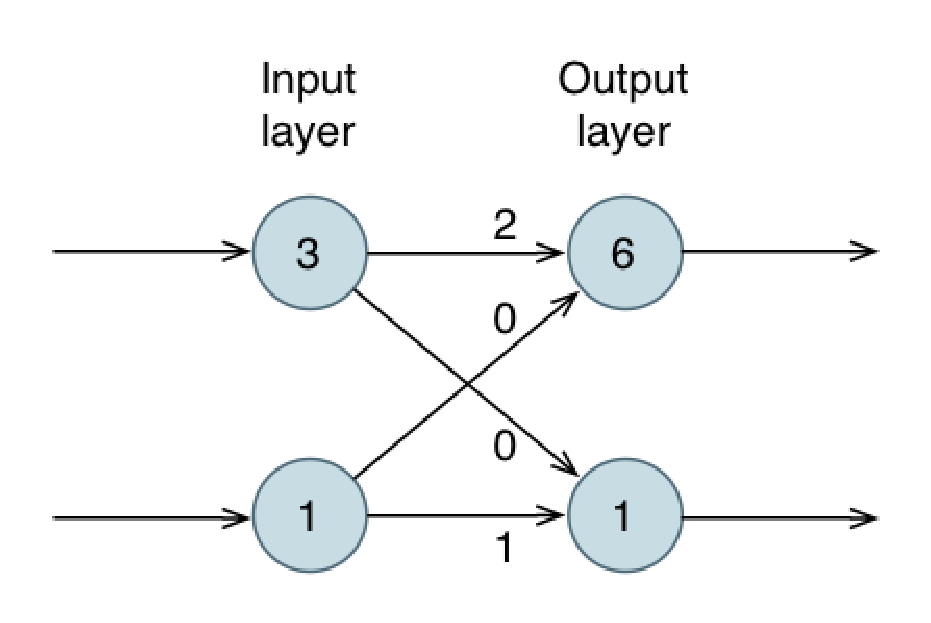
\includegraphics[height=4cm,
    angle=0]{./images/lineartransform_neuralnet.eps},
    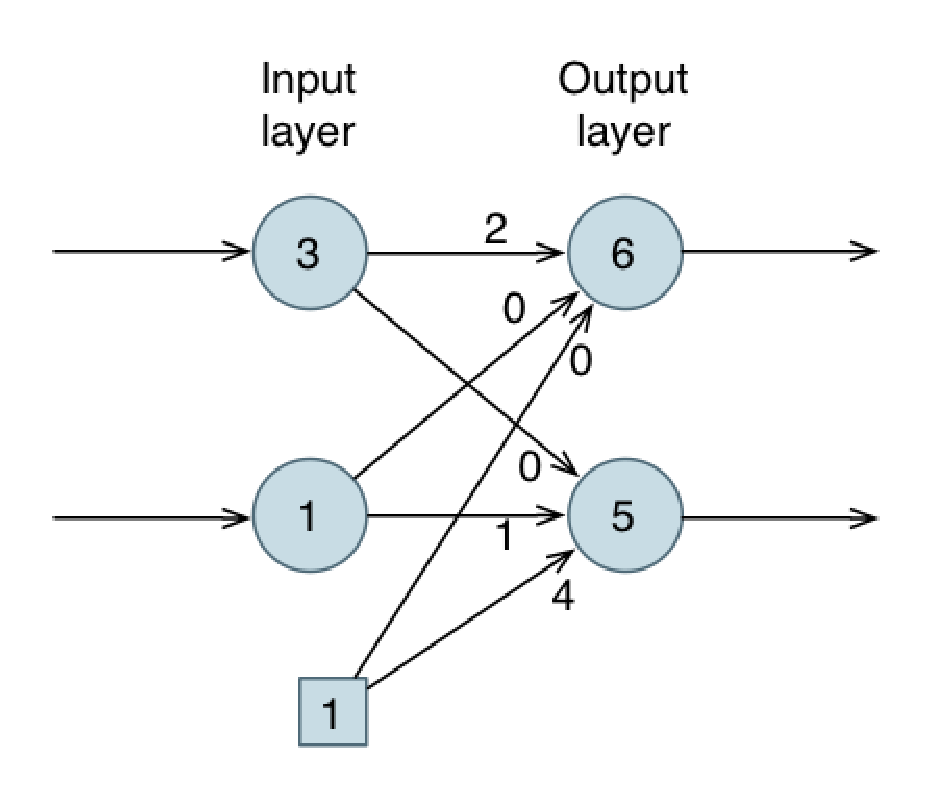
\includegraphics[height=4cm,
    angle=0]{./images/lineartransform_neuralnet_with_bias.eps}}
\caption{(A) Linear transform the neural network way (simple); (B) using Bias vector}
\label{fig:lineartransform_neuralnet}
\end{figure}

In practice, we use affine transformation (Sect.\ref{sec:affine-transformation})
more often in neural network, with $\mathbf{b}$ represents a bias to achieve
some form of {\bf non-linearity}. It means that if the input is zero, we have a
confident that it should belong to a given output class based on the given bias.
Bias vector is also a hyper-parameter.

Consider the bias vector $\mathbf{b} = [0, 4]^T$. Here, the bias is only applied
to the second unit in the output layer, i.e.
the first element of the bias vector is zero; and only the non-zero elements
impose a bias on the output. Using this, we can achieve some form of
non-linearity.

A more real nonlinearity is need to achieve more complicated transformation, and
thus can achieve better learning of a neural network. The idea is that instead
of treating the result of the affine transformation as the output of the node,
we add an additional step, i.e. running the linear combination through a
nonlinear activation function and treating that as the unit output.

There are a whole bunch of different options available for which activation
function you use (Sect.\ref{sec:activation-function-nonlinearity}).

\subsection{sparse matrix}
\label{sec:math-sparse-matrix}

It is common that the matrix $\mathbf{A}$ is sparse, which is to say that it
contains only a small number of non-zero values.

Even if A was a 1 million by 1 million matrix with only 5 million non-zero
entries (and thus we need only store those 5 million), the inverse will
typically have almost every entry non-negative, requiring us to store all 1M -
$\times$ -  1M  entries—that is 1 trillion entries!


There are multiple data structures that can be used to efficiently construct a sparse matrix; three common choices
\begin{enumerate}
  \item  Dictionary of Keys. A dictionary is used where a row and column index is mapped to a value.
  
  \item List of Lists. Each row of the matrix is stored as a list, with each sublist containing the column index and the value.
 
  
  \item Coordinate List. A list of tuples is stored with each tuple containing the row index, column index, and the value.
\end{enumerate}

However, for performing efficient operations, there are different choices of
data structures that are more suitable
\begin{enumerate}
  
  \item Compressed Sparse Row (CSR). The sparse matrix is represented using three
  one-dimensional arrays for the non-zero values, the extents of the rows, and
  the column indexes.
  
 \textcolor{red}{CSR is often used to represent sparse matrices in machine
 learning given the
  efficient access and matrix multiplication that it supports.}
  
  \item Compressed Sparse Column. The same as the Compressed Sparse Row method
  except the column indices are compressed and read first before the row
  indices.
  
\end{enumerate}

In Python, the CSR form of a sparse matrix is created using \verb!scipy.sparse.csr_matrix!
\begin{lstlisting}


# dense to sparse
from numpy import array
from scipy.sparse import csr_matrix
# create dense matrix
A = array([[1, 0, 0, 1, 0, 0], [0, 0, 2, 0, 0, 1], [0, 0, 0, 2, 0, 0]])
print(A)

# convert to sparse matrix (CSR method)
S = csr_matrix(A)
print(S)

# reconstruct dense matrix
B = S.todense()
print(B)


from numpy import count_nonzero

sparsity = 1.0 - count_nonzero(A) / A.size

\end{lstlisting}

The number of non-zero elements in a NumPy array can be given by the \verb!count_nonzero()! function


\subsection{-- in deep learning}


Sparse matrices come up in encoding schemes used in the preparation of data.
\begin{enumerate}
  \item One-hot encoding, used to represent categorical data as sparse binary vectors. 
  
  The output layer with the number of units represent the number of categories, the vector represent one category 
  is a one-hot vector, e.g. one element is zero and all other elements are zeroes. Category-1 is represented by 
  $\mathbf{l} = [1,0,0,\ldots,0]$.
  
  \verb!sklearn.preprocessing.OneHotEncoder! encode categorical features as a one-hot numeric array.
  \url{https://scikit-learn.org/stable/modules/generated/sklearn.preprocessing.OneHotEncoder.html}
  
  \item Count encoding, used to represent the frequency of words in a vocabulary for a document
  
  Suppose there are $n$ words, the vector represent the frequency of all words
  (in a paragraph or a sentence) is represented by $\mathbf{f}= (f_1, f_2,
  \ldots, f_n)$; in that $f_i$ is the frequency of $i$-th word. This is typically a sparse vector.
  
\begin{verbatim}

If there are 100,000 words in the language model, then the feature vector has
length 100,000, but for a short email message almost all the features will have
count zero.
\end{verbatim}

  The minibatch, i.e. a subset of training samples is then represented by a matrix, in that each row is a sparse vector, so 
  the matrix itself is also a sparse matrix.
  
  \verb!sklearn.feature_extraction.text.CountVectorizer! convert a collection of text documents to a matrix of token counts.
  \url{https://scikit-learn.org/stable/modules/generated/sklearn.feature_extraction.text.CountVectorizer.html}
  
  \item TF-IDF encoding, used to represent normalized word frequency scores in a vocabulary.
 
 \verb!sklearn.feature_extraction.text.TfidfVectorizer! convert a collection of raw documents to a matrix of TF-IDF features.
 This is equivalent to CountVectorizer followed by TfidfTransformer.
 
\end{enumerate}

We often need sparse matrix in 
\begin{itemize}	 
  \item  Natural language processing for working with documents of text.
  
  \item Recommender systems for working with product usage within a catalog.
  
  \item Computer vision when working with images that contain lots of black pixels.
\end{itemize}
 
\subsection{Rank of a matrix: linear dependence vs linear independent}
\label{sec:math-matrix-rank}

If we have a general $n-\times-m$ matrix, it is reasonable to ask what dimension
space the matrix maps into.

Some distortions can be severe, e.g. the matrix below compresses the entire
two-dimensional plane down to a single line. This is the example when using a
matrix that has a column is a linear dependence of other columns. In this case,
we call the {\bf rank} of the $n-\times-n$ matrix is lower than $n$.
\begin{equation}
\mathbf{B} = \begin{bmatrix}
2 & -1 \\ 4 & -2
\end{bmatrix},
\end{equation}


\textcolor{red}{A criteria to test of a matrix is of rank} $n$: given the column
vectors are $v_1, \ldots, v_n$; and if there exist coefficients
 $a_1, \ldots, a_n$ not all equal to zero so that
\begin{equation}
\sum_i a_i \mathbf{v}_i = 0
\end{equation}
then the rank must be lower than $n$. 
This procedure, as described, is very inefficient.
It requires looking at every subset of the columns of our given matrix,
and thus is potentially exponential in the number of columns.
\textcolor{red}{Using determinant is a better choice to test the rank} (Sect.\ref{sec:math-matrix-determinant}).

\textcolor{red}{In Python: we use} \verb!numpy.linalg.matrix_rank!, or
\begin{lstlisting}{lang="python"}
def rank(A, eps=1e-12):
    u, s, vh = numpy.linalg.svd(A)
    return len([x for x in s if abs(x) > eps])
\end{lstlisting}

NOTE: \verb!eps! depends in your application - most would agree that 1e-12
corresponds to zero, but you may witness numerical instability even for
\verb!eps=1e-9!.


In particular, the rank of a matrix $\mathbf{A}$ is the largest number of
linearly independent columns amongst all subsets of columns.
The matrix $\mathbf{B}$ above  has \verb!rank(B)! = 1, since the two columns are
linearly dependent, but either column by itself is not linearly dependent.


If a matrix is of rank $n$, i.e. there is no linear dependence, we say the
(column) vectors are linearly independent.

\subsection{Rank vs. SVD}

Suppose a $N\times M$ matrix, and the Singular Value Decomposition (SVD -
Sect.\ref{sec:SVD}) of that matrix $\mathbf{W}$ is
\begin{equation}
\mathbf{W} = \mathbf{U. \Sigma. V^T}
\end{equation}
with $\nu_i = \Sigma_{ii}$ the diagonal element of the matrix $\Sigma$.

The Matrix Rank, or Hard Rank, is simply the number of non-zero singular values
($\nu_i > 0$), i.e. number of non-zero diagonal of the matrix $\Sigma$.

\begin{equation}
\mathcal{R}(\mathbf{W}) = \sum \delta(\nu_i > 0)
\end{equation}

Of course, being a numerical method, we really mean the number of singular
values above some tolerance ($\nu_i > $epsilon) and we can get different results
depending on if we use (either Python default tolerance (epsilon), or numerical recipes
tolerance which is tighter).
\begin{lstlisting}{lang="python"}
def rank(A, eps=1e-12):
    u, s, vh = numpy.linalg.svd(A)
    return len([x for x in s if abs(x) > eps])
\end{lstlisting}



\subsection{Full Rank (=n) vs. Singular matrix (< $n$)}

If all the singular values are non-zero, we say $\mathbf{W}$  is Full Rank. If one
or more $\nu_{i}\sim 0$, then we say $\mathbf{W}$  is Singular.

A Singular matrix has lost expressiveness, and the model has undergone Rank collapse.

\subsection{-- Fixing Rank Collapse: Tikhonov Regularization}

When a model undergoes Rank Collapse, it means multiple input will be mapped to
the same output, i.e. label. This is NOT good.
So, it traditionally needs to be regularized, i.e. we add some small constant
$\gamma$ to the diagonal of the matrix $\mathbf{W}$. This procedure is also
called {\bf Tikhonov Regularization}.  
\begin{equation}
\mathbf{W^T.W} = \mathbf{W^T.W} + \gamma \gamma
\end{equation}

\begin{mdframed}

In cases where $\mathbf{W}$  is Singular, regularization is absolutely necessary.
But even when it is not singular, Regularization can be useful in traditional
machine learning.

\end{mdframed}

So that all the singular values will now be greater than zero, and we can form a
generalized pseudo-inverse, called the {\bf Moore-Penrose Inverse}
(Sect.\ref{sec:Moore-Penrose-inverse}).
\begin{equation}
\mathbf{W}^\dagger = (\mathbf{W^T.W} + \gamma \gamma)^{-1}
\end{equation}

The constant, or Regularizer, $\gamma$ 
sets the Noise Scale for the model.
\begin{enumerate}
  \item {\bf Information}: stays in the singular vector associated with largest singular values $\nu_i > \gamma$
  
  
  \item {\bf Noise}: stays in the singular vector where $\nu_i < \gamma$
\end{enumerate}


\url{https://calculatedcontent.com/2018/09/21/rank-collapse-in-deep-learning/}

\subsection{-- Moore-Penrose Inverse (Generalized Inverse)}
\label{sec:Moore-Penrose-inverse}

Moore-Penrose is the technique for finding the inverse of a rectangular matrix
generalized from square matrix. It is called Moore-Penrose Inverse after two
independent discoverers of the method or the Generalized Inverse.

$m-\times-n$ matrix $\mathbf{A}$. Given \verb!A=V.Sigma.U^T!, the pseudoinverse
is calculated using the singular value decomposition of A:

\begin{verbatim}
A^+ = V . Sigma^+ . U^T
\end{verbatim}

NOTE: U and V can be retrieved from SVD operation. 
For the diagonal matrix, the transpose is the reciprocal of every diagonal elements.
\begin{verbatim}
Sigma^+ = [   1/s11, 0, \ldots 0 
              0     1/s22, \ldots, 0
              \ldots
              0 , \ldots, 1/snn    ]
\end{verbatim}

IMPORTANCE:  The pseudoinverse provides one way of solving the linear regression
equation, specifically when there are more rows than there are columns, which is
often the case.

In Python: NumPy has \verb!pinv()!
\begin{lstlisting}
from numpy.linalg import pinv
# define matrix
A = array([
	[0.1, 0.2],
	[0.3, 0.4],
	[0.5, 0.6],
	[0.7, 0.8]])
print(A)
# calculate pseudoinverse
B = pinv(A)
\end{lstlisting}


\subsection{Rank vs. Determinant}
\label{sec:math-matrix-determinant}

A square matrix is full rank if and only if its determinant is nonzero.

Let $\mathbf{A}$ be an $n-\times-n$ matrix, note that \verb!det(A)! $\ne$ 0 det
\verb!iff! the rows are linearly independent iff \verb!rank(A)=n!.

\begin{lstlisting}{lang="python"}
import numpy as np

mat = np.array([[1, -1], [2, 3]])
np.linalg.det(mat)
\end{lstlisting}

Finding number of non-zero eigenvalues is the rank of a matrix (Sect.\ref{sec:eigendecomposition-usage}).

The determinant can be positive, negative, or zero. 

Computing determinants for larger matrices can be laborious, but the intuition
is the same. The determinant remains the factor that $n-\times-n$ matrices scale
n-dimensional volumes (Sect.\ref{sec:math-linear-transformation}).


\subsection{linear dependence = compress the space}

If the columns of a matrix are linearly independent, no compression occurs and
the operation can be undone.

A linear dependence in the columns of a matrix is a witness to the fact that our
matrix is compressing the space down to some lower dimension.

\subsection{Special matrices: I (identity matrix)}

The {\bf identity matrix} is the matrix with ones along the diagonal, and zeros elsewhere. 
The linear transformation using $\mathbf{I}$ leaves our data unchanged when applied.

This is equivalent to applying to a rank-n matrix $\mathbf{A}$, and then apply
the transformed point to the inverted matrix $\mathbf{A}^{-1}$.

\begin{equation}
\mathbf{A^{-1}  A=AA^{-1} =I.}
\end{equation} 


\subsection{Matrix norm (Frobenius norm)}
\label{sec:math-norm-matrix}


This is equivalent to take the L2 norm of the matrix after flattening, i.e.
turns the matrix into a vector and L2-norm of that vector.

\begin{equation}
||\mathbf{A}||_F = \sqrt{\sum_{i,j}A^2_{i,j}}
\end{equation}


We can use \verb!numpy.linalg.norm(A)!




\section{Hyperplanes}
\label{sec:math-hyperplane}

A hyperplane split the space (of n-dimension) into 2 parts. 

{\bf Hyperplane}, a generalization to higher dimensions of a line (two
dimensions) or of a plane (three dimensions). In an $n$-dimensional vector
space, a hyperplane has $d-1$ dimensions and divides the space into two
half-spaces.


Recall the question we have in Sect.\ref{sec:math-dot-product-vectors}, what are
the points $v$ such that its dot product with a given vector $w$ is 1, i.e.  $w
\cdot v=1$.
Consider $w=[2,1]^T$. \textcolor{red}{IMPORANT: 1 is just a value of choice, and
we call it a threshold}.

The dot product, can be written as 
\begin{equation}
||v|| ||w|| \cos(\theta) = 1
\end{equation}
or
\begin{equation}
||v||  \cos(\theta) = \frac{1}{||w||} = \frac{1}{\sqrt{5}}
\end{equation}

This is equivalent to saying that the length of the projection of $v$ onto the
direction of $w$ is exactly $\frac{1}{||w||}$.

The set of all points where this is true is a line, satisfying the equation
$2x+y=1$.


If we now look at what happens when we ask about the set of points with
\begin{equation}
v \cdot w < 1
\end{equation}
or
\begin{equation}
v \cdot w > 1
\end{equation}
Those two inequalities define either side of the line.

\begin{itemize}
  \item  If, $u$ and $w$ are 3-dimensional vector, then the line becomes a plane. 

  \item If, $u$ and $w$ are n-dimensional vector, then the line becomes a hyperplane of (n-1) dimensions. 
  
\end{itemize}

\subsection{Hyperplane as decision plane}

In ML, where data samples are represented as points (vectors), such hyperplanes
are often referred to as decision planes. 

The majority of deep learned classification models end with a linear layer fed
into a softmax, so one can interpret the role of the deep neural network to be
to find a non-linear embedding such that the target classes can be separated
cleanly by hyperplanes.

\subsection{A crude classifier using hyperplane}
\label{sec:math-hyperplane-threshold}

A classifier, e.g. hyperplane, that can classify tiny images of t-shirts and
trousers from the Fashion MNIST dataset.
\begin{lstlisting}{lang=python}
# Load in the dataset
train = gluon.data.vision.FashionMNIST(train=True)
test = gluon.data.vision.FashionMNIST(train=False)

# each row is a two-element vector, 
#   x[0] = sample
#   x[1] = label
X_train_0 = np.stack([x[0] for x in train if x[1] == 0]).astype(float)
X_train_1 = np.stack([x[0] for x in train if x[1] == 1]).astype(float)

X_test = np.stack(
    [x[0] for x in test if x[1] == 0 or x[1] == 1]).astype(float)
y_test = np.stack(
    [x[1] for x in test if x[1] == 0 or x[1] == 1]).astype(float)

\end{lstlisting}
In Python: \verb!numpy.stack()! function is used to join a sequence of same
dimension arrays along a new axis. By default, \verb!iterator! iterates by row. 

The mean point in each group is calculated, $u$ and $w$ respectively. The two
points form a vector, $v=u-w$.
\begin{lstlisting}{lang=python}
# Compute averages
ave_0 = np.mean(X_train_0, axis=0)
ave_1 = np.mean(X_train_1, axis=0)


# Plot average t-shirt
d2l.set_figsize()
d2l.plt.imshow(ave_0.reshape(28, 28).tolist(), cmap='Greys')
d2l.plt.show()

# Plot average trousers 
d2l.plt.imshow(ave_1.reshape(28, 28).tolist(),
cmap='Greys') d2l.plt.show()
\end{lstlisting}
The mean point itself is also an image. In this case, when we plot the two mean
points, they shows two blurry images of a t-shirt, and a trousers.

Here, taking the vector between their means to define the decision plane and
eyeball a crude threshold The average is itself an image, which in this case
indeed resembles a blurry image of a t-shirt.
 
Using the mean points, the difference forms a row vector, $v=u-w$; so we take
the transform to get a column vector
\begin{lstlisting}{lang=python}
# Print test set accuracy with eyeballed threshold
w = (ave_1 - ave_0).T
\end{lstlisting}

Now, we find a hyperplane that is best at splitting the points in each group.
The choice of this hyperplane is given by the choice of the threshold value
$t=-1500000$.

Example: 
\begin{lstlisting}{lang=python}
predictions = X_test.reshape(2000, -1).dot(w.flatten()) > -1500000

# Accuracy
np.mean(predictions.astype(y_test.dtype) == y_test, dtype=np.float64)
\end{lstlisting}


\subsection{SVM}
\label{sec:math-hyperplane-SVM}

Support Vector Machine (SVM) provides a strategy for finding the right
hyperplane. The plane is chosen based on the choices of a number of points
called {\bf support vectors}.


Support Vector Machine is a linear model for classification and regression
problems. It can solve linear and non-linear problems and work well for many
practical problems. The idea of SVM is simple: The algorithm creates a line or a
hyperplane which separates the data into classes.
 
 
\section{Tensor}
\label{sec:tensor}

We have worked with vector, matrix.
Rather treating each differently, a unified view on a number of matrix and
vector operations is provided via {\bf tensor}. 

In matrix multiplication, $\mathbf{C = A B}$, the formula to find elements of $\mathbf{C}$ is
\begin{equation}
c_{i, j} = \sum_{k} a_{i, k}b_{k, j}.
\end{equation}

With tensor, a generalized formula is used, in that user needs to specify the coefficients
\begin{equation}
y_{il} = \sum_{jk} x_{ijkl}a_{jk}.
\end{equation}
Such a transformation is called a {\bf tensor contraction.}
This represents a far more flexible family of transformations
that matrix multiplication alone.

\begin{mdframed}
Simplified math notation: Einstein notation,
where the summation is implicitly taken over all repeated indices.

\begin{equation}
y_{il} = x_{ijkl}a_{jk}.
\end{equation}
\end{mdframed}

{\bf Tensor notations}:
\begin{enumerate}
  \item  $\mathbf{v} \cdot \mathbf{w} = \sum_i v_iw_i$
\item  $\|\mathbf{v}\|_2^{2} = \sum_i v_iv_i$
\item  $(\mathbf{A}\mathbf{v})_i = \sum_j a_{ij}v_j$
\item  $(\mathbf{A}\mathbf{B})_{ik} = \sum_j a_{ij}b_{jk}$
\item  $\mathrm{tr}(\mathbf{A}) = \sum_i a_{ii}$
\end{enumerate}

In Python
\begin{lstlisting}{lang="python"}
# Define tensors
B = np.array([[[1, 2, 3], [4, 5, 6]], [[7, 8, 9], [10, 11, 12]]])
A = np.array([[1, 2], [3, 4]])
v = np.array([1, 2])

# Print out the shapes
A.shape, B.shape, v.shape
\end{lstlisting}




\chapter{Eigendecomposition: eigenvalue + eigenvector}
\label{sec:eigendecomposition}

We have learnt {\bf matrix } (Sect.\ref{sec:math-matrix}), and linear transformation (Sect.\ref{sec:math-linear-transformation}).

Matrix decomposition, also known as matrix factorization, involves describing a given matrix using its constituent elements.
\begin{enumerate}

  \item Eigendecomposition refers to a technique that we rewrite the given matrix in its
new form (Sect.\ref{sec:decomposition-matrix}) using eigenvalues and
eigenvectors.
  
  \item  SVD is a matrix decomposition technique (Sect.\ref{sec:SVD}).

All matrices have an SVD, which makes it more stable than other methods, such as
the eigendecomposition.

\end{enumerate}



Suppose matrix $\mathbf{A}$
\begin{equation}
\mathbf{A} = \begin{bmatrix}
2 & 0 \\
0 & -1
\end{bmatrix}.
\end{equation}

which transforms a vector $\mathbf{v} = [x, y]^\top$ to a new one $\mathbf{v}A =
[2x, -y]^\top$.

Typically, this transformation is applied to every dimension.
Namely $[1, 0]^\top$ gets sent to $[2, 0]^\top$ and $[0, 1]^\top$ gets sent to
$[0, -1]^\top$.  An intuitive interpretation is that the transformation stretch
the vector to be twice as wide in the $x$-direction, and then flip it in the
$y$-direction.


However, there are some vectors for which something remains unchanged, i.e. it
changes homogeneously to every element (or geometrically, it does not change the
direction of the vector). The transformed vectors are still in the same line of
the origin vectors. \textcolor{red}{This is an interesting property} as we will
discover here.


If  $\mathbf{A}$ is fixed, in general, we can find a number 
$\lambda$ and a vector 
$\mathbf{v}$  such that
\begin{equation}
\mathbf{A. v} = \lambda \mathbf{v}
\end{equation}
It means that matrix $\mathbf{A}$ applied to the vector $\mathbf{v}$ only scale the vector with a
coefficient $\lambda$. In Python it means \verb!dot(a,v) = w * v!

In the above example, $\lambda = 2$ when $\mathbf{v} = [1,0]^\top$.

We say that $\mathbf{v}$ is an eigenvector and $\lambda$ is an
eigenvalue for matrix $\mathbf{A}$.

\section{Eigenvalue: how to find}

REMEMBER: using the fact that the eigenvalues of a diagonal matrix are its
diagonal elements. 
Efficient, accurate methods to compute eigenvalues and eigenvectors of arbitrary
matrices were not known until the QR algorithm was designed in 1961.

We solve the equation
\begin{equation}
(\mathbf{A} - \lambda \mathbf{I})\mathbf{v} = 0
\end{equation}

We see that  $\mathbf{A- \lambda I)}$
must compress some direction down to zero,
hence it is not invertible, and thus the determinant is zero.

Thus, we can find the *eigenvalues* by finding for what $\lambda$ is
$\det(\mathbf{A}-\lambda \mathbf{I}) = 0$. This is discussed in
Sect.\ref{sec:math-matrix-determinant}.
Solving this polynomial equation returns all values of $\lambda$.


Python provides the code
\begin{enumerate}
  
  \item   \verb!numpy.linalg.eigvals()! method; or \verb!scipy.linalg.eigvals()!
  
  based on \verb!_geev! LAPACK routines which compute the eigenvalues and eigenvectors of general square arrays.
  
  \item or \verb!numpy.linalg.eig()!: return eigenvalue (w), and eigenvector (v); 
  or \verb!scipy.linalg.eig()!
  
  also based on \verb!_geev! LAPACK.
  
  NOTE: SciPy contains more fully-featured versions of the linear algebra
  modules, as well as many other numerical algorithms.
  
\end{enumerate}


\begin{lstlisting}{lang="python"}
%matplotlib inline
import d2l
from IPython import display
import numpy as np
from numpy import linalg as LA

w, v = LA.eig(np.array([[2, 1], [2, 3]]))

w = np.linalg.eigvals(np.array([[2, 1], [2, 3]]))


# Compute the eigenvalues
eigs = np.linalg.eigvals(A).tolist()
\end{lstlisting}

NOTE: Note that numpy normalizes the eigenvectors to be of length one,
whereas we took ours to be of arbitrary length.
Additionally, the choice of sign is arbitrary.

Eigenvalues are often difficult to reason with intuitively.
If presented an arbitrary matrix, there is little that can be said about what
the eigenvalues are without computing them. There are a number of theorems that
can provide some insights without computing them.
\begin{enumerate}
  \item Gershgorin Circle Theorem (Sect.\ref{sec:Gershgorin-Circle-Theorem})
\end{enumerate}

The largest eigenvalue of a matrix is aka {\bf principle eigenvalue} (Sect.\ref{sec:principle-eigenvalue}).

\subsection{Gershgorin Circle Theorem}
\label{sec:Gershgorin-Circle-Theorem}

If the exact value of eigenvalues are not important, i.e. an approximated value
is good enough, we can avoid the expensive computation to calculate the
eigenvalues. The {\bf Gershgorin Circle Theorem} can provide approximate values for
the eigenvalues of a matrix.



Let $\mathbf{A} = (a_{ij})$ be any square matrix ($n\times n$).
We will define $r_i = \sum_{j \neq i} |a_{ij}|$.
Let $\mathcal{D}_i$ represent the disc in the complex plane 
with center $a_{ii}$ radius $r_i$.
Then, every eigenvalue of $\mathbf{A}$ is contained in one of the $\mathcal{D}_i$.


Example to explain the theorem: Consider this matrix

\begin{equation}
\mathbf{A} = \begin{bmatrix}
1.0 & 0.1 & 0.1 & 0.1 \\
0.1 & 3.0 & 0.2 & 0.3 \\
0.1 & 0.2 & 5.0 & 0.5 \\
0.1 & 0.3 & 0.5 & 9.0
\end{bmatrix}.
\end{equation}

The four radius are:  $r_1 = 0.3$, $r_2 = 0.6$, $r_3 = 0.8$ and $r_4 = 0.9$.

This means that all of our eigenvalues will be in one of the ranges of 

$$[a_{11}-r_1, a_{11}+r_1] = [0.7, 1.3], $$

$$[a_{22}-r_2, a_{22}+r_2] = [2.4, 3.6], $$

$$[a_{33}-r_3, a_{33}+r_3] = [4.2, 5.8], $$

$$[a_{44}-r_4, a_{44}+r_4] = [8.1, 9.9]. $$


To double check, we compute the four eigenvalues
\begin{lstlisting}
A = np.array([[1.0, 0.1, 0.1, 0.1],
              [0.1, 3.0, 0.2, 0.3],
              [0.1, 0.2, 5.0, 0.5],
              [0.1, 0.3, 0.5, 9.0]])

v, _ = np.linalg.eig(A) 
v
\end{lstlisting}

The eigenvalues are approximately 0.99, 2.97, 4.95, 9.08, all comfortably inside
the ranges provided.


\textcolor{red}{\bf What does it means?} If the diagonal $a_{ii}$ is
significantly larger than all the other elements, it means the range will be
small; which enables the approximations of eigenvalues will be fairly accurate.





\section{Eigenvector: how to find}

Eigenvectors are vectors which are stretched by a matrix without changing
direction. Eigenvalues are the amount that the eigenvectors are stretched by the
application of the matrix. 

Once we find the eigenvalues, we can solve 
$\mathbf{A}\mathbf{v} = \lambda \mathbf{v}$ 
to find the associated *eigenvector(s)*.

All the eigenvetors can be written as column vectors of a matrix
\begin{equation}
\mathbf{W} = \begin{bmatrix}
1 & 1 \\
-1 & 2
\end{bmatrix},
\end{equation}
be the matrix where the columns are the eigenvectors of the matrix $\mathbf{A}$.

Efficient, accurate methods to compute eigenvalues and eigenvectors of arbitrary
matrices were not known until the QR algorithm was designed in 1961. Combining
the Householder transformation with the LU decomposition results in an algorithm
with better convergence than the QR algorithm.


It is not always possible to find enough linearly independent eigenvectors. To
handle such matrices, we require more advanced techniques than we can cover
(such as the Jordan Normal Form, or Singular Value Decomposition).

\subsection{Jordan Normal Form}

Jordan Normal Norm is an advanced technique to find eigenvalues and eigenvectors.


\section{Singular Value Decomposition (SVD)}
\label{sec:SVD}


All matrices have an SVD, which makes it more stable than other methods, such as the eigendecomposition.

With SVD, it turns a matrix into other matrices such that it makes certain
subsequent matrix calculations simpler.
\begin{lstlisting}
A = U . Sigma . V^T
\end{lstlisting}
\begin{itemize}
  \item A : $m-\times-n$ real matrix
  
  \item U: $m-\times-m$ matrix
 
 The columns of the U matrix are called the left-singular vectors of A
  
  \item Sigma: $m-\times-n$ diagonal matrix
  
  The diagonal values in the Sigma matrix are known as the singular values of the original matrix A. 
  
  \item $V^T$: the  transpose of an n x n matrix 

 The columns of V are called the right-singular vectors of A.
 
\end{itemize}

The SVD is calculated via iterative numerical methods.

\begin{mdframed}

Every rectangular matrix has a singular value decomposition, although the
resulting matrices may contain complex numbers and the limitations of floating
point arithmetic may cause some matrices to fail to decompose neatly.

The SVD allows us to discover some of the same kind of information as the
eigendecomposition. However, the SVD is more generally applicable.

The SVD is used widely both in the calculation of other matrix operations, such
as matrix inverse, but also as a data reduction method in machine learning. SVD
can also be used in least squares linear regression, image compression, and
denoising data.

\end{mdframed}

In Python
\begin{lstlisting}
from numpy import array
from scipy.linalg import svd

A = array([[1, 2], [3, 4], [5, 6]])

# SVD
U, s, VT = svd(A)
\end{lstlisting}

IMPORTANT: The U, s, and V elements returned from the svd() cannot be multiplied directly.
\begin{itemize}
  \item  The s vector must be converted into a diagonal matrix using the diag() function.
  
  By default, it creates a square matrix that is n x n, relative to our original matrix.
  However, what we need is a $m-\times-n$ matrix. 
  
  We can achieve this by creating a new Sigma matrix of all zero values that is
  m x n (e.g. more rows) and populate the first n x n part of the matrix with
  the square diagonal matrix calculated via diag().
\begin{lstlisting}
from numpy import diag

# create m x n Sigma matrix
Sigma = zeros((A.shape[0], A.shape[1]))
# populate Sigma with n x n diagonal matrix
Sigma[:A.shape[1], :A.shape[1]] = diag(s)
\end{lstlisting}
  
  \item Reconstruct the matrix
\begin{verbatim}
from numpy import dot

# reconstruct matrix
B = U.dot(Sigma.dot(VT))
\end{verbatim}
\end{itemize}

\section{Eigendecomposition: matrix decomposition into eigenvalues + eigenvectors}
\label{sec:decomposition-matrix}

The eigenvalues can also be written in matrix form, i.e. a diagonal matrix in that eigenvalues resides on the diagonal line.
\begin{equation}
\boldsymbol{\Sigma} = \begin{bmatrix}
1 & 0 \\
0 & 4
\end{bmatrix},
\end{equation}
be the matrix with the associated eigenvalues on the diagonal.

Then, collectively, we can write in matrix form 
\begin{equation}
\mathbf{A}\mathbf{W} =\mathbf{W} \boldsymbol{\Sigma} .
\end{equation}


The matrix $W$ is invertible, so we may multiply both sides by $W^{-1}$ on the right,
\begin{equation}
\mathbf{A} = \mathbf{W} \boldsymbol{\Sigma} \mathbf{W}^{-1}.
\end{equation}

Such a decomposition of matrix $\mathbf{A}$ will exist as long as we can find a
full collection of linearly independent eigenvectors (so that W is
invertible). We will learn there are nice consequences of this (Sect.\ref{sec:eigendecomposition-usage}).

\subsection{Symmetric matrix}


The most commonly encountered family are the *symmetric matrices*,
which are those matrices where $\mathbf{A} = \mathbf{A}^\top$. 

We may take $W$ to be an *orthogonal matrix*—a matrix whose columns are all
length one vectors that are at right angles to one another, where
$\mathbf{W}^\top = \mathbf{W}^{-1}$—and all the eigenvalues will be real.

\begin{equation}
\mathbf{A} = \mathbf{W}\boldsymbol{\Sigma}\mathbf{W}^\top .
\end{equation}




\section{The importance of eigendecomposition}
\label{sec:eigendecomposition-usage}

Eigendecompositions can simplify many linear-algebraic computations
and are a fundamental operation underlying many numerical algorithms
and much of the analysis that we do in linear algebra.

The eigendecomposition of a matrix can allow for many operations to be reduced
to operations on the eigenvalues.

We can 
\begin{enumerate}
  \item compute the positive power of a matrix just by raing the eigenvalues to the same power.
  
\begin{equation}
\mathbf{A}^n = \overbrace{\mathbf{A}\cdots \mathbf{A}}^{\text{$n$ times}} = \overbrace{(\mathbf{W}\boldsymbol{\Sigma} \mathbf{W}^{-1})\cdots(\mathbf{W}\boldsymbol{\Sigma} \mathbf{W}^{-1})}^{\text{$n$ times}} =  \mathbf{W}\overbrace{\boldsymbol{\Sigma}\cdots\boldsymbol{\Sigma}}^{\text{$n$ times}}\mathbf{W}^{-1} = \mathbf{W}\boldsymbol{\Sigma}^n \mathbf{W}^{-1}.
\end{equation}
  
  For any positive power of a matrix, the eigendecomposition is obtained by just raising the eigenvalues to the same power.

  \item invert the matrix just by inverting the eigenvalues

\begin{equation}
\mathbf{A}^{-1} = \mathbf{W}\boldsymbol{\Sigma}^{-1} \mathbf{W}^{-1},
\end{equation}

This will work as long as each eigenvalue is non-zero, so we see that invertible
is the same as having no zero eigenvalues.

  \item quickly compute the determinant of a matrix (Sect.\ref{sec:math-matrix-determinant}) 

If $\lambda_1, \ldots, \lambda_n$ 
are the eigenvalues of a matrix, then the determinant of that matrix is
\begin{equation}
\det(\mathbf{A}) = \lambda_1 \cdots \lambda_n,
\end{equation}

This makes sense intuitively because whatever stretching $\mathbf{W}$ does,
$W^{-1}$ undoes it, so in the end the only stretching that happens is by
multiplication by the diagonal matrix $\boldsymbol{\Sigma}$, which stretches
volumes by the product of the diagonal elements.

  \item compute the rank (Sect.\ref{sec:math-matrix-rank}) which is the same as
  the number of non-zero eigenvalues of $\mathbf{A}$.

\end{enumerate}

\section{Eigenvalues/Eigenvectors in traditional ML}


In linear methods from unsupervised learning (e.g. factor analysis also known as
Principal Component Analysis) and supervised learning (e.g. discriminant
analysis) eigenvectors are used.

In factor analysis (Principal Component Analysis, PCA), we take the Covariance
matrix and we try to represent our data set in a new coordinate system that is
transformed.

Imagine you have images (which are high dimensional) as inputs. The goal is to
find a new coordinate system which captures a maximal amount of variance in the
images.

\url{https://math.stackexchange.com/questions/3153522/why-are-eigenvectors-important-for-deep-learning-applications}


\section{Eigenvalues/Eigenvectors in Deep Learning}
\label{sec:deep-learing-mathematical-intuition-init-weights}

Eigenvectors are not so important in deep learning. Deep learning is using
highly nonlinear transformations. That is why concepts from linear algebra like
eigenvalues and eigenvectors do not play a major role in this field.

There might be other fields in machine learning where eigenvalues and
eigenvectors are important. But the core of deep learning relies on nonlinear
transformations. Eigenvalues and eigenvectors are a core concept from linear
algebra but not for the description of nonlinear transformations.
 

\textcolor{red}{In deep neural net, we will see that mathematically, an input
vector is mapped to the output by interspersing layers
of linear transformations with non-linear operations.}

In the simple scenario, we consider only linear transformation, i.e.
a series of matrix multiplication.
\begin{equation}
\mathbf{v}_{out} = \mathbf{A_1}\cdot \mathbf{A_k}\cdots \mathbf{A_n} \mathbf{v}_{in}
\end{equation}

\textcolor{red}{REMEMBER}: The learning process is the one that adjust weights,
or elements of the matrices $\mathbf{A}_k$.

In the simplest case, for a toy model, the transformation is a single repeated matrix operation 
$\mathbf{A}$
\begin{equation}
\mathbf{v}_{out} = \mathbf{A}\cdot \mathbf{A}\cdots \mathbf{A} \mathbf{v}_{in} = \mathbf{A}^N \mathbf{v}_{in}.
\end{equation}

For simplicity in our toy model, we will assume that the data vector we feed in
$\mathbf{v}_{in}$ is a random five dimensional Gaussian vector.

\textcolor{red}{Now, the question is how we initialize values of} $\mathbf{A}$? 
A common choice is that $\mathbf{A}$ is taken to be a random matrix
with Gaussian entries.

\begin{lstlisting}{lang="python"}
np.random.seed(8675309)

k = 5
A = np.random.randn(k, k)
A
\end{lstlisting}

\textcolor{red}{The more important question is whether exist a first principle
for making the choice of initial values of } $\mathbf{A}$? Does it always result
a similar  training performance?



\subsection{The tricky part? - stretching}

For context, lets think of a generic ML problem, where we are trying to turn
input data, like an image, into a prediction, like the probability the image is
a picture of a cat.

If repeated application of $\mathbf{A}$ stretches a random vector out to be very long,
then small changes in input will be amplified into large changes in output—tiny
modifications of the input image would lead to vastly different predictions.
This does not seem right!

Example: The norm is growing uncontrollably!
\begin{lstlisting}{lang="python"}
# Calculate the sequence of norms after repeatedly applying A
v_in = np.random.randn(k, 1)

norm_list = [np.linalg.norm(v_in)]
for i in range(1, 100):
    v_in = A.dot(v_in)
    norm_list.append(np.linalg.norm(v_in))

d2l.plot(np.arange(0, 100), norm_list, 'Iteration', 'Value')
\end{lstlisting}

\subsection{The tricky part? - shrinking}

On the flip side, if $\mathbf{A}$ shrinks random vectors to be shorter, then after
running through many layers, the vector will essentially shrink to nothing, and
the output will not depend on the input. This is also clearly not right either!

\subsection{The hint in the increasing of the vector norm?}

After each matrix multiplication, we calculate the norm of the new output vector of each layer. If we take the ratio, 
and see how the norms change. 

\begin{mdframed}

\begin{lstlisting}{lang="python"}
# Compute the scaling factor of the norms
norm_ratio_list = []
for i in range(1, 100):
    norm_ratio_list.append(norm_list[i]/norm_list[i - 1])

d2l.plot(np.arange(1, 100), norm_ratio_list, 'Iteration', 'Ratio')
\end{lstlisting}

If we look at the last portion of the above computation, we see that the random
vector is stretched by a factor of 1.974459321485[...], where the portion at
the end shifts a little, but the stretching factor is stable.

\end{mdframed}


REMEMBER: We have seen that eigenvectors and eigenvalues correspond to the
amount something is stretched, but that was for specific vectors, and specific
stretches.

Now, find the eigenvalues and eigenvectors of this matrix $\mathbf{A}$.
A bit of a caveat here: it turns out that to see them all, we will need to go to
complex numbers which you can think of these as stretches and rotations.
By taking the norm of the complex number (square root of the sums of squares of
real and imaginary parts), we can measure that stretching factor.

\begin{lstlisting}{lang="python"}
# Compute the eigenvalues
eigs = np.linalg.eigvals(A).tolist()
norm_eigs = [np.absolute(x) for x in eigs]
norm_eigs.sort()
"Norms of eigenvalues: {}".format(norm_eigs)
\end{lstlisting}

\textcolor{red}{Huraaaaah}: The number we identified before for the long term
stretching of our matrix $\mathbf{A}$ applied to a random vector is *exactly*
(accurate to thirteen decimal places!) the largest eigenvalue of $\mathbf{A}$.
This is clearly not a coincidence!


This is so important that the largest eigenvalue/eigenvector is called the
*principle eigenvalue* and *principle eigenvector*.


\subsection{Input vector turned into principle eigenvector: power iteration technique}
\label{sec:principle-eigenvalue}

Consider a random vector.
This random vector points a little in every direction, so in particular, it
points at least a little bit in the same direction as the eigenvector of
$\mathbf{A}$ associated with the largest eigenvalue (aka the {\bf principle
eigenvalue}).

After applying $\mathbf{A}$, our random vector gets stretched in every possible
direction, as is associated with every possible eigenvector, but it is stretched
most of all in the direction associated with this principle eigenvector.

What this means is that after apply in $A$, our random vector is longer, and
points in a direction closer to being aligned with the principle eigenvector.

After applying the matrix many times, the alignment with the principle
eigenvector becomes closer and closer until, for all practical purposes, our
random vector has been transformed into the principle eigenvector!

\begin{mdframed}

Indeed this algorithm is the basis for what is known as the *power iteration*
for finding the largest eigenvalue and eigenvector of a matrix (Van-Loan.Golub.1983).

\end{mdframed}

\subsection{Matrix initialization in Deep Net w.r.t principle eigenvalues}
\label{sec:matrix-initialization}

The relationship between the eigenvalues (and a related object called singular
values) of random matrices has been shown to have deep connections to proper
initialization of neural networks (Pennington.Schoenholz.Ganguli.2017).

\subsection{-- Normalization matrix: principle eigenvalue = 1}
\label{sec:normalization-eigenvalue}

So, to prevent the stretching from happening, one good way is to make the {\bf principle eigenvalue} become one.
If we rescale our matrix by this principle eigenvalue so that the largest
eigenvalue is instead now just one.

\begin{lstlisting}{lang="python"}
# Rescale the matrix A
A /= norm_eigs[-1]

# Do the same experiment again
v_in = np.random.randn(k, 1)

norm_list = [np.linalg.norm(v_in)]
for i in range(1, 100):
    v_in = A.dot(v_in)
    norm_list.append(np.linalg.norm(v_in))

d2l.plot(np.arange(0, 100), norm_list, 'Iteration', 'Value')
\end{lstlisting}

So, by normalizing the matrix by its largest eigenvalue, we now can walk the
narrow line between growth and decay to make sure that our output changes
depending on our input, but not much!

Check again the ratio of vector norms
\begin{lstlisting}{lang="python"}
# Also plot the ratio
norm_ratio_list = []
for i in range(1, 100):
    norm_ratio_list.append(norm_list[i]/norm_list[i-1])

d2l.plot(np.arange(1, 100), norm_ratio_list, 'Iteration', 'Ratio')
\end{lstlisting}


After normalizing the matrices by the principle eigenvalue, we see that the
random data does not explode as before, but rather eventually equilibrates to a
specific value.

\textcolor{red}{How can we estimate this principle eigenvalue?}


\subsection{Estimate principle eigenvalue}

The largest eigenvalue of a large random $n-\times-n$ matrix with independent mean zero,
variance one Gaussian entries is on average about $\sqrt{n}$.

In the above examples, $\mathbf{A} = np.rand(5, 5)$, its largest eigenvalue is
about $\sqrt{5} = 2.2$.

This is thanks to the fascinating fact known as the {\bf circular law}
(Ginibre.1965).


\chapter{Calculus: derivative}


\section{Learning matrix's weights}
\label{sec:learning-matrix-weights}
\label{sec:deep-learing-mathematical-intuition-learn-weights}

In Sect.\ref{sec:deep-learing-mathematical-intuition-init-weights},
we have talked about the important of matrix initialization by normalizing that
matrix using principle eigenvalue (Sect.\ref{sec:matrix-initialization}). Let's
talk about learning the weights.

Suppose that we have a deep neural network where the weights (from multiple
matrices across all layers) are, for convenience, concatenated into a single
vector $\mathbf{w} = (w_1, \ldots,w_n)$.

Given a training dataset, the series of matrix transformation (across multiple
layers) produce a final output vector $\mathbf{v}_{out}$.
This vector can be different from the expected output, which we consider the
loss of our neural network on this dataset, and is written as
$\mathcal{L}(\mathbf{w})$.

This loss function is extraordinarily complex, encoding the performance of all
possible models of the given architecture on this dataset, so it is nearly
impossible to tell what set of weights $\mathbf{w}$ will minimize the loss.

The most important question is how do we find the direction which makes the
weights decrease as quickly as possible? - The mathematical tool is {\bf
differential calculus}. \textcolor{red}{Differential calculus is fundamentally
the study of how functions behave under small changes. This is the core of deep
learning.}

In practice, we often start by initializing our weights {\it randomly}, and then
iteratively take small steps in the direction which makes the loss decrease as
rapidly as possible.

Let's start with the case with weght is a single variable
(Sect.\ref{sec:single-value-differential-calculus}). Then, we extend that to a
weight vector using multivariable calculus
(Sect.\ref{sec:multivariable-differential-calculus}).
Finally, we explain how the weights should be changed in the so-called 
{\bf direction of steepest descent} (Sect.\ref{sec:deep-learing-mathematical-intuition-learn-weights-steepest-descent-direction})


\section{Single-value differential calculus}
\label{sec:single-value-differential-calculus}


Let's first examine the case with only a single weight: $L(\mathbf{w}) = L(x)$
for a single real value $x$.

Let's take $x$ and try to understand what happens when we change it by a small
amount to $x + \epsilon$.

The function $f(x) = sin(x^x)$, over the range [0, 3]
\begin{lstlisting}{lang="python"}
%matplotlib inline
import d2l
from IPython import display
from mxnet import np, npx
npx.set_np()

# Plot a function in a normal range
x_big = np.arange(0.01, 3.01, 0.01)
ys = np.sin(x_big**x_big)
d2l.plot(x_big, ys, 'x', 'f(x)')
\end{lstlisting}
The shape of the function is too complicated. 

A simpler form if we reduce the range to [1.75, 2.25]
\begin{lstlisting}
# Plot a the same function in a tiny range
x_med = np.arange(1.75, 2.25, 0.001)
ys = np.sin(x_med**x_med)
d2l.plot(x_med, ys, 'x', 'f(x)')
\end{lstlisting}

And it is even simpler if we zoom in a tiny range
\begin{lstlisting}
# Plot a the same function in a tiny range
x_small = np.arange(2.0, 2.01, 0.0001)
ys = np.sin(x_small**x_small)
d2l.plot(x_small, ys, 'x', 'f(x)')
\end{lstlisting}

If we make the range small enough, it looks like a straight line.
This is the key observation of single variable calculus: the behavior of
familiar functions can be modeled by a line in a small enough range.

Assuming the tiny change $\varepsilon$ is small enough, an appriximation for the new value is
\begin{equation}
\frac{L(x+\epsilon) - L(x)}{(x+\epsilon) - x} = \frac{L(x+\epsilon) - L(x)}{\epsilon}.
\end{equation}

\begin{lstlisting}
# Define our function
def L(x):
    return x**2 + 1701*(x-4)**3

# Print the difference divided by epsilon for several epsilon
for epsilon in [0.1, 0.001, 0.0001, 0.00001]:
    print("epsilon = {:.5f} -> {:.5f}".format(
        epsilon, (L(4+epsilon) - L(4)) / epsilon))
\end{lstlisting}


\subsection{Common derivatives}

\begin{enumerate}

\item Derivative of constants.** $\frac{d}{dx}c = 0$.
\item Derivative of linear functions.** $\frac{d}{dx}(ax) = a$.
\item Power rule.** $\frac{d}{dx}x^n = nx^{n-1}$.
\item Derivative of exponentials.** $\frac{d}{dx}e^x = e^x$.
\item Derivative of the logarithm.** $\frac{d}{dx}\log(x) = \frac{1}{x}$.
\end{enumerate}

\subsection{Derivative rules}

We needs rules to compute the derivative of more complex function, using simpler function

\begin{enumerate}

\item Sum rule.** $\frac{d}{dx}\left(g(x) + h(x)\right) = \frac{dg}{dx}(x) + \frac{dh}{dx}(x)$.
\item Product rule.** $\frac{d}{dx}\left(g(x)\cdot h(x)\right) = g(x)\frac{dh}{dx}(x) + \frac{dg}{dx}(x)h(x)$.
\item Chain rule.** $\frac{d}{dx}g(h(x)) = \frac{dg}{dh}(h(x))\cdot \frac{dh}{dx}(x)$.
\end{enumerate}

Any function we can write down using sums, products, constants, powers,
exponentials, and logarithms can have its derivate computed mechanically by
following these rules. This is the topics of {\bf Taylor series expansion}


\subsection{-- Meaning of derivatives}

Take a function $f$ and compute the derivative $\frac{df}{dx}$.  This gives us
the rate of change of $f$ at any point.



\subsection{--Taylor series expansion}

The *Taylor series* provides a method to approximate the function $f(x)$ if we
are given values for the first $n$ derivatives at a point $x_0$, i.e., $\left\{
f(x_0), f^{(1)}(x_0), f^{(2)}(x_0), \ldots, f^{(n)}(x_0) \right\}$. The idea
will be to find a degree $n$ polynomial that matches all the given derivatives
at $x_0$.

\begin{lstlisting}
# Compute the exponential function
xs = np.arange(0, 3, 0.01)
ys = np.exp(xs)

# Compute a few Taylor series approximations
P1 = 1 + xs
P2 = 1 + xs + xs**2 / 2
P5 = 1 + xs + xs**2 / 2 + xs**3 / 6 + xs**4 / 24 + xs**5 / 120

d2l.plot(xs, [ys, P1, P2, P5], 'x', 'f(x)', legend=[
    "Exponential", "Degree 1 Taylor Series", "Degree 2 Taylor Series",
    "Degree 5 Taylor Series"])
\end{lstlisting}

\subsection{Second-order derivatives}


However, the derivative, $\frac{df}{dx}$, can be viewed as a function itself, so
nothing stops us from computing the derivative of $\frac{df}{dx}$ to get
$\frac{d^2f}{dx^2} = \frac{df}{dx}\left(\frac{df}{dx}\right)$.  We will call
this the second derivative of $f$.  This function is the rate of change of the
rate of change of $f$, or in other words, how the rate of change is changing.

\begin{enumerate}
  \item   {\bf Positive} value: 
  
  When the second derivative $f^{(2)}(x)$ is a positive constant.  This means
  that the slope of the first derivative is positive.  As a result, the first
  derivative $f^{(1)}(x)$ may start out negative, becomes zero at a point, and
  then becomes positive in the end. This tells us the slope of our original
  function $f$ and therefore, the function $f$ itself decreases, flattens out,
  then increases.  In other words, the function $f$ curves up, and has a single
  minimum
  
  \item {\bf Negative} value:
  
  When the second derivative is a negative constant, that means that the first
  derivative is decreasing.  This implies the first derivative may start out
  positive, becomes zero at a point, and then becomes negative. Hence, the
  function $f$ itself increases, flattens out, then decreases.  In other words,
  the function $f$ curves down, and has a single maximum
  
  \item {\bf Zero} value:
  
  If the second derivative is a always zero, then the first derivative will
  never change---it is constant! This means that $f$ increases (or decreases) at
  a fixed rate, and $f$ is itself a straight line.
  
\end{enumerate}

SUMMARY: A positive second derivative leads to a upwards curve, while a negative second
derivative means that $f$ curves downwards, and a zero second derivative means
that $f$ does not curve at all.


\subsection{N-th order derivatives}

We may apply the derivative any number of times to obtain what is called the
$n$-th derivative. To keep the notation clean, we will denote the $n$-th
derivative as

\begin{equation}
f^{(n)}(x) = \frac{d^{n}f}{dx^{n}} = \left(\frac{d}{dx}\right)^{n} f.
\end{equation}


\section{Multivariable calculus}
\label{sec:multivariable-differential-calculus}

Let's return to our original question (Sect.\ref{sec:learning-matrix-weights})
where we were considering a loss function of potentially billions of weights.

\subsection{changing one weight}

If we change a single one of these billions of weights leaving every other one
fixed, this becomes the single-value differential calculus problem
(Sect.\ref{sec:single-value-differential-calculus}), and we know what will
happen! This is nothing more than a function of a single variable, so we can
write

\begin{equation}
L(w_1+\epsilon_1, w_2, \ldots, w_N) \approx L(w_1, w_2, \ldots, w_N) + \epsilon_1 \frac{d}{dw_1} L(w_1, w_2, \ldots, w_N).
\end{equation}

We will call the derivative in one variable while fixing the other the {\it partial
derivative}, and we will use the notation $\frac{\partial}{\partial w_1}$ for
the derivative in the above equation.

\subsection{changing two weights}

Now, let's take this and change $w_2$ a little bit to $w_2 + \epsilon_2$:

$$
\begin{aligned}
L(w_1+\epsilon_1, w_2+\epsilon_2, \ldots, w_N) & \approx L(w_1, w_2+\epsilon_2, \ldots, w_N) + \epsilon_1 \frac{\partial}{\partial w_1} L(w_1, w_2+\epsilon_2, \ldots, w_N) \\
& \approx L(w_1, w_2, \ldots, w_N) \\
& \quad + \epsilon_2\frac{\partial}{\partial w_2} L(w_1, w_2, \ldots, w_N) \\
& \quad + \epsilon_1 \frac{\partial}{\partial w_1} L(w_1, w_2, \ldots, w_N) \\
& \quad + \epsilon_1\epsilon_2\frac{\partial}{\partial w_2}\frac{\partial}{\partial w_1} L(w_1, w_2, \ldots, w_N) \\
& \approx L(w_1, w_2, \ldots, w_N) \\
& \quad + \epsilon_2\frac{\partial}{\partial w_2} L(w_1, w_2, \ldots, w_N) \\
& \quad + \epsilon_1 \frac{\partial}{\partial w_1} L(w_1, w_2, \ldots, w_N).
\end{aligned}
$$

\textcolor{red}{NOTE}: We use the idea that $\epsilon_1\epsilon_2$ is a higher
order term that we can discard in the same way we could discard $\epsilon^{2}$.

\subsection{changing all weights}

If we repeat that process, and allow all weights to change a little bit:

$$
L(w_1+\epsilon_1, w_2+\epsilon_2, \ldots, w_N+\epsilon_N) \approx L(w_1, w_2, \ldots, w_N) + \sum_i \epsilon_i \frac{\partial}{\partial w_i} L(w_1, w_2, \ldots, w_N).
$$

This may look like a mess, but we can make this more familiar by noting that the
sum on the right looks exactly like a dot product
(Sect.\ref{sec:math-dot-product-vectors}), so if we let

$$
\boldsymbol{\epsilon} = [\epsilon_1, \ldots, \epsilon_N]^\top \; \text{and} \;
\nabla_{\mathbf{x}} L = \left[\frac{\partial L}{\partial x_1}, \ldots, \frac{\partial L}{\partial x_N}\right]^\top,
$$
, we can have a simpler form
\begin{equation}
L(\mathbf{w} + \boldsymbol{\epsilon}) \approx L(\mathbf{w}) + \boldsymbol{\epsilon}\cdot \nabla_{\mathbf{w}} L(\mathbf{w}).
\end{equation}

We will call the vector $\nabla_{\mathbf{w}} L$ the {\bf gradient} of $L$.
Importantly, we have converted everything to vectors and dot products
(Sect.\ref{sec:math-vectors}).
Practically, we will use {\bf chain-rule} to estimate the gradient of a multi-weights function
(Sect.\ref{sec:gradient-estimate-using-chain-rule} \label{sec:chain-rule}).

\subsection{Example: function with known derivative}

The multivariate function f(x,y)
\begin{equation}
f(x, y) = \log(e^x + e^y) \text{ with gradient } \nabla f (x, y) = \left[\frac{e^x}{e^x+e^y}, \frac{e^y}{e^x+e^y}\right].
\end{equation}

If we look at a point like $(0, \log(2))$, we can calculate both the function value, and its derivative

$$
f(x, y) = \log(3) \text{ with gradient } \nabla f (x, y) = \left[\frac{1}{3}, \frac{2}{3}\right].
$$

Thus, if we want to approximate $f$ at $(\epsilon_1, \log(2) + \epsilon_2)$,  we can estimate approximatedly using the formula

$$
f(\epsilon_1, \log(2) + \epsilon_2) \approx \log(3) + \frac{1}{3}\epsilon_1 + \frac{2}{3}\epsilon_2.
$$

Python code:
\begin{lstlisting}{lang="python"}
%matplotlib inline
import d2l
from IPython import display
from mpl_toolkits import mplot3d
from mxnet import autograd, np, npx
npx.set_np()

def f(x, y):
    return np.log(np.exp(x) + np.exp(y))
def grad_f(x, y):
    return np.array([np.exp(x) / (np.exp(x) + np.exp(y)),
                     np.exp(y) / (np.exp(x) + np.exp(y))])

epsilon = np.array([0.01, -0.03])
grad_approx = f(0, np.log(2)) + epsilon.dot(grad_f(0, np.log(2)))
true_value = f(0 + epsilon[0], np.log(2) + epsilon[1])
"Approximation: {}, True Value: {}".format(grad_approx, true_value)
\end{lstlisting}

\section{How to minimize loss: Geometry of gradients + Gradient descent}
\label{sec:deep-learing-mathematical-intuition-learn-weights-steepest-descent-direction}

REMEMBER:
$$
L(\mathbf{w} + \boldsymbol{\epsilon}) \approx L(\mathbf{w}) + \boldsymbol{\epsilon}\cdot \nabla_{\mathbf{w}} L(\mathbf{w}).
$$

Can we change $\mathbf{w}$, i.e. finding the right $\mathbf{\epsilon}$, so that
\begin{equation}
L(\mathbf{w} + \boldsymbol{\epsilon})  < L(\mathbf{w})
\end{equation}

Rather than finding $\mathbf{\epsilon}$ (which can be positive and negative
elements), we instead assume the elements are positive (and small enough) -
which we soon call it {\bf learning rate} and this is a hyperparameter, and we
find the direction $\mathbf{v}$ that makes $L$ decrease the most rapidly at
$\mathbf{w}$. Then, we take the small step
\begin{equation}
\mathbf{w} \rightarrow \mathbf{w} + \epsilon\mathbf{v}
\end{equation}
 We will call such a direction the {\bf direction of steepest descent}.

\textcolor{red}{The only thing we do not know exactly how to do is to compute
the vector} $\mathbf{v}$. Without the loss of generality, we consider the vector
with norm 1, $||\mathbf{v}|| = 1$. Then, to answer that question, we can
estimate the function $L(\mathbf{w} + \mathbf{v}) $ using the similar form of
that for $\boldsymbol{\epsilon}$, and combined with a geometric interpretation
of vector dot product


\begin{equation}
L(\mathbf{w} + \mathbf{v}) \approx L(\mathbf{w}) + \mathbf{v}\cdot \nabla_{\mathbf{w}} L(\mathbf{w}) = L(\mathbf{w}) + \|\nabla_{\mathbf{w}} L(\mathbf{w})\|\cos(\theta).
\end{equation}
with $\theta$ for the angle between $\mathbf{v}$ and $\nabla_{\mathbf{w}} L(\mathbf{w})$.  

\textcolor{red}{IMPORTANT POINT}: If we want to find the direction that
decreases $L$ as rapidly as possible, we want to make the expression 
\begin{equation}
\|\nabla_{\mathbf{w}} L(\mathbf{w})\|\cos(\theta).
\end{equation}
as negative as possible.
 
The only way the direction we pick enters into this equation is through
$\cos(\theta)$, and thus we wish to make this cosine as negative as possible. 
Now, recalling the shape of cosine, we can make this as negative as possible by
making $\cos(\theta) = -1$ or equivalently making the angle between the gradient
and our chosen direction to be $\pi$ radians, or equivalently $180$ degrees. 
The only way to achieve this is to head in the exact opposite direction:  pick
$\mathbf{v}$ to point in the exact opposite direction to 
\begin{equation}
\nabla_{\mathbf{w}} L(\mathbf{w})
\end{equation}


\textcolor{red}{Huuuuraaaaah: } This brings us to one of the most important
mathematical concepts in machine learning: the direction of steepest decent
points in the direction of $-\nabla_{\mathbf{w}}L(\mathbf{w})$.

\begin{mdframed}

\begin{enumerate}
  \item  Start with a random choice for the initial parameters $\mathbf{w}$ (Sect.\ref{sec:deep-learing-mathematical-intuition-init-weights})

  \item  Compute $\nabla_{\mathbf{w}} L(\mathbf{w})$.
  
  \item Take a small step in the opposite of that direction: $\mathbf{w} \rightarrow \mathbf{w} - \epsilon\nabla_{\mathbf{w}} L(\mathbf{w})$.

  \item Repeat.

\end{enumerate}
This basic algorithm has been modified and adapted many ways by many researchers, but the core concept remains the same in all of them.
\end{mdframed}

Another point to know is when to stop the iteration process?

\subsection{Stopping condition}

Ideally, we stop when the gradient is zero.
When working either theoretically or numerically: the only possible points where
we can minimize (or maximize) a function will have gradient equal to zero,
however, not every point with gradient zero is the true global minimum (or
maximum).

In practice, getting to zero loss may never occur, and thus other stopping crtieria can be used
\begin{enumerate}
  \item exceed a certain number of iteration
  
  \item exceed a number of epoch (an epoch is a full training set)
  
  a training set can be re-feed into the network, each time with a different random order.
\end{enumerate}

\subsection{Using chain rule to estimate gradient}
\label{sec:gradient-estimate-using-chain-rule}
\label{sec:chain-rule}


The final output in a deep learning model is the result of transforming the
input vector via multiple layers, at each layer, a potentially different
activation function is used to transform the layer's input. 

\begin{itemize}
  \item  the output layer use activation function $f(.)$ with input $(u, v)$ coming from the previous layer
  
  \item the hidden layer use 2 activation function $u(.)$, $v(.)$ with input $(a,b)$
  
  \item the input layer use 2 activation function $a(.)$ and $b(.)$ with input $(w, x, y, z)$.
\end{itemize}

The input is a vector of 4 elements $(w, x, y, z)$
\begin{equation}
\begin{aligned}f(u, v) & = (u+v)^{2} \\u(a, b) & = (a+b)^{2}, \qquad v(a, b) = (a-b)^{2}, \\a(w, x, y, z) & = (w+x+y+z)^{2}, \qquad b(w, x, y, z) = (w+x-y-z)^2.\end{aligned}
\end{equation}

We can writeh the function at the final layer, using the input vector
\begin{equation}
f(w, x, y, z) = \left(\left((w+x+y+z)^2+(w+x-y-z)^2\right)^2+\left((w+x+y+z)^2-(w+x-y-z)^2\right)^2\right)^2.
\end{equation}

Now, to take the partial derivative of this function, for every single variable,
e.g. $\frac{\partial f}{\partial x}$, we will have a lengthy functional form,
with many repeated terms

\begin{equation}
\begin{aligned}
\frac{\partial f}{\partial w} & = 2 \left(2 \left(2 (w + x + y + z) - 2 (w + x - y - z)\right) \left((w + x + y + z)^{2}- (w + x - y - z)^{2}\right) + \right.\\
& \left. \quad 2 \left(2 (w + x - y - z) + 2 (w + x + y + z)\right) \left((w + x - y - z)^{2}+ (w + x + y + z)^{2}\right)\right) \times \\
& \quad \left(\left((w + x + y + z)^{2}- (w + x - y - z)^2\right)^{2}+ \left((w + x - y - z)^{2}+ (w + x + y + z)^{2}\right)^{2}\right).
\end{aligned}
\end{equation}

So, instead of taking the derivatives (of $f(.)$ - the function for the last
layer) w.r.t to the input vector, we take the derivative w.r.t to the input to
the previous layer, e.g. $(a, b)$

\begin{equation}
\begin{aligned}
& f(u(a+\epsilon, b), v(a+\epsilon, b)) \\
\approx & f\left(u(a, b) + \epsilon\frac{\partial u}{\partial a}(a, b), v(a, b) + \epsilon\frac{\partial v}{\partial a}(a, b)\right) \\
\approx & f(u(a, b), v(a, b)) + \epsilon\left[\frac{\partial f}{\partial u}(u(a, b), v(a, b))\frac{\partial u}{\partial a}(a, b) + \frac{\partial f}{\partial v}(u(a, b), v(a, b))\frac{\partial v}{\partial a}(a, b)\right].
\end{aligned}
\end{equation}

We can see a chain rule being applied here, and a short notation is
\begin{equation}
\frac{\partial f}{\partial a} = \frac{\partial f}{\partial u}\frac{\partial u}{\partial a}+\frac{\partial f}{\partial v}\frac{\partial v}{\partial a}.
\end{equation}

There are two pathways this can occur: there is the pathway where
 $a \rightarrow u \rightarrow f$ and where $a \rightarrow v \rightarrow f$.

Now, suppose we have a different network architecture, in that
\begin{equation}
u(a, b) & = (a+b)^{2} + y
\end{equation}
So, if taking the input vector, with element $y$, we need to sum over all paths, here there are 3 paths from $y$ to $f(.)$
\begin{equation}
\frac{\partial f}{\partial y} = \frac{\partial f}{\partial a} \frac{\partial a}{\partial u} \frac{\partial u}{\partial y} + \frac{\partial f}{\partial u} \frac{\partial u}{\partial y} + \frac{\partial f}{\partial b} \frac{\partial b}{\partial v} \frac{\partial v}{\partial y}.
\end{equation}
\begin{verbatim}
y -> a -> u -> f
y -> b -> u -> f
y -> u -> f
\end{verbatim}

What we learn
\begin{enumerate}
  \item it is important to choose the activation function at each layer so that the derivative is easy to calculate
  
  All we need are the various single step partials.
  
  \item Understanding the chain rule in this way will pay great dividends when trying to understand how gradients flow through networks, and why various architectural choices like those in LSTM,
  or residual layers can help shape the learning process by controlling gradient flow.
  
  \item the deeper the network, the gradient at the deepest layers will have smaller gradients due to the product of multiple gradient. 
  This is known as gradient loss. That's why newer architecture like LSTM can help avoiding that.
\end{enumerate}

Python code: using chain-rule from input forward output to calculate derivative of $f(.)$ w.r.t to input element $w$. 
\begin{lstlisting}{lang="python"}
# Compute the value of the function from inputs to outputs
w, x, y, z = -1, 0, -2, 1
a, b = (w + x + y + z)**2, (w + x - y - z)**2
u, v = (a + b)**2, (a - b)**2
f = (u + v)**2
print("    f at {}, {}, {}, {} is {}".format(w, x, y, z, f))

# Compute the single step partials
df_du, df_dv = 2*(u + v), 2*(u + v)
du_da, du_db, dv_da, dv_db = 2*(a + b), 2*(a + b), 2*(a - b), -2*(a - b)
da_dw, db_dw = 2*(w + x + y + z), 2*(w + x - y - z)

# Compute the final result from inputs to outputs
du_dw, dv_dw = du_da*da_dw + du_db*db_dw, dv_da*da_dw + dv_db*db_dw
df_dw = df_du*du_dw + df_dv*dv_dw
print("df/dw at {}, {}, {}, {} is {}".format(w, x, y, z, df_dw))
\end{lstlisting}
If we want to calculate derivative of $f(.)$ w.r.t. to input element $x$, 

\textcolor{red}{IMPORTANT}: The derivative of $f(.)$ depends on the computation of the derivatives from the first layers to deeper layers.
We will learn that if we compute derivatives from 
$f(.)$  back towards the inputs rather than from the inputs forward to the outputs, it is better (Sect.\ref{sec:Backpropagation-algorithm}). 

\subsection{Backpropagation algorithm}
\label{sec:Backpropagation-algorithm}

NOTE: The formula to calculate the derivative of $f(.)$ w.r.t. two different input elements, $w$ and $x$

When we put $\partial{w}$  in the denominator, we chose to apply the chain rule
seeing how the very beginning input vector, e.g. element $w$, changed every
other functions, $u(), v(), f()$. However, this is not the focus.
\begin{equation}
\begin{aligned}
\frac{\partial f}{\partial w} & = \frac{\partial f}{\partial u}\frac{\partial u}{\partial w} + \frac{\partial f}{\partial v}\frac{\partial v}{\partial w}, \\
\frac{\partial u}{\partial w} & = \frac{\partial u}{\partial a}\frac{\partial a}{\partial w}+\frac{\partial u}{\partial b}\frac{\partial b}{\partial w}, \\
\frac{\partial v}{\partial w} & = \frac{\partial v}{\partial a}\frac{\partial a}{\partial w}+\frac{\partial v}{\partial b}\frac{\partial b}{\partial w}.
\end{aligned}
\end{equation}

The focus is,  our motivation from deep learning, we want to see how every
parameter (including the intermediate inputs) changes the loss which is $f(.)$.
So, instead of taking the partial derivative of $f(.)$ on the variables
representing the activation function $u$ and $v$, we take the partial derivative
of $f(.)$ on the inputs to every activation function, which are $a$, $b$, $w$,
$x$, $y$, and $z$.
In essence, we want to apply the chain rule keeping $\partial{f}$ in the
numerator whenever we can!

\begin{equation}
\begin{aligned}
\frac{\partial f}{\partial w} & = \frac{\partial f}{\partial a}\frac{\partial a}{\partial w} + \frac{\partial f}{\partial b}\frac{\partial b}{\partial w}, \\
\frac{\partial f}{\partial a} & = \frac{\partial f}{\partial u}\frac{\partial u}{\partial a}+\frac{\partial f}{\partial v}\frac{\partial v}{\partial a}, \\
\frac{\partial f}{\partial b} & = \frac{\partial f}{\partial u}\frac{\partial u}{\partial b}+\frac{\partial f}{\partial v}\frac{\partial v}{\partial b}.
\end{aligned}
\end{equation}

\begin{equation}
\begin{aligned}
\frac{\partial f}{\partial x} & = \frac{\partial f}{\partial a}\frac{\partial a}{\partial x} + \frac{\partial f}{\partial b}\frac{\partial b}{\partial x}, \\
\frac{\partial f}{\partial y} & = \frac{\partial f}{\partial a}\frac{\partial a}{\partial y}+\frac{\partial f}{\partial b}\frac{\partial b}{\partial y}, \\
\frac{\partial f}{\partial z} & = \frac{\partial f}{\partial a}\frac{\partial a}{\partial z}+\frac{\partial f}{\partial b}\frac{\partial b}{\partial z}.
\end{aligned}
\end{equation}
By doing this, we know how much change in $a, b$ should be to follow the steepest gradient descent.


There are two stages:
\begin{enumerate}
  \item forward stage
  
REMEMBER: we easily retrieve $\frac{\partial a}{\partial w/x/y/z}$, 
$\frac{\partial b}{\partial w/x/y/z}$,
 $\frac{\partial u}{\partial a/b}$, and 
 $\frac{\partial v}{\partial a/b}$.

\begin{lstlisting}
# First compute the single step partials
df_du, df_dv = 2*(u + v), 2*(u + v)
du_da, du_db, dv_da, dv_db = 2*(a + b), 2*(a + b), 2*(a - b), -2*(a - b)
da_dw, db_dw = 2*(w + x + y + z), 2*(w + x - y - z)
da_dx, db_dx = 2*(w + x + y + z), 2*(w + x - y - z)
da_dy, db_dy = 2*(w + x + y + z), -2*(w + x - y - z)
da_dz, db_dz = 2*(w + x + y + z), -2*(w + x - y - z)
\end{lstlisting}

  \item backward stage: 
\begin{lstlisting}
# Now compute how f changes when we change any value from output to input
df_da, df_db = df_du*du_da + df_dv*dv_da, df_du*du_db + df_dv*dv_db
df_dw, df_dx = df_da*da_dw + df_db*db_dw, df_da*da_dx + df_db*db_dx
df_dy, df_dz = df_da*da_dy + df_db*db_dy, df_da*da_dz + df_db*db_dz
\end{lstlisting}


\end{enumerate}
  
Python code:
\begin{lstlisting}{lang="python"}
print("df/dw at {}, {}, {}, {} is {}".format(w, x, y, z, df_dw))
print("df/dx at {}, {}, {}, {} is {}".format(w, x, y, z, df_dx))
print("df/dy at {}, {}, {}, {} is {}".format(w, x, y, z, df_dy))
print("df/dz at {}, {}, {}, {} is {}".format(w, x, y, z, df_dz))
\end{lstlisting}


\textcolor{red}{PYTHON MXNet} encapsulate
\begin{itemize}
  \item \verb!attach_grad()! 
  
   first call \verb!x.attach_grad()! to allocate space for the gradient.
   
   \item  start a with autograd.record() block, and do some computation. 
   
   \url{http://34.201.8.176/versions/io/api/python/autograd/autograd.html}
   
   \item Finally, call backward() on the result:
\end{itemize}
\begin{lstlisting}
import mx.nd as np

# Initialize as ndarrays, then attach gradients
w, x, y, z = np.array(-1), np.array(0), np.array(-2), np.array(1)

w.attach_grad()
x.attach_grad()
y.attach_grad()
z.attach_grad()

# Do the computation like usual, tracking gradients
with autograd.record():
    a, b = (w + x + y + z)**2, (w + x - y - z)**2
    u, v = (a + b)**2, (a - b)**2
    f = (u + v)**2

# Execute backward pass
f.backward()

print("df/dw at {}, {}, {}, {} is {}".format(w, x, y, z, w.grad))
print("df/dx at {}, {}, {}, {} is {}".format(w, x, y, z, x.grad))
print("df/dy at {}, {}, {}, {} is {}".format(w, x, y, z, y.grad))
print("df/dz at {}, {}, {}, {} is {}".format(w, x, y, z, z.grad))
\end{lstlisting}
%Practically, we will use {\bf chain-rule} to estimate the gradient of a multi-weights function


\section{Matrix calculus}


\chapter{Maximum Likelihood: Maths of Deep Learning}

This is the concept that when working with a probabilistic model with unknown
parameters, the parameters which make the data have the highest probability are
the most likely ones. Very often maximum-log-likelihood is used
(Sect.\ref{sec:maximum-log-likelohood}), instead of maximum-likelihood
(Sect.\ref{sec:maximum-likelihood}).

\section{Probability distribution: pmf (discrete) vs pdf (continuous)}

When we use a probability function to describe a {\bf discrete probability
distribution} we call it a {\bf probability mass function} (commonly abbreviated as
pmf).
\begin{equation}
f(x) = p(X=x)
\end{equation}
NOTE: $0 \le f(x) \le 1$.

\begin{mdframed}
The relationship between the outcomes of a random variable and its probability
is referred to as the {\bf probability density}, or simply the “density.”
Some outcomes of a random variable will have low probability density and other
outcomes will have a high probability density.

Knowing the probability for an event is useful in order to know whether a given
observation is unlikely, or so unlikely as to be considered an outlier or
anomaly and whether it should be removed.

\end{mdframed}

When we use a probability function to describe a continuous probability
distribution we call it a probability density function (commonly abbreviated as
pdf).

\section{Probability mass (pmf)}

Bernoulli distribution: the event takes outcome either 0 or 1. Example: coin
tossing

\begin{equation}
f(x) = p^x \times (1-p)^{1-x}
\end{equation}

\section{Probability Density (pdf)}

NOTE: Probability density functions (pdf): Continuous probability distributions.
\begin{itemize}
  
  \item the probability to get an exact outcome is always zero.
  
  For continuous, we only have the probability when a value is between a range (a,b).
  
  \item  probability between two outcomes, let’s say ‘a’ and ‘b’, is the
  integral of the probability density function between those two points (this is
  equivalent to finding the area under the curve produced by the probability
  density function between the points ‘a’ and ‘b’).
  
\begin{equation}
\int_a^b f(x)dx = P(a<X<b)
\end{equation}

  \item  Common pdf used in data sciences (Sect.\ref{sec:pdf-estimate-parametric})
\end{itemize}

The probability for an event to be between two outcome 'a' and 'b' is calculated
using the {\bf probability density function} (PDF) $p(a\le x \le b)$ of that
random variable $X$.

However, it is unlikely that the probability density function for a random
sample of data is known. Thus, PDF must be approximated using a process known as
probability density estimation (Sect.\ref{sec:probability-density-estimation}).

\subsection{Probability Density Estimation}
\label{sec:probability-density-estimation}

A random variable $X$ has a probability distribution $p(X)$.


To find $p(X)$, there are three common choices:

\begin{enumerate}
  \item histogram plots
  
  we first need to collect samples, and calculate the frequency observing each observation.

  \item parametric techniques
  
   assuming the data follows a given distribution, i.e. selecting a common
   distribution, and estimating the parameters for the density function from a
   data sample.
   
  \item non-parametric techniques:
  
  using a technique to fit a model to the arbitrary distribution of the data,
  like kernel density estimation.
  
\end{enumerate}

\subsection{-- histogram plot}
\label{sec:histogram}


Intuitively, one can also think of a histogram as a stack of blocks, one block
per point.  By stacking the blocks in the appropriate grid space, we recover the
histogram.

Basically, it shows how often values of time-series data resides at different
bins, i.e. the number of data points within each bin is tallied.
However, this is not a good way as the shape of the histogram, for the same
data, can change depending upon
\begin{enumerate}
  \item the starting point of the first bin (i.e. grid space)
  
  \item the size of the bins
\end{enumerate}
\url{http://scikit-learn.org/stable/modules/density.html}

But what if, instead of stacking the blocks on a regular grid, we center each
block on the point it represents, and sum the total height at each location?
This idea leads to the lower-left visualization  

Example: discrete univariate probability distribution with finite support.
\begin{itemize}
  \item finite support = there is a limited number of outcomes.
  
  \item univariate = only have one (random) variable. 
  
  \item discrete = if I pick any two consecutive outcomes. I can’t get an outcome that’s in between. 
\end{itemize}

\begin{verbatim}
outcome of die roll    1       2       3  ...   6

freq.                 1/5.9   1/6.1   1/6    ...
\end{verbatim}

First we need to collect sample \verb!sample!. We can also generate using the
computer such as The normal() NumPy function will achieve this and we will
generate 1,000 samples with a mean of 0 and a standard deviation of 1, e.g. a
standard Gaussian.
\begin{lstlisting}
from numpy.random import normal
# generate a sample
sample = normal(size=1000)
\end{lstlisting}

In Python
\begin{lstlisting}
# plot a histogram of the sample
pyplot.hist(sample, bins=10)
pyplot.show()
\end{lstlisting}

In most cases, you will see a unimodal distribution, such as the familiar bell
shape of the normal, the flat shape of the uniform, or the descending or
ascending shape of an exponential or Pareto distribution.

You might also see complex distributions, such as multiple peaks that don’t
disappear with different numbers of bins, referred to as a bimodal distribution,
or multiple peaks, referred to as a multimodal distribution.

You might also see a large spike in density for a given value or small range of
values indicating outliers, often occurring on the tail of a distribution far
away from the rest of the density.

\subsection{-- parametric technique}
\label{sec:pdf-estimate-parametric}

Parametric techniques start with assuming a given common distribution; then try
to estimate the parameters for that distribution.

To get a sense of what distribution to use, we can first plot the samples in
historgram (Sect.\ref{sec:histogram}).  The shape of a histogram of most random
samples will match a well-known probability distribution
(Sect.\ref{sec:common-distributions}). 

Using a statistical test to confirm the data fits the distribution.

\begin{lstlisting}
# collect samples
# generate a sample 
sample = normal(loc=50, scale=5, size=1000)


# pretend - we don't know these samples come from a normal distribution
# HOWEVER, when looking at the histogram, we can guess it is normal

# As a normal distribution has 2 parameters: mean and SD
# we can estimate from the samples
# calculate parameters
sample_mean = mean(sample)
sample_std = std(sample)

# Finally, we define the distribution
# define the distribution
dist = norm(sample_mean, sample_std)
\end{lstlisting}

Now, we can generate the probabilities from this distribution for a range of values in our domain, e.g. 
values generated from 30 to 70
\begin{lstlisting}
# sample probabilities for a range of outcomes
values = [value for value in range(30, 70)]
probabilities = [dist.pdf(value) for value in values]

# plot the histogram and pdf
pyplot.hist(sample, bins=10, density=True)
pyplot.plot(values, probabilities)
pyplot.show()
\end{lstlisting}

Transforming data may be required (Sect.\ref{sec:pre-processing-data}).
These types of modifications to the data may not be obvious and effective
parametric density estimation may require an iterative process of:
\begin{verbatim}
Loop Until Fit of Distribution to Data is Good Enough:

1. Estimating distribution parameters

2. Reviewing the resulting PDF against the data

3. Transforming the data to better fit the distribution
\end{verbatim}


\subsection{-- non-parametric: kernel density estimation}

In some cases, a data sample may not resemble a common probability distribution
or cannot be easily made to fit the distribution.

This is often the case when the data has two peaks (bimodal distribution) or
many peaks (multimodal distribution) - Sect.\ref{sec:multimodal-distributions}.

An algorithm is used to approximate the probability distribution of the data
without a pre-defined distribution, referred to as a nonparametric method.
The distributions will still have parameters but are not directly controllable
in the same way as simple probability distributions.

The quick and dirty way is to consider the normalized histogram as the estimated
pdf. However, the distribution for points in between two observed points are
estimated using the straight line, Fig.\ref{fig:KDE_example} (lines connecting
circle). This however, does not guarantee the area under the curve is 1, and it
is not smooth. A better estimated PDF is the \textcolor{blue}{blue curve}. How
can we achieve that?

\begin{figure}[hbt]
  \centerline{\includegraphics[height=5cm,
    angle=0]{./images/KDE_example.eps}}
\caption{The histogram: lines connecting the circle representing normalized
histogram. \textcolor{blue}{Blue line} is the estimated PDF by scanning the
kernel function (\textcolor{red}{red curve}) over every sample }
\label{fig:KDE_example} 
\end{figure}

The most common nonparametric approach for estimating the probability density
function of a continuous random variable is called {\bf kernel smoothing}, or
kernel density estimation, KDE. Essentially, we choose a {\bf kernel}, and we
scan that kernel through out the domain of values.
At any value, all observations falls within the kernel are weightedly combined
to give the estimate probability. The spread of the kernel is determined by the
value {\bf bandwidth}.
 
Consider a randomly generated value $x$, as the center, we put a kernel there
\begin{enumerate}
  
  \item A {\bf basic function} (or {\bf kernel}) is a mathematical function that
  returns a probability for a given value of a random variable, by considering
  the observations near the center point $x$

  The {\bf kernel} is the function chosen used to control the contribution of
  samples in the dataset toward estimating the probability of a new point.

  The contribution of samples within the window can be shaped using different
  functions, 
  \begin{itemize}
    \item Epanechikov
    \item normal (Gaussian)
    \item uniform 
    \item triangular
  \end{itemize}
  e.g. uniform or normal, etc., with different effects on the
  smoothness of the resulting density function as determined by the {\bf
  bandwidth}.


  \item A parameter, called the {\bf smoothing parameter} or the {\bf
  bandwidth}, controls the scope, or window of observations, i.e. what samples
  to use. It controls how smooth of the PDF of the estimated distribution.

KDE is sometimes referred to as a Parzen-Rosenblatt window, or simply a Parzen
window, after the developers of the method.

{\bf Bandwidth} controls the number of samples or window of samples used to
estimate the probability for a new point.
  
  \item The estimated probability takes into account the histogram (within the bandwidth window) of nearby
  observations, with weighting the distances.
  
  A lower bandwidth means only points very close to the current position are
  given any weight.
  A higher bandwidth means a shallow kernel where distant points can contribute.
  
  Bandwidth selection can be done by a “rule of thumb” (e.g.
  Scott’s Rule or Silverman’s Rule), by cross-validation, by “plug-in methods”
  or by other means;
  
  
  \begin{equation}
\hat{f}(x) = \sum_{\text{observations}} K(\frac{x - \text{ observation}}{\text{bandwidth}})
  \end{equation}
  with $K(.)$ is the kernel function.
   
  If we’ve seen more points nearby, the estimate is higher, indicating that
  probability of seeing a point at that location.
  
  
\end{enumerate}

NOTE: it may be useful to experiment with different window sizes and different
contribution functions and evaluate the results against histograms of the data.

\textcolor{red}{\bf Example}: We have the range of out domain is from 1 to 60.
Here, we collect data with 300 examples with a mean of 20 and a standard
deviation of 5 (the smaller peak), and 700 examples with a mean of 40 and a
standard deviation of 5 (the larger peak).
\begin{lstlisting}
from matplotlib import pyplot
from numpy.random import normal
from numpy import hstack
# generate a sample
sample1 = normal(loc=20, scale=5, size=300)
sample2 = normal(loc=40, scale=5, size=700)
sample = hstack((sample1, sample2))
# plot the histogram
pyplot.hist(sample, bins=50)
pyplot.show()
\end{lstlisting}

Data with this distribution does not nicely fit into a common probability distribution, by design.
Now, try to estimate the single distribution that generate this 1000 examples.

In Python
\begin{enumerate}
  \item scikit-learn provides {\bf KernelDensity } class
  
  First, the class is constructed with the desired bandwidth (window size) and
  kernel (basis function) arguments.
  We can choose \verb!bandwidth=2!, and Gaussian kernel.
  \begin{lstlisting}
# fit density
model = KernelDensity(bandwidth=2, kernel='gaussian')
sample = sample.reshape((len(sample), 1))
model.fit(sample)
  \end{lstlisting}
  
The object \verb!model! then holds the estimated distribution, and the log
probability is returned (rather than the probability) if we pass the samples to
the \verb!score_samples()! method.


We can try to make the distribution smoother by setting the “bandwidth” argument
to 3 samples or higher.

The kernel function weights the contribution of such observations from a data
sample based on their relationship or distance to a given query sample for which
the probability is requested.


  
  \item scipy:

\verb!scipy.stats.gaussian_kde()!  of a kernel-density estimate using Gaussian kernels.  
\url{https://docs.scipy.org/doc/scipy/reference/generated/scipy.stats.gaussian_kde.html}


\end{enumerate}

Finally, we evaluate how well the density estimate matches our data by
calculating the probabilities for a range of observations (e.g. range 1 to 60)
and comparing the shape to the histogram, just like we did for the parametric
case in the prior section.
\begin{lstlisting}
# sample probabilities for a range of outcomes

# get 'x' values
values = asarray([value for value in range(1, 60)])

values = values.reshape((len(values), 1))

# get p(x): probability of 'x'
# NOTE: calculate the log probability for an array of samples.
probabilities = model.score_samples(values)
# ... so to get the probability, we need to take exponential
probabilities = exp(probabilities)

# plot the histogram and pdf
pyplot.hist(sample, bins=50, density=True)
pyplot.plot(values[:], probabilities)
pyplot.show()
\end{lstlisting}

 


 


\subsection{Common distributions}
\label{sec:common-distributions}

Get familiar with the common probability distributions as it will help you to
identify a given distribution from a histogram (Sect.\ref{sec:histogram}).
They are called common distributions because they occur again and again in
different and sometimes unexpected domains.


Sean Owen's article covers the
common probability distributions used in data science.
\url{https://medium.com/@srowen/common-probability-distributions-347e6b945ce4}

Fig.\ref{fig:common_distributions} deals only with distributions of outcomes
that are single numbers. So, the horizontal axis in each box is the set of
possible numeric outcomes. The vertical axis describes the probability of
outcomes.
\begin{itemize}
  \item Some distributions are discrete, over outcomes that must be integers like 0 or
5, which appear as sparse lines. 

  \item Some are continuous which appear as dense curves, where it’s areas under
sections of the curve that give probabilities. The sums of the heights of lines,
and areas under the curves, are always 1.
\end{itemize}

\begin{figure}[hbt]
  \centerline{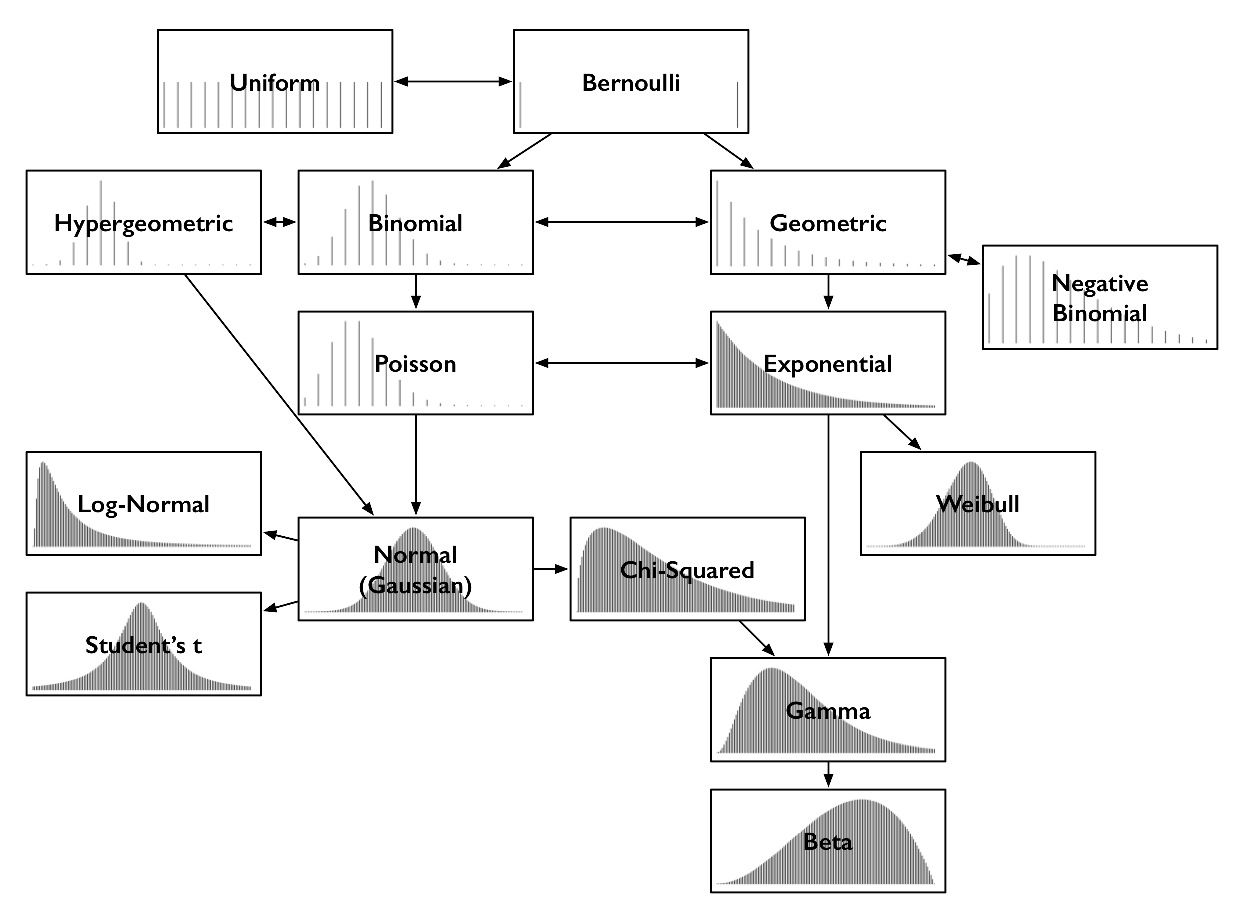
\includegraphics[height=5cm,
    angle=0]{./images/common_distributions.eps}}
\caption{Common distributions}
\label{fig:common_distributions}
\end{figure}


\subsection{Complex distribution: multimodal distributions}
\label{sec:multimodal-distributions}

You might also see complex distributions, such as two peaks that don’t disappear
with different numbers of bins, referred to as a bimodal distribution, or
multiple peaks, referred to as a multimodal distribution,
Fig.\ref{fig:multimodal_distributions}. A multimodal distribution in a sample is
usually an indication that the distribution in the population is not normal.

\begin{figure}[hbt]
  \centerline{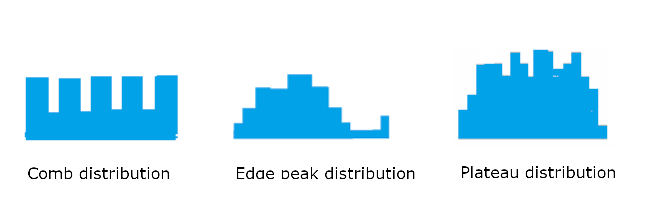
\includegraphics[height=4cm,
    angle=0]{./images/multimodal_distributions.eps}}
\caption{(A) Comb distribution, (B) Edge peak distribution (i.e. a peak at the edge), (C) Plateau distributions}
\label{fig:multimodal_distributions}
\end{figure}

\begin{itemize}
  
  \item  A multimodal distribution is a probability distribution with more than
  one peak, or “mode.” 
  
  
  \item \ldots a bimodal distribution is also multimodal, as there are $>1$ peaks.
  
  {\bf unimodal}: one peak; {\bf bimodal}: two peaks; 
  
  \item \ldots  multimodal distribution is known as a Plateau Distribution when
  there are more than a few peaks close together.
  
  \item A comb distribution is so-called because the distribution looks like a
  comb, with alternating high and low peaks.
  
  NOTE: A comb shape can be caused by rounding off. For example, if you are
  measuring water height to the nearest 10 cm and your class width for the
  histogram is 5 cm, this could cause a comb shape.
  
  \item An edge peak distribution is where there is an additional, out of place
  peak at the edge of the distribution. This usually means that you’ve plotted
  (or collected) your data incorrectly, unless you know for sure your data set
  has an expected set of outliers (i.e. a few extreme views on a survey).
  
  \item You might also see a large spike in density for a given value or small
  range of values indicating outliers, often occurring on the tail of a
  distribution far away from the rest of the density.
  
  
  \item When thinking about the cause of the multimodality, you may want to take
  a close look at your data; what may be going on is that two or more
  distributions are being mapped at the same time. This is opposed to a true
  multimodal distribution, where only one distribution is mapped.
  
\end{itemize}

\subsection{-- preprocess data}
\label{sec:pre-processing-data}

It is possible that the data does match a common probability distribution, but
requires a transformation before parametric density estimation.

For example, you may have outlier values that are far from the mean or center of
mass of the distribution. This may have the effect of giving incorrect estimates
of the distribution parameters and, in turn, causing a poor fit to the data.
These outliers should be removed prior to estimating the distribution
parameters.

Another example is the data may have a skew or be shifted left or right. In this
case, you might need to transform the data prior to estimating the parameters,
such as taking the log or square root, or more generally, using a power
transform like the Box-Cox transform.



\section{Model parameters ($\boldsymbol{\theta}$) estimation}

Suppose we have a collection of samples (i.e. data points) $X$.

The model that we use, i.e. the estimator (Sect.\ref{sec:estimator}) to capture
the properties of the data, has parameters $\boldsymbol{\theta}$.

\section{Coin flipping example}

Example: $X$ - the observatio data - is a sequence of independent coin flips,
then $\boldsymbol{\theta}$ is a single value representing the probability that a
coin comes up heads when flipped.

We want to find the most likely value for the parameters of our model.
We formulate the problem as 
\begin{equation}
\mathop{\mathrm{argmax}} P(\boldsymbol{\theta}\mid X)
\end{equation}

Using Bayes' rule, this is the same thing as
\begin{equation}
\mathop{\mathrm{argmax}} \frac{P(X \mid \boldsymbol{\theta})P(\boldsymbol{\theta})}{P(X)}.
\end{equation}

The expression $P(X)$, a parameter agnostic probability of generating the data,
 does not depend on $\boldsymbol{\theta}$ at all. So, it can be dropped without
 changing the best choice of $\boldsymbol{\theta}$.
 
In this coin-flipping example, we can also posit that we have no prior
assumption on which set of parameters are better than any others, so we may
declare that $P(\boldsymbol{\theta})$ does not depend on theta either! In other
words, the probability it comes up heads could be any value in $[0,1]$ without
any prior belief it is fair or not (often referred to as an *uninformative
prior*).
So, our best choice of $\boldsymbol{\theta}$ is the maximum likelihood estimate
for $\boldsymbol{\theta}$, or choose the value $\hat{\boldsymbol{\theta}}$ so
that once we use the model, we will maximize the likelihood/chance to get the
result same/similar to the observation $X$.

\begin{equation}
\hat{\boldsymbol{\theta}} = \mathop{\mathrm{argmax}} _ {\boldsymbol{\theta}} P(X \mid \boldsymbol{\theta}).
\end{equation}

\subsection{Define $\theta$ and estimate it}
\label{sec:maximum-likelihood}

Suppose that we have a single parameter $\theta$ representing the probability that a coin flip is heads.
Then the probability of getting a tails is $1-\theta$.


If our observed data $X$ is a sequence with $n_H$ heads and $n_T$ tails,
\begin{equation}
P(X \mid \theta) = \theta^{n_H}(1-\theta)^{n_T}.
\end{equation} 

Example: If we flip $13$ coins and get the sequence "HHHTHTTHHHHHT", which has $n_H = 9$ and $n_T = 4$
\begin{equation}
P(X \mid \theta) = \theta^9(1-\theta)^4 
\end{equation}

If we scan values of $\theta$
\begin{lstlisting}
%matplotlib inline
import d2l
from mxnet import autograd, np, npx
npx.set_np()

theta = np.arange(0, 1, 0.001)
p = theta**9 * (1 - theta)**4.

d2l.plot(theta, p, 'theta', 'likelihood')
\end{lstlisting}
, we see that the probability reach the maximum when $\hat{\theta} = 9/13$.

This example is simple as we know the closed form solution. In practice, we have
to estimate them, so having the right strategy to estimate is important, and
deep learning is a good way.


\textcolor{red}{what if we have billions of parameters and data points?}
\begin{enumerate}
  \item  too many data points?
  
  
  \item 
\end{enumerate}

\subsection{What if $\theta$ is a vector}
 
What this maximum likelihood method will give us is a way to get that number
from first principals in a way that will generalize to vastly more complex
situations.

\section{Log-likelihood: Logarithm in probability}
\label{sec:maximum-log-likelihood}

When we multiply probability of multiple data points, first notice that, if we
make the assumption that all the data points are independent (e.g. naive Bayes
classifier - Sect.\ref{sec:naive-Bayes-classifier}), we can no longer
practically consider the likelihood itself as it is a product of many
probabilities.

  Indeed, each probability is in $[0,1]$, say typically of size about $1/2$, and
  the product of $(1/2)^{1000000000}$ is far below machine precision.  We cannot
  work with that directly.
    

However, recall that the logarithm turns products to sums,
\begin{equation}
\log((1/2)^{1000000000}) = 1000000000\cdot\log(1/2) \approx -301029995.6\ldots
\end{equation}

This number fits perfectly within even a single precision $32$-bit float.  Thus, we should consider the *log-likelihood*
\begin{equation}
\log(P(X \mid \boldsymbol{\theta})).
\end{equation}

Since the function $x \mapsto \log(x)$ is increasing, maximizing the likelihood
is the same thing as maximizing the log-likelihood.

\section{Naive Bayes classifier}
\label{sec:naive-Bayes-classifier}

If we want to classify a new data point that we have never seen before we have
to make some assumptions about which data points are similar to each other.
 
The naive Bayes classifier, a popular and remarkably clear algorithm, assumes
all features are independent from each other to simplify the computation.

Example: this model to recognize characters in images, i.e. we assume each pixel
is independent from each other (Sect.\ref{sec:dataset-digits-MNIST}).


\begin{lstlisting}
%matplotlib inline
import d2l
import math
from mxnet import gluon, np, npx
npx.set_np()
d2l.use_svg_display()
\end{lstlisting}

In a classification task, we map an example into a category. 
\begin{itemize}
  \item example is an image which is represented as a single vector of $d=28*28=784$.
  
  
 $\mathbf x\in\mathbb R^d$ the features of the example (which is the transformed image with values in [0,1])
  
  \item category is a label either 0 to 9.
  
  $y\in\mathbb R$ the label. 
  
\end{itemize}

\subsection{The impossible approach}

One natural way to express the classification task is via the probabilistic
question: what is the most likely label given the features (i.e., image pixels)?
\begin{equation}
p(y  \mid  \mathbf{x}) \text{ for } y=0, \ldots,9
\end{equation}

The prediction $\hat{y}$ given by the expression:
\begin{equation}
\hat{y} = \mathrm{argmax} \> p(y  \mid  \mathbf{x}).
\end{equation}

Unfortunately, this requires that we estimate $p(y  \mid  \mathbf{x})$ for every
value of $\mathbf{x} = x_1, ..., x_d$.
If we had $30$ such binary features, that would mean that we need to be prepared
to classify any of $2^{30}$ (over 1 billion!) possible values of the input
vector $\mathbf{x}$.

\subsection{The simpler, yet also impossible approach}

We revert the problem, into a more finite output, i.e. the number of label
($d=10$), rather than using the input (d=30).


$$\hat{y} = \mathrm{argmax}_y \> p(y  \mid  \mathbf{x}) = \mathrm{argmax}_y \> \frac{p( \mathbf{x}  \mid  y) p(y)}{p(\mathbf{x})}.$$

with  $\sum_y p(y  \mid  \mathbf{x}) = 1$.

We just need to focus on  $p( \mathbf{x}  \mid  y)$. 
Using the chain rule of probability, we can express the term $p( \mathbf{x}  \mid  y)$ as

$$p(x_1  \mid y) \cdot p(x_2  \mid  x_1, y) \cdot ... \cdot p( x_d  \mid  x_1, ..., x_{d-1}, y).$$

The problem is smaller, yet  we still must estimate roughly $2^d$ parameters.

\subsection{The possible approach, yet wrong result: assumption of independence}

If we assume that {\it the features are conditionally independent of each other,
given the label}, then suddenly we are in much better shape,

\begin{equation}
\hat{y} = \mathrm{argmax}_y \> \prod_{i=1}^d p(x_i  \mid  y) p(y).
\end{equation}

We can pre-calculate (from training data): 

\begin{itemize}
  
  \item ($d\times n$ matrix):
  If we can estimate $\prod_i p(x_i=1  \mid  y)$ for every
$i$ and $y$, and save its value in $P_{xy}[i, y]$, 

here $P_{xy}$ is a $d \times n$ matrix with $n$ being the number of classes and
$y\in\{1, \ldots, n\}$.

  \item  ($n$-length vector): In addition, we estimate $p(y)$ for every $y$ and save it in $P_y[y]$, 
  
  with $P_y$ a $n$-length vector.
\end{itemize}

Then for any new example $\mathbf x$, we could compute

$$ \hat{y} = \mathrm{argmax}_y \> \prod_{i=1}^d P_{xy}[x_i, y]P_y[y],$$

for any $y$.


The assumption of conditional independence has taken the complexity of our model
from an exponential dependence on the number of features $\mathcal{O}(2^dn)$ to
a linear dependence, which is $\mathcal{O}(dn)$.

The problem now is that we do not know $P_{xy}$ and $P_y$, which are estimated given some training data first.


\subsection{-- Estimate $P_{xy}$}


Since we picked black and white images, $p(x_i  \mid  y)$ denotes the
probability that pixel $i$ is switched on for class $y$. 

Just like before we can go and count the number of times $n_{iy}$ such that an
event occurs and divide it by the total number of occurrences of $y$, i.e.,
$n_y$. 

But there is something slightly troubling: certain pixels may never be
black (e.g., for well cropped images the corner pixels might always be white).

A convenient way for statisticians to deal with this problem is to add pseudo
counts to all occurrences. Hence, rather than $n_{iy}$ we use $n_{iy}+1$ and
instead of $n_y$ we use $n_{y} + 1$.

\begin{lstlisting}
n_x = np.zeros((10, 28, 28))
for y in range(10):
    n_x[y] = np.array(X.asnumpy()[Y.asnumpy() == y].sum(axis=0))
P_xy = (n_x + 1) / (n_y + 1).reshape(10, 1, 1)

d2l.show_images(P_xy, 2, 5);
\end{lstlisting}


\subsection{-- Estimate $P_y$}

Estimating $P_y$ is not too hard. Since we are only dealing with $10$ classes,
we may count the number of occurrences $n_y$ for each of the digits and divide
it by the total amount of data $n$.

For instance, if digit 8 occurs $n_8 = 5,800$ times and we have a total of 
$n = 60,000$ images, the probability estimate is $p(y=8) = 0.0967$.


\begin{lstlisting}
X, Y = mnist_train[:]  # All training examples

n_y = np.zeros((10))
for y in range(10):
    n_y[y] = (Y == y).sum()
P_y = n_y / n_y.sum()
P_y
\end{lstlisting}

\subsection{-- Laplace smoothing}

Suppose that we did not use Laplace smoothing when estimating probabilities and
a data point arrived at testing time which contained a value never observed in
training. What would the model output?

Since we picked black and white images, $p(x_i  \mid  y)$ denotes the
probability that pixel $i$ is switched on for class $y$. Just like before we can
go and count the number of times $n_{iy}$ such that an event occurs and divide
it by the total number of occurrences of $y$, i.e., $n_y$.

There are pixels, e.g. certain pixels may never be black (e.g., for well cropped
images the corner pixels might always be white), so the probability is always
zero.

A convenient way for statisticians to deal with this problem is to add pseudo
counts to all occurrences i.e. having an additional image for that label in that
the pixel for that position is black. Hence, rather than $n_{iy}$ we use
$n_{iy}+1$ and instead of $n_y$ we use $n_{y} + 1$. This is also called *Laplace
Smoothing*. It may seem ad-hoc, however it may be well motivated from a Bayesian
point-of-view.







\subsection{-- Test the (failed) naive Bayes classifier}

Given $\mathbf x$, the following functions computes $p(\mathbf x \mid y)p(y)$ for every $y$.

\begin{lstlisting}
def bayes_pred(x):
    x = np.expand_dims(x, axis=0)  # (28, 28) -> (1, 28, 28)
    p_xy = P_xy * x + (1 - P_xy)*(1 - x)
    p_xy = p_xy.reshape(10, -1).prod(axis=1)  # p(x|y)
    return np.array(p_xy) * P_y

image, label = mnist_test[0]
bayes_pred(image)
\end{lstlisting}


\textcolor{red}{IT DOESN''T WORK}: The reason is that the probability, they are
typically numbers between $0.001$ and $1$. We are multiplying $784$ of them.
What happens is that we experience *numerical underflow*, i.e., multiplying all
the small numbers leads to something even smaller until it is rounded down to
zero.

\subsection{The possible approach, and correct result: assumption of independence}


\begin{equation}
 \hat{y} = \mathrm{argmax}_y \> \sum_{i=1}^d \log P_{xy}[x_i, y] + \log P_y[y].
\end{equation}

\begin{lstlisting}
log_P_xy = np.log(P_xy)
log_P_xy_neg = np.log(1 - P_xy)
log_P_y = np.log(P_y)

def bayes_pred_stable(x):
    x = np.expand_dims(x, axis=0)  # (28, 28) -> (1, 28, 28)
    p_xy = log_P_xy * x + log_P_xy_neg * (1 - x)
    p_xy = p_xy.reshape(10, -1).sum(axis=1)  # p(x|y)
    return p_xy + log_P_y

py = bayes_pred_stable(image)
py


# Convert label which is a scalar tensor of int32 dtype
# to a Python scalar integer for comparison
py.argmax(axis=0) == int(label)
\end{lstlisting}
 
\subsection{-- Test the naive Bayes classifier}

\begin{lstlisting}
def predict(X):
    return [bayes_pred_stable(x).argmax(axis=0).astype(np.int32) for x in X]

X, y = mnist_test[:18]
preds = predict(X)
d2l.show_images(X, 2, 9, titles=[str(d) for d in preds]);
\end{lstlisting}

The overall accuracy
\begin{lstlisting}
X, y = mnist_test[:]
preds = np.array(predict(X), dtype=np.int32)
float((preds == y).sum()) / len(y)  # Validation accuracy
\end{lstlisting}


The relatively poor performance is due to the incorrect statistical assumptions
that we made in our model: we assumed that each and every pixel are
independently generated, depending only on the label. This is clearly not how
humans write digits, and this wrong assumption led to the downfall of our overly
naive (Bayes) classifier.

REMEMBER: Modern deep networks achieve error rates of less than 0.01.



\section{Negative log-likelihood: maximum-likelihood in Deep Learning}



\subsection{negative choice: minimizing rather than mazimizing}

In Deep Learning, the last layer's output is often in the form of probability,
or likelihood.
From that, we often work with loss functions, where we wish to minimize the
loss.
We may turn maximum likelihood into the minimization of a loss by taking
$-\log(P(X \mid \boldsymbol{\theta}))$, which is the {\bf negative log-likelihood}.

Consider the coin flipping problem from before, maximizing the log-likehood is
turned into a problem of minimizing the loss function, by changing the $\theta$
parameters in steepest gradient descent.
 
$$
-\log(P(X \mid \boldsymbol{\theta})) = -\log(\theta^{n_H}(1-\theta)^{n_T}) = -(n_H\log(\theta) + n_T\log(1-\theta)).
$$

Example: here, we iterate over 10 times, but it can be more to converge
\begin{lstlisting}{lang="python"}
# Set up our data
n_H = 8675309
n_T = 25624

# Initialize our paramteres
theta = np.array(0.5)
theta.attach_grad()

# Perform gradient descent
lr = 0.00000000001
for iter in range(10):
    with autograd.record():
        loss = -(n_H * np.log(theta) + n_T * np.log(1 - theta))
    loss.backward()
    theta -= lr * theta.grad

# Check output
theta, n_H / (n_H + n_T)
\end{lstlisting}

\subsection{log- choice: simple form}

Due to independence assumptions, most probabilities we encounter in machine
learning are products of individual probabilities, which makes the use of
 log-likelihood even more important.
It turns from product calculation

$$
P(X\mid\boldsymbol{\theta}) = p(x_1\mid\boldsymbol{\theta})\cdot p(x_2\mid\boldsymbol{\theta})\cdots p(x_n\mid\boldsymbol{\theta}).
$$
which makes the calculation of derivatives too hard
$$
\begin{aligned}
\frac{\partial}{\partial \boldsymbol{\theta}} P(X\mid\boldsymbol{\theta}) & = \left(\frac{\partial}{\partial \boldsymbol{\theta}}P(x_1\mid\boldsymbol{\theta})\right)\cdot P(x_2\mid\boldsymbol{\theta})\cdots P(x_n\mid\boldsymbol{\theta}) \\
& \quad + P(x_1\mid\boldsymbol{\theta})\cdot \left(\frac{\partial}{\partial \boldsymbol{\theta}}P(x_2\mid\boldsymbol{\theta})\right)\cdots P(x_n\mid\boldsymbol{\theta}) \\
& \quad \quad \quad \quad \quad \quad \quad \quad \quad \quad \vdots \\
& \quad + P(x_1\mid\boldsymbol{\theta})\cdot P(x_2\mid\boldsymbol{\theta}) \cdots \left(\frac{\partial}{\partial \boldsymbol{\theta}}P(x_n\mid\boldsymbol{\theta})\right).
\end{aligned}
$$

to a simpler form
$$
-\log\left(P(X\mid\boldsymbol{\theta})\right) = -\log(P(x_1\mid\boldsymbol{\theta})) - \log(P(x_2\mid\boldsymbol{\theta})) \cdots - \log(P(x_n\mid\boldsymbol{\theta})),
$$
which make the calculation of derivatives easier (This requires only $n$ divides and $n-1$ sums, and thus is linear time in the inputs.)
 
$$
- \frac{\partial}{\partial \boldsymbol{\theta}} \log\left(P(X\mid\boldsymbol{\theta})\right) = \frac{1}{P(x_1\mid\boldsymbol{\theta})}\left(\frac{\partial}{\partial \boldsymbol{\theta}}P(x_1\mid\boldsymbol{\theta})\right) + \cdots + \frac{1}{P(x_n\mid\boldsymbol{\theta})}\left(\frac{\partial}{\partial \boldsymbol{\theta}}P(x_n\mid\boldsymbol{\theta})\right).
$$

\subsection{cross-entropy: has relationship to information theory}

The third and final reason to consider the negative log-likelihood is the relationship to information theory.
Information theory tells whether the model is generalized enough, i.e. whether it can encode enough information.
This is a rigorous mathematical theory which gives a way to measure the degree of information or randomness in a random variable.


The key object of study in that field is the entropy which is 

$$
H(p) = -\sum_{i} p_i \log_2(p_i),
$$

which measures the randomness of a source

If we take our negative log-likelihood and divide by the number of data points,
we get a relative of entropy known as cross-entropy.


This theoretical interpretation alone would be sufficiently compelling to
motivate reporting the average negative log-likelihood over the dataset as a way
of measuring model performance.

\chapter{Information Theory: Maths od Deep Learning}

Information comes in different format, e.g. music, written language, spoken
language, video, \ldots

Information provides a common language across disciplinary rifts: from
Shakespeare’s Sonnet to researchers’ paper on Cornell ArXiv, from Van Gogh’s
printing Starry Night to Beethoven’s music Symphony No. 5, from the first
programming language Plankalkül to the state-of-the-art machine learning
algorithms. 

\textcolor{red}{Everything must follow the rules of information theory, no matter the format.}
With information theory, we can measure and compare how much information is
present in different signals.

\section{Information: the soul}

Let’s start with the “soul” of information theory: information. Information can
be encoded in anything with a particular sequence of one or more encoding
formats.

Suppose that we task ourselves with trying to define a notion of information.
What could be are starting point?

\subsection{Example: draw a card from a deck}

Consider the following thought experiment. We have a friend with a deck of
cards. They will shuffle the deck, flip over some cards, and tell us statements
about the cards. We will try to assess the information content of each
statement.

\subsection{-- statement: I see a card}


First, they flip over a card and tell us, “I see a card.” 

Does that statement provides us any new information? 

NO: as we know for sure it is a card. 

So, the information of that statement is zero. 


\subsection{-- statement: I see a heart}

Next, they flip over a card and say, “I see a heart.” 

This provides us some information, but in reality there are only 4 different
suits that were possible, each equally likely, so we are not surprised by this
outcome. Before this statement, we can guess, with probability $1/4$, that it's a heart.

The statement brings some information, but the information is low. 

\subsection{-- statement: I see a 3 of spades}


Next, they flip over a card and say, “This is the 3 of spades.” This is more
information. Indeed there were 52 equally likely possible outcomes, and our
friend told us which one it was. Before this statement, we can guess, with
probability $1/52$, that it's a 3 of spades.

So, the statement provides a medium amount of information.

\subsection{-- statement: tell the exact order of 52 cards}


Suppose that finally they flip over every card from the deck and read off the
entire sequence of the shuffled deck. There are 52! different orders to the
deck, again all equally likely. Before this statement, the chance to tell correctly is extremely small.


So we need a lot of information to know which one it is.

\subsection{Information level = degree of surprise}

As a starting point, rather than caring about the knowledge, we may build off
the idea that information represents the degree of surprise or the abstract
possibility of the event.

For example, if we want to describe an unusual event, we need a lot information.
For a common event, we may not need much information.

\section{Information level of a single discrete event: Shannon's work (self-information)}
\label{sec:self-information}

In 1948, Claude E. Shannon published A Mathematical Theory of Communication
(Shannon.1948) establishing the theory of information. In his book, Shannon
introduced the concept of information entropy for the first time. We will begin
our journey here.

The information level is quantified in the form of {\bf number of bits required}.
Shannon introduced the terminology bit as the unit of information, which was
originally created by John Tukey. 

\textcolor{red}{What is a 'bit'?}.  Historically, an antique transmitter can
only send or receive two types of code:
0 and 1. Coincidently, binary encoding is still in common use on all modern
digital computers. Hence, a series of binary digits of length $n$ contains $n$
bits of information.

Consider a series contains $n$ bits of information: Now, suppose that for any
series of codes, each $0$ or $1$ occurs with a probability of $\frac{1}{2}$.
Hence, an event $X$ with a series of codes of length $n$, occurs with a
probability of $\frac{1}{2^n}$.

The probability $p$ (for an event to occur) is transferred to the concept of
number of bits. Shannon gave the answer by defining {\bf self-information}

$$I(X) = - \log_2 (p),$$

as the *bits* of information we have received for this event $X$.
Note that we will always use base-2 logarithms here.
So, for the sake of simplicity, the rest of this section will omit the subscript 2
in the logarithm notation, i.e., $\log(.)$ always refers to $\log_2(.)$.

\begin{lstlisting}
from mxnet import np
from mxnet.metric import NegativeLogLikelihood
from mxnet.ndarray import nansum
import random

def self_information(p):
    return -np.log2(p)

self_information(1/64)
\end{lstlisting}

\section{(Shannon) Entropy: information level in single random variable}

In 1948, Claude E. Shannon published A Mathematical Theory of Communication
(Shannon.1948) establishing the theory of information. In his book, Shannon
introduced the concept of information entropy for the first time. 
In Sect.\ref{sec:self-information}, we talked about {\bf self-information}.

As self-information only measures the information of a single discrete event, we
need a more generalized measure for any random variable of either discrete or
continuous distribution.

\subsection{Axioms of Shannon Entropy}
\label{sec:Shannon-entropy}

To be able to quantify Shannon entropy of a random variable, we rely on the
following axioms, aka {\it axioms of Shannon Entropy}.
It will turn out that the following collection of common-sense statements force
us to a unique definition of information (Csiszar.2008).

There are 3 important axioms
\begin{enumerate}
\item The information gained when observing (nearly) certain events is (nearly) zero.

\item  The information gained by observing a random variable does not depend on what
  we call the elements, or the presence of additional elements which have
  probability zero.

\item The information gained when observing two random variables is no more than
the sum of the information we gain by observing them separately. 

If they are independent, then it is exactly the sum.

\end{enumerate}

While proving this fact is beyond the scope of our text, it is important to know
that this uniquely determines the form that entropy must take. The only
ambiguity that these allow is in the choice of fundamental units, which is most
often normalized.


For any random variable $X$ that follows a probability distribution $P$ with a
probability density function (p.d.f.) or a probability mass function (p.m.f.)
$p(x)$, we measure the expected amount of information through *entropy* (or
*Shannon entropy*)

$$H(X) = - E_{x \sim P} [\log p(x)].$$

why do we use an expectation of a negative logarithm? Here are some intuitions.
\begin{enumerate}
  \item Logarithm is important as it converts multiply to sum operator.
  
  Suppose that $p(x) = f_1(x) f_2(x) \ldots, f_n(x)$, where each component
  function $f_i(x)$ is independent from each other. This means that each
  $f_i(x)$ contributes independently to the total information obtained from
  $p(x)$.
  
  We want the entropy formula to be additive over independent random variables.
  Luckily, $\log$ can naturally turn a product of probability distributions to a
  summation of the individual terms.
  
  \item Why negative Log? 
  
  Intuitively, more frequent events should contain less information than less
  common events, since we often gain more information from an unusual case than
  from an ordinary one. So, events with smaller probability should has larger
  entropy than events with larger probability.
  
  However, $\log$ is monotonically increasing with the probabilities, and indeed
  negative for all values in $[0, 1]$.
  So, we need to construct a monotonically decreasing relationship between the
  probability of events and their entropy, which will ideally be always
  positive, we add a negative sign in front of $\log$ function.
  
  \item Why Expectation function?
  
   Consider a random variable $X$. We can interpret the self-information
   ($-\log(p)$) as the amount of *surprise* we have at seeing a particular
   outcome. Indeed, as the probability approaches zero, the surprise becomes
   infinite (i.e. very very large).
   
   Similarly, we can interpret The entropy as the average amount of surprise
   from observing $X$.
   
   For example, imagine that a slot machine system emits statistical
   independently symbols ${s_1, \ldots, s_k}$ with probabilities ${p_1, \ldots,
   p_k}$ respectively. Then the entropy of this system equals to the average
   self-information from observing each output, i.e.,
   
   $$H(S) = \sum_i {p_i \cdot I(s_i)} = - \sum_i {p_i \cdot \log p_i}.$$
   
   
\end{enumerate}


\subsection{Shannon Entropy of a discrete random variable}

To be specific, if $X$ is discrete, $$H(X) = - \sum_i p_i \log p_i \text{, where } p_i = P(X_i).$$ 


Python code: MXNet library
\begin{lstlisting}
def entropy(p):
    entropy = - p * np.log2(p)
    # nansum will sum up the non-nan number
    out = nansum(entropy.as_nd_ndarray())
    return out

entropy(np.array([0.1, 0.5, 0.1, 0.3]))
\end{lstlisting}

\subsection{Shannon Entropy of a continuous random variable}

Otherwise, if $X$ is continuous, we also refer entropy as *differential entropy* 

$$H(X) = - \int_x p(x) \log p(x) \; dx.$$

We can estimate by generating many discrete values of $X$, with tiny gap between them.

\subsection{Logarithm is important to use}


For any random variable $X$ that follows a probability distribution $P$ with a
probability density function (p.d.f.) or a probability mass function (p.m.f.)
$p(x)$, we measure the expected amount of information through {\bf entropy} (or
{\bf Shannon entropy}) - Sect.\ref{sec:Shannon-entropy}.

Suppose that $p(x) = f_1(x) f_2(x) \ldots, f_n(x)$, where each component
function $f_i(x)$ is independent from each other. This means that each $f_i(x)$
contributes independently to the total information obtained from $p(x)$. As
discussed above, we want the entropy formula to be additive over independent
random variables. Luckily, $\log$ can naturally turn a product of probability
distributions to a summation of the individual terms.


\subsection{Summary of entropy}

Here, we refer to X as an event and P as the probability distribution of X.

\begin{enumerate}
  \item  * Entropy is non-negative, i.e., $H(X) \geq 0, \forall X$.

  \item * If $X \sim P$ with a p.d.f. or a p.m.f. $p(x)$, and we try to estimate
  $P$ by a new probability distribution $Q$ with a p.d.f. or a p.m.f. $q(x)$,
  then 
  
  $$H(X) = - E_{x \sim P} [\log p(x)] \leq  - E_{x \sim P} [\log q(x)], \text{ with equality if and only if } P = Q.$$  
  
  Alternatively, $H(X)$ gives a
  lower bound of the average number of bits needed to encode symbols drawn from
  $P$.
  
  \item * If $X \sim P$, then $x$ conveys the maximum amount of information if
  it spreads evenly among all possible outcomes. Specifically, if the
  probability distribution $P$ is discrete with $k$-class 
  $\{p_1, \ldots, p_k \}$, then 
  
  $$H(X) \leq \log(k), \text{ with equality if and only if } p_i =
  \frac{1}{k}, \forall x_i.$$ 
  
  If $P$ is a continuous random variable, then the
  story becomes much more complicated.  However, if we additionally impose that
  $P$ is supported on a finite interval (with all values between $0$ and $1$),
  then $P$ has the highest entropy if it is the uniform distribution on that
  interval.
  
  
\end{enumerate}


\section{(Shannon) Entropy: mutual information (between two  random variables)}

How about the entropy of a pair random variables $(X, Y)$?  We can think of
these techniques as trying to answer the following type of question, "What
information is contained in $X$ and $Y$ together compared to each separately? 
Is there redundant information, or is it all unique?"


For the following discussion, we always use $(X, Y)$ as a pair of random
variables that follows a joint probability distribution $P$ with a p.d.f. or a
p.m.f. $p_{X, Y}(x, y)$, while $X$ and $Y$ follow probability distribution
$p_X(x)$ and $p_Y(y)$, respectively.


$$H(X, Y) = -E_{(x, y) \sim P} [\log p_{X, Y}(x, y)]. $$

We can think of $H(X,Y)$ as telling us the total randomness in the pair of
random variables.  As a pair of extremes, if $X = Y$ are two identical random
variables, then the information in the pair is exactly the information in one
and we have $H(X, Y) = H(X) = H(Y)$.

On the other extreme, if $X$ and $Y$ are independent then $H(X, Y) = H(X) + H(Y)$.  

So, we have this inequality
$$
H(X), H(Y) \le H(X, Y) \le H(X) + H(Y).
$$

\subsection{pair of discrete random variables}


$$H(X, Y) = - \sum_{x} \sum_{y} p_{X, Y}(x, y) \log p_{X, Y}(x, y).$$

\subsection{pair of continuous random variables}

we define the *differential joint entropy* as 

$$H(X, Y) = - \int_{x, y} p_{X, Y}(x, y) \ \log p_{X, Y}(x, y) \;dx \;dy.$$



\begin{lstlisting}
def joint_entropy(p_xy):
    joint_ent = -p_xy * np.log2(p_xy)
    # nansum will sum up the non-nan number
    out = nansum(joint_ent.as_nd_ndarray())
    return out

joint_entropy(np.array([[0.1, 0.5], [0.1, 0.3]]))
\end{lstlisting}
This is the same *code* as before, but now we interpret it differently as working on the joint distribution of the two random variables.




\section{(Mutual) Information in Deep Learning}

Machine learning aims to extract interesting signals from data and make critical
predictions.

Information theory studies encoding, decoding, transmitting, and manipulating
information. As a result, information theory provides fundamental language for
discussing the information processing in machine learned systems.

NOTE:  many machine learning applications use the cross entropy loss.
This loss can be directly derived from information theoretic considerations.


In natural language processing, one of the most difficult problems is the
ambiguity resolution, or the issue of the meaning of a word being unclear from
context. For example, recently a headline in the news reported that “Amazon is
on fire”. You may wonder whether the company Amazon has a building on fire, or
the Amazon rain forest is on fire.

In this case, mutual information can help us resolve this ambiguity. We first
find the group of words that each has a relatively large mutual information with
the company Amazon, such as e-commerce, technology, and online. Second, we find
another group of words that each has a relatively large mutual information with
the Amazon rain forest, such as rain, forest, and tropical.


When we need to disambiguate “Amazon”, we can compare which group has more
occurrence in the context of the word Amazon. In this case the article would go
on to describe the forest, and make the context clear.






\chapter{Stats: Maths of Deep Learning}

Using a proper stastistics technique, we will know whether  when improvements
are significant, or only the result of random fluctuations in the training
process.

\begin{itemize}
  \item  The earliest reference of statistics can be traced back to an Arab scholar Al-Kindi in the $9^{\mathrm{th}}$-century
  
  He gave a detailed description of how to use statistics and frequency analysis to decipher encrypted messages
  
  \item the modern statistics arose from Germany in 1700s (after 800 years), when the researchers
  focused on the demographic and economic data collection and analysis
  
  \item Today, statistics is the science subject that concerns the collection,
  processing, analysis, interpretation and visualization of data.
\end{itemize}



\section{Descriptive vs Statistical (inference)}
\label{sec:statistical-inference}
\label{sec:descriptive-inference}

More specifically, statistics can be divided to descriptive statistics and statistical inference
\begin{enumerate}
  \item {\bf descriptive statistics}:
  summarizing and illustrating the features of a collection of observed data, which is referred to as a sample.
  
  The sample is drawn from a population, denotes the total set of similar individuals, items, or events of our experiment interests. 
  
  \item {\bf statistical inference}:
   deduces the characteristics of a population from the given samples, based on
   the assumptions that the sample distribution can replicate the population
   distribution at some degree.
   
   This often requires the choice of an estimator (Sect.\ref{sec:estimator}), and through this estimator, we conduct a {\bf hypothesis testing} (Sect.\ref{sec:hypothesis-testing})
   
\end{enumerate}

\section{Estimator}
\label{sec:estimator}

In statistics, an {\bf estimator} is {\it a function of given samples} and is
used to estimate the true parameter $\theta$. This is aka the {\bf choice of a
model} representing a truth unknown problem.

We will write $\hat{\theta}_n = \hat{f}(x_1, \ldots, x_n)$ for the estimate of
$\theta$ after observing the samples
\begin{equation}
{ x_1, x_2, \ldots, x_n }
\end{equation}.

Example:
\begin{enumerate}
  \item $\theta$ is the parameter in a Bernoulli: 
  
  If you have a number of samples from a Bernoulli random variable, then {\it the
  maximum likelihood estimate for the probability the random variable} is one can
  be obtained by {\it counting the number of ones observed and dividing by the total
  number of samples.}
  
  \item $\theta$ is the mean of a Gaussian:
  
  the maximum likelihood estimate of the mean of a Gaussian given a number of
  samples is given by the average value of all the samples.
  
  \item 
\end{enumerate}

These estimators will almost never give the true value of the parameter, but
ideally for a large number of samples the estimate will be close.
This is known as the {\bf law of large numbers}.

Example: \verb!xs! is a Gaussian random variable with mean zero and variance one.
Then we construct \verb!ys! the density 
\begin{lstlisting}{lang="python"}
import d2l
from mxnet import np, npx
import random
npx.set_np()

# Sample datapoints and create y coordinate
epsilon = 0.1
random.seed(8675309)
xs = np.random.normal(loc=0, scale=1, size=(300,))

ys = [np.sum(np.exp(-(xs[0:i] - xs[i])**2 / (2 * epsilon**2))
             / np.sqrt(2*np.pi*epsilon**2)) / len(xs) for i in range(len(xs))]

# Compute true density
xd = np.arange(np.min(xs), np.max(xs), 0.01)
yd = np.exp(-xd**2/2) / np.sqrt(2 * np.pi)

# Plot the results
d2l.plot(xd, yd, 'x', 'density')
d2l.plt.scatter(xs, ys)
d2l.plt.axvline(x=0)
d2l.plt.axvline(x=np.mean(xs), linestyle='--', color='purple')
d2l.plt.title("Sample Mean: {:.2f}".format(float(np.mean(xs))))
d2l.plt.show()
\end{lstlisting}

To see how closed the estimation of the estimator to the truth yet unknown parameter, we can use one of the 3 methods:
\begin{enumerate}
  \item  the mean squared error (L2 loss), 
  
  \item the standard deviation, and 
  
  \item statistical bias.
\end{enumerate}

\subsection{Mean squared error (L2 loss)}
\label{sec:loss-L2-loss}
\label{sec:mean-squared-error}

MSE is always non-negative.
As a measure to evaluate an estimator, the closer its value to zero, the closer
the estimator is close to the true parameter $\theta$.

\begin{equation}
\mathrm{MSE} (\hat{\theta}_n, \theta) = E[(\hat{\theta}_n - \theta)^2].
\end{equation}

NOTE: It is the most commonly used regression loss function. 

Even though MSE is a natural metric, its value can be large due to 2 sources of errors:
\begin{enumerate}
  \item The fluctuation in the estimator due to randomness in the dataset: which is explained by the 
  variance (Sect.\ref{sec:math-variance}), and
  
  The high variance usually results from a too complex model, which overfits the
  training data.
  As a result, an overfitting model is sensitive to small fluctuations in the
  data. If a model suffers from high variance, we often say it is overfitting
  and lack of flexibility
  
  \item systematic error in the estimator due to the estimation procedure: which
  is explained by the statistical bias (Sect.\ref{sec:math-statistical-bias})
  
  The bias error is commonly seen in choosing a wrong model, e.g. a simple model
  (such as a linear regression model), which cannot extract high dimensional
  relations between the features and the outputs.
  
  If a model suffers from high bias error, we often say it is underfitting or
  lack of generalization.
  
\end{enumerate}

The mean squared error can be divided into precisely two sources of error, see below: the
error from high bias and the error from high variance. 
\begin{equation}
\begin{aligned}
\mathrm{MSE} (\hat{\theta}_n, \theta) &= E[(\hat{\theta}_n - E(\hat{\theta}_n) + E(\hat{\theta}_n) - \theta)^2] \\
 &= E[(\hat{\theta}_n - E(\hat{\theta}_n))^2] + E[(E(\hat{\theta}_n) - \theta)^2] \\
 &= \mathrm{Var} (\hat{\theta}_n) + [\mathrm{bias} (\hat{\theta}_n)]^2.\\
\end{aligned}
\end{equation}

In Python
\begin{lstlisting}{lang="python"}
# Mean squared error
def mse(data, true_theta):
    return(np.mean(np.square(data - true_theta)))
\end{lstlisting}

Example: the truth $\theta$ is the mean in a normal distribution $\mathcal{N}(\theta, \sigma^2)$ 
\begin{lstlisting}
theta_true = 1
sigma = 4
\end{lstlisting}
Now, what we really have is a collection of samples
\begin{lstlisting}
sample_length = 10000
samples = np.random.normal(theta_true, sigma, sample_length)
\end{lstlisting}
Using the samples, we want to estimate the real theta by using the estimator as the mean of the samples
\begin{lstlisting}
theta_est = np.mean(samples)
theta_est
\end{lstlisting}
We ask, what is the error of this choice of the estimator?
\begin{lstlisting}{lang="python"}
mse(samples, theta_true)
\end{lstlisting}
the returned value is the same as 
\begin{lstlisting}
bias = stat_bias(theta_true, theta_est)
np.square(samples.std()) + np.square(bias)
\end{lstlisting}

\subsection{Statistical bias}
\label{sec:math-statistical-bias}
Statistical bias tells whether there is a systematic error, i.e. the estimation
procedure is accurate or not
\begin{equation}
\mathrm{bias}(\hat{\theta}_n) = E(\hat{\theta}_n - \theta) = E(\hat{\theta}_n) - \theta
\end{equation}

when $\mathrm{bias}(\hat{\theta}_n) = 0$, the expectation of the estimator
$\hat{\theta}_n$ is equal to the true value of parameter.
In this case, we say $\hat{\theta}_n$ is an unbiased estimator.  

In general, an unbiased estimator is better than a biased estimator since its
expectation is the same as the true parameter.

For example: in order to estimate the mean of a population, based on its $n$ samples, the biased estimator is 
\begin{equation}
\hat{x} = \frac{1}{n} \sum x_i
\end{equation}
, while the unbiased estimator is
\begin{equation}
\hat{x} = \frac{1}{n-1} \sum x_i
\end{equation}


\begin{mdframed}

It is worth being aware, however, that biased estimators are frequently used in
practice.  There are cases where unbiased estimators do not exist without
further assumptions, or are intractable to compute.

This may seem like a significant flaw in an estimator, however the majority of
estimators encountered in practice are at least asymptotically unbiased in the
sense that the bias tends to zero as the number of available samples tends to
infinity:
$$\lim_{n \rightarrow \infty} \mathrm{bias}(\hat{\theta}_n) = 0$$ 
\end{mdframed}

In Python
\begin{lstlisting}{lang="python"}
# Statistical bias
def stat_bias(true_theta, est_theta):
    return(np.mean(est_theta) - true_theta)
\end{lstlisting}

\subsection{Variance + Standard deviation}
\label{sec:math-variance}

*standard deviation* (or *standard error*) is defined as the squared root of the
variance. It is used to measure the randomness in the estimator. Instead of
comparing to the true population value $\theta$, we compare to the expected
sample mean $E(\hat{\theta}_n)$.
Thus we are not measuring how far the estimator tends to be from the true value,
but instead we measuring the fluctuation of the estimator itself.
 
 
We may measure the degree of fluctuation of an estimator by measuring the
standard deviation or variance of that estimator.

\begin{equation}
\sigma_{\hat{\theta}_n} = \sqrt{\mathrm{Var} (\hat{\theta}_n )} = \sqrt{E[(\hat{\theta}_n - E(\hat{\theta}_n))^2]}.
\end{equation}


\begin{itemize} 
  \item Python:  in MXNet library, we get the standard deviation  is by simply calling a.std() for a ndarray “a”, 
\end{itemize}


\section{Hypothesis testing (One-sample)}
\label{sec:hypothesis-testing}

{\bf Hypothesis testing} is the most common topics in {\bf statistical
inference} (Sect.\ref{sec:statistical-inference}), which is the field trying to
deduce the characteristics of a population from the given samples, based on
the assumptions that the sample distribution can replicate the population
distribution at some degree.
   
Via the samples, first we assume the choice of an  estimator
(Sect.\ref{sec:estimator}), and through this estimator, we conduct a {\bf
hypothesis testing}.

\begin{mdframed}
 
While hypothesis testing was popularized in the early 20th century, the first
use can be traced back to John Arbuthnot in the 1700s. John tracked 80-year
birth records in London and concluded that more men were born than women each
year.

Following that, the modern significance testing is the intelligence heritage by
Karl Pearson who invented $p$-value and Pearson’s chi-squared test
$\chi$-squared test).

William Gosset who is the father of Student’s t-distribution, and Ronald Fisher
who initialed the null hypothesis and the significance test.
\end{mdframed}

A hypothesis test is a way of  {\it evaluating some evidence (i.e. the observed
data) against the default statement about a population.} - the default statement
is called a {\bf NULL hypothesis} $H_o$ which we try to reject using the
observed data. A null hypothesis is often stated in a declarative form which
posits a relationship between variables. It should reflect the brief as explicit
as possible, and be testable by statistics theory.


The {\bf *alternative hypothesis} $H_A$ (or $H_1$) is a statement that is
contrary to the null hypothesis.

Example:
Imagine you are a chemist. After spending thousands of hours in the lab, you
develop a new medicine which can dramatically improve one's ability to
understand math. To show its magic power, you need to test it. Naturally, you
may need some volunteers to take the medicine and see whether it can help them
learn math better. How do you get started?
\begin{enumerate}
  \item  Sample selections
  
  \item 
\end{enumerate}

\section{Matplotlib package}

\begin{lstlisting}
import matplotlib.pyplot as plt
\end{lstlisting}

\section{Seaborn package (data visualization)}
\label{sec:seaborn}

Seaborn is complimentary to Matplotlib and it specifically targets statistical
data visualization. But it goes even further than that
 
``If matplotlib 'tries to make easy things easy and hard things possible',
seaborn tries to make a well-defined set of hard things easy too." 
One of these hard things or frustrations had to do with the default Matplotlib
parameters.

\begin{lstlisting}
import seaborn as sns

# Plot parameters
sns.set()
%pylab inline
pylab.rcParams['figure.figsize'] = (4, 4)
plt.rcParams['xtick.major.size'] = 0
plt.rcParams['ytick.major.size'] = 0
\end{lstlisting}
\url{https://seaborn.pydata.org/}

\url{https://elitedatascience.com/python-seaborn-tutorial}

\chapter{Regression + Classification (Machine Learning)}

\section{Choice of a model}

A model is a mathematical representation of a real world domain/problem, hoping
that the model capture the properties/behaviors of the real-world problem. 
\begin{itemize}
  \item {\bf as in linear regression}: 
  \begin{enumerate}
    \item  uni-variate, e.g. the relationship between the price of oil and the price of clothes 
  
    \item multi-variate, e.g. the relationship between the price of oil (y) and the price of clothes (x1) and the weather (x2).
  \end{enumerate}
  
  \item {\bf as in non-linear regression}
  
  \item {\bf as in classiciation} (Machine Learning: SVM, DeepLearning): y = f(x)
  
  given the input $x$, it should tell the label $y$ of that sample.
  
\end{itemize}

The choice of a model is known as an {\bf estimator} (Sect.\ref{sec:estimator}),
and thus there are errors that come with such choice
(Sect.\ref{sec:loss-L2-loss}). The quality of a model 
\begin{enumerate}
  \item high {\bf bias} error: it means the choice of model is too simple, and thus cannot capture the more-complicated relationship 
  
  \item high {\bf variance} error: it means the learned model is overfitting the samples data, and thus is sensitive to small fluctuation in the samples
  
\end{enumerate}

\chapter{Distribution: Maths of Deep Learning}

\begin{enumerate}
  \item  Bernoulli random variables can be used to model events with a yes/no outcome.
  \item  Discrete uniform distributions model selects from a finite set of possibilities.
  \item  Continuous uniform distributions select from an interval.
  \item  Binomial distributions model a series of Bernoulli random variables, and count the number of successes.
  \item  Poisson random variables model the arrival of rare events.
  \item  Gaussian random variables model the result of adding a large number of independent random variables together.
\end{enumerate}


\section{Bayesian: importance sampling with SIR algorithm (1987, 1988)}

Suppose you have some knowledge (i.e. assumption) about distribution of
parameters/inputs, i.e. pre-model distribution.
Of course, you can draw samples from this pre-model distribution. 

Consider reading Sect.\ref{sec:probability-density-estimation}.

You know run these samples to the (deterministic/mechanistic) model, you get the quality of the output. So, the quality of the output gives you
the information about the validity of the input, i..e. the imporantce.

To get the right distribution of the input, once we incorporate the knowledge from the model, we can apply 
{\bf sampling-importance-resampling} algorithm (Rubin 1987, 1988).

\begin{itemize}
  \item  draw large samples of size $k$ of inputs $\theta$ from $p^{[\theta]}(\theta)$
  
  \item  test the importance of the sample: so that we can assign a (importance
  sampling) weight $w_i$ to each input sample $\theta_i$
  
  \item {\bf resampling}: draw a second sample of size $l$ from discrete distribution with value $\theta_i$ and associated probabilities $w_i$.
\end{itemize}

The second sample is approximately a sample from the postmodel distribution and it is the
basis for inference about inputs outputs and quantities of interest in the Bayesian synthesis method


\chapter{Linear NN: }

Before we get into the details of deep neural networks, we need to cover the basics of neural network training.
The entire training process
\begin{enumerate}
  \item collect samples correctly
  
  This includes preprocessing data
  
  \item defining simple neural network architectures
  
  \item specifying a loss function,
  
  \item initialize the weights
  
  \item train the models, i.e. learning the weights
\end{enumerate}

Classic statistical learning techniques such as linear and logistic regression
can be cast as shallow neural networks, which focus on finding the relationship
between input and output.

Machine learning, on the other hand, is most often concerned with prediction.
Not every prediction problem is a classic regression problem. 

In classification problems, the goal is to predict membership among a set
of categories.

\section{Linear regression}


In the natural sciences and social sciences, the purpose of regression is most
often to characterize the relationship between the inputs and outputs.
\begin{itemize}
  \item  data points $\mathbf{x}$ and corresponding real-valued targets $y$.
\end{itemize}

Regression problems pop up whenever we want to predict a numerical value, e.g.
predicting prices (of homes, stocks, etc.), predicting length of stay (for
patients in the hospital), demand forecasting (for retail sales), among
countless others.

\begin{mdframed}

First, we assume that the relationship between the features $\mathbf{x}$ and targets
$y$ is linear, i.e., that $y$ can be expressed as a weighted sum of the inputs
$\textbf{x}$, give or take some noise on the observations. 


Second, we assume that any noise is well-behaved (following a Gaussian
distribution).

\end{mdframed}
 
\subsection{weights and bias}

Example: The target (price) can be expressed as a weighted sum of the features
(area and age):

$$\mathrm{price} = w_{\mathrm{area}} \cdot \mathrm{area} + w_{\mathrm{age}} \cdot \mathrm{age} + b.$$

Here, $w_{\mathrm{area}}$ and $w_{\mathrm{age}}$ are called weights, and $b$ is
called a bias (also called an offset or intercept).

The weights determine the influence of each feature on our prediction and the
bias just says what value the predicted price should take when all of the
features take value $0$.

Even if we will never see any homes with zero area, or that are precisely zero
years old, we still need the intercept or else we will limit the expressivity of
our linear model.

\subsection{\ldots matrix-vector form}

In ML, we usually work with high-dimensional datasets, so it is more convenient
to employ linear algebra notation. When our inputs consist of $d$ features, we
express our prediction $\hat{y}$ as

$$\hat{y} = w_1 \cdot x_1 + ... + w_d \cdot x_d + b.$$

One data point: Collecting all features into a vector $\mathbf{x}$ and all weights into a vector
$\mathbf{w}$, we can express our model compactly using a dot product:

$$\hat{y} = \mathbf{w}^T \mathbf{x} + b.$$ 

For a collection of data points $\mathbf{X}$, the predictions $\hat{\mathbf{y}}$
can be expressed via the matrix-vector product (Sect.\ref{sec:math-matrix}):

$${\hat{\mathbf{y}}} = \mathbf X \mathbf{w} + b.$$

\subsection{\ldots finding the parameters: loss function and update rule}

We will need two more things: (i) a quality measure for some given model (i.e. the loss function $L$); and
(ii) a procedure for updating the model to improve its quality.

$$\mathbf{w}^, b^ = \operatorname*{argmin}_{\mathbf{w}, b}\ L(\mathbf{w}, b).$$

\textcolor{red}{Loss function as squared error}: the squared error for a given data point is given by:

$$l^{(i)}(\mathbf{w}, b) = \frac{1}{2} \left(\hat{y}^{(i)} - y^{(i)}\right)^2.$$

The constant $1/2$ makes no real difference but will prove notationally convenient, cancelling out when we take the derivative of the loss. 

To measure the quality of a model on the entire dataset, we simply average (or equivalently, sum) the losses on the training set.

$$L(\mathbf{w}, b) =\frac{1}{n}\sum_{i=1}^n l^{(i)}(\mathbf{w}, b) =\frac{1}{n} \sum_{i=1}^n \frac{1}{2}\left(\mathbf{w}^\top \mathbf{x}^{(i)} + b - y^{(i)}\right)^2.$$

\textcolor{red}{Update rule by taking the derivative of the loss}:
When training the model, we want to find parameters ($\mathbf{w}^i, b^i$) that minimize the total loss across all training samples:



\section{Linear regression using libraries}


\subsection{Gluon}

\section{Softmax regression}




\chapter{Simulation (mechanistic) models}

Simulation models are widely used in applied scientic disciplines.
Given a set of inputs(i.e. parameters) a simulation model produces a set of
outputs.

However, in any specific application the values of necessary parameters may be
unknown. In this case, physical observations of the system in the specific
context are used to learn about the unknown parameters. The process of fitting
the model to the observed data by adjusting the parameters is known as
calibration (Sect.\ref{sec:calibration-model-parameters}).


Example:
\begin{itemize}
  \item  Inputs to biological population dynamics model may include mortality and reproduction rates for various
age groupshabitat parametersand harvest information

Outputs, at a given time point, would then typically include current population abundance and age structure

  \item In a model of soil pollutiontypical inputs include
soil density deposition velocity and air pollutant concentration

The output would be a measure of pollutant concentration in the soil.

\end{itemize}

Simulation models $M$ are usually designed to capture some underlying mechanism or
natural process and they are often deterministic (other notation: RGZ(1995) used $\Phi$).

\begin{equation}
M: \theta \rightarrow \phi
\end{equation}
with $\theta$ (parameter sets $\in \mathcal{R}^n$), $\phi$ (output - $\in \mathcal{R}^p$). 
We can write: $\phi = M(\theta)$.
If $ p < n$, the model is non-invertible. In these cases, a single value of the output vector may result from many different values of the input vector.


\begin{mdframed}

For many scientistsa mechanism is most naturally modeled using a deterministic
approach The deterministic simulation model is viewed as a useful approximation
of reality that is easier to build and interpret than a stochastic model.

On one handdeterminism permits ease of model construction and understanding 
on the otherignoring stochastic variation can result in a loss of modelling
realism In some casesthe positive aspects of the former are considered to
outweigh the disadvantages of the latter In other situationsthe random
variation is thought to account for little of the overall uncertaintyin which
case a deterministic model closely approxi mates a stochastic counterpart
Ignoring random variation can then be thought of as a modelling assumption.

\end{mdframed}

\section{Complexity of a deterministic model}

A deterministic simulation model is not necessarily a simple model Some
simulation models are extremely complicated with large numbers of inputs and
outputs.
The relationships between variables can be highly complex and the models are
often noninvertible a xed single set of outputs can be generated by multiple
sets of inputs.

Thus, taking reliable account of parameter and model uncertainty is crucialperhaps
even more so than in standard statistical modelsyet this is an area that has
received little attention from statistician

\subsection{-- example: population dynamics models PDMs)}

A population dynamics model relates the population at time $(t+1)$ to the
population at time $t$. Age-structured population dynamics models relate the
population aged a at time $(t+1)$ to the population at each age at time $t$.
 

 

\subsection{calibration (tuning parameters): simulation model validation}
\label{sec:calibration-model-parameters}

Calibration is typically effected by ad hoc fitting, and after calibration the
model is used, with the fitted input values, to predict the future behaviour of
the system.

The most common way of specifying the inputs to such a model is a kind of ad
hoc trialand error or tuning approach.

Inputs can include parameters that quantify aspects of the underlying
mechanisminitial conditionsand control parameters that specify how the simulation is to be
run.

\subsection{-- ad-hoc approach}

\begin{mdframed}
The tuning approach starts with an initial guess at appropriate values of the inputsbased
on professional knowledge and expertiseinformation in the relevant scientic literatureand so
on.

If the outputs seem plausiblethe initial guess is used  otherwise the guess is
modied.

The process iterates until a satisfactory set of inputs is foundie one that
seems reasonable in itself and also produces plausible outputs.

\end{mdframed}

\subsection{-- Bayesian approach: from pre-model distribution to post-model distribution}

However, the information about plausibility of input and output values is
encoded explicitly using a probability distribution called the {\bf pre=-model
distribution}.


Wolpert (1995) showed that Bayesian synthesis was subject to the Borel paradox
so that in principle the results could depend on the models parameterization.
In their response to Wolpert, Raftery et al. (1995b)argued that the effect
of the Borel paradox on the results was likely to be small in practice.
Neverthelessany method that is subject to the Borel paradox is unsatisfactor

 
We let $\psi$ denote the set of quantities of interest, which may be model
inputs, model outputs, or functions of both and typically will be functions of
$\phi$, and/or $\theta$. Then $p(\theta, \phi)$ represents the {\bf joint premodel distribution} - which
summarizes all available information about $\theta$ and $\phi$, except that embodied in the model itself. 

RGZ(1995) defined that the joint distribution $\pi(.)$ of ($\theta, \phi$) given
the model is simply the {\bf restriction of the premodel distribution to the
sub-manifold defined by the model } ${(\theta, \phi): \phi=M(\theta)}$, and is
called {\bf post-model distribution}.

\begin{equation}
\pi(\theta, \phi) = \left\{ 
\begin{array}{l}
p(\theta, M(\theta)) ; \text{ if} \phi = M(\theta) \\
0 ; \text{ otherwise} 
\end{array}
\right.
\end{equation}

{\bf The marginal post-model distribution} of $\theta$, i.e. the distribution
$\pi$ without any reference to $\phi$, is
\begin{equation} 
\pi^{[theta]}(\theta) \propto p(\theta, M(\theta))
\end{equation}
or equivalently
\begin{equation}
\pi^{[theta]}(\theta) = p^{[\phi|\theta]}(\theta| \phi = M(\theta))
\end{equation}
For marginal and conditional distributions RGZ used superscripts in square brackets to show to
what the distribution applies.

\subsection{---- Borel paradox}
\label{sec:Borel-paradox}

\begin{equation}
\pi^{[theta]}(\theta) = p^{[\phi|\theta]}(\theta| \phi = M(\theta))
\end{equation}

Wolpert (1999, in a discussion of RGZ, pointed out that a conditional
distribution of the form in the above equation is ill-defined, leading to the
so-called {\bf Borel paradox}.
One consequence of the Borel paradox is that the postmodel distribution depends
on how the simulation model $M$ is parameterized. Possibility, using the
arbitrrily extreme values of parameters, one can in principle obtain any density
as the post-model distribution.

\begin{mdframed}

In probability theory, the Borel–Kolmogorov paradox (sometimes known as Borel's
paradox) is a paradox relating to conditional probability with respect to an
event of probability zero (also known as a null set).
Such conditioning is indeterminate, and the resulting conditional density
depends on how the space is parameterized, and thus can affect the outcome of
the probability.

\end{mdframed}


However, if it could be reformulated as a standard Bayesian procedure, then the
Borel paradox would vanish. This is the motivation behind Bayesian melding.

\subsection{--- Bayesian meldding}

In a Bayesian context it is useful to decompose the premodel distribution into prior and likeli
hood components

Under the assumption that premodel information about inputs is independent
of that about outputs


\subsection{quantifying parameter uncertainty}

While little attention tends to be paid to uncertainty about the inputsa
sensitivity analysis is often run to see if the final conclusions are sensitive
to the precise values of the inputs used.

If the conclusions turn out to be insensitive to the inputsall is well
Howeverif there is some sensitivityit is not clear what should be done
except to note it in the report. This seems somewhat unsatisfactoryas there
will often be a degree of sensitivity to the inputs of a complex model.

Sensitivity is a form of uncertaintyand that it should be taken into
account explicitly when drawing conclusions.




\chapter{Deep Learning}
\label{chap:deep-learning}


Machine learning and its sub-topic, deep learning, are gaining momentum because
machine learning allows computers to find hidden insights without being
explicitly programmed where to look.

Deep learning has showed successes in machine vision, speech recognition and
natural language processing show the technology is ripe for adoption by enterprise.

Deep learning refers to neural networks (Sect.\ref{sec:neural-network}) with
multiple hidden layers that can learn increasingly abstract representations of
the input data. Deep learning is a type of machine learning.

Machine Learning algorithms like GLM (Sect.\ref{sec:GLM}), Naive Bayes
(Sect.\ref{sec:Naive-Bayes}), Random Forest (Sect.\ref{sec:Random-Forest}),
Gradient Boosting (Sect.\ref{sec:Gradient-Boosting}), Neural Networks or others
to analyze historical data to find insights.
This step includes tasks like collection, preparation or transformation of data. 

Here, we discuss different frameworks to help creating 
any neural-network architecture
\begin{enumerate}
  \item  any standard NN architecture, either deep feed-forward, CNN or RNN
    
  \item  
\end{enumerate}


Neural networks operate by interspersing layers of linear transformations with
non-linear operations (Sect.\ref{sec:activation-function-nonlinearity}).


\section{Activation function}
\label{sec:activation-function-nonlinearity}	

Recall what you have learnt from affine transformation
(Sect.\ref{sec:affine-transformation}), and its special case {\bf linear
transformation} (Sect.\ref{sec:linear-transformation}).

We can have some form of non-linear transformation using bias vector. But a true
non-linear transformation requires using an activation function.

The idea is that instead of treating the result of the affine transformation as
the output of the node, we add an additional step, i.e. running the linear
combination through a nonlinear activation function and treating that as the
unit output, Fig.\ref{fig:node_neuralnet}.


\begin{figure}[hbt]
  \centerline{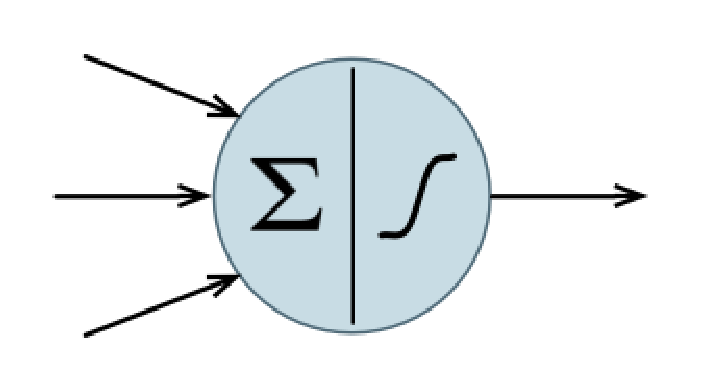
\includegraphics[height=4cm,
    angle=0]{./images/node_neuralnet.eps}}
\caption{A typical unit/node in the neural net which does weighted sum of inputs
(i.e. linear transformation) and then applied the result to a non-linear
activation function}
\label{fig:node_neuralnet}
\end{figure}


There are a whole bunch of different options available for which activation
function you use (Sect.\ref{sec:activation-function-nonlinearity}).



\begin{figure}[hbt]
  \centerline{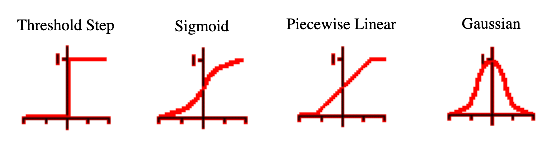
\includegraphics[height=3cm,
    angle=0]{./images/activation_functions.eps}}
\caption{Activation functions}
\label{fig:activation_functions}
\end{figure}


It used to be that you just used a sigmoid function by default, but nowadays
people use different activation functions for different purposes.
\begin{enumerate}
  \item {\bf sigmoid function}: {\bf tanh function} and {\bf logistic function}
  
  
  It models the frequency of action potentials, or firing, of biological
  neurons, i.e. it starts with small values, but can jump to a much higher value
  once it surpass a given threshold. The output is boud within a range.
  
  The first is a hyperbolic tangent that ranges from -1 to 1
 \begin{equation}
 y(u_i) = \tanh(u_i) = \frac{1}{1 + e ^{-u_i}}
 \end{equation}
 
  the other is the logistic function, which is similar in shape with tanh
  function but ranges from 0 to 1.

  \item {\bf ReLU function}
  
  The rectifier linear unit (ReLU) is more frequently used as one of the
  possible ways to overcome the numerical problems related to the sigmoids.
  
  
  \item {\bf  rectifier and softplus functions}
  
  \item {\bf radial basis functions} (more specialized activation function)
\end{enumerate}

\section{Multilayer perceptron ($\ge 1$ hidden layer)}

A multilayer perceptron (MLP) is a class of feedforward artificial neural
network (ANN).  An MLP consists of at least three layers of nodes: an input
layer, a hidden layer and an output layer.

Multilayer perceptrons are sometimes colloquially referred to as "vanilla" 
neural networks, especially when they have a single hidden layer.

Except for the input nodes, each node is a neuron that uses a nonlinear
activation function. MLP utilizes a supervised learning technique called
backpropagation for training.

\begin{figure}[hbt]
  \centerline{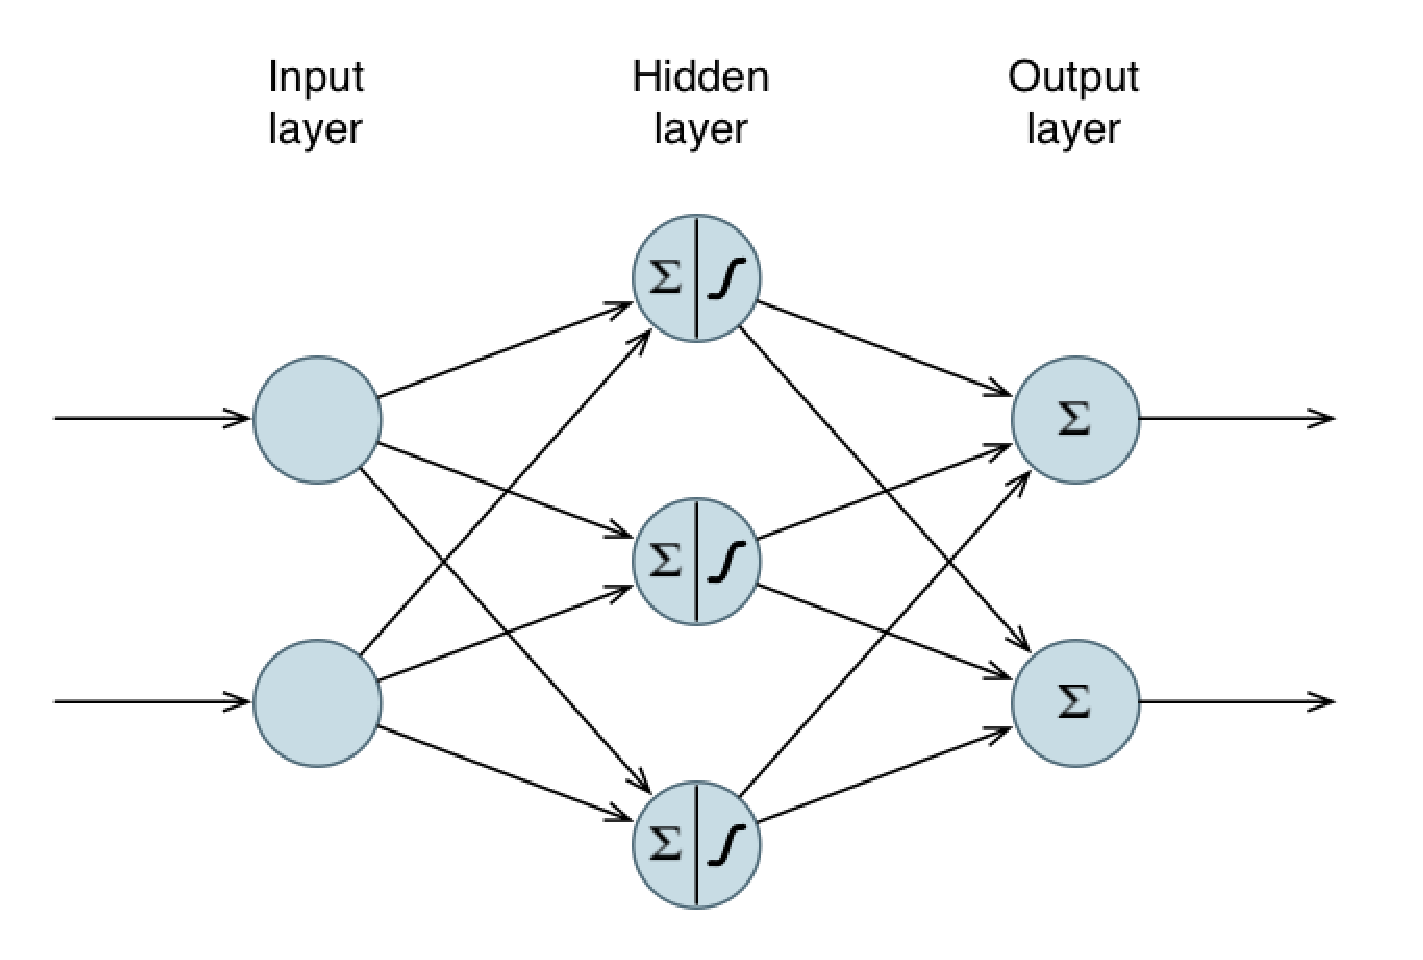
\includegraphics[height=6cm,
    angle=0]{./images/perceptron_neuralnet.eps}}
\caption{A feed-forward neural net, in that the bias is suppressed}
\label{fig:perceptron_neuralnet}
\end{figure}

\subsection{McCulloch-Pitts neuron (1943)}

 Warren McCulloch and Walter Pitts  in their 1943 paper, "A Logical Calculus of
 Ideas Immanent in Nervous Activity," contended that neurons with a binary
 threshold activation function were analogous to first order logic sentences.
 \begin{equation}
y = \phi \left( \sum_{i=1}^n w_i x_i \right)
 \end{equation}
\textcolor{red}{IMPORTANT}:  It only allowed for binary inputs and outputs, it
only used the threshold step activation function and it did not incorporate
weighting the different inputs.

\begin{mdframed}

Because of that, it has some serious limitation. In particular, there is no
threshold we can find to solve neither the “exclusive or” function (XOR), nor
the “exclusive nor” function (XNOR).

\end{mdframed}

 The McCulloch-Pitts neuron worked by inputting either a 1 or 0 for each of the
 inputs, where 1 represented true and 0 false.
 
 Thus, in order to represent the “and” function, we set the threshold at 2.0 and
 come up with the following truth table:
 \begin{verbatim}
 x1   x0     y
 0    0      0
 1    0      0
 0    1      0
 1    1      1
 \end{verbatim}

This follows also for the “or” function, if we switch the threshold value to 1.  
 \begin{verbatim}
 x1   x0     y
 0    0      0
 1    0      1
 0    1      1
 1    1      1
 \end{verbatim}

This type of artificial neuron could also be used to solve the “not” function,
which would have only one input, as well as, the NOR and NAND functions.


\subsection{Rosenblatt neuron (1950+): McCulloch-Pitts neuron + Hebbs knowledge}

In his book in 1949, The Organization of Behavior, he proposed what has come to
be known as Hebb’s rule.  He states, “When an axon of cell A is near enough to
excite a cell B and repeatedly or persistently takes part in firing it, some
growth process or metabolic change takes place in one or both cells such that
A’s efficiency, as one of the cells firing B, is increased.”
 
Hebb was proposing not only that, when two neurons fire together the connection
between the neurons is strengthened, but also that this activity is one of the
fundamental operations necessary for learning and memory.

Frank Rosenblatt, using the McCulloch-Pitts neuron and the findings of Hebb,
went on to develop the first perceptron, in that the weight between two
connected neurons can be modified. Thus, an input of 1 may be given more or less
weight, relative to the total threshold sum.

Example: A perceptron has a total of five inputs a1 through a5 with each having
a weight of w1 through w5.

The activation function used by McCulloch and Pitts was the threshold step
function.  However, other functions that can be used are the Sigmoid, Piecewise
Linear and Gaussian activation functions (Sect.\ref{sec:activation-function-nonlinearity}).


\subsection{-- Perceptron neural network as a hardware unit}

A single MLP neuron is a simple linear classifier, but complex non-linear
classifiers can be built by combining these neurons into a network.

Started in 1950s, {\bf perceptron} is a simple algorithm intended to perform
binary classification; i.e. it predicts whether input belongs to a certain
category of interest or not.
Frank Rosenblatt, godfather of the perceptron, popularized it as a device rather
than an algorithm. Rosenblatt, a psychologist who studied and later lectured at
Cornell University, received funding from the U.S. Office of Naval Research to
build a machine that could learn. His machine, the Mark I perceptron, looked
like this. 


Rosenblatt built a single-layer perceptron. It was, therefore, a shallow neural
network, which prevented his perceptron from performing non-linear
classification, such as the XOR function (an XOR operator trigger when input
exhibits either one trait or another, but not both; it stands for “exclusive
OR”), as Minsky and Papert showed in their book.

The initial hype about its performance led to a rebuttal by Minsky and Papert,
and wider spread backlash that cast a pall on neural network research for
decades.

A perceptron is a linear classifier; that is, it is an algorithm that classifies
input by separating two categories with a straight line
\begin{equation}
y = \phi \left( \sum_{i=1}^n w_i x_i + \mathbf{b} \right) = \phi\left( \mathbf{w}^T \mathbf{x} + \mathbf{b} \right)
\end{equation}
$\phi$ is the non-linear activation function.

A neural net winter that wholly thawed only with Geoff Hinton’s research in the
2000s, the results of which have since swept the machine-learning community.



\section{Radial basis network}
\label{sec:radial-basis-network}

Proposed by Broomhead and Lowe (1988) while working for  Royal Signals and Radar
Establishment, UK.

Each RBFN neuron stores a “prototype” vector which capture the 'distance' to the
input vector. Given a new input, each neuron computes the Euclidean distance
between the input and its prototype; and outputs a value between 0 and 1 which
is a measure of similarity - the output of the RBF activation function.

, and the importance of that ``prototype" is reflected via the
weight, when combining all the prototype from all hidden neurons, into making
the prediction of output label


 The shape of the RBF neuron’s response is typically a bell curve,
i.e. Gaussian function. The neuron’s response value is also called its
“activation” value.

The score is computed by taking a weighted sum of the activation values from
every RBF neuron. By weighted sum we mean that an output node associates a
weight value with each of the RBF neurons (that it receives the connection), and
multiplies the neuron’s activation by this weight before adding it to the total
response.  Every output node has its own set of weights. {\it The output node
will typically give a positive weight to the RBF neurons that belong to its
category, and a negative weight to the others.}

Roughly speaking, if the input more closely resembles the class A prototypes
than the class B prototypes, it is classified as class A.

Radial basis function (RBF) networks typically have three layers: an input
layer, a hidden layer with a non-linear RBF activation function and a linear
output layer.
\begin{itemize}
  \item input vector ($n$ units): $\mathcal{R}^n$
  
  In the basic form all inputs are connected to each hidden neuron.

  \item hidden layer: $N$ hidden neurons (known as RBF neurons)
  
  Each RBF neuron behaves like a Gaussian function, with the center represents
  the {\bf prototype} it represents. A Gaussian function has the form
  \begin{equation}
  f(x) = \frac{1}{\sigma \sqrt{2\pi}} e^{-\frac{(x-\mu)^2}{2\sigma^2}}
  \end{equation}
  
  For the activation function, $\phi$, we aren’t directly interested in the
  value of the standard deviation, $\sigma$, so we make a couple simplifying
  modifications 
  \begin{itemize}
    \item remove the coefficient: this term normally controls the height of the Gaussian

  Here, without the scaling coefficient, the function produces output in the range 0 to 1.
      
   In fact, the height is also controled with the weights applied by the output
   nodes.
   During training, the output nodes will learn the correct coefficient or
   “weight” to apply to the neuron’s response.
     
    \item replace the inner coefficient  $\frac{1}{2 * \sigma^2)}$, with a
    single parameter ‘beta’.
    
    This beta coefficient controls the width of the bell curve.
  \end{itemize}
  
  and turning that into a RBF activation function as
  \begin{equation}
  \phi(x) = e^{-\beta || x - \mu||^2}
  \end{equation}
  
  The double bar notation in the activation equation indicates that we are
  taking the Euclidean distance between x and mu, and squaring the result.
 
\begin{mdframed}

Each RBF neuron will produce its largest response when the input is equal to the prototype vector
As we move out from the prototype vector, the response falls off exponentially.

In an all-to-all connection, every RBF neuron in the network will have some
influence over the classification decision.
The exponential fall off of the activation function, however, means that the
neurons whose prototypes are far from the input vector will actually contribute
very little to the result.

\end{mdframed} 
  
  \item output: a scalar value $\mathcal{R}$
  
  
  \item the activation function for a given hidden unit $i$-th depends on the
  relative distance of that unit t with the center hidden unit
  
  The center vectors $c_i$ of the RBF functions in the hidden layer are chosen.
  This step is unsupervised, and can be performed in several ways; centers can
  be randomly sampled from some set of examples, or they can be determined using
  k-means clustering.
  
  
\end{itemize}


The training process for an RBFN consists of selecting three sets of parameters:
the prototypes (mu) and beta coefficient for each of the RBF neurons, and the
matrix of output weights between the RBF neurons and the output nodes.

\textcolor{red}{The norm is typically taken to be the Euclidean distance (although the
Mahalanobis distance appears to perform better in general)}


APPLICATION:  function approximation, time series prediction, classification, and system control. 

\url{https://mccormickml.com/2013/08/15/radial-basis-function-network-rbfn-tutorial/}

\subsection{how many RBF neurons, i.e. number of prototypes?}

An RBFN can define any arbitrarily complex decision boundary. In other words,
you can always improve its accuracy by using more RBF neurons.
Remember that each RBF neuron encodes one prototype. So the number of prototypes
equatls to the number of hidden RBF neurons.

What it really comes down to is a question of efficiency–more RBF neurons means
more compute time, so it’s ideal if we can achieve good accuracy using as few
RBF neurons as possible.


One of the approaches for making an intelligent selection of prototypes is to
perform k-Means clustering on each category samples from your training set and
to use the cluster centers as the prototypes.

How many clusters to pick per class has to be determined “heuristically”. Higher
values of k mean more prototypes, which enables a more complex decision boundary
but also means more computations to evaluate the network.

Example: I ran k-means clustering with a k of 10 twice, once for the first
class, and again for the second class, giving me a total of 20 clusters.


\subsection{ select $\beta$ (beta)}


If you use k-means clustering to select your prototypes, then one simple method
for specifying the beta coefficients is to set sigma equal to the average
distance between all points in the cluster and the cluster center.
\begin{equation}
\sigma = \frac{1}{m} \sum_{i=1}^m ||x_i - \mu||
\end{equation}
$\mu$ is the cluster centroid, m is the number of training samples belonging to this cluster

$\beta = \frac{1}{2 \sigma^2}$

\subsection{ learn output weights}


The final set of parameters to train are the output weights. These can be
trained using gradient descent (also known as least mean squares).

First, for every data point in your training set, compute the activation values
of the RBF neurons. These activation values become the training inputs to
gradient descent.

\subsection{Disadvantage of RBF network?}


The size of the RBFs network were always trained by k-means.


When your input is an image of size 128x128x3=50,000 inputs.

\url{https://www.cc.gatech.edu/~isbell/tutorials/rbf-intro.pdf}


\section{Convolutional Neural Network}
\label{sec:convolutional-neural-network}


In a nutshell, Convolutional Neural Networks (CNN's) are multi-layer neural
networks (sometimes up to 17 or more layers) that assume the input data to be
images. 

\url{http://cs231n.github.io/convolutional-networks/}


Consider you have an input, which can be 2D image or 3D images. 
\begin{verbatim}

INPUT [32x32x3] will hold the raw pixel values of the image, 
      in this case an image of width 32, height 32, 
      and with three color channels R,G,B.


\end{verbatim}

This input is
passed into the first layer, each node in the layer {\bf see} portion of the image, e.g.
\begin{itemize}
  \item one node handle 1 pixel
  
  \item one node handle 3x3 pixels 
  
  \item one node handle 5x5 pixels
\end{itemize}
Each one corresponds to a covolution operator.

\begin{verbatim}
CONV layer will compute the output of neurons that are connected to 
     local regions in the input, 
     each computing a dot product between their weights and a small region 
     they are connected to in the input volume. 
     
     This may result in volume such as [32x32x12] 
     if we decided to use 12 filters.

\end{verbatim}

NOTE: After one CONV, we can apply
\begin{verbatim}
RELU layer will apply an elementwise activation function, 
      such as the max(0,x) thresholding at zero. 
      This leaves the size of the volume unchanged ([32x32x12]).

POOL layer will perform a downsampling operation along 
     the spatial dimensions (width, height), 
     resulting in volume such as [16x16x12].

\end{verbatim}

Note that some layers contain parameters (bias, weights) and/or hyperparameters
(stride, zero padding, number of filters, etc.) and other don’t.
\begin{itemize}
  
  \item those with parameters: CONV/FC layers perform transformations that are a
  function of not only the activations in the input volume, but also of the
  parameters (the weights and biases of the neurons). The RELU/POOL layers will
  implement a fixed function.
  
 
  \item those with hyperparameters: Each Layer may or may not have additional
  hyperparameters (e.g. CONV/FC/POOL do, RELU doesn’t)
  
\end{itemize}

NOTE:
\begin{itemize}
  
  \item  There are a few distinct types of Layers (e.g. CONV/FC/RELU/POOL are by far the most popular)

  \item Each Layer accepts an input 3D volume and transforms it to an output 3D
  volume through a differentiable function.
  
\end{itemize}

\subsection{logits, i.e. the softmax argument}
\label{sec:logits}


After multiple layers, each apply one {\bf convolution filter} on one or many
elements in the incoming-input, we can convert them into a N-dimensional vector
of real-values. 
\begin{verbatim}

FC (i.e. fully-connected) layer will compute the class scores, 
        resulting in volume of size [1x1x10] 
        in the case of MNIST-image, 
        
        where each of the 10 numbers correspond to a class score, 
        such as among the 10 categories of CIFAR-10. 
        
        As with ordinary Neural Networks and as the name implies, 
        each neuron in this layer will be connected to 
        all the numbers in the previous volume.

\end{verbatim}

Typically, this is N-LABELS-dimensional vector. This is known as the {\bf
logits}. The logit at node-i, representing the node to class-i (i.e. the label $i$)
\begin{equation}
a_i = b_i + \sum_k W_{ki} h 
\end{equation}
with $b_i$ is the bias to node-i, and $W_{ki}$ is all the weights into node-i.

\begin{equation}
\mathbf{a = W^T . x} + b
\end{equation}

\begin{mdframed}

When multiple inputs is organized as a one batch, we have matrix form, the
output of one layer is written as $Z$

\begin{equation}
\mathbf{Z = X.W + b}
\end{equation}

\begin{verbatim}
X = np.array([[0.1, 0.5],
              [1.1, 2.3],
              [-1.1, -2.3],
              [-1.5, -2.5]])

W = np.array([[0.1, 0.2, 0.3],
              [0.1, 0.2, 0.3]])

bias = np.array([0.01, 0.1, 0.1])

def net_input(X, W, b):
    return (X.dot(W) + b)
    
def softmax(z):
    return (np.exp(z.T) / np.sum(np.exp(z), axis=1)).T
    
def to_classlabel(z):
    return z.argmax(axis=1)
\end{verbatim}
\end{mdframed}

In vector form, all of them form the vector of softmax argument
\begin{equation}
\mathbf{a} = (a_1, a_2, \ldots, a_N)^T
\end{equation}

\subsection{Softmax}
\label{sec:softmax}


Softmax function takes the logits vector as argument (Sect.\ref{sec:logits}),
i.e. an N-dimensional vector of real numbers, and transforms it into a vector of
real number in range (0,1) which add upto 1.

The probability for the input to be in class-i, or label $i$, i.e. as predicted by the DNN 
\begin{equation}
S_i = p_i(\mathbf{a}) = \frac{e^{a_i}}{\sum_{k=1..N}e^{a_k}}
\end{equation}

\begin{mdframed}

In practice, to make our softmax function numerically stable, i.e. avoid the
case of large $a_k$ which can make the exponent calculation unstable, we can
rescale or shift every logit to the range: negative to zero
\begin{equation}
a_j = a_j + (- \max(a_1, a_2, \ldots, a_N))
\end{equation}

NOTE: Negatives with large exponents saturate to zero rather than the infinity.


\end{mdframed}

The softmax vector, representing probabilities for all class-label, is
\begin{equation}
\mathbf{p(a)} = (p_1(\mathbf{a}), \ldots, p_N(\mathbf{a}))^T
\end{equation}

\begin{mdframed}


NOTE: softmax function is a “soft” version of max function, as instead of
selecting one maximum value, it breaks the whole (1) with maximal element
getting the largest portion of the distribution, but other smaller elements
getting some of it as well.

The softmax() part simply normalises your network predictions so that they can
be interpreted as probabilities. The softmax function outputs a categorical
distribution over outputs. By outputing a probability distribution makes softmax
suitable for probabilistic interpretation in classification tasks.

\end{mdframed}

\subsection{Loss: gradient descent via softmax}
\label{sec:loss-DNN-softmax}

Now you need to map to the concept of {\bf loss}, i.e. how well is that
prediction compared to the grouth truth, i.e. the {\bf one-hot vector} (with
only one element get value 1, and all others get value 0).

So, now you have two vectors. Suppose that you have N=6 labels
\begin{itemize}
  \item one-hot vector $y$, e.g. [0, 0, 1, 0, 0, 0]
  
   Here: the expected label value is 3 for the given input.
   
  \item softmax vector $\hat{y}=\mathbf{p(a)}$, e.g. [0.1, 0.3, 0.5, 0.01, 0.04, 0.05]
\end{itemize}

The distance between what the model believes the output distribution should be,
i.e. $\hat{y}$, and what the original distribution is, i.e. $y$, can be represented using a number of choices

\begin{enumerate}
  \item {\bf squared error}
  
  
  \item {\bf cross-entropy loss}
\end{enumerate}

\subsection{-- squared error loss}
\label{sec:loss-squared-error-softmax}
 
Squared loss
\begin{equation}
L(\mathbf{a}) = L(\mathbf{p(a), y}) = \sum_{k=1}^N \left( p_k(\mathbf{a}) - y_k \right)^2
\end{equation}

Now we need to get the derivative of the loss w.r.t. a particular softmax argument $a_i$. 
\begin{equation}
\begin{split}
\frac{\partial}{\partial a_i}L(\mathbf{a}) = \\
\frac{d}{da_i}L(\mathbf{p(a), y})  &= 
   \sum_k \frac{d}{da_i}\left( p_k(\mathbf{a}) - y_k \right)^2 \\
   &= \sum_k \frac{d}{da_i}\left( p^2_k(\mathbf{a}) - 2 \times p_k(\mathbf{a}) \times y_k + y^2_k \right) \\
   &= \sum_k \left[ 2 \times p_k(\mathbf{a}) \times \frac{\partial S_k}{\partial a_i} - 2 \times \frac{\partial S_k}{\partial a_i} \times y_k  \right] \\
   &= \sum_k 2 \times \frac{\partial S_k}{\partial a_i} \left[ p_k(\mathbf{a})  - y_k  \right] \\
   &= \sum_k 2 \times p_k(\mathbf{a}) \times (\delta_{ki} - p_i(\mathbf{a})) \left[ p_k(\mathbf{a})  - y_k  \right] 
\end{split}
\end{equation}
This is called the {\bf primary Gradients} in MGS code.

\url{https://stats.stackexchange.com/questions/153285/derivative-of-softmax-and-squared-error}


On a single training input sample $n$, the error at output nodes/units $k$-th is
\begin{equation}
\frac{\partial E}{\partial o_k^{(n)}} = o_k^{(n)} - t_k^{(n)}
\end{equation}
with $t_k$ is the element in the one-hot vector of expected output; 
$o_k$ is the value as the softmax output


\subsection{-- cross entropy loss}
\label{sec:loss-cross-entropy-softmax}

Cross entropy indicates the distance between what the model believes the output
distribution should be, and what the original distribution really is.
It is used when node activations can be understood as representing the
probability that each hypothesis might be true, i.e. when the output is a
probability distribution

When you compute the cross-entropy over two categorical distributions, this is
called the “cross-entropy loss”. Cross entropy measure is a widely used
alternative of squared error (Sect.\ref{sec:loss-squared-error-softmax}).

\begin{equation}
L(\mathbf{w}) = H(\mathbf{\hat{y}}, \mathbf{y}) = - \sum_{k=1}^N y_k \log(p_k)
\end{equation}

\begin{mdframed}
In batch training, we often see the above divided by $n$, which is batch size

\begin{equation}
L(\mathbf{w}) = \frac{1}{n} \sum_{i=1}^n H(\mathbf{\hat{y_i}}, \mathbf{y_i})
\end{equation}
or $n$ training samples.
\end{mdframed}


Now we need to get the derivative of the loss w.r.t. a particular softmax argument $a_i$. 
\begin{equation}
\begin{split}
\frac{\partial}{\partial a_i}L(\mathbf{a}) &= - \sum_{k=1}^N y_k \frac{\partial}{\partial a_i}\log(p_k) \\
   &= - \sum_{k=1}^N y_k \frac{\partial \log(p_k)}{\partial p_k} \times \frac{\partial p_k}{\partial a_i}\\
   &= - \sum_{k=1}^N y_k \frac{1}{p_k} \times \frac{\partial p_k}{\partial a_i} \\
   &= - \sum_{k=1}^N y_k \frac{1}{p_k} \times p_k \times (\delta_{ki} - p_i) \\
   &= - \sum_{k=1}^N y_k \times (\delta_{ki} - p_i) \\
   &= - y_i (1 - p_i) + \sum_{k \ne i} y_k \times p_i \\
   &= p_i \times (y_i + \sum_{k \ne i} y_k) - y_i \\
   &= p_i - y_i
\end{split}
\end{equation}
which is a very simple and elegant expression. This is called the {\bf primary Gradients} in MGS code.

NOTE: $\delta_{ki} = 1$ if $k==i$, and 0 otherwise. 
\url{https://deepnotes.io/softmax-crossentropy}.

% Once your network is predicting a probability distribution over labels for each
% input, the log loss is equivalent to the cross entropy between the true label
% distribution and the network predictions.
%  
% 
% N-dimensional softmax is often used as the final layer in neural networks.
% The gradient of softmax with respect to its inputs is really the partial of each
% output with respect to each input
% 
% 
% For this we need to calculate the derivative or gradient and pass it back to the
% previous layer during backpropagation.

REMEMBER:
\begin{itemize}
  \item softmax $p_i$ is calcualted at the output layer
  
  \item logits $a_i$ is calculated at the outter most hidden layer
\end{itemize}

REMEMBER:
\begin{equation}
a_i = \sum_{j=1}^M h_j w_{ji}
\end{equation}
with $h_j$ is the result of the transfer function from the node $j$-th in the previous layer.

Given weight $w_{ji}$ connecting the current hidden node $i$-th to the output softmax node $j$-th.
The derivative of the error with respect to each weight connecting the hidden units
to the output units using the chain rule
\begin{equation}
\begin{split}
\frac{\partial L}{\partial w_{ji}} &= \frac{\partial L}{\partial p_i} \frac{\partial p_i}{\partial a_i} \frac{\partial a_i}{\partial w_{ji}} \\
 &= (p_i - y_i) \times h_j
\end{split}
\end{equation}
with $h_j$ is the activation function's value at hidden unit $j$-th, e.g. tanh function. 

So, the weight is updated using the rule
\begin{equation}
w_j := w_j + \eta \times \frac{\partial L}{\partial w_{ji}}
\end{equation}

The bias is also updated
\begin{equation}
b_j := b_j + ()
\end{equation}
\url{http://rasbt.github.io/mlxtend/user_guide/classifier/SoftmaxRegression/}

\subsection{Derivative of a softmax}

The information below is used to help calculating the loss (Sect.\ref{sec:loss-DNN-softmax}).

For the j-th element of softmax, its derivative w.r.t the i-th element of input is
\begin{equation}
\frac{\partial S_j}{\partial a_i} = \frac{\partial p_j}{\partial a_i} = \frac{g/h}{\partial a_i}
\end{equation}
with $g = e^{a_j}$ and $h = \sum_{k=1..N}(e^{a_k})$.

NOTE:
\begin{equation}
S_j = p_j(\mathbf{a}) = \frac{e^{a_j}}{\sum_{k=1..N}e^{a_k}}
\end{equation}


NOTE: From quotient rule: given f(x) = g(x)/h(x), then
\begin{equation}
f'(x) = \frac{ g'.h - g.h'}{h(x)^2}
\end{equation}

\begin{itemize}
  
  \item In h(.): then $\frac{\partial h}{\partial a_i} = e^{a_i}$
  
  \item In g(.)): then $\frac{\partial g}{\partial a_i} = e^{a_i} (\delta_{ji})$
  
  and  Kronecker delta $\delta_{ji} = 1$ if j=i, and is equal to 0 elsewhere.
\end{itemize}

Finally, the result is
\begin{equation}
\frac{\partial S_j}{\partial a_i} = p_j \times (\delta_{ji} - p_i)
\end{equation}
and $\delta_{ji} = 1$ if j=i, and is equal to 0 elsewhere.

% So, the total-gradient that the input $j-$th receives is the sum of partial
% derivative w.r.t that input element.
% 
% 
% In summary:
% \begin{itemize}
%   \item f()
% \end{itemize}

\subsection{Loss: gradient descent via sigmoid}
\label{sec:loss-DNN-sigmoid}


For the input value $a_i$, the sigmoid output 
\begin{equation}
h_{\theta} (a_i) =  \frac{\mathrm{1} }{\mathrm{1} + e^{-\theta^Ta_i} } 
\end{equation}

In this architecture, the outputs are computed by applying the logistic function
to the weighted sums of the hidden layer activations,
\begin{equation}
a_i = \sum_{j} h_j \times w_{ji}
\end{equation}
with $h_j$ is the values in nodes of the hidden layer right before the output layer.


The loss for a given node-i has no dependence on other nodes $j$.
\begin{enumerate}
  \item squared error loss
\end{enumerate}

\subsection{-- squared error loss}


If sigmoid is being used to derive proprability for label-i to be predicted, the squared error loss is

\begin{equation}
\frac{d}{da_i}L(\mathbf{p(a), y})  &= 2 \times (\mathbf{p}(\mathbf{a}) - \mathbf{y} ) \odot \mathbf{p} \odot (1 - \mathbf{p})
\end{equation}

\subsection{-- cross entropy loss}

Similar to that in softmax, the gradient is computed and gives the same formula
\begin{equation}
\frac{\partial L}{\partial w_{ji}} = p_i - y_i
\end{equation}

Note that this is the same formula as in the case with the logistic output units! The values themselves
will be different, because the predictions $p_i$ will take on different values depending on whether the
output is logistic or softmax, but this is an elegant simplification.
 

On a single training input sample $n$, the error at output nodes/units $k$-th is
\begin{equation}
\frac{\partial E}{\partial o_k^{(n)}} = o_k^{(n)} - t_k^{(n)}
\end{equation}
with $t_k$ is the element in the one-hot vector of expected output; 
$o_k$ is the value as the logistic activation function's output

\begin{equation}
o_k^{(n)} = g(z_k^{(n)}) = \frac{1}{1 + \exp(z_k^{(n)})}
\end{equation}

So,
\begin{equation}
\frac{\partial o_k^{(n)}}{\partial z_k^{(n)}} = o_k^{(n)} \left( 1 - o_k^{(n)} \right)
\end{equation}

$w_{ki}$ is the weight connecting from node $i$ to node $k$. Then, the error gradient is
\begin{equation}
\frac{\partial E}{\partial w_{ki}} = \frac{\partial E}{\partial o_{k}} \times \frac{\partial o_k}{\partial z_{k}} \times \frac{\partial z_k}{\partial w_{ki}}
\end{equation}
\url{https://www.cs.toronto.edu/~urtasun/courses/CSC411/10_nn1.pdf} (Slide 15)

NOTE:
\begin{enumerate}
  \item the error between the expected output and predicted
  
\begin{equation}
\frac{\partial E}{\partial o_{k}} = o_k^{(n)} - t_k^{(n)}
\end{equation}
with $o_k^{(n)}$ is the output of the last activation function, e.g. softmax or logistic function, based on the input sample at index (n)
of the training batch.

  \item 
\end{enumerate}



\section{GAN (Generative Adversial Network)}
\label{sec:GAN}

GANs are an interesting idea that were first introduced in 2014 by a group of
researchers at the University of Montreal lead by Ian Goodfellow (now at OpenAI).

GAN (Generative Adversial Network) uses 2 networks.
One neural network, called the \verb!generator!, generates new data instances,
while the other, the \verb!discriminator!, evaluates them for authenticity; i.e.
the discriminator decides whether each instance of data it reviews belongs to the
actual training dataset or not.


Example: consider MNIST dataset (of handwriting digits).
The goal of the discriminator, when shown an instance from the true MNIST
dataset, is to recognize them as authentic.

The generator will try its best in creating new images that it passes to the
discriminator. It does so in the hopes that they, too, will be deemed authentic,
even though they are fake.

You need to train both networks.
However, when you train the discriminator, hold the generator values constant;
and when you train the generator, hold the discriminator constant.
Pretraining the discriminator against MNIST before you start training the
generator will establish a clearer gradient.


GANs take a long time to train. On a single GPU a GAN might take hours, and on a
single CPU more than a day.






\section{Autoencoder-like network}
\label{sec:autoencoder}


An autoencoder neural network is an unsupervised learning algorithm that
applies backpropagation, setting the target values to be equal to the inputs,
with a reconstruction objective.

i.e. a set of unlabeled training data samples
\begin{equation}
{ x^{(1)}, x^{(2)}, \ldots}, \qquad \text{ where} x^{(i)} \in R^n
\end{equation}

\section{Paired feedforward networks}

Paired feedforward networks with a correlation-based objective.


\section{Recurrent neural network}
\label{sec:recurrent-neural-network}


\section{Discrimitive algorithms vs. Generative algorithms}

\subsection{discrimitive algorithm: p(y|x)}
\label{sec:discrimitive-algorithm}

Discriminative algorithms map features to labels. Any discrimitive algorithm can
be represented in the form of \verb!p(y | x)!, i.e. what is the probability for
predicting the label 'y' given the feature data 'x'.

For example, given all the words in an email, a discriminative algorithm could
predict whether the message is \verb!spam! or \verb!not_spam!. \verb!spam! is
one of the labels, and the bag of words gathered from the email are the features
that constitute the input data

The formulation p(y|x) is used to mean "the probability of y given x", which in
this case would translate to "the probability that an email is spam given the
words it contains."

\subsection{Generative algorithm}
\label{sec:generative-algorithm}
One way to think about generative algorithms is that they do the opposite.
Instead of predicting a label given certain features, they attempt to predict
features given a certain label.

Mathematically, they allow you to capture \verb!p(x|y)!, the probability of x
given y, or the probability of features given a class. 
Generative models care about "how you get x."

\begin{mdframed}
That said, generative algorithms can also be used as classifiers. It just so
happens that they can do more than categorize input data.
\end{mdframed}

\section{Reinforcement learning}

\section{Deep neural network}
\label{sec:deep-neural-network}


Deep neural networks are the new default machine learning approach in many
domains, such as computer vision, speech processing, and natural language
processing.

Given sufficient data for a target task, end-to-end models can be learned with
fairly simple, almost universal algorithms. Such models learn their own internal
representations, which in many cases appear to be similar to human-engineered
ones.

Karen Lievescu asked the question whether domain-knowledge is still needed?
\url{https://www.eecs.umich.edu/eecs/etc/events/showevent.cgi?4557}


\section{Loss function}

\subsection{Connectionist Temporal Classification (CTC)
loss function}
\label{sec:CTC-loss-function}

Neural networks trained with the Connectionist Temporal Classification (CTC)
loss function [22] to predict speech transcriptions from audio - Sect.\ref{sec:DS2-Baidu}


\chapter{Datasets: Deep Learning}


Top 50 datasets:
\url{https://bytescout.com/blog/datasets-machine-learning.html}

\section{MNIST}
\label{sec:dataset-digits-MNIST}

MNIST (LeCun.Bottou.Bengio.ea.1998) contains 60,000 images for training and
10,000 images for validation.

Each image contains a handwritten digit from 0 to 9. The task is classifying
each image into the corresponding digit.
Each image is a grayscale image with both width and height of $28$ with shape ($28$,$28$,$1$).
In addition, the dataset represents each pixel by a unsigned $8$-bit integer.

Provided by libraries:

\begin{itemize}
  \item  Gluon provides a MNIST class in the data.vision module to automatically retrieve the dataset from the internet. 

Subsequently, Gluon will use the already-downloaded local copy. 

We specify whether we are requesting the training set or the test set by setting
the value of the parameter train to True or False, respectively.

We use a customized transformation to remove the last channel dimension; and
quantize them into binary features (in range [0, 1]) to simplify the problem.
 
\begin{lstlisting}
def transform(data, label):
    return np.floor(data.astype('float32') / 128).squeeze(axis=-1), label

mnist_train = gluon.data.vision.MNIST(train=True, transform=transform)
mnist_test = gluon.data.vision.MNIST(train=False, transform=transform)

image, label = mnist_train[2]
image.shape, label


image.shape, image.dtype

label, type(label), label.dtype


images, labels = mnist_train[10:38]
images.shape, labels.shape

d2l.show_images(images, 2, 9);
\end{lstlisting}



  \item 
\end{itemize}


\section{openFDA: }

\url{https://www.ibmbigdatahub.com/blog/exploring-public-open-data-project-part-1}

provides public access to FDA data, including reports on adverse drug events


\chapter{Applications of Machine Learning}
\label{sec:application-machine-learning}

\section{Seconds}

\subsection{Spam detection}

\subsection{Price optimization}

\subsection{Cross selling}


\subsection{Fraud detection}

\subsection{Search result/product recommendation}


\subsection{Picture detection}

\section{Minutes}


\subsection{Transportation rerouting}


\subsection{Customer services}


\section{Hours}




\subsection{Predictive management}

\subsection{Inventory management}

 

\chapter{Automatic speech recognition (ASR)}

Decades worth of hand-engineered domain knowledge has gone into current state-of-the-art ASR pipelines.

One of the challenges of speech recognition is the wide range of variability in
speech and acoustics.
As a result, modern ASR pipelines are made up of numerous components including
complex feature extraction, acoustic models, language and pronunciation models,
speaker adaptation, etc. Building and tuning these individual components makes
developing a new speech recognizer very hard, especially for a new language.
Indeed, many parts do not generalize well across environments or languages.


Using deep learning, recent efforts to deploy ASR models end-to-end, it is
expected to replace most modules with a single model.

\section{ Deep Speech 2 ASR pipeline (Baidu)}
\label{sec:DS2-Baidu}

Deep Speech 2 (DS2) is an end-to-end deep learning system, with 3 main
components:
the model architecture, large labeled training datasets, and computational
scale.

Deep Speech 2 ASR pipeline approaches or exceeds the accuracy of Amazon
Mechanical Turk human workers on several benchmarks, works in multiple languages
with little modification, and is deployable in a production setting.

\url{https://arxiv.org/pdf/1512.02595v1.pdf}

They searched a proper deep network architecture by testing with
\begin{enumerate}
  \item  Neural networks trained with the Connectionist Temporal Classification (CTC)
loss function [22] to predict speech transcriptions from audio

  \item networks composed of many layers of recurrent connections, convolutional filters, and nonlinearities

  \item the impact of a specific instance of Batch Normalization [63] (BatchNorm) applied to RNNs

\end{enumerate}

The authors found networks that produce much better predictions than those in previous
work [26], but also find instances of recurrent models that can be deployed in a
production setting with no significant loss in accuracy.

\begin{mdframed}

Our English speech system
is trained on 11,940 hours of speech, while the Mandarin system is trained on 9,400 hours. We use
data synthesis to further augment the data during training

Models are larger, i.e. many more parameters than those used in our previous
system. Training a single model at these scales requires tens of exaFLOPs1 that
would require 3-6 weeks to execute on a single GPU.

This makes model exploration a very time consuming exercise, so we have built a
highly optimized training system that uses 8 or 16 GPUs to train one model. 
This scalability and efficiency cuts training times down to 3 to 5 days,
allowing us to iterate more quickly on our models and datasets

TRICKS:
\begin{enumerate}

  \item  In contrast to previous large-scale training
approaches that use parameter servers and asynchronous updates [18, 10], we use
synchronous SGD, which is easier to debug while testing new ideas, and also
converges faster for the same degree of data parallelism
  
  \item optimizations for a single GPU
as well as improvements to scalability for multiple GPUs

  \item e optimizations include a fast implementation of the CTC loss function
  on the GPU, and a custom memory allocator

  \item carefully integrated compute nodes and a custom implementation of all-reduce to accelerate
inter-GPU communication.

\end{enumerate}
Overall the system sustains approximately 50 teraFLOP/second when
training on 16 GPUs. This amounts to 3 teraFLOP/second per GPU which is about 50\% of peak
theoretical performance

\end{mdframed}


\section{Amazon Mechanical Turk}

\chapter{Install DeepLearning}


CUDA driver direct download link:
\url{https://developer.nvidia.com/cuda-downloads?target_os=Linux&target_arch=ppc64le&target_distro=Ubuntu&target_version=1804&target_type=runfilelocal}
\begin{verbatim}

wget http://developer.download.nvidia.com/compute/cuda/10.2/Prod/local_installers/cuda_10.2.89_440.33.01_linux_ppc64le.run
sudo sh cuda_10.2.89_440.33.01_linux_ppc64le.run

\end{verbatim}

\chapter{PyTorch}

c10/cuda is a core library with CUDA functionality. It is distinguished from c10
in that it links against the CUDA library.
\url{https://github.com/pytorch/pytorch/tree/master/c10/cuda}

Like c10 it doesn't contain any kernels, and consists solely of core
functionality that is generally useful when writing CUDA code; for example, C++
wrappers for the CUDA C API.

The code in this folder is very special, because on our AMD GPU build, we
transpile it into c10/hip to provide a ROCm environment.

Example: user code
\begin{lstlisting}
// c10/cuda/CUDAFoo.h
namespace c10 { namespace cuda {

void my_func();

}}
\end{lstlisting}
is transpiled into
\begin{lstlisting}
// c10/hip/HIPFoo.h
namespace c10 { namespace hip {

void my_func();

}}
\end{lstlisting}



\chapter{Caffe}

\section{matcaffe}
\label{sec:matcaffe}

matlab wrapper of caffe aka matcaffe 
\begin{verbatim}
export LD_PRELOAD=/usr/lib/x86_64-linux-gnu/libstdc++.so.6

export
LD_PRELOAD=$LD_PRELOAD:/usr/lib/x86_64-linux-gnu/libstdc++.so.6:/usr/lib/x86_64-linux-gnu/libprotobuf.so.9
\end{verbatim}

Note: matcaffe supports Opencv 2.4.9 , so better use it as well.

\chapter{TensorFlow (C++, Python)}
\label{sec:TensorFlow}

Google built the underlying TensorFlow software with the C++ programming
language. But in developing applications for this AI engine, coders can use
either C++ or Python.

Google is not yet open sourcing a version of TensorFlow that lets you train
models across a vast array of machines. The initial open source version only
runs on a single computer. This computer can include many GPUs, but it's a
single computer nonetheless.


TensorFlow is well suited not only to deep learning, but to other forms of AI,
including reinforcement learning (Sect.\ref{sec:reinforcement-learning}) and
logistic regression (Sect.\ref{sec:logistic-regression}).

Typically, Google trains these neural nets using a vast array of machines
equipped with GPU chips. GPUs are good at processing lots of little bits of data
in parallel, and that's what deep learning requires. After they've been
trained - when it's time to put them into action - these neural nets run in
different ways. They often run on traditional computer processors inside the
data center, and in some cases, they can run on mobile phones. 

TensorFlow has better computational graph visualizations as they provide this
natively while the equivalent in Torch/Theano isn't nearly as fun to look at.
But as for visualizing convolutional filters, images, and graphs, Theano is just
as good.


\section{Install}

\subsection{IBM Power8 (little Endian)}
\label{sec:Power8-IBM}

Anaconda on Power 8: \url{https://docs.anaconda.com/anaconda/install/}
\begin{itemize}
  \item package lists \url{https://docs.anaconda.com/anaconda/packages/pkg-docs}
  
  \item R language:
  \url{https://docs.anaconda.com/anaconda/packages/r-language-pkg-docs}
  
\end{itemize}


Tensorflow on Power 8:
\url{https://www.ibm.com/developerworks/community/blogs/fe313521-2e95-46f2-817d-44a4f27eba32/entry/Building_TensorFlow_on_OpenPOWER_Linux_Systems?lang=en}

\subsection{IBM Power9}
\label{sec:Power9-IBM}

Power9 and the E900 family of servers.

IBM rolled out various 900-class servers using the latest Power9 processor for
applications ranging from traditional cloud-based applications, typically
deployed in the scale-out model, to specialized big data and AI workloads.
Now, IBM is completing the family with the E900 servers designed to handle the
most compute and memory intensive workloads in the enterprise or the cloud.

The Power9 competes directly with Intel’s highest performance Xeon Scalable
Processors (SP) but offers up to twice the performance per core and just shy of
twice the memory bandwidth performance, making it the perfect choice for
performance-hungry, scale-up applications.



\subsection{-- (little-Endian) OpenPower Linux platform}

\url{https://openpowerfoundation.org/blogs/introducing-the-little-endian-openpower-software-development-environment-and-its-application-programming-interfaces/}


One particularly pervasive dependence is  byte ordering of data.  Byte ordering
affects both the layout of data in memory, and of disk-based data repositories.

While Power had supported both big-endian (most significant byte first) and
little-endian (least significant byte first) data orderings, common Power
environments have always used big-endian ordering, i.e. many compiled apps are
designed to run on big-endian ordering.
 
\begin{verbatim}
Imagine the number one hundred twenty three.  When representing this number with
numerals, we typically write it with the most significant digit first and the
least significant digit last: 123.  This is big endian.  Mainframes and RISC
architectures like POWER default to big endian when manipulating data.


// Intel x86
The least significant digit first and the most significant digit last: 321. 
This is little endian.  x86 architectures use little endian when storing data.
\end{verbatim}

To address endian-ness, Power8 was defined to offer the same high performance
for big- and little-endian applications. The POWER8 processor is the first
processor to support little endian and big endian modes equivalently. Although
previous generations of the POWER processors had basic little endian
functionality, they did not fully implement the necessary instructions in such a
way to enable enterprise operating system offerings.   


However, the previous Linux distributions and supporting applications, for Power
CPUs, run in big endian mode.
\begin{itemize}
  \item   Red Hat and SUSE will continue to support their existing big endian
  releases on Power for their full product lifecycles.
\end{itemize}
\url{https://www.ibm.com/developerworks/community/blogs/fe313521-2e95-46f2-817d-44a4f27eba32/entry/just_the_faqs_about_little_endian?lang=en}


As the Linux application ecosystem for x86 platforms is much larger and Linux
on x86 uses little endian mode. IBM has shifted to develop  little-endian Linux
distro on Power CPUs. 
\begin{itemize}
  \item   Canonical's Ubuntu Server 14.04 distribution supports little endian on
  Power CPUs.
  
  \item Future: add Debian and openSUSE 
  
  \item Red Hat has not yet publicly disclosed their plans around a little
  endian operating systems  
\end{itemize}

CURRENTLY:  Big endian (BE) operating systems support 32-bit and 64-bit
applications. Little endian (LE) operating systems exclusively support 64-bit
applications.
\url{https://www.ibm.com/support/knowledgecenter/en/linuxonibm/liaam/liaamdistros.htm}

To test if your current Linux distro is little endian?
\begin{verbatim}
echo -n I | od -to2 | head -n1 | cut -f2 -d" " | cut -c6 
\end{verbatim}
\url{https://serverfault.com/questions/163487/how-to-tell-if-a-linux-system-is-big-endian-or-little-endian}


Existing PowerLinux application portfolio supports only big endian modes today.
Existing third party and IBM applications will likely migrate more slowly and
deliberately.  As such, Power hardware will support both endian modes for the
foreseeable future so that existing Linux applications optimized for a big
endian platform will continue to run (of course on big-endian Linux distro)
unchanged while new applications optimized to little endian mode are added (and
of course must run on little-endian Linux distro).

Open source applications have begun extending their support to little endian
mode on Power Systems. 


\subsection{-- build TensorFlow from source}


\url{https://www.ibm.com/developerworks/community/blogs/fe313521-2e95-46f2-817d-44a4f27eba32/entry/Building_TensorFlow_on_OpenPOWER_Linux_Systems?lang=en}


To build TensorFlow, we start by building Bazel, the build tool used to build
TensorFlow binaries.

\url{https://www.tensorflow.org/install/install_sources}
\begin{verbatim}
//bazel first
// Bazel is an open-source build and test tool similar to Make, Maven, and Gradle.
echo "deb [arch=amd64] http://storage.googleapis.com/bazel-apt stable jdk1.8" | sudo tee /etc/apt/sources.list.d/bazel.list
curl https://bazel.build/bazel-release.pub.gpg | sudo apt-key add -
sudo apt-get update && sudo apt-get install bazel




git clone https://github.com/tensorflow/tensorflow 

// check the branch you want to build
// e.g. r1.0 release 
// git checkout r1.0

\end{verbatim}

\subsection{CPU only}

\url{https://www.tensorflow.org/install/install_linux}
\begin{verbatim}
conda create -n tensorflow pip python=3.3

source activate tensorflow

pip install --ignore-installed --upgrade \
 https://storage.googleapis.com/tensorflow/linux/cpu/tensorflow-1.5.0-cp34-cp34m-linux_x86_64.whl
\end{verbatim}

\subsection{CPU + GPU}

To use TensorFlow, it requires more coding (than using higher-level framework
like Keras - Sect.\ref{sec:Keras}), and for most standard designs, you will end
up writing your own layer builder and NN training routines that are not required
(to write) in Keras.

With TensorFlow knowledge, and design of NNs at the level it implements is a
nice marketable skill. It also allows you to tackle architectures and designs
outside of Keras' API, such as RBMs (assuming Keras still doesn't implement
them).


\subsection{Intel  Xeon Scalable
Processors (SP) }
\label{sec:Intel-Xeon-Scalable-Processor}

Intel  Xeon Scalable
Processors (SP) 

\chapter{Theano (Python)}
\label{sec:Theano}

Theano is a Python library that allows you to define, optimize, and evaluate
mathematical expressions involving multi-dimensional arrays efficiently. 


\chapter{Keras [:TensorFlow, Theano]}
\label{sec:Keras}

Keras is a deep-learning library that sits atop TensorFlow
(Sect.\ref{sec:TensorFlow}) and Theano (Sect.\ref{sec:Theano}), providing an
intuitive API inspired by Torch (Sect.\ref{sec:Torch}).

Keras is a deep-learning library (Sect.\ref{chap:deep-learning}) that sits atop
Theano and TensorFlow, providing an intuitive API inspired by Torch.

Keras has a simpler, almost declarative, design of the API to build an NN model.
If you want to build any standard NN architecture, either deep feed-forward, CNN
or RNN, and are focused on simply training and testing the result, then Keras is
good choice because you can probably save a few minutes writing the code. 

\chapter{Deeplearning4j [:Keras]}
\label{sec:Deeplearning4j}
%\section{Deeplearning4j: Keras}

Deeplearning4j relies on Keras as its Python API and imports models from Keras
and through Keras from Theano and TensorFlow. It was created by Francois
Chollet, a software engineer at Google. 



\section{Eclipse DL4j}
\label{sec:EclipseDL4j}

Eclipse Deeplearning4j targets enterprises looking to implement deep learning
technologies. 

Eclipse DL4J is a JVM-based, industry-focused, commercially supported,
distributed deep-learning framework that solves problems involving massive amounts of data
in a reasonable amount of time.

\url{https://projects.eclipse.org/proposals/eclipse-deeplearning4j}

\begin{verbatim}

Deeplearning4j: Neural network DSL (facilitates building neural networks
integrated with data pipelines and Spark)

ND4J: N-dimensional arrays for Java, a tensor library: "Eclipse January with C
code and wider scope". The goal is to provide tensor operations and optimized
support for various hardware platforms

DataVec: An ETL library that vectorizes and "tensorizes" data. Extract transform
load with support for connecting to various data sources and outputting
n-dimensional arrays via a series of data transformations

libnd4j: Pure C++ library for tensor operations, which works closely with the
open-source library JavaCPP (JavaCPP was created and is maintained by a Skymind
engineer, but it is not part of this project).

RL4J: Reinforcement learning on the JVM, integrated with Deeplearning4j.
Includes Deep-Q learning used in AlphaGo and A3C.

Jumpy: A Python interface to the ND4J library integrating with Numpy

Arbiter: Automatic tuning of neural networks via hyperparameter search.
Hyperparameter optimization using grid search, random search and Bayesian
methods.
\end{verbatim}


\chapter{Apache Kafka + Confluent}
\label{sec:Confluent}
\label{sec:Apache-Kafka}



\section{}

\chapter{Platforms}

\section{Skymind}

Skymind Intelligence Layer (SKIL)  gives developers an easy way to train and
deploy powerful deep learning models to production quickly and easily.
\url{https://docs.skymind.ai/docs/docker-image}

SKIL offers ETL, training and one-click deployment on a managed GPU cluster.
SKIL Community Edition is free. SKIL includes many frameworks, i.e. 13.3 GB for
Docker image.
\begin{enumerate}
  \item Deeplearning4j - Sect.\ref{sec:Deeplearning4j}
  
  \item Tensorflow - Sect.\ref{sec:Tensorflow}
  
  \item Keras - Sect.\ref{sec:Keras}
  
  \item 
\end{enumerate}


\begin{verbatim}
docker pull skymindops/skil-ce:1.0.2-2
\end{verbatim}

Example: to run
\begin{verbatim}
docker run --rm -it -p 9008:9008 -p 8080:8080 skymindops/skil-ce:1.0.2-2 bash /start-skil.sh
\end{verbatim}
a temporary container with embedded data stores, all data like notebooks will
get erased when you stop the container.

Example: to run with persistent notebooks, use Docker's volumes
\url{https://docs.docker.com/storage/volumes/}
\begin{verbatim}
// do only once

docker volume create --name zk-data
docker volume create --name zk-datalog
docker volume create --name skil-data
docker pull zookeeper
docker run --name zookeeper -v zk-data:/data -v zk-datalog:/datalog -d zookeeper
docker run --rm -it --name skil -v skil-data:/var/skil --env SKIL_EMBEDDED_DB_PATH=/var/skil/skildb --env ZOOKEEPER_EMBEDDED=false --env ZOOKEEPER_HOST=zookeeper --env ZOOKEEPER_PORT=2181 --link zookeeper:zookeeper -p 9008:9008 -p 8080:8080 skymindops/skil-ce bash /start-skil.sh

// 
docker stop skil
docker stop zookeeper


docker start zookeeper
docker run --rm -it --name skil -v skil-data:/var/skil --env SKIL_EMBEDDED_DB_PATH=/var/skil/skildb --env ZOOKEEPER_EMBEDDED=false --env ZOOKEEPER_HOST=zookeeper --env ZOOKEEPER_PORT=2181 --link zookeeper:zookeeper -p 9008:9008 -p 8080:8080 skymindops/skil-ce bash /start-skil.sh
\end{verbatim}
SKIL uses both the filesystem and zookeeper for state so the simplest way to
persist your notebooks and model server configurations is to use a separate
zookeeper container and use persistent data volumes for zookeeper and SKIL.  


and via web browser
\begin{verbatim}
 http://localhost:9008
 
 // or use the Docker's IP
 http://<IP>:9008
  
 docker ps  //to get <container ID>
 docker inspect <container ID>
\end{verbatim}
\url{https://stackoverflow.com/questions/17157721/how-to-get-a-docker-containers-ip-address-from-the-host}


\section{H2O.ai}
\label{sec:H2O.ai}

H2O.ai makes machine learning accessible and allows business users to extract
insights from data, without needing expertise in deploying or tuning machine
learning models.

H2O allows users to fit thousands of potential models as part of discovering
patterns in data; with data stored on cloud or in Apache HDFS, as well as in the
conventional operating-system Linux, Mac O/S, Windows.

The founder, Ambati was frustrated with the performance of the R programming
language on large data-sets and started the development of H2O software .

The H2O software is written in Java, Python, and R. The H2O software runs can be
called from the statistical package R, Python, and other environments, e.g. 
Apache Spark (Sect.\ref{sec:apache_spark})

\url{https://en.wikipedia.org/wiki/H2O_(software)}





\section{RapidMiner}
\label{sec:RapidMiner}


 

\chapter{Machine learning}
\label{sec:machine-learning}

Machine learning allows {\it a machine to find hidden insights without being
explicitly programmed where to look for}. See applications
(Sect.\ref{sec:application-machine-learning}).

In a traditional way, there are several applications for Machine Learning
(ML), 
\begin{enumerate}
  \item  data mining
   
  \item classification
\end{enumerate}

The classification is a fundamental problem in that machine learning techniques
have been widely used to solve;  e.g. neural networks. 


\section{Abstract a problem in mathematical language}

The most common mathematical framework for learning.
\begin{enumerate}
  \item training samples

$D$ contains a set of data item
\begin{equation}
D = {z_1, z_2, \ldots, z_n}
\end{equation}
with $z_i$ represent a completed data item and is sampled from an {\bf
unknown} process $P(Z)$. \textcolor{red}{REMEMBER that the goal is to build a
system $f$ that is (trained to behave/producing output/making decision) as
closed to (as good as) this unknown process as possible}.
  
  \item A loss functional $L$: 

\begin{equation}
L(f, z_i) = \text{real-valued scalar}
\end{equation}  

The different real-valued scalar represent the error, which we aim to minimize
by adjusting the parameters/weights of some decision function $f$.
At the end of the training, $f$ is supposed to behave like the unknown process $P$.

%There are common strategies to choose this loss function.

   \item The question is how to adjust the parameters/weights that represent the
   state function of $f$? 
   
   There are two approaches
   \begin{enumerate}
     \item super-vised learning - Sect.\ref{sec:supervised-learning}
     \item unsupervised learning - Sect.\ref{sec:unsupervised-learning}
   \end{enumerate} 
\end{enumerate}

\subsection{supervised learning}
\label{sec:supervised-learning}

Given the training samples, we always know the expected outcome, i.e. 
training samples always come in pair, $z_i=(x,y)$ with x=input,
y=target-output/decision.  NOTE: For multiple data samples, we use upper-case
symbol, i.e. $Z=(X,Y)$ - a vector/matrix.

QUESTION: minimize the difference $f(x)-y$, which is typically represented as,
depending on the type of values of $Y$.
\begin{enumerate}
  \item {\bf regression} form: if $Y$ is a real-value scalar, or vector.
  
  \begin{equation}
L(f,(X,Y)) = ||f(X)-Y||^2
\end{equation}
  
  
  \item {\bf classification} form: if $Y$ is an integer-value scalar, or a
  symbol) corresponding to a class index, i.e. category index.
  
 $f(X)$ represents a probability function, with $f_i(X)$ returns the probability
 that X falls into category $i$-th. So, the contraints are
 \begin{equation}
 \begin{split}
 \sum_i f_i(X) = 1 \\
 f_i(Y) \ge 0
 \end{split}
 \end{equation}
  
 This maps to the Bayesian decision rule: $P(Y=i | X)$. When the system
 'predict'/estimate the right category, it means that the probability for that
 should be high (as close to 1 as possible). This maps to the loss function by
 converting into the \verb!-log()! function
 \begin{equation}
 L(f, (X,Y)) = -log f_Y(X)
 \end{equation}
  
  
\end{enumerate}




\subsection{unsupervised learning}
\label{sec:unsupervised-learning}

As we don't know the target of individual data item/point, one way to find out
which data points belong to the same 'unknown' target is by 'visualizing' them
in the space, and find the clustering, i.e. those clustered together are
supposed to be of the same 'unknown' target.

This is known as {\bf density estimation}, i.e. discovering the hidden
properties inside the data. So, if we can estimate its density function
(Sect.\ref{sec:density-estimation}), i.e. we can have a good chance of
predicting the 'target' of a new data. Density estimation walks the line between
unsupervised learning, feature engineering, and data modeling.

% Consider the {\bf unknown} process $P$ whose outcome/output as a random
% variable, i.e. we don't know it's next value, but we may know its probbility
% density function, if the output is known to be clustered following certain
% distribution pattern.

 
\section{Density estimation}
\label{sec:density-estimation}

Density estimation is a very simple concept being used in unsupervised learing
(Sect.\ref{sec:density-estimation}), and most people are already familiar with
one common density estimation technique: the histogram
(Sect.\ref{sec:histogram}).


\section{Classification}
\label{sec:classification}

Classification systems play an important role in a wide variety of fields by
classifying the available information based on some criteria.
Many decision-making tasks are instances of classification problem or can be
easily formulated into a classifica- tion problem, e.g., prediction and
forecasting tasks, diagnosis tasks, and pattern recognition.

In supervised classification, the classifier is constructed from patterns in a
training set and assign label for unseen patterns from a test set. Each pattern
belongs to one class, and the number of classes is known.

Techniques:
\begin{enumerate}
  \item support vector machine (SVM)

Lu, S.-X., Wang, X.-Z.: A comparison among four SVM classification methods:
LSVM, NLSVM, SSVM and NSVM. In: Proc. of 2004 Int'l on Machine Learning
and Cybernetics, vol. 7, pp. 4277-4282 (2004)

  
  \item artificial neural network (ANN) -
  Sect.\ref{sec:ANN-articial-neuron-network}
  
  \item underlying probability densities

Duda, R.O., Hart, P.E., Stork, D.G.: Pattern classification. John Wiley \& Sons,
New York (2001)

\end{enumerate}

\section{Data sets}

Every instance in any dataset used by machine learning algorithms is represented
using the same set of features. The features may be continuous, categorical or
binary.


\subsection{Collection}

The first step is collecting the dataset. If a requisite expert is available,
then s/he could suggest which fields (attributes, features) are the most
informative. If not, then the simplest method is that of "brute-force," which
means measuring everything available in the hope that the right (informative,
relevant) features can be isolated.
However, a dataset collected by the "brute-force" method is not directly
suitable for induction. It contains in most cases noise and missing feature
values, and therefore requires significant pre-processing (Zhang et al., 2002)
- Sect.\ref{sec:data-preprocessing}.

\subsection{Pre-processing}
\label{sec:data-preprocessing}	


The second step is the data preparation and data preprocessiong.
Depending on the circumstances, researchers have a number of methods to choose
from to handle missing data (Batista \& Monard, 2003). Hodge \& Austin (2004)
have recently introduced a survey of contemporary techniques for outlier (noise)
detection.
 
\section{-- outlier detections}

Many schemes for outlier detection
have proposed by researchers.

\begin{enumerate}
  \item  The early outlier detection methods are based-distribution

  \item However, in practice the distribution is not easily to known.

  \item  distance-based: Knorr E.M et al. (1999)
  
Knorr, E.M., Ng, R.T.: Finding Intensional Knowledge of Distance-based Outliers.
In: Proc. 25th Int'l Conference on very large Data Bases, Edinburgh, Scotland, pp.
211-222 (1999)

CONS: can not work well when the data set does not have uniform density global

  \item multilayer perceptron (MLP) and variations of the RBF network: Liu-Gader
  (2000)
  
Liu, J., Gader, P.: Outlier Rejection with MLPs and Variants of RBF Networks.
In: Proc. 15th Int'l Conference on Pattern Recognition, vol. 2, pp. 680-683 (2000)

\end{enumerate}



\section{Generalized Linear Model (GLM) using Logistic regression}
\label{sec:GLM}
\label{sec:Gradient-Boosting}

Applications:
\begin{enumerate}
  \item customer churn prediction
\end{enumerate}

\section{Gradient Boosting Machines (GBM) using Decision trees}
\label{sec:GBM}

Applications:
\begin{enumerate}
  \item airline flight delay prediction
\end{enumerate}


\chapter{Machine Learning on Distributed Systems}
\label{chap:machine_learning_distributed_system}

MapReduce is a two-stage approach (Map first, then Reduce) for solving many
query-based problem on very large dataset. Hadoop's MapReduce impelement is
disk-based. 

\section{Mahout}
\label{sec:mahout}

Mahout (from 2009) aims to produce free implementation of distributed (or
scalable) machine learning algorithms focused primarily on 
\begin{enumerate}
  \item batch-based collaborative filtering
  \item clustering
  \item classification
  \item recommendation
\end{enumerate}
Many of the implementations in Mahout use Apache Hadoop's disk-based Map-Reduce
paradigm. However, it does not restrict contributions only for Hadoop-based
implementation. Contributions that run on a single node or on a  non-Hadoop
cluster are also welcomed. 

Recently, Mahout community is switching to  a better approach, using in-memory
(cache-based) approach, proves a many times better in performance (Spark -
Sect.\ref{sec:apache_spark}, H2O or Flink).




\url{http://en.wikipedia.org/wiki/Apache_Mahout}


\section{Apache Spark}
\label{sec:apache_spark}

Apache Spark provides an implementation to many machine learning algorithms to
read data stored on HDFS file system (Sect.\ref{sec:HadoopFS}) or Cassandra
database system (Sect.\ref{chap:cassandra}). 
Spark use in-memory approach, i.e. data is cached, so it is considered faster
than Apache Mahout (Sect.\ref{sec:mahout}).

Spark joined incubator since June 2013, and graduated as Apache top-level
project in Feb-2014. Spark provides API in Java, Scala and Python, which has
proved to scale well on 2000 nodes (Amazon EC2 research lab) and 1000 nodes (on
production). It provides implementation for many machine learning and graph
processing algorithm.



 % \ldots 

%\part{Appendix}
%\include{Appendix}

\backmatter 
%\include{glossary}
%\include{notat}
%\bibliographystyle{biophysj} 
%\bibliographystyle{amsalpha} %The style you want to
% use for references.
%\bibliography{../ref_Fortran} %The files containing all
                                %the articles and books you ever
                                %referenced. 
\printindex %Make an index AUTOMATICALLY

\end{document} 
% \begin{figure}[hbt]
%   \centerline{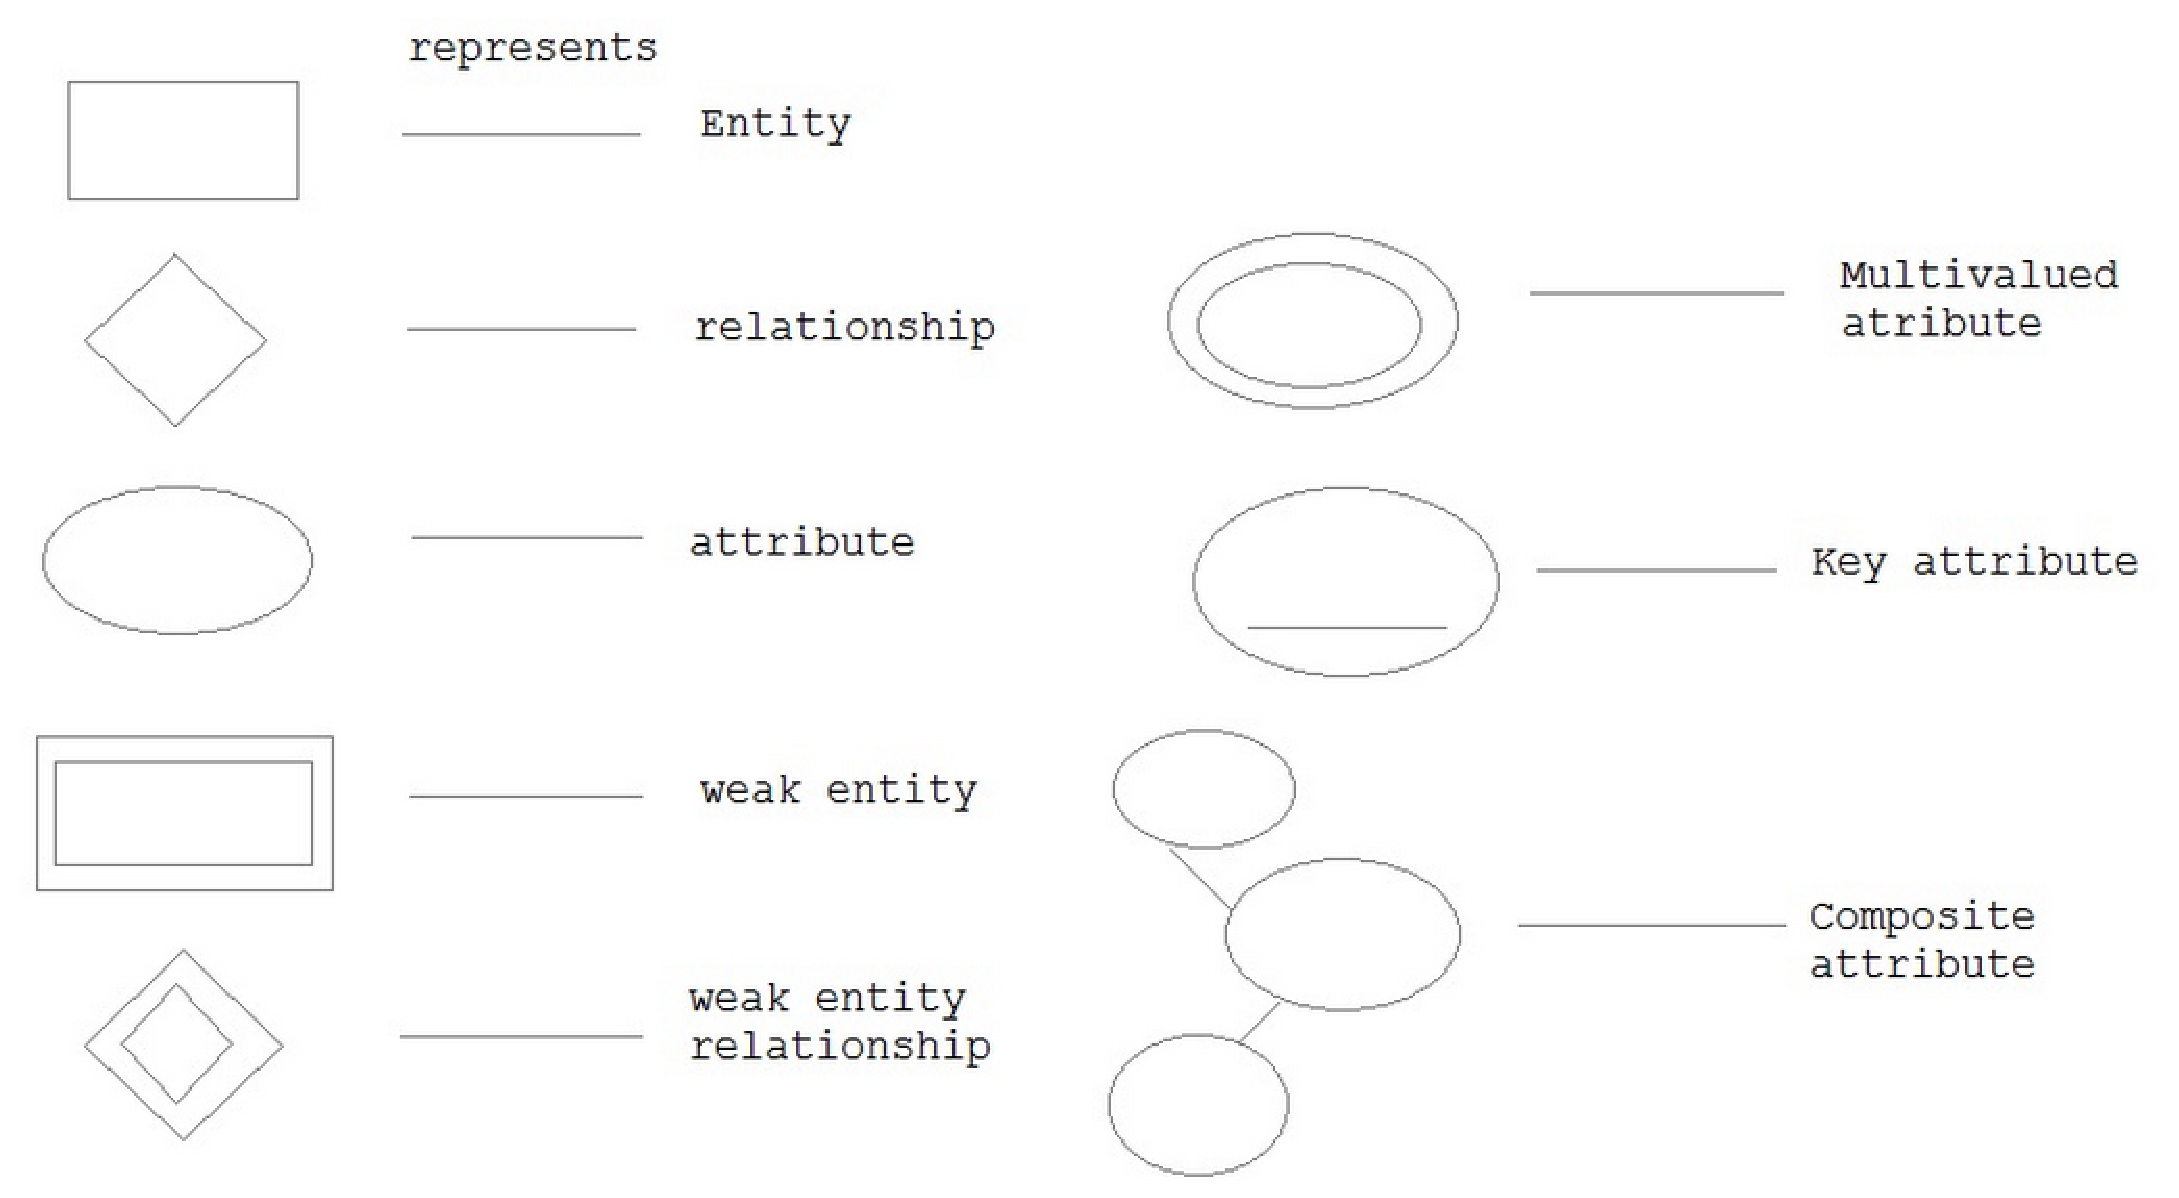
\includegraphics[height=6cm,
%     angle=0]{./images/table-relationship.eps}}
% \caption{Table relationship used in E-R diagram}
% \label{fig:table-relationship}
% \end{figure}
